\documentclass[11pt,a4paper,oneside,openany]{book}

% ---------------------------------------------------------------------------
% Lingua e codifica
% ---------------------------------------------------------------------------
\usepackage[english]{babel}
\usepackage[utf8]{inputenc}
\usepackage[T1]{fontenc}
\usepackage{lmodern}
\usepackage{microtype}

% ---------------------------------------------------------------------------
% Layout pagina "stile Word": margini 1.8 cm, interlinea 1.15,
% nessun rientro e piccolo spazio tra i paragrafi
% ---------------------------------------------------------------------------
\usepackage[a4paper,top=1.8cm,bottom=1.8cm,left=1.8cm,right=1.8cm,headheight=14pt]{geometry}
\linespread{1.15}
\usepackage[skip=4pt plus 1pt,indent=0pt]{parskip}

% Titoli compatti (niente pagina "Chapter N" enorme)
\usepackage{titlesec}
\titleformat{\chapter}[hang]{\normalfont\LARGE\bfseries}{\thechapter.}{0.5em}{}
\titlespacing*{\chapter}{0pt}{0pt}{12pt}
\titleformat{\section}{\normalfont\Large\bfseries}{\thesection}{0.5em}{}
\titlespacing*{\section}{0pt}{14pt}{6pt}
\titleformat{\subsection}{\normalfont\large\bfseries}{\thesubsection}{0.5em}{}
\titlespacing*{\subsection}{0pt}{10pt}{4pt}
\titleformat{\subsubsection}{\normalfont\normalsize\bfseries}{\thesubsubsection}{0.5em}{}
\titlespacing*{\subsubsection}{0pt}{8pt}{2pt}

% Elenchi più compatti
\usepackage{enumitem}
\setlist{topsep=2pt, itemsep=1pt, parsep=0pt, partopsep=0pt}

\newenvironment{compactitemize}{%
\begin{itemize}[topsep=0pt, partopsep=0pt, itemsep=1pt, parsep=0pt]
}{\end{itemize}}

% Spaziatura attorno a float ed equazioni ridotta
\setlength{\textfloatsep}{10pt plus 2pt minus 2pt}
\setlength{\floatsep}{8pt plus 2pt minus 2pt}
\setlength{\intextsep}{8pt plus 2pt minus 2pt}
\AtBeginDocument{%
  \setlength{\abovedisplayskip}{6pt plus 2pt minus 2pt}%
  \setlength{\belowdisplayskip}{6pt plus 2pt minus 2pt}%
  \setlength{\abovedisplayshortskip}{2pt}%
  \setlength{\belowdisplayshortskip}{4pt}%
}

% ---------------------------------------------------------------------------
% Matematica
% ---------------------------------------------------------------------------
\usepackage{amsmath}
\usepackage{amssymb}
\usepackage{mathtools}
\usepackage{latexsym}
\usepackage{gensymb}
\usepackage[makeroom]{cancel}
\DeclarePairedDelimiter\floor{\lfloor}{\rfloor}
\DeclarePairedDelimiter\ceil{\lceil}{\rceil}
\newcommand\myeq{\stackrel{\mathclap{\tiny\mbox{def}}}{=}}

% ---------------------------------------------------------------------------
% Algoritmi
% ---------------------------------------------------------------------------
\usepackage[ruled,vlined]{algorithm2e}

% ---------------------------------------------------------------------------
% Figure, tabelle, grafici
% ---------------------------------------------------------------------------
\usepackage{graphicx}
\usepackage[export]{adjustbox}
\usepackage{float}
\usepackage{placeins}
\usepackage{wrapfig}
\usepackage{caption}
\usepackage{subcaption}
\captionsetup{font=small, labelfont=bf, skip=4pt}
\usepackage{array}
\usepackage{tabularx}
\usepackage{varwidth}
\usepackage{ragged2e}
\usepackage{tikz}
\usetikzlibrary{shadows}
\usetikzlibrary{decorations.pathreplacing}
\usepackage{forest}
\usepackage{tikz-qtree}
\usepackage{pgfplots}
\pgfplotsset{compat=1.18}
\graphicspath{ {./images/} }

% ---------------------------------------------------------------------------
% Colori
% ---------------------------------------------------------------------------
\usepackage{xcolor}
\definecolor{light-gray}{gray}{0.96}
\definecolor{cyan}{RGB}{230,230,255}
\definecolor{dkgreen}{rgb}{0,0.6,0}
\definecolor{gray}{rgb}{0.5,0.5,0.5}
\definecolor{mauve}{rgb}{0.58,0,0.82}
\definecolor{iceberg}{rgb}{0.44,0.65,0.82}
\definecolor{forestGreen}{rgb}{0.13,0.55,0.13}
\newcommand{\grayScale}{0.95}
\definecolor{codeBackground}{rgb}{\grayScale,\grayScale,\grayScale}

% ---------------------------------------------------------------------------
% Link
% ---------------------------------------------------------------------------
\usepackage{url}
\usepackage{hyperref}
\hypersetup{colorlinks=true, linkcolor=black, urlcolor=blue}
\urlstyle{same}

% ---------------------------------------------------------------------------
% Codice
% ---------------------------------------------------------------------------
\usepackage{verbatim}
\usepackage{listings}
\lstset{
    language=Python,
    backgroundcolor=\color{codeBackground},
    basicstyle=\ttfamily\footnotesize,
    identifierstyle=\ttfamily,
    keywordstyle=\color{blue},
    stringstyle=\color{red},
    commentstyle=\color{forestGreen},
    numberstyle=\tiny\color{gray},
    tabsize=4,
    breaklines=true,
    breakatwhitespace=true,
    showstringspaces=false,
    showtabs=false,
    showspaces=false,
    captionpos=b,
    escapechar={|},
}

% ---------------------------------------------------------------------------
% Box
% ---------------------------------------------------------------------------
\usepackage[many]{tcolorbox}

\newtcolorbox{codicebox}[1][Python Code Example]{
    enhanced, breakable,
    colback=light-gray!80,
    colframe=black!50,
    boxrule=0.5pt, arc=2pt,
    left=4pt, right=4pt, top=4pt, bottom=4pt,
    fonttitle=\bfseries,
    title=#1,
}

\newtcolorbox{boxA}{
    breakable,
    boxrule=1.5pt,
    colframe=black,
}

\newtcolorbox{examplebox}[1][Example]{
    breakable,
    colback=cyan!5,
    colframe=cyan!60!black,
    boxrule=1pt, arc=4pt,
    left=6pt, right=6pt, top=4pt, bottom=4pt,
    fonttitle=\bfseries,
    title=#1,
}

\newtcolorbox{infobox}[1][]{
    breakable,
    colback=red!10,
    colframe=red!60!black,
    boxrule=1pt, arc=4pt,
    left=6pt, right=6pt, top=4pt, bottom=4pt,
    fonttitle=\bfseries,
    coltitle=red!10!white,
    title=#1,
}

% ---------------------------------------------------------------------------
% Intestazioni
% ---------------------------------------------------------------------------
\setcounter{tocdepth}{1}
\setcounter{secnumdepth}{3}

\usepackage{fancyhdr}
\pagestyle{fancy}
\fancyhf{}
\fancyhead[L]{\footnotesize\nouppercase{\leftmark}}
\fancyhead[R]{\footnotesize\thepage}
\renewcommand{\headrulewidth}{0.3pt}
\renewcommand{\footrulewidth}{0pt}
\renewcommand{\chaptermark}[1]{\markboth{\thechapter.\ #1}{}}
\fancypagestyle{plain}{%
    \fancyhf{}
    \fancyhead[R]{\footnotesize\thepage}
    \renewcommand{\headrulewidth}{0pt}
}

% ===========================================================================
\begin{document}
\begin{titlepage}
  \newgeometry{top=2cm, bottom=2cm, left=2cm, right=2cm}
  \begin{center}
  
      {\Large \textbf{Università degli Studi di Modena e Reggio Emilia}} \\[2mm]
      {\large Dipartimento di Ingegneria "Enzo Ferrari"} \\[15mm]
  
      \vspace{\stretch{0.3}}
  
      
      {\large Master Computer Science Degree} \\
      
        \vspace{0.5cm}
      
      {\huge \textbf{Machine Learning and Deep Learning}} \\

  
      \vspace{\stretch{1}}
  
      \begin{flushleft}
          \textbf{Professore:} Simone Calderara e Angelo Porrello \\[5mm]
          % \textbf{Correlatore:} Nome Cognome % <-- opzionale
      \end{flushleft}
  
      \vspace{1.2cm}
  
      \begin{flushright}
          \textbf{Studente:} Rocco Lubino \\
      \end{flushright}
  
      \vspace{2cm}
      {\large Anno Accademico 2025/2026}
  
  \end{center}
\end{titlepage}

\restoregeometry

\tableofcontents
\clearpage

\chapter{Logistic Regression and Optimizer}
Making a step back to the basics, we are given a training set $\{(X_i, Y_i)\}_{i=1}^N$, with $X_i \in \mathbb{R}^m$ and $Y_i \in \{0,1\}$ for all $i = 1, \dots, N$. Where:
\begin{compactitemize}
    \item $N$ is the number of training examples;
    \item each $X_i$ is a vector of $m$ features, i.e. $X_i = [x_{i1}, x_{i2}, \dots, x_{im}]$;
    \item each $Y_i$ is a binary label, i.e. $Y_i \in \{0,1\}$.
\end{compactitemize}

\section{Logistic Regression}
Logistic Regression is a \emph{probabilistic discriminative classifier}, which means that it models the posterior probability $P(Y|X)$ directly, without modeling the prior distribution $P(X)$ or the likelihood $P(X|Y)$. 
In the binary case, the posterior probability is models as:
\begin{equation}
    P(Y=1|X) = \frac{1}{1 + e^{w^Tx + b)}}
\end{equation}
\begin{equation}
    P(Y=0|X) = 1 - P(Y=1|X) = \frac{e^{(w^Tx + b)}}{1 + e^{(w^Tx + b)}}
\end{equation}
By computing the decion boundary, we can see that the model is \emph{linear}:
\begin{equation}
    log P(Y=0|x)-log P(Y=1|x) = w^T x + b 
\end{equation}
The classification function is:
\begin{equation}
    f_{LR}(x)=argmax_{c \in \mathbb{Y}} P(Y=c|x) 
\end{equation}

If we want, we can extend the model to the multi-class case with K classes, in the following way:
\begin{equation}
    P(Y=c|x)=\frac{e^{w_c^T x + b_c}}{\sum_{l=1}^{K-1} e^{w_l^T x + b_l}}
\end{equation}
\begin{equation}
    P(Y=K|x)=\frac{1}{\sum_{l=1}^{K-1} e^{w_l^T x + b_l}}
\end{equation}
Also in the mutli-class case, the classification function is the same.

\subsection{Learning Logistic Regression}
The logistic regression parameters $\theta=(w_c,b_c), c \in \mathbb{Y}$ are selected to optimize the conditional log likelihood of the tables given a dataset $\mathbb{D}=\{(x_i,y_i), i= 1:n\}$:
\begin{equation}
    \theta_*= argmax_{\theta}\mathbb{L}(\theta,D) = argmax_{\theta} \sum_{i=1}^{n} log P(Y=y_i|X=x_i)
\end{equation}
However, the function $\mathbb{L}(\theta,D)$ can not be maximized analytically. Learning the parameters is done by numerical optimization methods, such as Gradient Descent or Newton's Method.

\subsection{Example of binary Logistic Regression}
Let's consider a simple example of binary logistic regression, given 2 classes $y \in 0,1$ and dataset $\mathbb{D}$ by absorbing the bias term in the weights:
\begin{equation}
    P(Y=1|x) = \frac{e^{w^Tx}}{1 + e^{w^Tx}}
\end{equation}
\begin{equation}
    P(Y=0|x) =  \frac{1}{1 + e^{w^Tx}}
\end{equation}

The conditional log likelihood over the dataset beacomes:
\begin{equation}
    \begin{aligned}
    &\mathcal{L}(\theta\mid D)
    =\sum_{i=1}^{N} \Big[ y_i\log P(Y=1\mid x_i) + (1-y_i)\log P(Y=0\mid x_i)\Big] \\[6pt]
    &\quad= \sum_{i=1}^{N} \Bigg[ y_i\log\!\left(\frac{e^{w^{T}x_i}}{1+e^{w^{T}x_i}}\right)
    +(1-y_i)\log\!\left(\frac{1}{1+e^{w^{T}x_i}}\right) \Bigg] \\[6pt]
    &\quad= \sum_{i=1}^{N} \Bigg[ y_i\big( w^{T}x_i - \log(1+e^{w^{T}x_i})\big)
    + (1-y_i)\big( -\log(1+e^{w^{T}x_i})\big) \Bigg] \\[6pt]
    &\quad= \sum_{i=1}^{N} \Big[ y_i w^{T}x_i - y_i\log(1+e^{w^{T}x_i}) - (1-y_i)\log(1+e^{w^{T}x_i})\Big] \\[6pt]
    &\quad= \sum_{i=1}^{N} \Big[ y_i w^{T}x_i - \log(1+e^{w^{T}x_i})\big(y_i + (1-y_i)\big)\Big] \\[6pt]
    &\quad= \sum_{i=1}^{N} \Big[ y_i w^{T}x_i - \log(1+e^{w^{T}x_i})\Big].
    \end{aligned}
\end{equation}
If you are a good observer, you will notice that the last equation is the same as the one of the \emph{cross-entropy loss} for a binary classification problem. This is not a coincidence, in fact maximizing the conditional log likelihood is equivalent to minimizing the cross-entropy loss.
    
\textbf{Notes:} We need to learn the parameters $w$ of a parametric function that maps X to Y such that some error is as low as possible on the training set.

\subsection{Logistic Regression classification rule}
The function for classification has the following form:
\begin{equation}
    \mathbb{F}(X_i, w) = \sigma(w^{T}X_i), 
    \quad \text{where} \quad 
    \sigma(x) = \frac{1}{1+e^{-x}} = \frac{e^{x}}{1+e^{x}}.
\end{equation}
The principal thing to know are:
\begin{compactitemize}
    \item $\sigma$ is the \emph{sigmoid function}:the vantage of using the sigmoid, despite a step function, is that it is differentiable and map smoothly the input space to the (0,1) interval that can be interpreted as a probability;
    \item $w$ is a vector in $\mathbb{R}^m$, and is called the \emph{weight vector};
    \item $w$ is inizialized randomly, but will improve ad training goes on;
\end{compactitemize}

\begin{figure}[H]
    \centering
    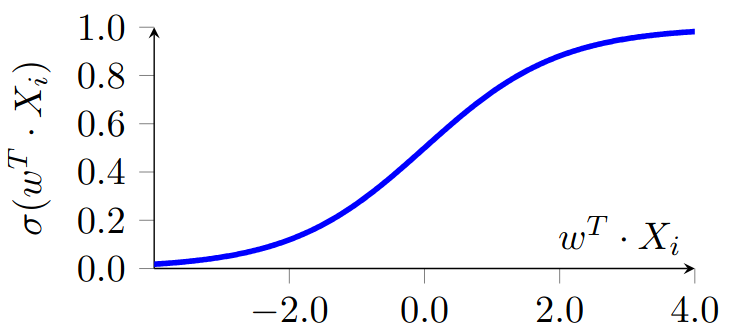
\includegraphics[width=0.4\textwidth]{images/sigmoid.png}
    \caption{Sigmoid function}
    \label{fig:sigmoid_function}
\end{figure}

During training, we want to find the best $w$ that minimize the error on the training set. The error is computed with the \emph{cross-entropy loss function}:
\begin{equation}
    \mathcal{L}(w) = -\frac{1}{N}\sum_{i=1}^{N} \Big[ Y_i \log(\mathbb{F}(X_i,w)) + (1-Y_i)\log(1-\mathbb{F}(X_i,w)) \Big]
\end{equation}

\subsection{Gradient Descent}
To minimize the loss function, we can use the \emph{Gradient Descent} algorithm. The idea is to compute the gradient of the loss function with respect to the weights, and then update the weights in the opposite direction of the gradient. If we considere a function $f(\theta)$, the gradient descent update can be expresses  as:
\begin{equation}
    \theta_j := \theta_j - \alpha \, \frac{\partial}{\partial \theta_j} f(\theta) \text{ ,for all parameter} \theta_j
\end{equation}
Where:
\begin{compactitemize}
    \item $\theta_j$ is the $j$-th parameter of the model;
    \item $\alpha$ is the \emph{learning rate}, a small positive value that controls the step size of the update;
    \item $\frac{\partial}{\partial \theta_j} f(\theta)$ is the partial derivative of the function with respect to the $j$-th parameter.
\end{compactitemize}


\begin{figure}[H]
    \centering
    \begin{minipage}{0.45\textwidth}
        \centering
        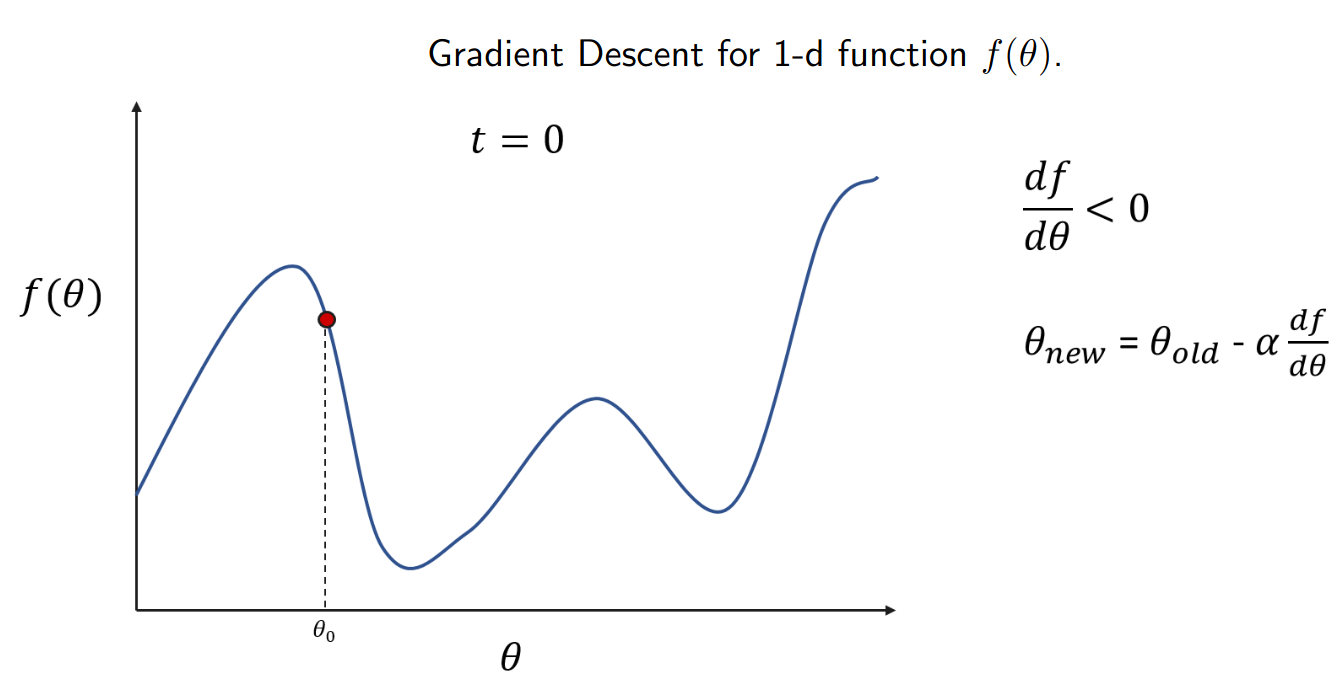
\includegraphics[width=\textwidth]{images/GD_start.png}
        \caption{Gradient Descent Start}
        \label{fig:Gradient_Descent_Start}
    \end{minipage}
    \hfill
    \begin{minipage}{0.45\textwidth}
        \centering
        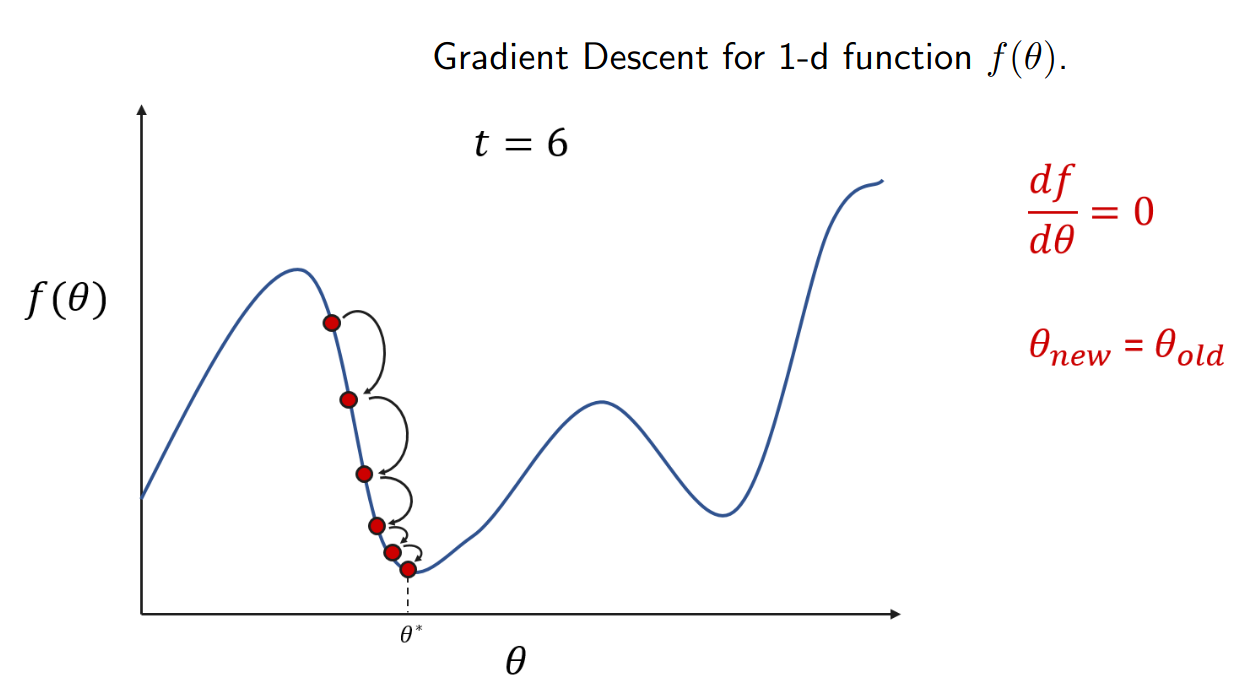
\includegraphics[width=\textwidth]{images/GD_end.png}
        \caption{Gradient Descent End}
        \label{fig:Gradient_Descent_End}
    \end{minipage}
    \label{fig:Gradient_Descent}
\end{figure}

Choosing the right learning rate $\alpha$ is essential to correctly proceed towards the minimum. Astep too small could lead to an extremely slow convergence. If the step is too big, theoptimizer could overshoot the minimum or even diverge.

\begin{figure}[H]
    \centering
    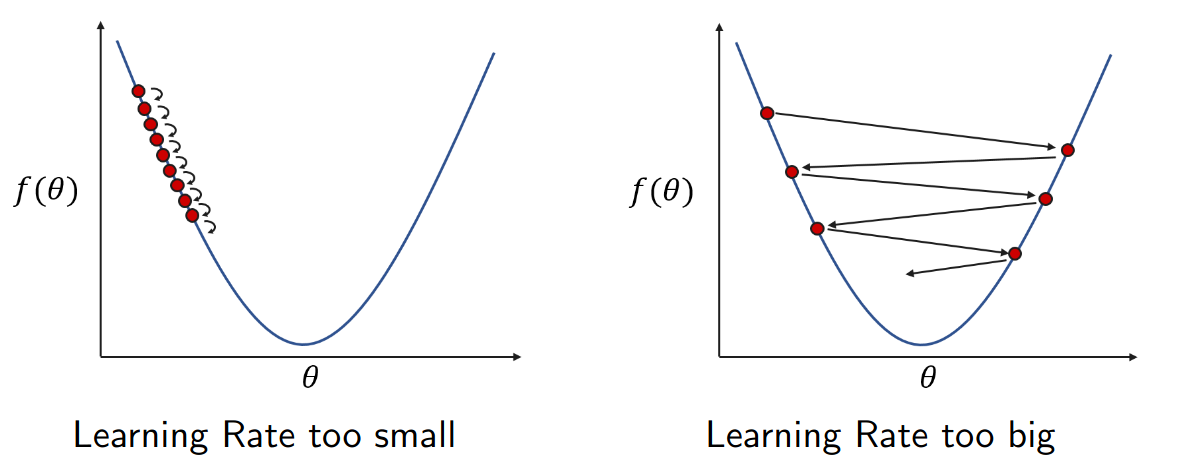
\includegraphics[width=0.8\textwidth]{images/LR.png}
    \caption{Learning Rate effect}
    \label{fig:Learning_Rate_effect}
\end{figure}

Turns out that if the function is convex, gradient descent will converge to the global minimum. For non-convex functions, it may converge to local minima.

\begin{figure}[H]
    \centering
    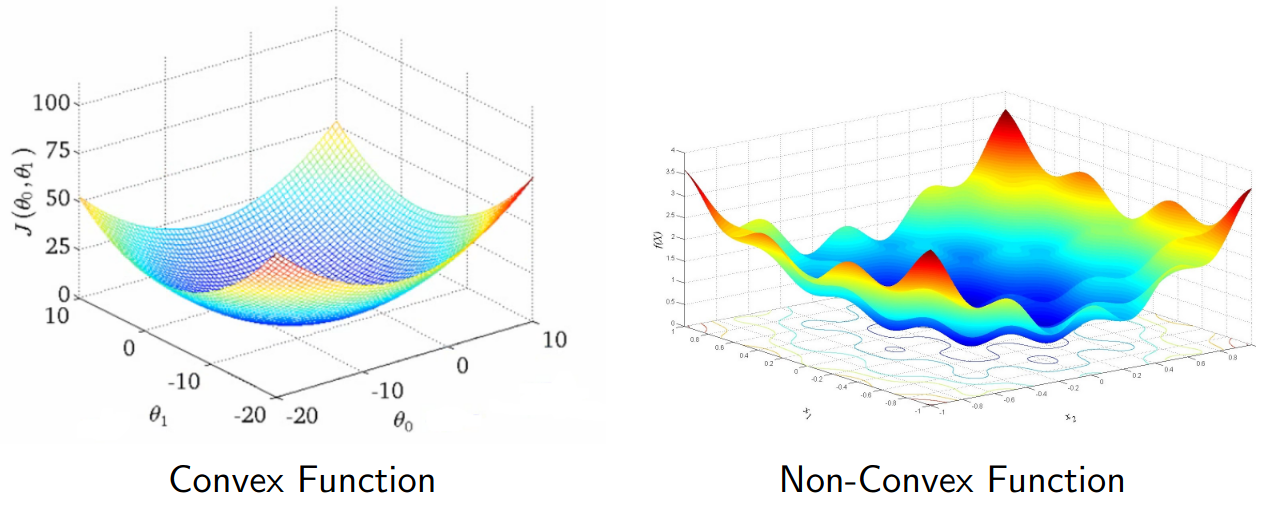
\includegraphics[width=0.8\textwidth]{images/convex_or_no.png}
    \caption{Convex or not Convex function}
    \label{fig:Convex_or_not_Convex_function}
\end{figure}

\textbf{Notes:} If we stop in a local minimum, we are not figure out with the basic GD. There are some techniques that can try to avoid or escape from local minima, like adding noise to the gradient or using momentum.

\subsection{Mathematical explanation of the weight update}
Back to our logistic regression, we want to compute the gradient of the loss function with respect to the weights. In the first we simplify the loss function:
\begin{equation}
    \begin{aligned}
    L(w) &= -\frac{1}{N} \sum_{i=1}^{N} \Big[ Y_i \log(F(X_i, w)) + (1 - Y_i) \log(1 - F(X_i, w)) \Big] \\
         &= -\frac{1}{N} \sum_{i=1}^{N} \Bigg[ 
                Y_i \log \left( \frac{e^{w^T X_i}}{1 + e^{w^T X_i}} \right) 
              + (1 - Y_i) \log \left( \frac{1}{1 + e^{w^T X_i}} \right) 
            \Bigg] \\
         &= -\frac{1}{N} \sum_{i=1}^{N} \Big[ 
                Y_i (w^T X_i) - Y_i \log(1 + e^{w^T X_i}) 
              + (Y_i - 1) \log(1 + e^{w^T X_i}) 
            \Big] \\
         &= -\frac{1}{N} \sum_{i=1}^{N} \Big[ 
                Y_i (w^T X_i) - \log(1 + e^{w^T X_i}) 
            \Big]
    \end{aligned}
\end{equation}
Now we compute the partial derivative with respect to $w_j$:
\begin{equation}
    \begin{aligned}
    \frac{\partial L(w)}{\partial w_j} 
    &= -\frac{1}{N} \sum_{i=1}^{N} \Big[ Y_i x_i^{(j)} - \frac{e^{w^T X_i}}{1 + e^{w^T X_i}} x_i^{(j)} \Big] \\
    &= -\frac{1}{N} \sum_{i=1}^{N} \Big[ \big( Y_i - \frac{e^{w^T X_i}}{1 + e^{w^T X_i}} \big) x_i^{(j)} \Big] \\
    &= -\frac{1}{N} \sum_{i=1}^{N} \Big[ \big( Y_i - F(X_i, w) \big) x_i^{(j)} \Big]
    \end{aligned}
\end{equation}
Now we can form the gradient vector and update the weights:
\begin{equation}
    \frac{\partial L(w)}{\partial w} =
    \begin{bmatrix}
    \frac{\partial L(w)}{\partial w_1} \\
    \frac{\partial L(w)}{\partial w_2} \\
    \vdots \\
    \frac{\partial L(w)}{\partial w_m}
    \end{bmatrix}
    =
    -\frac{1}{N}
    \begin{bmatrix}
    \sum_{i=1}^{N} \big(Y_i - F(X_i, w)\big) x_i^{(1)} \\
    \sum_{i=1}^{N} \big(Y_i - F(X_i, w)\big) x_i^{(2)} \\
    \vdots \\
    \sum_{i=1}^{N} \big(Y_i - F(X_i, w)\big) x_i^{(m)}
    \end{bmatrix}
    =
    -\frac{X^T \cdot (Y - F(X, w))}{N}
    \end{equation}

\textbf{Note:} Each row of the matrix is a number.

In the end we update weights with the following rule:
\begin{equation}
    w \gets w - \alpha \frac{\partial L(w)}{\partial w}
\end{equation}


\section{Optimizers}
Gradient descent is often used in machine learning to minimize a cost function, usually also called objective or loss function and denoted $L()$ or $J()$.
The cost function depends on the model’s parameters and serves as a proxy for evaluating the
model's performance. Generally speaking, in this framework minimizing the cost equals to
maximizing the effectiveness of the model.

\subsection{Stochastic Gradient Descent (SGD)}
In principle, to perform a single update step, you should run through all your training examples. This is known as \textbf{batch gradient descent}.
A different strategy is \textbf{minibatch stochastic gradient descent}. In this case, only a small subset of the training dataset is considered at each update step.
In the extreme case in which only a random example of the training set is considered to perform the update step, we talk of \textbf{stochastic gradient descent}.
This methods is typycally called vanilla SGD, and not often used in practice. 

\subsection{Advanced Optimizer}
The advanced optmizer are typycally characterized by the presence of two elements:
\begin{compactitemize}
    \item \textbf{Momentum}: using an exponentially weighted moving average of past gradients to smooth out the trajectory of the optimization, allowing faster convergence and reducing oscillations.
    \item \textbf{Adaptive Learning Rate}: scaling each parameter's learning rate by running average of the magnitude of the past gradients.
\end{compactitemize}

\begin{figure}[H]
    \centering
    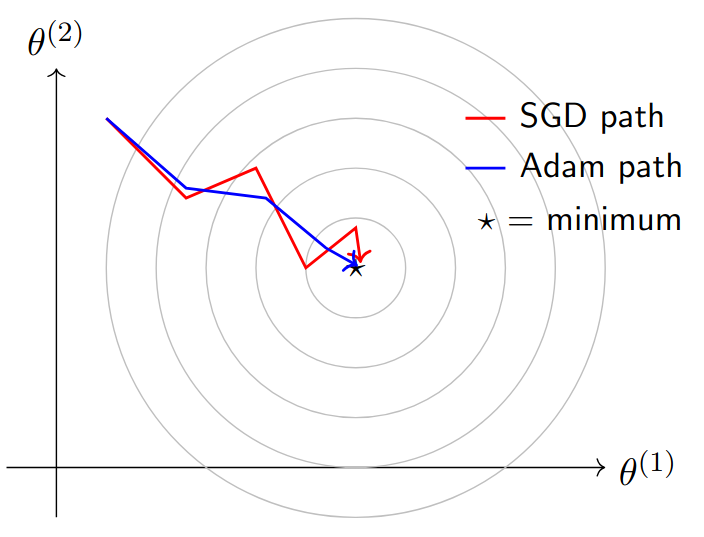
\includegraphics[width=0.5\textwidth]{images/ADAM.png}
    \caption{Advanced Optimizer}
    \label{fig:Advanced_Optimizer}
\end{figure}

\subsection{ADAM}
ADAM (short for Adaptive Moment Estimation) is an optimization algorithm that combines the benefits of both Momentum and RMSProp. It computes adaptive learning rates for each parameter by maintaining running averages of both the gradients and their squares.
The ADAM algorithm can be summarized as follows:
\begin{align}
    g_t &= \frac{\partial L}{\partial \theta_t} && \text{Gradient at step } t \\
    m_t &= \beta_1 m_{t-1} + (1 - \beta_1) g_t && \text{First moment (mean) estimate} \\
    v_t &= \beta_2 v_{t-1} + (1 - \beta_2) g_t^2 && \text{Second moment (variance) estimate} \\
    \hat{m}_t &= \frac{m_t}{1 - \beta_1^t} && \text{Bias-corrected first moment} \\
    \hat{v}_t &= \frac{v_t}{1 - \beta_2^t} && \text{Bias-corrected second moment} \\
    \theta_{t+1} &= \theta_t - \alpha \frac{\hat{m}_t}{\sqrt{\hat{v}_t} + \epsilon} && \text{Weight update}
\end{align}
\textbf{Bias correction} prevents the moment estimates from being biased toward zero, as both are initialized at zero, helping early-stage stability.\\
Typical default values for the hyperparameters are:
\begin{compactitemize}
    \item $\beta_1 = 0.9$: controls the decay rate of the moving average of the first moment (mean).
    \item $\beta_2 = 0.999$: controls the decay rate of the moving average of the second moment (variance).
    \item $\epsilon = 10^{-8}$: a small constant added to the denominator to prevent division by zero.
    \item $\alpha$: learning rate, typically set to $0.001$.
\end{compactitemize}

Let's summarize the main advantages and disadvantages of ADAM:\\
ADAM advanrages:
\begin{compactitemize}
    \item Works well out-of-the-box with minimal tuning.
    \item Handles noisy and sparse gradients effectively.
    \item Fast convergence in many pratical problems.
\end{compactitemize}
ADAM disadvantages:
\begin{compactitemize}
    \item May sometimes lead to worse generalization than SGD with momentum.
    \item Extra memory cost for moment estimates $(m_t,v_t)$.
\end{compactitemize}

    

\chapter{Multi Layer Perceptron (MLP)}

\section{Difference between Machine Learning and Deep Learning}
The performance of machine learning algorithms heavily depends on the way we represent the data. These discrete pieces of information that we use as a proxy to model the complexity of the world are usually called features. Generally speaking, for a long time, these features have been handcrafted differently for each task at hand. However, traditional machine learning methods are inherently limited by this feature extraction process, since the quality of the final model strongly relies on the quality of the manually designed features.

In contrast, deep learning algorithms remove this limitation by simultaneously performing both feature extraction and learning the function that classifies (or predicts) the data within the same model. This means that the network itself learns the most suitable representations directly from raw data, without requiring handcrafted features. Moreover, in a deep neural network, it is not straightforward to pinpoint where feature extraction ends and classification begins, as both processes are deeply intertwined within the layered structure of the model.

\begin{figure}[H]
    \centering
    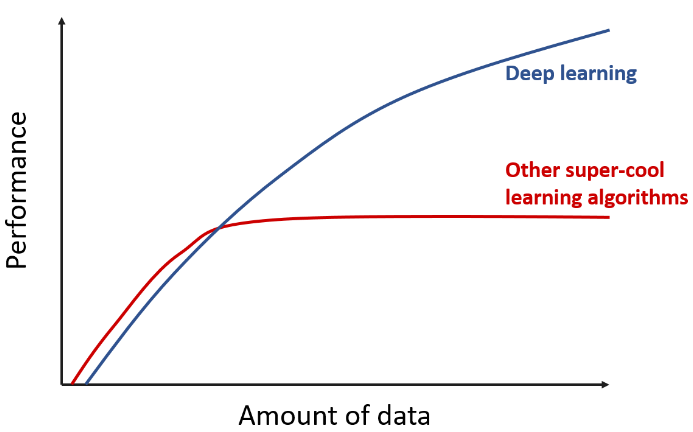
\includegraphics[width=0.5\textwidth]{images/size_matter.png}
    \caption{Why size matter}
    \label{fig:size_matter}
\end{figure}

\section{One step back: Linear classifier}
For the purpose of this lecture, we will stick to the task of image classification. 
Let’s assume we have a training dataset of $N$ images

\begin{equation}
x_i \in \mathbb{R}^D, \quad i = 1, \ldots, N
\end{equation}

that we want to classify into $K$ distinct classes. 
Thus, the training set is made of pairs

\begin{equation}
(x_i, y_i), \quad y_i \in \{1, \ldots, K\}
\end{equation}

Our goal is to define a function

\begin{equation}
f : \mathbb{R}^D \rightarrow \mathbb{R}^K
\end{equation}

that maps images to class scores.

As a real-world example, let’s take the CIFAR-10 dataset, which consists of 
$N = 60{,}000$ $32 \times 32$ RGB images belonging to 10 different classes. 

\begin{figure}[H]
    \centering
    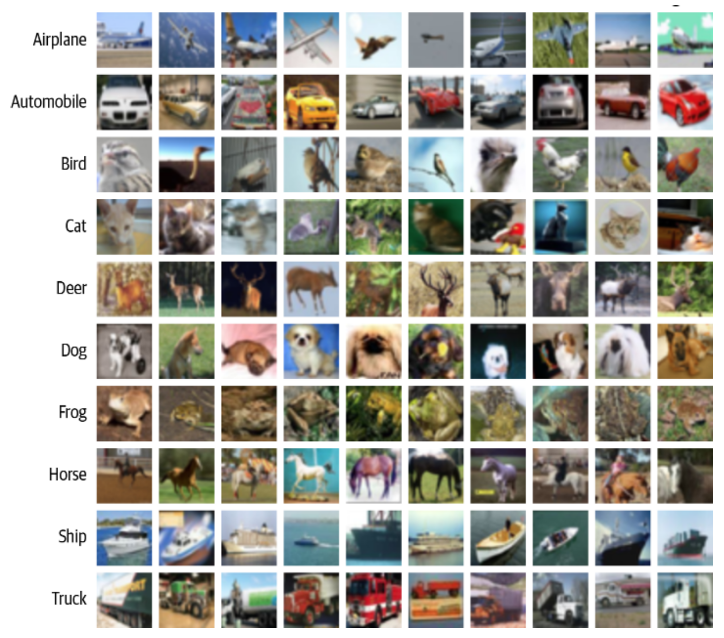
\includegraphics[width=0.5\textwidth]{images/cifrar_10.png}
    \caption{Why Cifrar-10 dataset}
    \label{fig:cifrar_10}
\end{figure}

Each image has dimensions $32 \times 32 \times 3$, and can therefore be represented as a column vector

\begin{equation}
x_i \in \mathbb{R}^{3072}
\end{equation}

We can now define a linear mapping:

\begin{equation}
f(x_i, W, b) = W x_i + b
\end{equation}

where the parameters are:

\begin{equation}
W \in \mathbb{R}^{10 \times 3072}, \quad b \in \mathbb{R}^{10}
\end{equation}

The role of the weight matrix is to learn how each pixel contributes to the class scores. 
The bias term, instead, is crucial because it allows us to \textbf{translate the decision boundaries} of the classes 
with respect to the same reference system. 
Without the bias, all class boundaries would be constrained to pass through the origin, 
which would unnecessarily limit the flexibility of the classifier.

Intuitively, our goal is to learn the parameters from the training data, when a new test image $x_i^{\text{test}}$ is presented to the model, the score of the correct class is higher that the scores of other classes-

\begin{figure}[H]
    \centering
    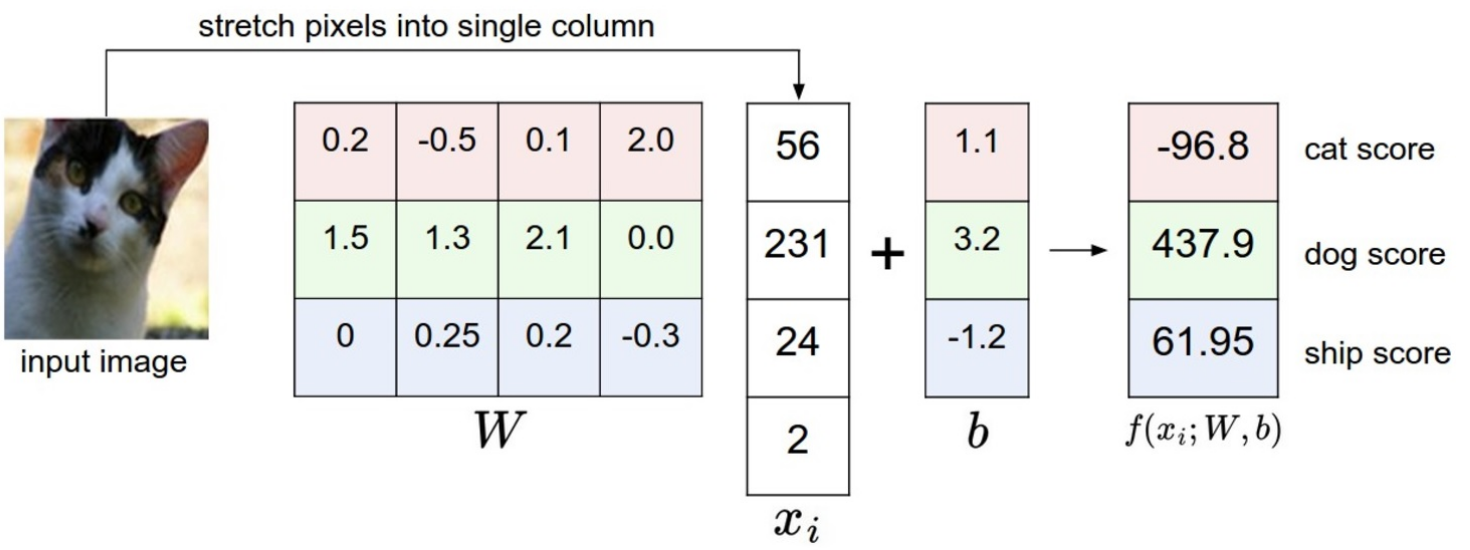
\includegraphics[width=0.8\textwidth]{images/linear_ex.png}
    \caption{Example of mapping an image to a score. For the sake of the visualization, here the image is assumed to have only 4 grayscale pixels.}
    \label{fig:linear_ex}
\end{figure}

\subsection{Logistic Regression}

If we add a sigmoid non-linearity to our linear mapping, we get a logistic regression classifier:

\begin{equation}
f(x_i, W, b) = \sigma(W x_i + b), \quad \text{where } \sigma(x) = \frac{1}{1 + e^{-x}}
\end{equation}

This model can be trained by optimizing the so-called \textit{binary cross-entropy loss}:

\begin{equation}
L(W, b) = - \frac{1}{m} \sum_{i=1}^{m} \Big( y_i \log(f_{x_i}) + (1 - y_i) \log(1 - f_{x_i}) \Big)
\end{equation}

Here, $m$ is the number of examples in the training set, and $f_{x_i}$ (with an abuse of notation) denotes $f(x_i, W, b)$.  

Let’s try to understand better the binary cross-entropy loss:

\begin{equation}
L(W, b) = - \frac{1}{m} \sum_{i=1}^{m} \Big( y_i \log(f_{x_i}) + (1 - y_i) \log(1 - f_{x_i}) \Big)
\end{equation}

Note that $y_i \in \{0, 1\}$, since this is a binary classification task.  

\begin{figure}[H]
    \centering
    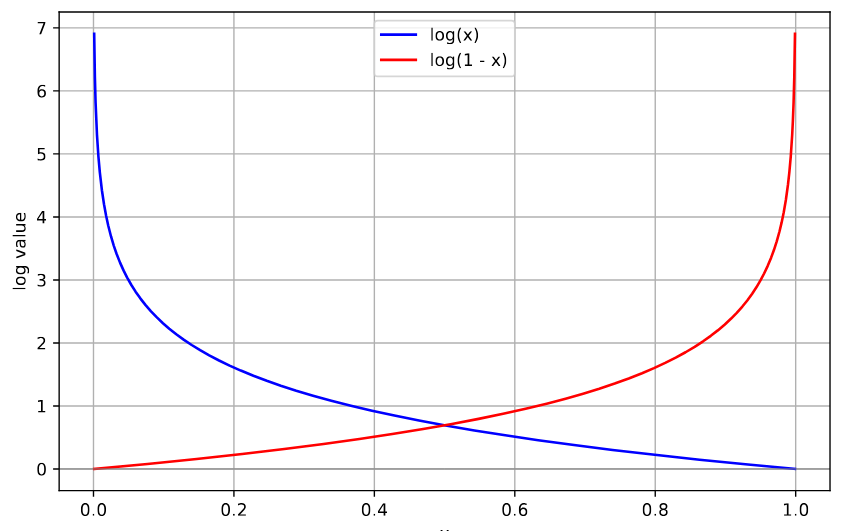
\includegraphics[width=0.5\textwidth]{images/log.png}
    \caption{log(x) and log(1-x) functions}
    \label{fig:log}
\end{figure}

The label $y_i$ act as a selector. For positive examples we penalize predictions close to zero. For negative examples we penalize predictions close to one.

\subsection{Softmax Classifier}
Softmax Classifier generalizes Logistic Regression to multi-class problems. We first define the softmax function:
\begin{equation}
\text{softmax}_j(z) = \frac{e^{z_j}}{\sum_{K} e^{z_j}}
\end{equation}

It takes a vector of arbitary real-valued scores and squashes it to a vector of values between zero and one that sum to one. Example:

\[
z =
\begin{bmatrix}
1.2 \\
5.1 \\
2.7
\end{bmatrix}, 
\quad
\text{softmax}(z) =
\begin{bmatrix}
0.018 \\
0.90 \\
0.08
\end{bmatrix}
\]

\textbf{Note:} ThSoftmax transforms the scores into probabilities that sum to 1, but the relative ratios of the original scores are distorted because of the exponential, which emphasizes larger values and suppresses smaller ones.

In the softmax classifier, the scores of the linear function mapping 

\begin{equation}
f(x_i, W) = W x_i
\end{equation}

are interpreted as unnormalized log probabilities. To train the classifier we optimize the cross-entropy loss:

\begin{equation}
L = \sum_i y^{\text{true}}_i \log(y^{\text{pred}}_i)
\end{equation}

where $y^{\text{true}}_i$ is the ground truth output distribution and $y^{\text{pred}}_i$ is the predicted output distribution. 

In practice, $y^{\text{true}}_i$ is a one-hot vector selecting the output of the correct label. 

\textbf{Notice:} the softmax classifier has the appealing property to produce an easy-to-interpret output, 
that is, the normalized score confidence for each class.

\section{Modelling a Neuron}

Neural Networks are a mathematical model \textbf{coarsely} inspired by the way our own brain works

\begin{figure}[H]
    \centering
    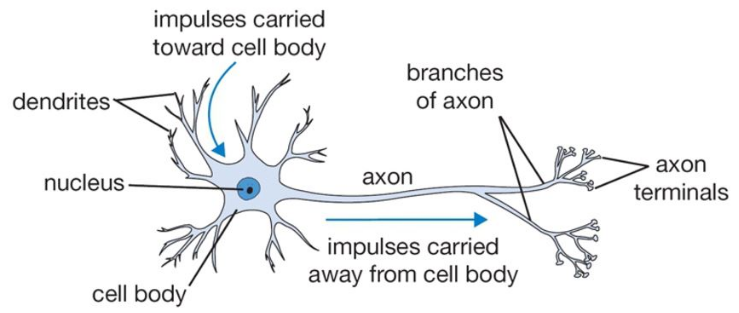
\includegraphics[width=0.6\textwidth]{images/neuron.png}
    \caption{Neuron model}
    \label{fig:neuron}
\end{figure}

Neurons are the basic computational unit of our brain. Approximately 86 billion neurons can
be found in the human nervous system and they are connected with approximately $10^14$-$10^15$
\textbf{synapses}. Each neuron receives input signals from its \textbf{dendrites} and produces output signals
along its (single) \textbf{axon}. The axon eventually branches out and connects via synapses to
dendrites of other neurons.

More formally, we can model a single \textbf{neuron} as follows:

\begin{figure}[H]
    \centering
    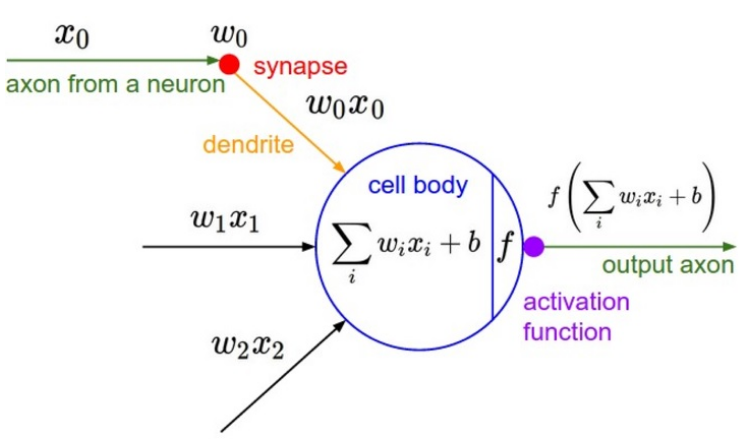
\includegraphics[width=0.5\textwidth]{images/artificial_neuron.png}
    \caption{Artificial Neuron model}
    \label{fig:artificial_neuron}
\end{figure}

Each neuron can have multiple inputs. The neuron's output is the dot product between the inputs and its weughts, plus the bias; then an activation function is applied, generally a non-linearity.

It's easy to see that a single neuron can be used to implement a binary classifier. Indeed, when loss is applied to the output of the neuron, we can optimize a \textbf{binary Softmax classifier} (a.k.a. Logistic Regression).


\subsection{Neuron Activation Functions}

Activation functions are non-linear functions computed on the output of each neuron. 
Commonly used activations include \textbf{sigmoid}, \textbf{tanh}, and \textbf{ReLU}, 
although more complex activations also exist.

\subsubsection{Sigmoid}
The sigmoid activation function is defined as:
\begin{equation}
\sigma(x) = \frac{1}{1 + e^{-x}}
\end{equation}

\begin{compactitemize}
  \item Squashes any real-valued input into the range $[0, 1]$.
  \item Historically widely used, but now less common.
  \item \textbf{Drawbacks:}
  \begin{compactitemize}
    \item Saturates for large positive or negative values, leading to vanishing gradients.
    \item Output is not zero-centered, which can slow down convergence.
  \end{compactitemize}
\end{compactitemize}

\begin{figure}[H]
    \centering
    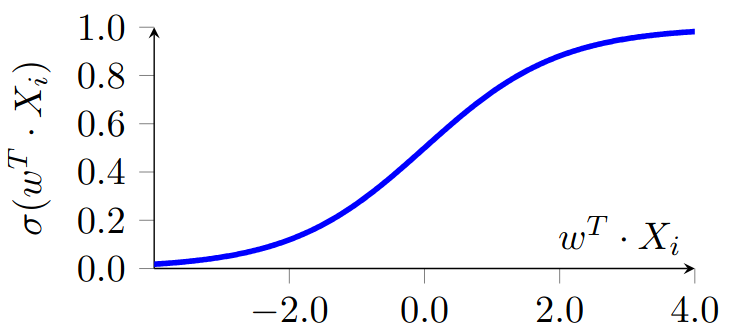
\includegraphics[width=0.5\textwidth]{images/sigmoid.png}
    \caption{Sigmoid activation function}
    \label{fig:sigmoid}
\end{figure}

\subsubsection{Tanh}
The tanh activation function is a scaled sigmoid:
\begin{equation}
\tanh(x) = 2\sigma(x) - 1
\end{equation}

\begin{compactitemize}
  \item Squashes input to the range $[-1, 1]$.
  \item Output is zero-centered.
  \item \textbf{Drawback:} activation can still saturate for large inputs, causing vanishing gradients.
\end{compactitemize}


\begin{figure}[H]
    \centering
    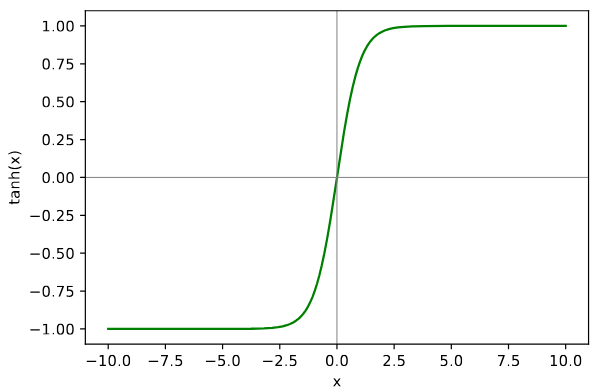
\includegraphics[width=0.5\textwidth]{images/tanh.png}
    \caption{Tanh activation function}
    \label{fig:tanh}
\end{figure}

\subsubsection{ReLU (Rectified Linear Unit)}
The ReLU activation function is defined as:
\begin{equation}
\text{ReLU}(x) = \max(0, x)
\end{equation}

\begin{compactitemize}
  \item Accelerates convergence of SGD compared to sigmoid/tanh.
  \item Simple to implement: threshold at 0, no expensive exponential computations.
  \item \textbf{Solves positive saturation:}
  \begin{compactitemize}
    \item For $x>0$, gradient is 1 → no vanishing gradient for positive values.
    \item For $x\le0$, gradient is 0 → negative part is inactive.
  \end{compactitemize}
\end{compactitemize}


\begin{figure}[H]
    \centering
    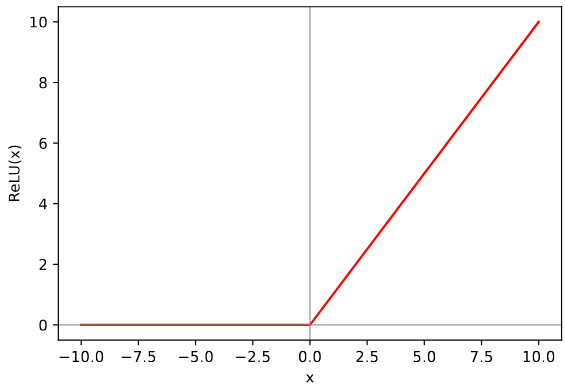
\includegraphics[width=0.5\textwidth]{images/relu.png}
    \caption{ReLU activation function}
    \label{fig:relu}
\end{figure}

\subsubsection{Why Non-linear Activations?}
\begin{compactitemize}
  \item Composition of linear functions is still linear.
  \item Without nonlinearities, a neural network reduces to a single linear transformation:
  \begin{equation}
  f(x) = \phi(W_2 \phi(W_1 x)) \quad \text{with nonlinear activation } \phi
  \end{equation}
  \item Removing the nonlinearities:
  \begin{equation}
  f(x) = W_2 W_1 x = W x
  \end{equation}
  \item Clearly still linear, so no hierarchical feature learning would occur.
\end{compactitemize}

\section{Neural Networks}
When we connect an ensemble of neurons in a graph is when the magic happens and we get an actual Multilayer Perceptron (MLP)
Neural Networks are arranged in layers, with one input layer, one output layer, and N hidden layers in the middle.

\begin{figure}[H]
    \centering
    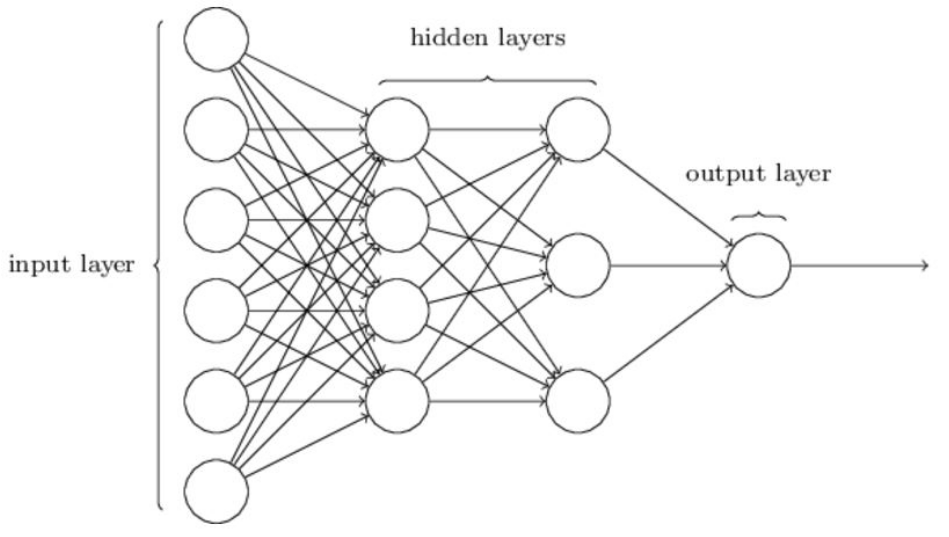
\includegraphics[width=0.4\textwidth]{images/NN.png}
    \caption{A simple Neural Network with 2 hidden layers}
    \label{fig:NN}
\end{figure}

The 4-layer network previously depicted can be expressed as:

\begin{equation}
\text{out} = \phi \Big( W_3 \, \phi \big( W_2 \, \phi ( W_1 x ) \big) \Big)
\end{equation}

where:

\begin{compactitemize}
  \item $\phi$ is the activation function.
  \item $x \in \mathbb{R}^6$ is the input.
  \item $W_1 \in \mathbb{R}^{4 \times 6}$ are the weights of the first layer.
  \item $W_2 \in \mathbb{R}^{4 \times 3}$ are the weights of the second layer.
  \item $W_3 \in \mathbb{R}^{1 \times 3}$ are the weights of the third layer.
\end{compactitemize}

\noindent
\textbf{Note:} To ease notation, biases have been incorporated into the weight matrices $W$.

\subsection{Forward propagation}
Forward propagation is the process of computing the output of the neural network given an input.
It involves passing the input through each layer of the network, applying the weights, biases, and activation functions at each step.

\begin{figure}[H]
    \centering
    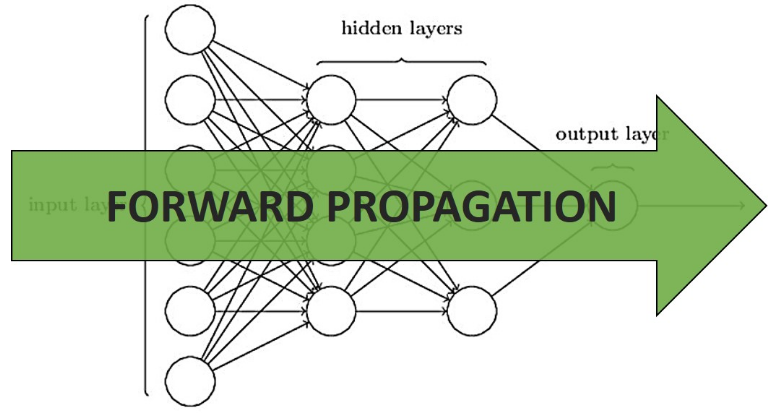
\includegraphics[width=0.4\textwidth]{images/forward.png}
    \caption{Forward propagation in a Neural Network}
    \label{fig:forward}
\end{figure}

\subsection{Representational Power}

It has been shown that any continuous function $f(x)$ can be approximated at arbitrary precision $\epsilon > 0$ by a neural network $g(x)$ with at least one hidden layer:

\begin{equation}
\forall x, \quad |f(x) - g(x)| < \epsilon
\end{equation}

\begin{compactitemize}
  \item Neural networks with at least one hidden layer are referred to as \textbf{universal approximators}.
  \item In practice, networks with more layers often outperform 2-layer networks, 
        even though their representational power is theoretically the same.
\end{compactitemize}

\subsection{Setting Hyperparameters}

The number of layers in the network, as well as the number of neurons in each layer, are 
so-called \textbf{hyperparameters} of the architecture. Keep in mind:

\begin{compactitemize}
  \item The bigger the size and the number of layers, the more the capacity of the network 
        increases. This is beneficial because the space of representable functions grows.
  \item Bigger networks without proper regularization are much more prone to 
        overfitting the training data, which is undesirable.
\end{compactitemize}


In practice, usually networks are made
as big as allowed by the computational
budget.
Then overfitting is prevented through
proper regularization techniques
(e.g. dropout, weight decay, input
noise, etc.).

\begin{figure}[H]
    \centering
    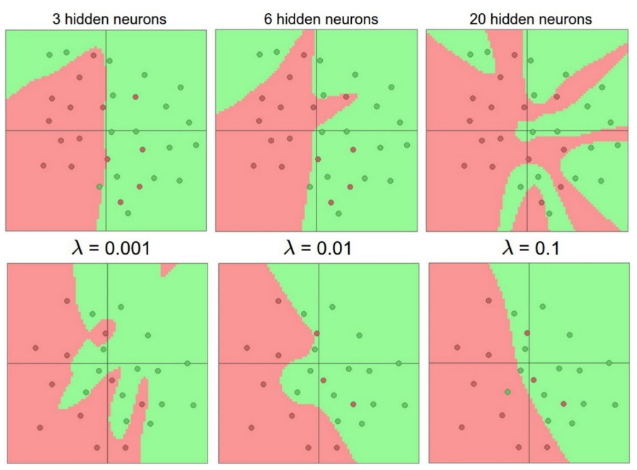
\includegraphics[width=0.5\textwidth]{images/overF.png}
    \caption{Trying different hyperparameters}
    \label{fig:overF}
\end{figure}





\chapter{Convolutional Neural Networks (CNNs)}
Convolutional neural network are built on the foundamental principles of the ordinary MLPs, indeed both:
\begin{compactitemize}
    \item Are composed of neurons with learnable weights and biases.
    \item Receive inputs, perform dot products and often are follow it with a non-linearity activation function.
    \item Have the parameters organized in layers, end the entire network represent a single, differentiable function, crucial for the training via backpropagation.
\end{compactitemize}

\section{The parameter explosion problem in MLPs and the solution with CNNs}
When we use a MLP to process images, we have to flatten the image into a vector, and then feed it to the network. This approach increase the number of parameters dramatically.
\begin{examplebox}
    A small 32x32 pixel color image (32x32x3=3,072 input features) connected to a 512-neuron hidden layer would need over 1.5 million weights for that single layer! This is computationally expensive and prone to overfitting.
\end{examplebox}
Another two big problem of MLPs are:
\begin{compactitemize}
    \item \textbf{Loss of Spatial Information:} MLPs require flattening the image, into 1D vector. This process discards the spatial relationships between pixels, it fortgets that pixel are arranged in a grid.
    \item \textbf{Inability to Learn Hierarchies:} These networks struggle to recognize that features are built hierarchically. For example, pixel from edges, edges combine into shapes, adn shapes from objects.
\end{compactitemize}

CNNs are specifically designed for image inputs.
Their main purpose is to automatically and adaptively learn spatial hierarchies of features.
They achieve this by detecting simple patterns in early layers and building upon them to
recognize more complex patterns in deeper layers.

\begin{infobox}[Inspiration from Biology: The Visual Cortex]
    The brain’s visual cortex processes information in stages. 
    Neurons in early stages detect simple features like edges, lines, and colors. 
    Later stages combine these simple patterns to recognize more complex elements like textures, shapes, and eventually entire objects. 
    Crucially, individual neurons only respond to stimuli in a small, localized region of our visual field. 
    This biological principle inspires the efficiency and scalability of CNNs.
\end{infobox}
    
\section{Architecture}
 A CNN is composed of a series of layers, each with a specific function:
\begin{compactitemize}
   \item \textbf{Convolutional Layers}
   \item \textbf{Activation Functions}
   \item \textbf{Pooling Layers}
   \item \textbf{Fully Connected Layers}
\end{compactitemize}

\begin{figure}[H]
    \centering
    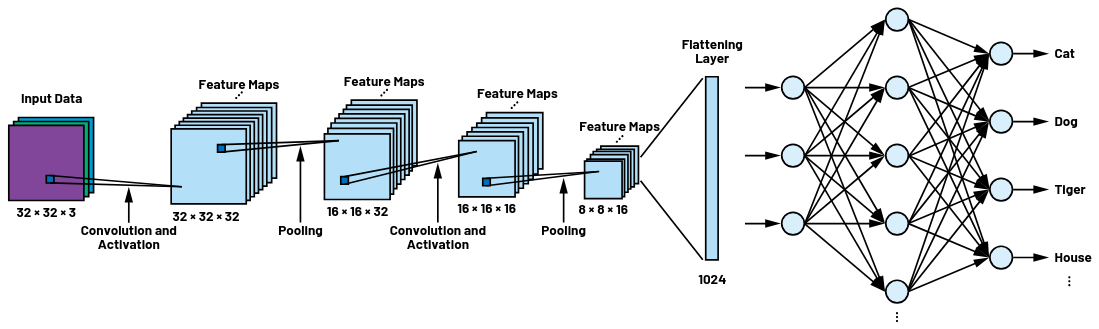
\includegraphics[width=1\textwidth]{images/CNN.png}
    \caption{Typical architecture of a Convolutional Neural Network (CNN).}
    \label{fig:cnn_architecture}
\end{figure}
Let's break down each component:
\begin{compactitemize}
    \item \textbf{The input:} The input to a CNN is typically a multi-channel image (e.g., RGB image with three channels). It is important to note that CNNs can also process other types of data, such as time series or 3D data, by adapting the convolutional operations accordingly.
    \item \textbf{Convolutional Layers:} These layers apply a set of learnable filters (or kernels) to the input image. Each filter slides over the input, performing a dot product between the filter and the local region of the input it covers. This operation produces a feature map that highlights specific patterns in the input, such as edges or textures. The filters are learned during training, allowing the network to adapt to the data.
    \item \textbf{Activation Functions:} After each convolutional operation, an activation function is applied to introduce non-linearity into the model. Common choices include ReLU (Rectified Linear Unit),sigmoid or tanh.
    \item \textbf{Pooling Layers:} These layers reduce the spatial dimensions of the feature maps, which helps to decrease the computational load and control overfitting. Common pooling operations include max pooling (which takes the maximum value in a local region) and average pooling (which computes the average value).
    \item \textbf{Fully Connected Layers:} After several convolutional and pooling layers, the high-level features are flattened into a 1D vector and passed through one or more fully connected layers. These layers function similarly to those in traditional MLPs, where each neuron is connected to every neuron in the previous layer. The final fully connected layer typically uses a softmax activation function for multi-class classification tasks.
\end{compactitemize}

\begin{infobox}[Important note]
    In the classic MLPs the feature extraction and the classification are both performed by the linear layers, while in CNNs the feature extraction is performed by the convolutional and pooling layers, and the classification is performed by the fully connected layers. It also important to note that like in MLPs, the firt layers was bigger and the last layer was smaller, in the first convolutional layer we tend to have more filters, while in the last convolutional layer we tend to have less filters. This is valid also for the spatioal dimensions, in the first convolutional layer we tend to have a bigger spatial dimension, while in the last convolutional layer we tend to have a smaller spatial dimension. This is made beacuse we want give in input to the fully connected layers a small number of features possible.
\end{infobox}

\section{Convolutional Layers}
Identically to the MLPs what a neuron does is a simple weighted sum of its input plus a bias:
\[
y = \sum_{i=1}^{n} w_i x_i + b
\]

\begin{tcolorbox}[
    colback=white,    % sfondo bianco (puoi anche mettere "colback=none")
    colframe=white,   % bordo invisibile
    boxrule=0pt,      % spessore bordo = 0
    arc=0pt,          % angoli non arrotondati (opzionale)
    left=0pt, right=0pt, top=0pt, bottom=0pt, % nessun margine interno extra
    enlarge left by=0mm, enlarge right by=0mm % allineamento perfetto
]
\begin{minipage}{0.65\textwidth}
However, a key difference in convolutional layers is that neurons are only \textbf{locally connected} to a small contiguous region of the input volume. 
This small region that each neuron "sees" of the previous layer is called the \textbf{receptive field} of the neuron. 
The size of the receptive field increases with the depth of the network: as we go deeper in the network, each neuron will see a larger portion of the input image, even if the size of the kernel remains the same.
\end{minipage}\hfill
\begin{minipage}{0.3\textwidth}
\centering
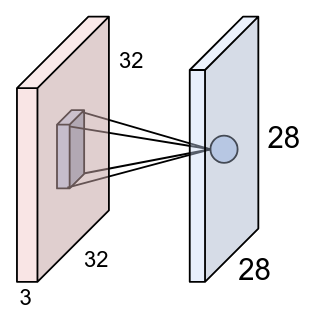
\includegraphics[width=\linewidth]{images/local_connettivity.png}
\captionof{figure}{Local connectivity in CNNs.}
\end{minipage}
\end{tcolorbox}

\begin{infobox}[Intuition of parameter sharing]
    Intuition: If a feature (e.g., an edge or a specific texture) is useful to detect at one spatial
    location in an image, it’s likely useful to detect it at other locations too.
    To leverage this, we constrain all neurons within a single depth slice (i.e., those producing a
    single feature map) to share the same set of weights and bias.
    This parameter sharing allows the forward pass of a convolutional layer to be computed as a
    convolution operation. Each set of shared weights is often referred to as a filter or kernel
    that scans across the entire input volume.
\end{infobox}

Suppose that one kernel catch a specific feature, we may use more kernel to catch more features, so we can have multiple filters in a convolutional layer. In particular during the forward pass:

\begin{compactitemize}
    \item Each filter is \textbf{convolved} with the input volume.
    \item This operation produces a 2D output, called a \textbf{feature map} or \textbf{activation map}.
    \item A distinc feature map is generated for each filter.
\end{compactitemize}
The output volume of a convolutional layer is obtained by stacking the feature maps produced by each filter along the depth dimension.

\begin{figure}[H]
    \centering
    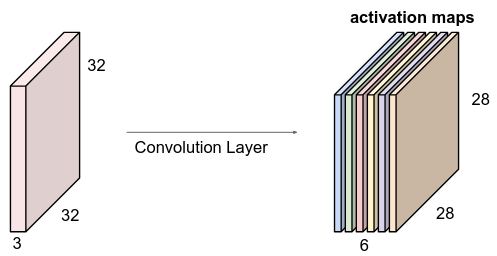
\includegraphics[width=0.45\textwidth]{images/CNN_layer.png}
    \caption{Convolutional layer with multiple filters producing multiple feature maps.}
    \label{fig:cnn_multiple_filters}
\end{figure}
When we talk about a kernel size, we reffere always to the spatial dimensions of the kernel, so a kernel size of 3x3 means that the kernel has a height and width of 3 pixels each. The depth of the kernel is always equal to the depth of the input volume. So for example with a input 5x5x3 the parameter to learn are 75 not 25.

\subsection{What is the convolution operation?}
The convolution operation is a mathematical operation that combines two functions to produce a third function. In the context of CNNs, it involves sliding a filter (or kernel) over the input image and computing the dot product between the filter and the local region of the input it covers. This operation is repeated across the entire input image to produce a feature map.
The convolution operation can be mathematically expressed as:
\[
S(i, j) = (I * K)(i, j) = \sum_{m} \sum_{n} I(i+m, j+n) K(m, n)
\]
Where:
\begin{compactitemize}
    \item \(S(i, j)\) is the output feature map at position \((i, j)\).
    \item \(I\) is the input image.
    \item \(K\) is the filter (or kernel).
    \item \(m\) and \(n\) are the dimensions of the filter.
\end{compactitemize}
\begin{figure}[H]
    \centering
    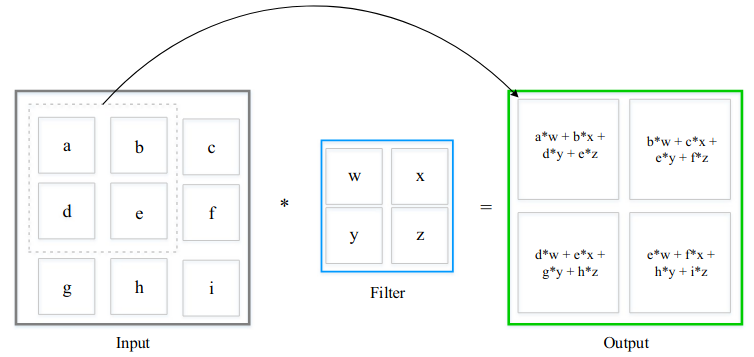
\includegraphics[width=0.8\textwidth]{images/convolution.png}
    \caption{Convolution operation example.}
    \label{fig:convolution_operation}
\end{figure}
\textbf{Note:} that this diagram simplifies the proccess for a single channel. In reality, a filter's depth must match the input volume's depth (e.g., a 3x3x\textbf{3} filter fot a 32x32x\textbf{3} input image). The convolution involves element-wise multiplication across all channels, and the result are summed up, along with a bias term, to produce a single value in the output feature map.

\subsection{Hyperparameters of Convolutional Layers}
Each convolutional layer is defined by the following hyperparameters:
\begin{compactitemize}
    \item \textbf{Number of Filters ($C_{\text{out}}$)}: Determines the depth of the output volume (i.e., how many feature maps are produced).
    \item \textbf{Kernel Size ($K \times K$)}: The spatial dimensions of the convolutional filters. These are typically square. Each filter also extends through the full depth ($C_{\text{in}}$) of the input volume.
    \item \textbf{Stride ($S$)}: The number of pixels the convolutional filter shifts across the input at each step. A larger stride results in a smaller output volume.
\end{compactitemize}
Additionally, the presence and amount of \textbf{Spatial Padding ($P$)} applied to the input volume can be considered another hyperparameter. Padding is often used to preserve spatial dimensions or to ensure an integer output size.

\begin{infobox}[Different Types of Padding]
    When we talk about padding, the first question that arises is: with which value should we pad the input? The most common choice is to pad with zeros, a technique called \textbf{zero-padding}. Zero-padding is simple and computationally efficient, and it allows us to control the spatial dimensions of the output volume. However, it can also introduce some artifacts: the artificial addition of zeros creates "black regions" along the borders of the feature maps, which do not represent any real information from the input. These regions can sometimes bias the network, especially in early layers, causing the convolutional filters to respond differently near the edges compared to the center of the input.  
    
    To mitigate these issues, other padding strategies can be used. \textbf{One-padding} consists of filling the padded areas with ones instead of zeros. This can reduce the stark contrast created by zeros, but it may still introduce artificial patterns that the network could misinterpret. Another approach is \textbf{mirror-padding}, also called \textbf{reflect-padding}, where the border values of the input are mirrored to extend the input volume. This technique helps preserve the local structures and patterns at the edges, minimizing artificial bias while still allowing control over output dimensions. Each padding strategy has its trade-offs, and the choice often depends on the type of data and the specific architecture being used.
\end{infobox}

\subsection{Number of Learnable Parameters}
Given an input volume of size \(H_{\text{in}} \times W_{\text{in}} \times C_{\text{in}}\) and a convolutional layer with \(C_{\text{out}}\) filters of size \(K \times K\), the number of learnable parameters in the convolutional layer can be calculated as follows:
\[
\text{Number of Parameters} = (K \times K \times C_{\text{in}} + 1) \times C_{\text{out}}
\]
Where:
\begin{compactitemize}
    \item \(K \times K \times C_{\text{in}}\) is the number of weights per filter (the filter size times the depth of the input volume).
    \item The "+1" accounts for the bias term associated with each filter.
    \item \(C_{\text{out}}\) is the number of filters in the convolutional layer.
\end{compactitemize}

\begin{figure}[H]
    \centering
    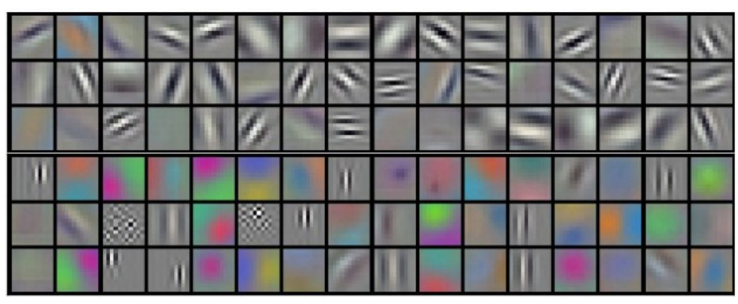
\includegraphics[width=0.8\textwidth]{images/filter_example.png}
    \caption{Examples of learned weight from the first convolutional layer.}
    \label{fig:cnn_learned_weights}
\end{figure}

Each of the 96 filters shown here is of size 11 × 11 × 3. This visualization confirms that the
parameter sharing assumption is highly reasonable: if detecting a feature like a horizontal edge
is important at one location in an image, it’s intuitively useful at other locations as well,
contributing to the \textbf{translational invariance} of CNNs.

\subsection{Activation Functions}
Activation functions introduce critical non-linearity into the network by performing an element-wise operation on the input volume. The most common ones include:

\begin{figure}[H]
    \centering
    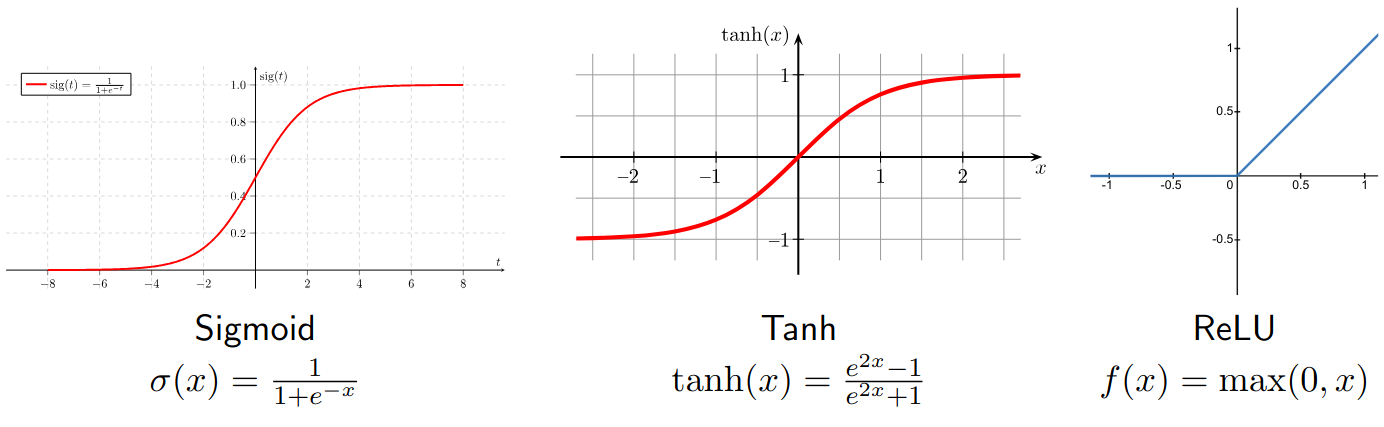
\includegraphics[width=1\textwidth]{images/activation_function.png}
    \caption{Most common activation functions used in CNNs.}
    \label{fig: activation_functions}
\end{figure}
It's worth noting that more advances activation functions have also been developed.

Among these activation function the most widely used is the relu, this is because:
\begin{compactitemize}
    \item \textbf{Accelerated Convergence:} ReLU was empirically found to greatly accelerate the convergence of SGD compared to sigmoid/tanh in many scenarios.
    \item \textbf{Computational Efficiency:} ReLU can be implemented by a simple thresholding operation ($f(x)=max(0,x)$), wheread Sigmoid and Tanh involve more complex exponential calculations.
\end{compactitemize}

Follow is shown a visulizating activation maps from different CNN stages (layer). To show the network's area focus, each map is upsampled to match the original image's dimension.
\begin{figure}[H]
    \centering
    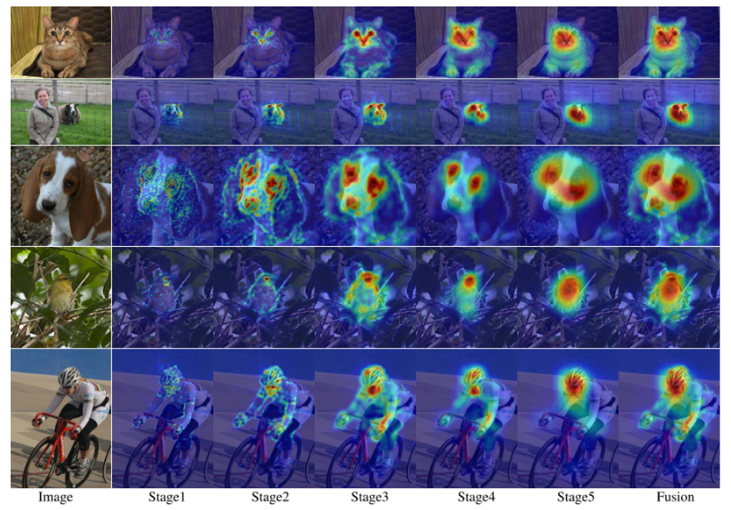
\includegraphics[width=0.6\textwidth]{images/stage.png}
    \caption{Activation maps from different CNN stages.}
    \label{fig: cnn_stages}
\end{figure}

\section{Pooling Layers}
Pooling layers are used to reduce the spatial dimensions (height and width) of the input volume, while retaining the most important information. This downsampling helps to decrease the computational load, control overfitting, and make the network more robust to small translations in the input.
\begin{figure}[H]
    \centering
    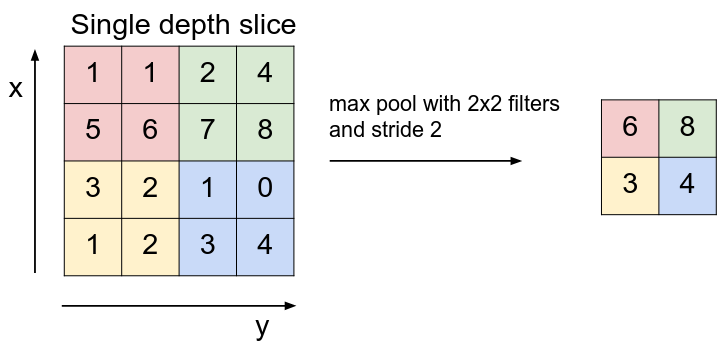
\includegraphics[width=0.5\textwidth]{images/max_pooling.png}
    \caption{Max pooling operation example.}
    \label{fig:max_pooling_operation}
\end{figure}

Key hyperparameters of pooling layers include:
\begin{compactitemize}
    \item \textbf{Pool Size ($P \times P$)}: The spatial dimensions of the pooling window. Common choices are 2x2 or 3x3.
    \item \textbf{Stride ($S$)}: The number of pixels the pooling window shifts across the input at each step. A larger stride results in a smaller output volume. When $S=K$, the pooling windows do not overlap.
\end{compactitemize}

The type of \textbf{pooling function} used is an addition to hyperparameter. While many aggregation functions are possible, the mosto common in practice are:
\begin{compactitemize}
    \item \textbf{Max Pooling:} Takes the maximum value within the pooling window. This operation is effective at capturing the most prominent features and is widely used in practice.
    \item \textbf{Average Pooling:} Computes the average value within the pooling window. This approach provides a smoother representation of the features but may dilute strong activations.
\end{compactitemize}

\begin{infobox}[Typical Pooling Configuration]
    The tipically configuration of a pooling layer is a 2x2 max pooling with stride 2. In this setting, $75$ of input volume activation are discarded.
\end{infobox}

\begin{infobox}[Pooling layer cons]
    While beneficial for some tasks, the aggressive downsampling of pooling layers can lead to a loss of spatial information, which may be detrimental for tasks requiring precise localization, such as image segmentation. Additionally, pooling operations are not learnable, meaning they do not adapt to the data during training. This limitation has led to the exploration of alternative downsampling methods, such as strided convolutions or adaptive pooling techniques, which can provide more flexibility and potentially better performance in certain applications.
\end{infobox}

\begin{figure}[H]
    \centering
    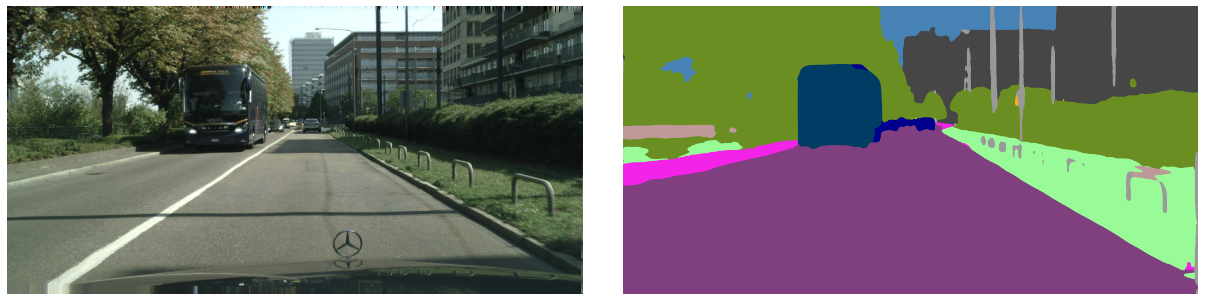
\includegraphics[width=0.9\textwidth]{images/loss_spatial.png}
    \caption{Loss of spatial information due to pooling.}
    \label{fig:loss_spatial_info}
\end{figure}

\subsection{Computing Output Volume Size}
Initially, let's define the variables:
\begin{compactitemize}
    \item \(H_{\text{in}}\): Height of the input volume.
    \item \(W_{\text{in}}\): Width of the input volume.
    \item \(C_{\text{in}}\): Depth (number of channels) of the input volume.
    \item \(C_{\text{out}}\): Number of filters (depth of the output volume).
    \item \(K\): Kernel size
    \item \(S\): Stride 
    \item \(P\): Padding
\end{compactitemize}

For a \textbf{convolutional layer}, given an input volume of size \(H_{\text{in}} \times W_{\text{in}} \times C_{\text{in}}\), the output volume size can be computed as follows:
\[
H_{\text{out}} = \frac{H_{\text{in}} - K + 2P}{S} + 1
\]
\[
W_{\text{out}} = \frac{W_{\text{in}} - K + 2P}{S} + 1
\]
\[
C_{\text{out}} = \text{Number of filters}
\]

For a \textbf{pooling layer}, given an input volume of size \(H_{\text{in}} \times W_{\text{in}} \times C_{\text{in}}\), the output volume size can be computed as follows:
\[
H_{\text{out}} = \frac{H_{\text{in}} - P}{S} + 1
\]
\[
W_{\text{out}} = \frac{W_{\text{in}} - P}{S} + 1
\]
\[
C_{\text{out}} = C_{\text{in}}
\]

For an \textbf{activation layer}, the output volume size remains the same as the input volume size:
\[
H_{\text{out}} = H_{\text{in}}
\]
\[
W_{\text{out}} = W_{\text{in}}
\]
\[
C_{\text{out}} = C_{\text{in}}
\]
This is because activation functions are applied element-wise and do not change the spatial dimensions or depth of the volume.

\section{Real Implementation of CNNs}

\subsection{LeNet}
The architecture known as \textbf{LeNet} was introduced in one of the pioneering works on Convolutional Neural Networks (CNNs), laying much of the groundwork for modern deep learning approaches. It demonstrated the \textbf{efficacy of CNNs for handwritten digit recognition} through an end-to-end trainable design. The network processes \textbf{32×32 pixel input images} through successive layers of convolution and subsampling, where each convolutional layer employs \textbf{learnable filters (5×5 kernels)} to extract spatial features. The subsampling layers, using \textbf{average pooling over 2×2 windows with stride 2}, progressively reduce spatial resolution while preserving essential information. Non-linear transformations are introduced through \textbf{sigmoid activation functions}, whose coefficients and biases control the non-linearity of each unit. This architecture alternates convolutional and subsampling layers, forming a bi-pyramidal structure in which the \textbf{number of feature maps increases as spatial resolution decreases}. Overall, LeNet represented one of the first \textbf{complete, trainable CNN architectures}, setting the foundation for subsequent developments in deep learning.
\begin{figure}[H]
    \centering
    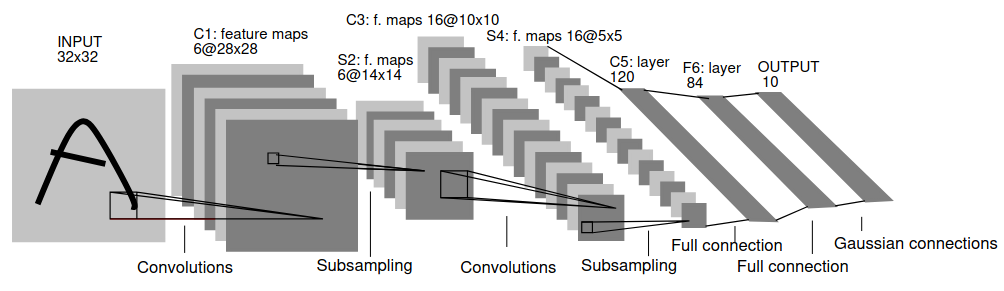
\includegraphics[width=0.9\textwidth]{images/LeNet.png}
    \caption{LeNet architecture.}
    \label{fig:lenet_architecture}
\end{figure}

\subsection{AlexNet}
\textbf{AlexNet}, introduced in 2012, marked a major breakthrough in image recognition by winning the \textbf{ImageNet Large Scale Visual Recognition Challenge} with a significant margin, demonstrating the unprecedented power of \textbf{Convolutional Neural Networks (CNNs)} at scale. The architecture consisted of \textbf{eight layers with learnable parameters}, including five convolutional and three fully connected layers, processing high-dimensional image inputs. The network employed a \textbf{large first kernel (11×11)} in its initial convolutional layer, enabling the capture of broader spatial context. Moreover, AlexNet \textbf{pioneered the use of Rectified Linear Units (ReLU)} as activation functions, which significantly accelerated training compared to traditional sigmoidal activations. Another key innovation was the \textbf{parallel training across two GPUs}, allowing the model to handle an unprecedented number of parameters for its time, with limited inter-GPU communication at specific layers. Overall, AlexNet established the foundation for the deep learning revolution in computer vision.
\begin{figure}[H]
    \centering
    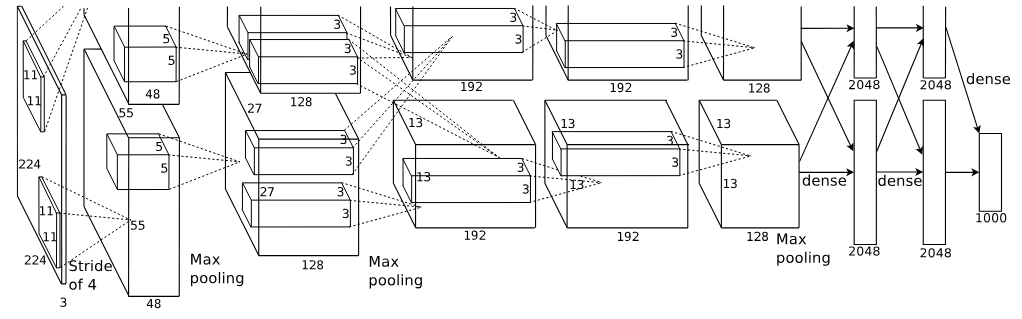
\includegraphics[width=0.9\textwidth]{images/AlexNet.png}
    \caption{AlexNet architecture.}
    \label{fig:alexnet_architecture}
\end{figure}

\subsection{VGGNet}
\textbf{VGG}, introduced in 2014 by the \textbf{Oxford Visual Geometry Group (VGG)}, represents a family of deep convolutional neural networks that achieved remarkable success in large-scale image recognition tasks. It became widely recognized for its \textbf{simplicity, effectiveness, and influence} on subsequent network designs. The model \textbf{secured 1st and 2nd places} in the ImageNet 2014 localization and classification challenges, establishing a new standard for deep learning architectures.  
\begin{compactitemize}
    \item \textbf{Input:} Fixed-size \(224 \times 224\) RGB images, mean-subtracted during pre-processing.  
    \item \textbf{Architecture:} Consists of 16 weight layers (\textbf{VGG16}), including 13 convolutional and 3 fully connected layers.  
    \item \textbf{Convolutional Filters:} Employs small and uniform \textbf{3×3 kernels} with stride 1, stacked to increase non-linearity and capture complex patterns effectively.  
    \item \textbf{Activation Function:} Each convolutional and fully connected layer is followed by a \textbf{ReLU} activation function.  
    \item \textbf{Spatial Pooling:} Includes five \textbf{max-pooling layers} using 2×2 windows with stride 2 for progressive spatial downsampling.  
    \item \textbf{Fully Connected Layers:} The last three layers are fully connected, with the first two containing \textbf{4096 neurons} each and the final one having \textbf{1000 neurons} for classification, followed by a \textbf{Softmax} activation.  
    \item \textbf{Pre-trained Weights:} Released publicly, enabling \textbf{transfer learning} and establishing VGG as a popular backbone for diverse computer vision tasks.    
\end{compactitemize}
\begin{figure}[H]
    \centering
    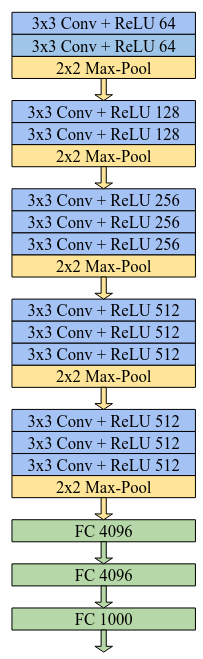
\includegraphics[height=0.4\textheight,keepaspectratio]{images/VGG.png}
    \label{fig:forecast_prediction}
\end{figure}

The net contains approximately \textbf{138 million learnable parameters}, with about \textbf{70\% located in the fully connected layers}. Notably, a single fully connected layer is responsible for roughly \textbf{100 million parameters}.
\begin{figure}[H]
    \centering
    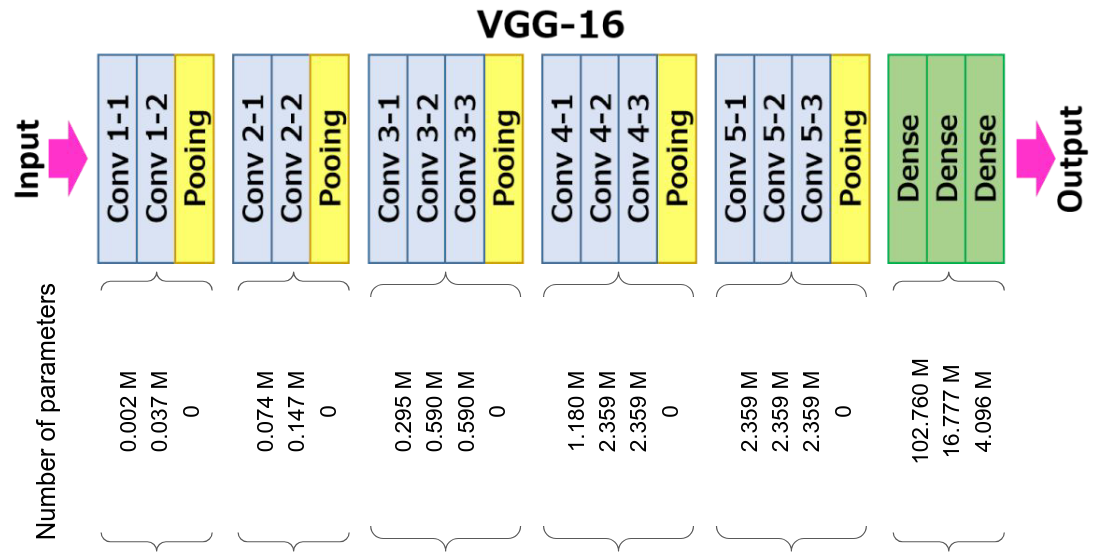
\includegraphics[width=0.7\textwidth]{images/number_parameters.png}
    \caption{Number of parameters in VGG16.}
    \label{fig:vgg_number_parameters}
\end{figure}
In traditional convolutional neural networks, simply \textbf{stacking more layers beyond a certain depth} often leads to \textbf{performance degradation} rather than improvement. This phenomenon is \textbf{not caused by overfitting}, as deeper models exhibit \textbf{higher training and test error}. A key hypothesized reason is the \textbf{difficulty of training deep layers to approximate simple identity mappings}. Additionally, very deep networks suffer from the problem of \textbf{vanishing or exploding gradients}, where gradients propagated backward through many layers become either extremely small (\textbf{vanishing}) or extremely large (\textbf{exploding}). This instability severely \textbf{hinders the ability of early layers to learn effectively}, making it challenging to train very deep architectures.

\subsection{The state of the art: The Residual Neural Network (ResNet)}
\textbf{ResNet (Residual Networks)}, introduced in 2015, was a groundbreaking architecture that won both the \textbf{ImageNet Large Scale Visual Recognition Challenge (ILSVRC 2015)} and \textbf{COCO 2015} for detection, segmentation, and localization. ResNet addressed the critical problem of training very deep convolutional networks, which often suffered from performance degradation due to \textbf{vanishing or exploding gradients}.  
\begin{figure}[H]
    \centering
    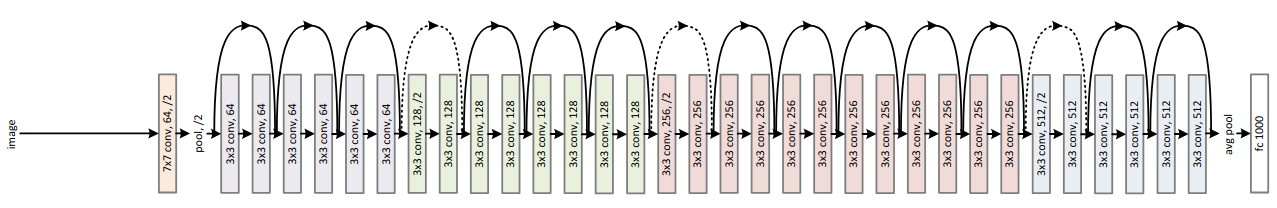
\includegraphics[width=1\textwidth]{images/ResNet.png}
    \caption{ResNet architecture.}
    \label{fig:resnet_architecture}
\end{figure}
\begin{compactitemize}
    \item \textbf{Input:} Accepts \(224 \times 224\) RGB images.
    \item \textbf{Architecture:} Features \textbf{ultra-deep networks}, with common variants including \textbf{ResNet-50, ResNet-101, and ResNet-152}, reaching up to 152 layers, far deeper than VGG.  
    \item \textbf{Output:} Produces predictions for \textbf{1000 ImageNet classes}.  
    \item \textbf{Key Innovation – Residual Learning:} Instead of directly learning the underlying mapping \(H(x)\), the network learns the \textbf{residual function} \(F(x)\) such that:
    \[
    H(x) = F(x) + x
    \]
    This formulation allows layers to focus on learning the difference (residual) between the desired output and the input, making optimization easier.  
    \item \textbf{Residual Block:} The fundamental building block of ResNet, implemented via \textbf{skip connections}:
    \begin{itemize}
        \item The input \(x\) is added directly to the output of the residual function \(F(x)\).  
        \item \textbf{Easier gradient flow:} Skip connections allow gradients to bypass intermediate layers, mitigating vanishing/exploding gradient problems.  
        \item Supports much deeper networks without performance degradation.  
    \end{itemize}
    \begin{figure}[H]
        \centering
        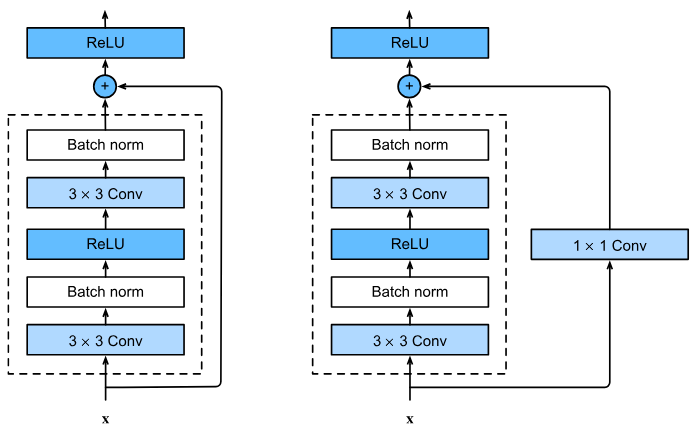
\includegraphics[width=0.5\textwidth]{images/residual_block.png}
        \caption{Residual Block.}
        \label{fig:residual_block}
    \end{figure}
    \item \textbf{Impact and Advantages:}
    \begin{itemize}
        \item \textbf{Enabled ultra-deep networks:} Training models with unprecedented depth (e.g., 152 layers) became feasible.  
        \item \textbf{Improved performance:} Achieved state-of-the-art results across numerous computer vision tasks, including image classification, detection, and segmentation.  
        \item \textbf{Simplified training:} Residual connections reduce optimization difficulty, preventing the degradation problem observed in traditional deep networks.  
        \item \textbf{Foundation for future architectures:} The concept of \textbf{skip connections} and residual learning influenced many subsequent CNN architectures and even modern Transformer models.  
    \end{itemize}
\end{compactitemize}

\section{Batch Normalization}
In deep neural networks with many layers, the distribution of inputs to each layer tends to change continuously during training as the parameters of the preceding layers are updated. This phenomenon is known as \textbf{Internal Covariate Shift}. It occurs because every time the weights in earlier layers are modified, the statistical properties (mean and variance) of the inputs received by deeper layers also change. As a result, each layer must constantly adapt to a shifting input distribution, which \textbf{slows down training} and makes it more difficult for the network to converge effectively. Small parameter changes in the early layers can become amplified as they propagate forward through the network, leading to instability and poor optimization efficiency.  
\begin{figure}[H]
    \centering
    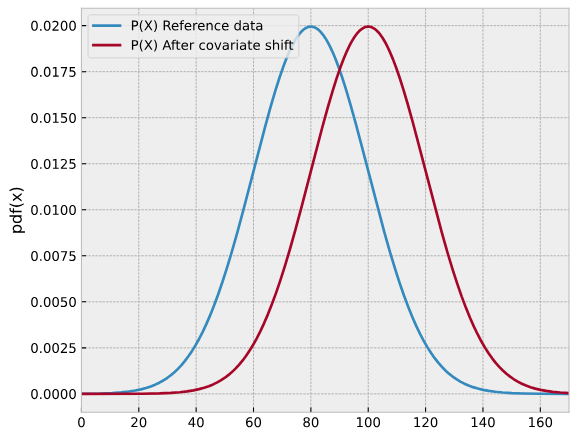
\includegraphics[width=0.5\textwidth]{images/covariance_shift.png}
    \caption{Internal covariance shift.}
    \label{fig:internal_covariance_shift}
\end{figure}
To address this issue, \textbf{Batch Normalization (BN)} was introduced in the paper \textit{"Batch Normalization: Accelerating Deep Network Training by Reducing Internal Covariate Shift"} by Ioffe and Szegedy (2015). Batch Normalization standardizes the inputs to each layer within a mini-batch by re-centering and rescaling them to have zero mean and unit variance, followed by a learnable shift and scale transformation. This normalization \textbf{stabilizes the learning process}, allowing higher learning rates, faster convergence, and reduced sensitivity to weight initialization. By mitigating internal covariate shift, Batch Normalization made the training of very deep networks significantly more stable and efficient, becoming a fundamental component of modern deep learning architectures.

\subsection{How Batch Normalization Works During Training}
During training, Batch Normalization operates on mini-batches of data to normalize the inputs to each layer. The process involves the following steps for each mini-batch:
\begin{compactitemize}
    \item \textbf{Compute Batch Statistics:} For each feature in the mini-batch, calculate the mean (\(\mu_B\)) and variance (\(\sigma_B^2\)):
    \[
    \mu_B = \frac{1}{m} \sum_{i=1}^{m} x_i
    \]
    \[
    \sigma_B^2 = \frac{1}{m} \sum_{i=1}^{m} (x_i - \mu_B)^2
    \]
    where \(m\) is the number of examples in the mini-batch, and \(x_i\) represents the input features.
    \item \textbf{Normalize the Inputs:} Each input feature is normalized using the computed mean and variance:
    \[
    \hat{x}_i = \frac{x_i - \mu_B}{\sqrt{\sigma_B^2 + \epsilon}}
    \]
    where \(\epsilon\) is a small constant added for numerical stability.
    \item \textbf{Scale and Shift:} The normalized inputs are then scaled and shifted using learnable parameters \(\gamma\) (scale) and \(\beta\) (shift):
    \[
    y_i = \gamma \hat{x}_i + \beta
    \]
    This allows the network to learn an optimal representation of the data after normalization.
\end{compactitemize}
After normalizing, the activations have a mean of 0 and a standard deviation of 1. This might be too restrictive for the network. To address this, Batch Normalization introduces two learnable parameters per feature: a scaling factor \(\gamma\) and a shifting factor \(\beta\). These parameters allow the network to adjust the normalized output, enabling it to recover the original distribution if necessary. By learning these parameters, the network can maintain its expressive power while benefiting from the stability provided by normalization.

\subsection{How Batch Normalization Works During Inference}
During inference (testing or deployment), the behavior of Batch Normalization differs from training. Instead of using the statistics computed from the current mini-batch, Batch Normalization relies on \textbf{running estimates} of the mean and variance that were accumulated during training. The steps are as follows:
\begin{compactitemize}
    \item \textbf{Use Running Estimates:} Instead of calculating the mean and variance from the current mini-batch, use the running estimates \(\mu_{\text{running}}\) and \(\sigma_{\text{running}}^2\) that were updated during training.
    \item \textbf{Normalize the Inputs:} Each input feature is normalized using the running estimates:
    \[
    \hat{x}_i = \frac{x_i - \mu_{\text{running}}}{\sqrt{\sigma_{\text{running}}^2 + \epsilon}}
    \]
    \item \textbf{Scale and Shift:} The normalized inputs are then scaled and shifted using the learned parameters \(\gamma\) and \(\beta\):
    \[
    y_i = \gamma \hat{x}_i + \beta
    \]
\end{compactitemize}
This approach ensures that the model's predictions are consistent and stable during inference, as they are based on the overall data distribution learned during training rather than the potentially noisy statistics of a single mini-batch.

\subsection{Benefits of Batch Normalization}
Batch Normalization offers several significant benefits that enhance the training and performance of deep neural networks:
\begin{compactitemize}
    \item \textbf{Faster Training:} Allows for higher learning rates, leading to quicker convergence and reduced training time.
    \item \textbf{Reduces Internal Covariate Shift:} Stabilizes the distribution of layer inputs, making the training process more stable.
    \item \textbf{Regularization Effect:} The noise from mini-batch statistics has a slight regularizing effect, sometimes reducing the need for dropout.
    \item \textbf{Less Sensitive to Inizialization:} Makes the network less dependent on the initial weights.
\end{compactitemize}
\chapter{Recurrent Neural Networks}

\section{Introduction to Time Series}
A time series is a set of observations $\{x_t\}_{t \in \tau}$ collected over time. Based in the nature of $\tau$ we can distinguish between:
\begin{compactitemize}
    \item \textbf{Continuous time series}, when observation are made continuosly.
    \item \textbf{Discrete time series}, when the set of observation is finite. If the time delta between data points is fixed, the series is said to be regularly sampled with sampling frequecy $f_c = \frac{1}{\Delta t}$.
\end{compactitemize}
\begin{figure}[H]
    \centering
    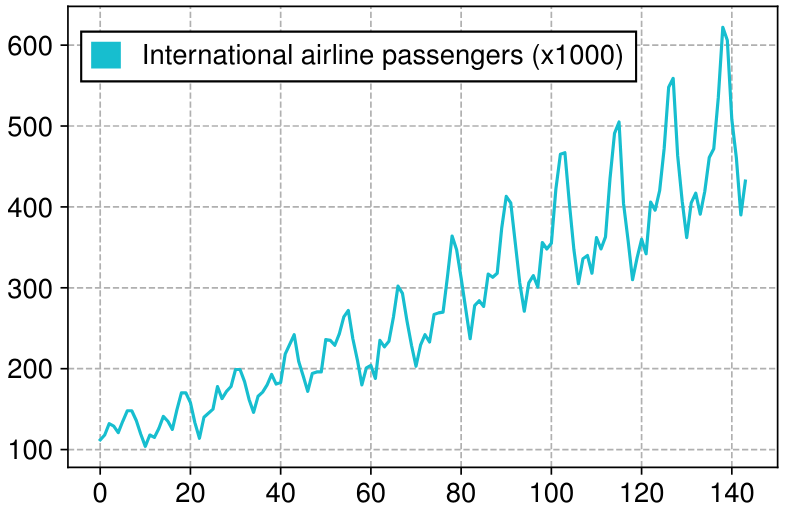
\includegraphics[width=0.6\textwidth]{images/series.png}
    \caption{Example of discrete and regulary sampled time series.}
    \label{fig:series}
\end{figure}
\begin{infobox}[Most important features of a time series]
    One important thing to note about the image above is that the series is composed of two characteristics: it increases over time and it oscillates. 
    If we focus on these aspects, we can notice that its behavior is periodic, and we can identify some important features:
    \begin{compactitemize}
        \item \textbf{Trend}: tendency of the series to increase or decrease over time.
        \item \textbf{Seasonality}: regular fluctuations that is more or less stable for each period of reference (e.g., daily, monthly, yearly).
        \item \textbf{Cyclic patterns}: periodic fluctuations around the trend.
        \item \textbf{Outliers}: values that appear out-of-distribution with respect to the rest of data.
        \item \textbf{Stationarity}: a stationary time series has statistical properties (mean, variance) that do not change over time. An example of a stationary series is a cosine or sine function.
    \end{compactitemize}
\end{infobox}

\subsection{STL Decomposition}
The \textbf{STL} decomosition split data into \textbf{S}easonality and \textbf{T}rend components using the \textbf{L}oess regression. The presence of a trend rules out the possibility that the series is stationary.
\begin{figure}[H]
    \centering
    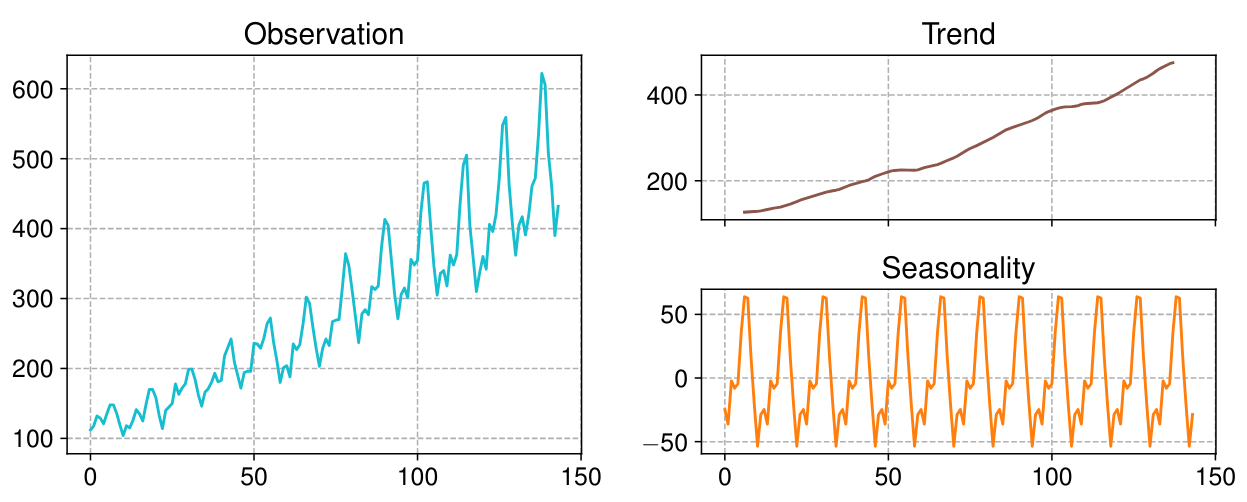
\includegraphics[width=0.9\textwidth]{images/STL_decomposition.png}
    \caption{Example of STL decomosition.}
    \label{fig:STL_decomosition}
\end{figure}

\begin{infobox}[Considerations]
    In this example, trend and seasonality components capture most of the patterns in the series. Noise and irregularities that cannot be decomposed are called \textbf{residuals} or \textbf{noise}. The residual is the difference between the original series and the sum of trend and seasonality (see Figure \ref{fig:Residuals}).
\end{infobox}
\begin{figure}[H]
    \centering
    \begin{minipage}{0.45\textwidth}
        \centering
        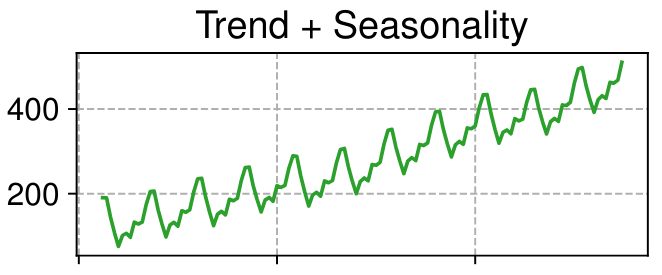
\includegraphics[width=\textwidth]{images/TS.png}
        \caption{Trend + Seasonality}
        \label{fig:Trend_Seasonality}
    \end{minipage}
    \hfill
    \begin{minipage}{0.45\textwidth}
        \centering
        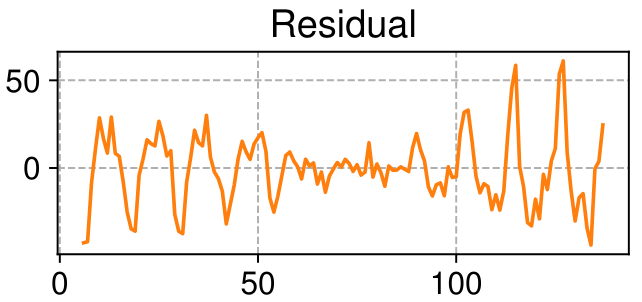
\includegraphics[width=\textwidth]{images/residual.png}
        \caption{Residuals}
        \label{fig:Residuals}
    \end{minipage}
    \label{fig:TS_Residuals}
\end{figure}

\section{Forecasting}
Having observed a time series over a period $\tau$ we want to estimate a future value (\textbf{forecast}) $\hat{x}_{\tau + h}$ with $h>0$. The value $h$ is called \textbf{forecast horizon}. To do that we can use:
\begin{compactitemize}
    \item \textbf{Data Generating Process (DPG):} essentialy we knew the process that had generated the data, and so it easy to make prediction. Obviously this is not the case in real life.
    \item \textbf{Approximate DGP:} we can try to approximate the DGP with a model, and use it to make prediction. This is the most common approach.
\end{compactitemize}
\begin{figure}[H]
    \centering
    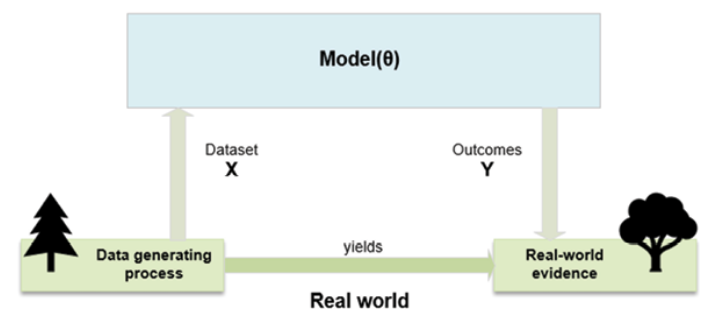
\includegraphics[width=0.7\textwidth]{images/forecasting.png}
    \caption{Idea of forecating should be.}
    \label{fig:forecasting}
\end{figure}

\begin{wrapfigure}{r}{0.35\textwidth}
    \centering
    \vspace{-10pt}
    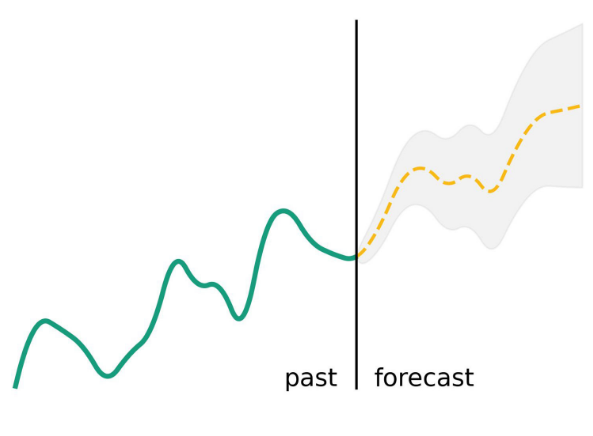
\includegraphics[width=\linewidth]{images/forecast_prediction.png}
    \caption{Example of forecast prediction.}
    \label{fig:forecast_prediction}
    \vspace{-10pt}
\end{wrapfigure}
Forecasting is used in many fields, such as:
\begin{compactitemize}
    \item \textbf{Finance:} Predict stock prices, bond yields, or currency exchange rates to guide investment strategies.
    \item \textbf{Retail:} Forecast demand to keep inventory levels optimal (avoid overstocking or stockouts).
    \item \textbf{Energy:} Predict eletricity load to balance grid supply and demand in real-time.
    \item \textbf{Words:} Predict the next word in a sentence for applications like text autocompletion and chatbots.
\end{compactitemize}

\subsection{Forecasting Problem}
Most forecasting models consider a limited window of past observations 
$\{x_t, x_{t-1}, \ldots, x_{t-q}\}$ and can be expressed as:
\[
x_t = f(x_{t-1}, \ldots, x_{t-q}; \boldsymbol{\phi}) 
    + g(\xi_{t-1}, \ldots, \xi_{t-q}; \boldsymbol{\theta})
\]

where $\xi_t, \ldots, \xi_{t-q}$ are random disturbances with mean $0$ and finite variance. 
The vectors $\boldsymbol{\phi}$ and $\boldsymbol{\theta}$ are the model parameters to be estimated.

The function $f(\cdot)$ captures the deterministic part of the model, describing how past observations influence the current value $x_t$. 
Conversely, the function $g(\cdot)$ introduces the stochastic component: 
since it depends on random noise terms $\xi_t$, it accounts for unpredictable fluctuations and uncertainty in the forecast. 
As a result, the prediction $\hat{x}_{\tau + h}$ is not purely deterministic, but inherently stochastic due to the influence of these random disturbances.
\begin{figure}[H]
    \centering
    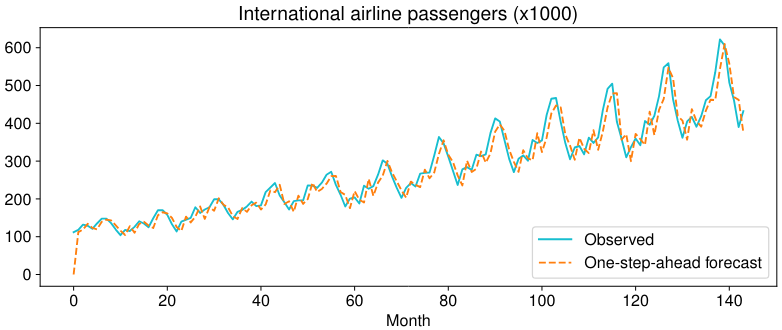
\includegraphics[width=0.85\textwidth]{images/F_problem.png}
    \caption{Another forecasting example.}
    \label{fig:forecasting}
\end{figure}

\subsection{Autoregressive Models}
An \textbf{autoregressive model} of order $p$, denoted as $\text{AR}(p)$, is defined as:
\[
x_t = \sum_{i=1}^{p} \phi_i x_{t-i} + \xi_t
\]
In this model, the current value $x_t$ is expressed as a linear combination of its $p$ most recent past values, plus a random disturbance term $\xi_t$.
\begin{compactitemize}
    \item The \textbf{order $p$} determines how many past observations are taken into account for the prediction. For example, an $\text{AR}(3)$ model depends on $x_{t-1}$, $x_{t-2}$, and $x_{t-3}$.
    \item The coefficients $\phi_i$ are the \textbf{learnable parameters} of the model, estimated from data to best capture the temporal dependencies.
    \item The term $\xi_t$ represents the \textbf{white noise}, i.e., random variations that are not explained by past values. It is typically modeled as a normal distribution:
    \[
    \xi_t \sim \mathcal{N}(0, \sigma^2)
    \]
    with mean $0$ and finite variance $\sigma^2$.
\end{compactitemize}
Thus, the autoregressive model captures the deterministic dependency of $x_t$ on its recent history through the parameters $\boldsymbol{\phi}$, while $\xi_t$ introduces the stochastic (random) component of the process.

\subsection{Moving Average Models}
A \textbf{moving average model} of order $q$, denoted as $\text{MA}(q)$, is defined as:
\[
x_t = \mu + \xi_t + \sum_{i=1}^{q} \theta_i \, \xi_{t-i}
\]
In this model, the current value $x_t$ is expressed as a linear combination of the last $q$ random shocks (or errors), plus the mean of the series.
\begin{compactitemize}
    \item The \textbf{order $q$} determines how many past random variations (errors) are taken into account. For example, an $\text{MA}(2)$ model depends on $\xi_{t-1}$ and $\xi_{t-2}$.
    \item The parameter $\mu$ represents the \textbf{mean level} of the time series, often estimated as the empirical mean of $\{x_t\}_{t \in \tau}$.
    \item The coefficients $\theta_i$ are the \textbf{learnable parameters} of the model, which determine how much influence each past error has on the current value.
    \item The terms $\xi_{t-i}$ represent the \textbf{previous random shocks} or error terms, typically modeled as white noise:
    \[
    \xi_t \sim \mathcal{N}(0, \sigma^2)
    \]
    with mean $0$ and finite variance $\sigma^2$.
\end{compactitemize}
Thus, the moving average model captures the stochastic dependency of $x_t$ on past random variations, rather than on past observed values. The process is therefore driven by recent shocks, weighted by the parameters $\boldsymbol{\theta}$.

\subsection{ARMA Models}
An \textbf{autoregressive moving average model} of order $(p,q)$, denoted as $\text{ARMA}(p,q)$, combines the features of both AR and MA models:
\[
x_t = \sum_{i=1}^{p} \phi_i x_{t-i} + \xi_t + \sum_{j=1}^{q} \theta_j \, \xi_{t-j}
\]
\begin{compactitemize}
    \item The \textbf{AR part of order $p$} captures the linear dependence of $x_t$ on its $p$ most recent past values.
    \item The \textbf{MA part of order $q$} captures the influence of the last $q$ random shocks on $x_t$.
    \item The parameters $\phi_i$ and $\theta_j$ are \textbf{learnable} and estimated from the data.
    \item The noise term $\xi_t$ is modeled as \textbf{white noise} with mean $0$ and variance $\sigma^2$.
\end{compactitemize}
The ARMA model is suitable for \textbf{stationary time series} where both past values and past shocks contribute to the dynamics of the process.

\begin{infobox}[Note about the need of stationarity]
    Autoregressive (AR), Moving Average (MA) and Autoregressive Moving Average (ARMA) models require the underlying time series to be \textbf{stationary}. This is because:
    \begin{compactitemize}
        \item \textbf{AR models} assume that the linear dependence on past values is stable over time. If the mean or variance of the series changes, the learned coefficients would not correctly capture the relationships.
        \item \textbf{MA models} assume that past shocks (errors) have constant variance and zero mean. Non-stationarity would make the influence of past errors unpredictable.
        \item \textbf{ARMA models} combine AR and MA parts, so they inherit the same requirements: the series must have a \textbf{constant mean, constant variance, and autocorrelations that depend only on lag} (weak stationarity).
    \end{compactitemize}
    \textbf{Key point:} Most real-world series are not stationary (they may have trends, seasonality, or changing variance). Before fitting AR, MA, or ARMA models, the series is often transformed to stationarity via \textbf{differencing}, \textbf{detrending}, or variance-stabilizing transformations. Only after this step do these models provide reliable approximations and forecasts.
\end{infobox}
    
\section{Data Pre-processing}
\begin{wrapfigure}{r}{0.4\textwidth}
    \centering
    \vspace{-10pt}
    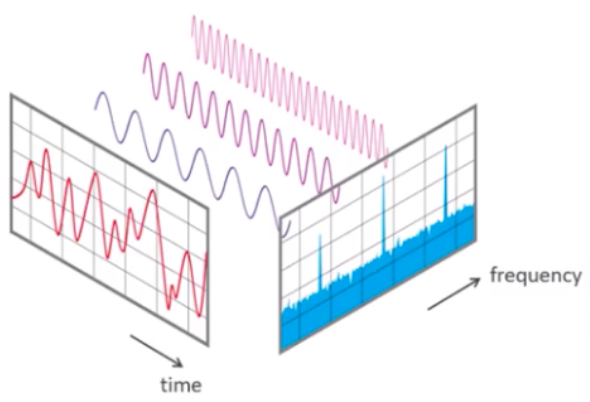
\includegraphics[width=\linewidth]{images/FT.png}
    \caption{Fourier Transform.}
    \label{fig:forecast_prediction}
    \vspace{-10pt}
\end{wrapfigure}
Preprocessing is a crucial step when working with time series data. Unlike regular datasets, time series have a temporal structure that must be preserved and carefully handled. This means that before feeding data into any model, we need to ensure that time information is properly extracted, formatted, and refined.  
High-level preprocessing techniques can be applied depending on the nature of the series:  
\begin{compactitemize}
    \item \textbf{Linear methods} like Fourier Transform or Wavelet Transform, which help in analyzing periodicities and trends.  
    \item \textbf{Non-linear methods:} Hilbert-Huang Transform (HHT).  
\end{compactitemize}

\begin{infobox}[Use Fourier Transformation to Detect Engine Vibrations]
    The \textbf{Fourier Transform} is a powerful tool for analyzing the frequency content of a signal. In practical applications, such as monitoring engine vibrations, it helps identify periodic components that may indicate mechanical issues.  
    
    \begin{compactitemize}
        \item Each mechanical part of an engine tends to vibrate at characteristic frequencies under normal operation.  
        \item By applying the Fourier Transform to vibration data, we can convert the time-domain signal into the frequency domain and identify dominant frequency components.  
        \item \textbf{Abnormal vibrations} often appear as unexpected peaks at frequencies that do not correspond to normal engine operation. For example, a broken bearing or imbalance in a rotor can generate vibrations at specific frequencies.  
        \item Detecting these unusual frequency peaks allows engineers to diagnose potential faults early, before they cause severe damage.  
    \end{compactitemize}
    
    \textbf{Key point:} Fourier analysis is most useful when the problem involves periodic or quasi-periodic signals. In the context of engines, it helps pinpoint which components might be failing based on the frequency patterns of the vibrations.
\end{infobox}
    

\subsection{Data Preparation}
Time series data cannot just be treated like a normal dataset. In the sense, to make predictions we need to have numbers that represent the information, for example the following table
\begin{table}[h!]
    \centering
    \begin{tabular}{|c|c|}
    \hline
    \textbf{Month} & \textbf{Passengers} \\
    \hline
    1949-01 & 112.0 \\
    1949-02 & 118.0 \\
    1949-03 & 132.0 \\
    1949-04 & 129.0 \\
    1949-05 & 121.0 \\
    \hline
    \end{tabular}
\end{table}
represent a time series of monthly airline passengers. if we want make prediction we must transfor data such dates into numerical values. 
\newpage
\subsection{Cyclical Features}
\begin{wrapfigure}{r}{0.2\textwidth}
    \centering
    \vspace{-10pt}
    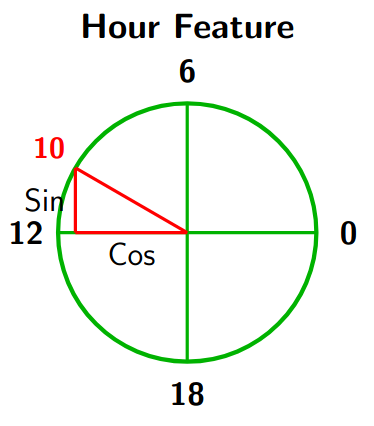
\includegraphics[width=\linewidth]{images/circle.png}
    \label{fig:cyclical_features}
    \vspace{-10pt}
\end{wrapfigure}
Some time-related features are \textbf{cyclical} (e.g., hours of the day, months of the year) and should preserve their periodicity for models to capture patterns correctly:
\begin{compactitemize}
    \item Neural networks work better when inputs have \textbf{zero mean} and \textbf{fixed variance}.  
    \item Cyclical features can be encoded on the \textbf{unit circle} using sine and cosine transformations:
    \[
    \text{Sin(hour)} = \sin\left(\text{hour} \cdot \frac{2\pi}{24}\right), \quad
    \text{Cos(hour)} = \cos\left(\text{hour} \cdot \frac{2\pi}{24}\right)
    \]
    \item The same approach can be applied to months (1--12) or other cyclical variables.
\end{compactitemize}

\section{Recurrent Neural Networks (RNNs)}
Feedforward neural networks (MLPs) compute outputs by propagating information directly from the input $x$ through intermediate hidden layers $h$ to the output $y$. These networks require a fixed-size input because each input neuron corresponds to a specific component of the input vector. In contrast, some network topologies include feedback connections, where outputs are fed back into the network itself. This defines the family of \textbf{Recurrent Neural Networks (RNNs)}, which are specialized for processing sequences. Unlike feedforward networks, RNNs can handle variable-length sequences in the input, in the output, or both, thanks to their internal state that summarizes the sequence seen so far. It is important to note that RNNs are not an architecture per se, but rather a framework that can be implemented in various ways.
\begin{figure}[H]
    \centering
    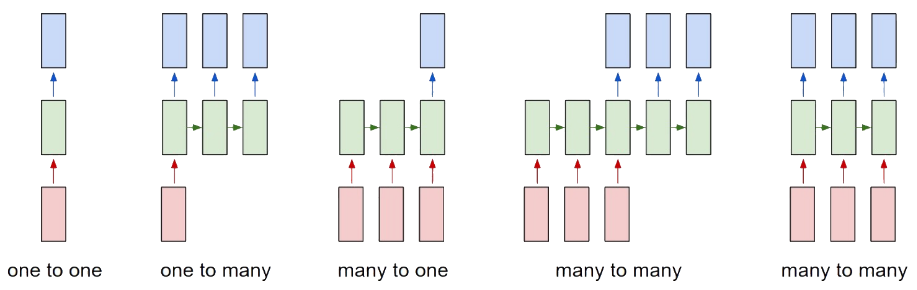
\includegraphics[width=0.85\textwidth]{images/RNN_framwork.png}
    \caption{RNN framework.}
    \label{fig:RNN_framework}
\end{figure}
\begin{infobox}[What is meant by "different size input"]
    Typically, in a \textbf{feedforward neural network (MLP)}, the input must have a \textbf{fixed size}, meaning that the number of input neurons is predetermined and cannot change. Each input neuron corresponds to a specific feature, so if the input vector changes in length, the network cannot process it correctly. Moreover, \textbf{MLPs process the entire input at once} in a single forward pass, without any notion of sequential order.
    
    For example, to predict the next word given a sequence of 5 words, an MLP would require all 5 word embeddings concatenated into a single large input vector. This means the input size grows linearly with the sequence length, making it impractical for long sequences.
    
    In contrast, \textbf{Recurrent Neural Networks (RNNs)} can handle \textbf{sequences of variable length} because they process the input one element at a time and maintain a hidden state that summarizes the information seen so far. In the same prediction task, an RNN would process each word sequentially, updating its hidden state at each step. While each individual element in the sequence must have a fixed dimensionality, the \textbf{number of elements} (i.e., the sequence length) can vary. This allows RNNs to effectively manage sequences of different lengths, as the hidden state carries forward information from earlier timesteps.
\end{infobox}

\subsection{Vanilla RNN}
\begin{wrapfigure}{r}{0.15\textwidth}
    \centering
    \vspace{-10pt}
    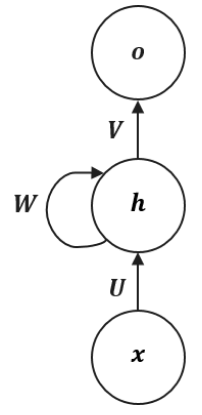
\includegraphics[width=\linewidth]{images/vanilla_RNN.png}
    \label{fig:forecast_prediction}
    \vspace{-10pt}
\end{wrapfigure}
The vanilla RNN is provided with three sets of parameters:
\begin{compactitemize}
    \item $\mathbf{U}$: weights connecting the input $\mathbf{x}_t$ to the hidden state $\mathbf{h}_t$.
    \item $\mathbf{W}$: weights connecting the previous hidden state $\mathbf{h}_{t-1}$ to the current hidden state $\mathbf{h}_t$.
    \item $\mathbf{V}$: weights connecting the hidden state $\mathbf{h}_t$ to the output $\mathbf{o}_t$.
\end{compactitemize}
System dynamics are defined by the following equations:
\[
h^{(t)} = \phi\big(W \, h^{(t-1)} + U \, x^{(t)}\big)
\]
\[
o^{(t)} = V \, h^{(t)}
\]

where $\phi(\cdot)$ is a non-linear activation function, typically $\tanh$ or ReLU. The hidden state $h^{(t)}$ acts as the network's memory, capturing information from previous timesteps. The output $o^{(t)}$ is computed from the current hidden state.

The hidden state $h^{(t)}$ can be intuitively viewed as a \textbf{lossy summary} of the sequence of past inputs fed to the network, in which the main task-relevant aspects of the past sequence of inputs up to time $t$ are stored.  

Since an input sequence of arbitrary length $(x^{(1)}, x^{(2)}, \dots, x^{(t)})$ is mapped into a fixed-size vector $h^{(t)}$, this summary is necessarily \textbf{lossy}.
\begin{infobox}[Important note]
    The parameters $\mathbf{U}$, $\mathbf{W}$, and $\mathbf{V}$ are \textbf{shared across all timesteps}. This weight sharing is crucial because it allows the RNN to generalize across different positions in the sequence. The same transformation is applied at each timestep, enabling the network to learn temporal patterns that are independent of the absolute position in the sequence.
\end{infobox}

\subsection{Training RNNs}
A recurrent computational graph can be unfolded into a sequential computational graph with a respective structure. The output at each timestep is obtained like that:
\[
h^{(t)} = f(h^{(t-1)}, x^{(t)}; \theta)
\]
\begin{figure}[H]
    \centering
    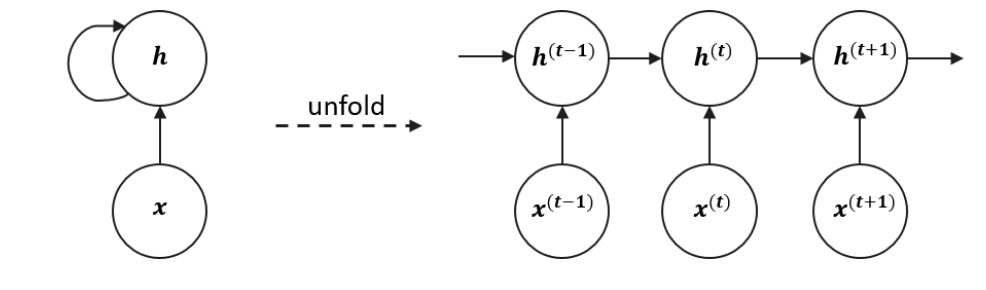
\includegraphics[width=0.65\textwidth]{images/RNN_unfolded.png}
    \caption{RNN unfolded.}
    \label{fig:RNN_unfolded}
\end{figure}
The capacity to unfold a recurrent graph into a DAG (Directed Acyclic Graph) allows for
training a recurrent neural network using standard backpropagation.
Because the gradient conceptually flows backwards through time instead of through layers, this
algorithm is usually referred to as \textbf{backpropagation through time (BPTT)}.

Let's make an example for a simple architecture which processes sequences of length $\tau=3$ and produces an output at the end of the sequence.
\begin{figure}[H]
    \centering
    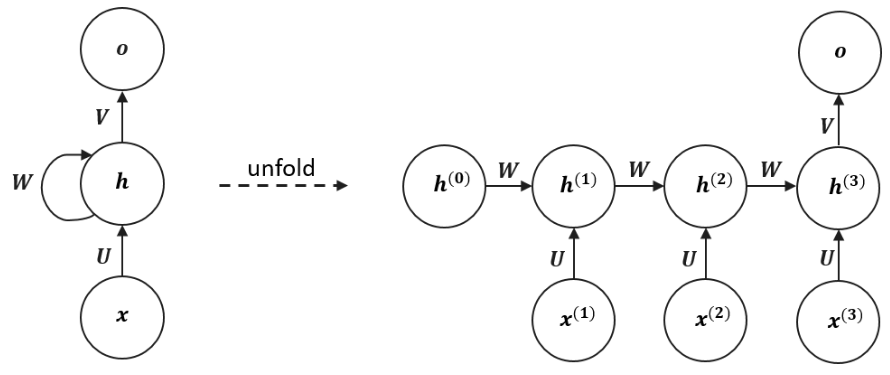
\includegraphics[width=0.65\textwidth]{images/RNN_unfolded_output.png}
    \caption{RNN unfolded with output.}
    \label{fig:RNN_unfolded}
\end{figure}

Now, given a differentiable loss on final output $L(y,o)$,let's compute the derivate of the objective $L$ with respect to the weights $ V, W and U$ and see what happends. The gradients that we must compute is:
\[
\frac{\partial L}{\partial V} = \frac{\partial L}{\partial o} \frac{\partial o}{\partial V}
\]
\[
\frac{\partial L}{\partial W} = \frac{\partial L}{\partial o} \frac{\partial o}{\partial h^{(3)}} 
\sum_{k=0}^{3} \left[ \frac{\partial h^{(3)}}{\partial h^{(k)}} \frac{\partial h^{(k)}}{\partial W} \right]
\]
\[
\frac{\partial L}{\partial U} = \frac{\partial L}{\partial o} \frac{\partial o}{\partial h^{(3)}} 
\sum_{k=0}^{3} \left[ \frac{\partial h^{(3)}}{\partial h^{(k)}} \frac{\partial h^{(k)}}{\partial U} \right]
\]
The first gradient depends only on current state, the other two depend on all previous states.

\textbf{Note:} The calculation of the gradient with respect to $W$ is performed only once, because $W$ is \textbf{shared across all timesteps}!!
\begin{infobox}[Compute the derivatives of $h^{(3)}$ with respect to $h^{(0)}$]
    Consider a simple RNN unrolled over 3 timesteps:
    \[
    h^{(t)} = \phi\big(W h^{(t-1)} + U x^{(t)}\big)
    \]
    with $\phi(\cdot)$ being the ReLU activation function.  
    
    Assume that ReLU is \textbf{always active} (i.e., never zero), so the derivative of $\phi$ is 1 for all units. Then, the derivative of the hidden state at timestep 3 with respect to the initial hidden state $h^{(0)}$ is:
    
    \[
    \frac{\partial h^{(3)}}{\partial h^{(0)}} 
    = \frac{\partial h^{(3)}}{\partial h^{(2)}} \frac{\partial h^{(2)}}{\partial h^{(1)}} \frac{\partial h^{(1)}}{\partial h^{(0)}} = W \cdot W \cdot W = W^3
    \]
    
    \textbf{Implications:}
    
    \begin{compactitemize}
        \item If the values in $W$ are less than 1, raising them to a power (as in $W^3$) makes them even smaller, causing the gradient to shrink as it propagates backward. This is the \textbf{vanishing gradient} problem.
        \item If the values in $W$ are greater than 1, raising them to a power makes them larger, causing the gradient to grow as it propagates backward. This is the \textbf{exploding gradient} problem.
        \item This explains why training vanilla RNNs over long sequences is difficult: the gradient can either vanish or explode, making it hard to learn long-term dependencies.
    \end{compactitemize}
    
    \textbf{Note:} so the part of the update that might be problematic is:
    \[
    \frac{\partial h^{(3)}}{\partial h^{(k)}}
    \]

    \textbf{Note for the exam:} The professor might ask you to compute the derivatives of some functions. So be sure to know how to do it.
\end{infobox}

\subsection{The Challenge of Long-Term Dependencies: Vanishing Gradients}
Looking closer at RNNs, we notice that the gradient at a given timestep depends on gradients at previous timesteps, computed recursively through the chain rule. When using activation functions like \texttt{tanh} or \texttt{sigmoid}, the effect of each timestep on the gradient is naturally limited: for \texttt{tanh} the maximum contribution is 1, and for \texttt{sigmoid} it is even smaller. As a result, when we multiply these contributions across many timesteps, the gradient can shrink rapidly, effectively becoming zero. This phenomenon is known as the \textbf{vanishing gradient problem} and it creates major difficulties in learning long-term dependencies, because the influence of “far-away” timesteps essentially disappears during training.
\subsection{The Challenge of Long-Term Dependencies: Exploding Gradients}
Depending on the network parameters and the choice of activation functions, the opposite problem can occur: the \textbf{exploding gradient problem}. In this case, gradients grow larger and larger as they are propagated backward, eventually causing numerical instability and preventing proper optimization. Both vanishing and exploding gradients can be mitigated through careful weight initialization, the selection of suitable activation functions, and techniques like gradient clipping. While these issues can also appear in deep feedforward networks, they are especially common in recurrent architectures, since an RNN unrolled over time is effectively as deep as the length of the input sequence.
\begin{infobox}[Where do we stop learning?]
    In the vanishing gradient problem, the weights that stop learning are those in the first layers,
    because the gradient becomes smaller and smaller as we go back in time.
    Thus, the weights that are updated the least are those furthest back in time:
    the model gradually forgets older information.

    In the exploding gradient problem, the gradients grow larger and larger as we go back in time.
    As a result, the early weights (those furthest back in time) receive excessively large updates,
    which can dominate the learning process and make the later weights almost irrelevant.
    The model becomes unstable and struggles to learn recent information properly.
\end{infobox}


\section{Advanced Recurrent Architectures}
\textbf{Long Short-Term Memory (LSTM)} and \textbf{Gated Recurrent Unit (GRU)} are more complex recurrent architectures that have been proposed to overcome the issues in the gradient flow and to ease the learning of long-term dependencies thanks to the introduction of \textbf{learnable gating mechanism}.
\begin{figure}[H]
    \centering
    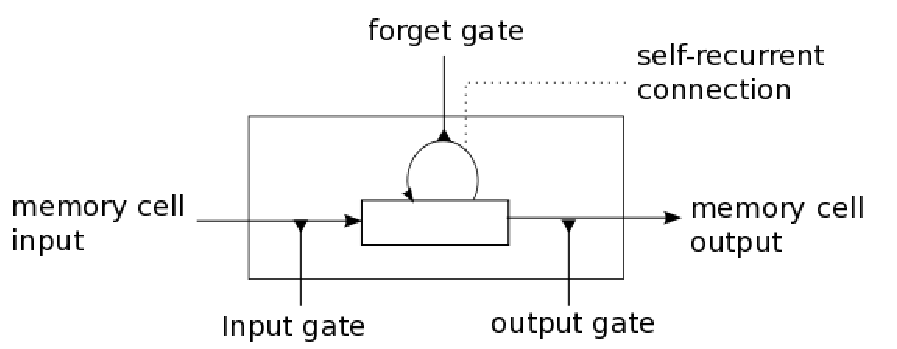
\includegraphics[width=0.6\textwidth]{images/gate.png}
    \caption{Illustration of a learnable gating mechanism used in LSTM and GRU architectures, which controls the flow of information and helps mitigate vanishing and exploding gradient problems.}
    \label{fig:gate}
\end{figure}

\subsection{Long Short-Term Memory networks}
The \textbf{Long Short-Term Memory (LSTM)} network introduces a set of learnable gates that control the flow of information, allowing the network to maintain long-term dependencies more effectively than a vanilla RNN. The main components are the \textbf{input gate} $i$, the \textbf{forget gate} $f$, the \textbf{output gate} $o$, the candidate cell state $\tilde{C}$, the cell state $C^{(t)}$, and the hidden state $h^{(t)}$.  
\begin{figure}[H]
    \centering
    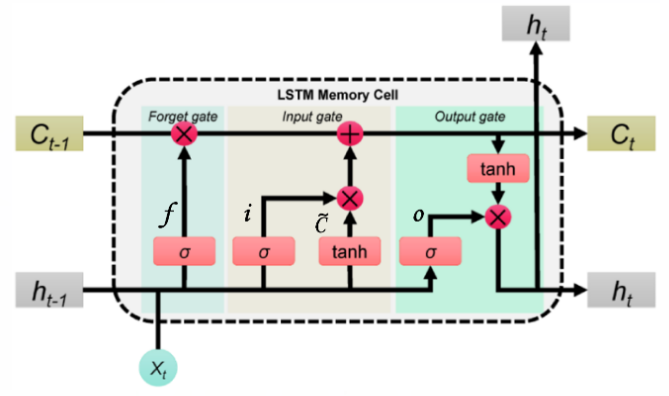
\includegraphics[width=0.65\textwidth]{images/LSTM_model.png}
    \caption{LSTM model.}
    \label{fig:RNN_unfolded}
\end{figure}

The update equations can be compactly written as:
\[
\left\{
\begin{aligned}
i &= \sigma\big(x^{(t)} U_i + h^{(t-1)} W_i\big) \\
f &= \sigma\big(x^{(t)} U_f + h^{(t-1)} W_f\big) \\
o &= \sigma\big(x^{(t)} U_o + h^{(t-1)} W_o\big) \\
\tilde{C} &= \tanh\big(x^{(t)} U_C + h^{(t-1)} W_C\big) \\
C^{(t)} &= C^{(t-1)} \odot f + \tilde{C} \odot i \\
h^{(t)} &= \tanh\big(C^{(t)}\big) \odot o
\end{aligned}
\right.
\]
where $\odot$ denotes element-wise multiplication and $\sigma$ is the sigmoid activation function.  

\textbf{Explanation:}
\begin{compactitemize}
    \item The \textbf{input gate} $i$ controls how much of the candidate cell state $\tilde{C}$ should be added to the cell state.
    \item The \textbf{forget gate} $f$ decides how much of the previous cell state $C^{(t-1)}$ should be retained.
    \item The \textbf{output gate} $o$ regulates how much of the cell state is exposed to the hidden state $h^{(t)}$.
    \item The \textbf{cell state} $C^{(t)}$ acts as the memory of the LSTM, accumulating information over time.
    \item The \textbf{hidden state} $h^{(t)}$ is the output at the current timestep, which also feeds into the next timestep.
\end{compactitemize}
These equations allow LSTMs to selectively remember or forget information at each timestep, addressing the vanishing and exploding gradient problems typical of vanilla RNNs.

\begin{infobox}[The calculus of \texorpdfstring{$\tilde{C}$, $C^{(t)}$ and $h^{(t)}$}{tilde C, C(t) and h(t)}]
    The candidate cell state is computed as:
    \[
    \tilde{C} = \tanh\big(x^{(t)} U_C + h^{(t-1)} W_C\big)
    \]
    The equation is pretty much the same as that we saw in for vanilla RNN architecture. Nonetheless, the amount of influence of $\tilde{C}$ on the LSTM memory cell is controlled by the input gate $i$.

    The update for the update memoruìy cell $C^{(t)}$ is:
    \[
    C^{(t)} = C^{(t-1)} \odot f + \tilde{C} \odot i
    \]
    The forget gate $f$ controls  how much of the memory from previous steps $C^{(t)}$ is retained, while the input gate $i$ supervises the amount of newly computed state $\tilde{C}$ that has to flow into the memory.

    Finally, the hidden state $h^{(t)}$ is computed as:
    \[
    h^{(t)} = \tanh\big(C^{(t)}\big) \odot o
    \]
    The output gate $o$ regulates how much of the cell state $C^{(t)}$ is exposed to the hidden state $h^{(t)}$. The $\tanh$ activation ensures that the values remain bounded between -1 and 1.

    \textbf{Note:} The gate $i$, $f$ and $o$ are \emph{vector} of the same size as the cell state $C$, this insure that multiplication is element-wise. 
\end{infobox}
\newpage
The cell has two inner states:
\begin{compactitemize}
    \item The cell state $C$ represent the \textbf{long-term memory} of the network, and can hold past information without being overwritten quickly.
    \item The hidden state $h$, which also acts as the output, represent the \textbf{short-term memory}; it changes frequently, reflecting the most recent processing, thus containing the information needed for the prediction of the current time step.
\end{compactitemize}




\chapter{TCN and Transformer}

\section{Temporal Convolutional Networks (TCN)}
A sequence model is a model that takes in input a sequence of items (words, letters, time series, audio signals, etc.) and produces an output sequence. Traditional models for sequence modeling include Recurrent Neural Networks (RNNs) and Long Short-Term Memory networks (LSTMs). But recent result indicate that other neural network architectures can outperform this tradutional models.
Typiccaly the name of a single item that give the sequence is a \textbf{token}.

\subsection{Use of Convolutions for Sequence Modeling}
The standard Convolutional Neural Network was first introduced in the LeNet-5 architecture.
Conv2D is generally used on image data. It is called 2-dimensional CNN because the kernel
slides along two spatial dimensions of the input. The principal vantage of using convolutions is that supports spatial relations among pixels.
\begin{figure}[H]
    \centering
    \includegraphics[width=0.3\textwidth]{images/2D_convolution.png}
    \caption{Example of the classic 2D convolution.}
    \label{fig:2D_convolution}
\end{figure}
If we want to use convolutions on sequence data, we can use \textbf{1D convolutions}, which slide the kernel along a single spatial dimension of the input. In this case, the kernel captures temporal relations among tokens in the sequence.
The convolution don't preserve anymore the spatial relations among pixels, but it preserve the temporal dependencies in time series or syntactic order in text. 
\begin{wrapfigure}{r}{0.4\textwidth}
    \centering
    \vspace{-10pt}
    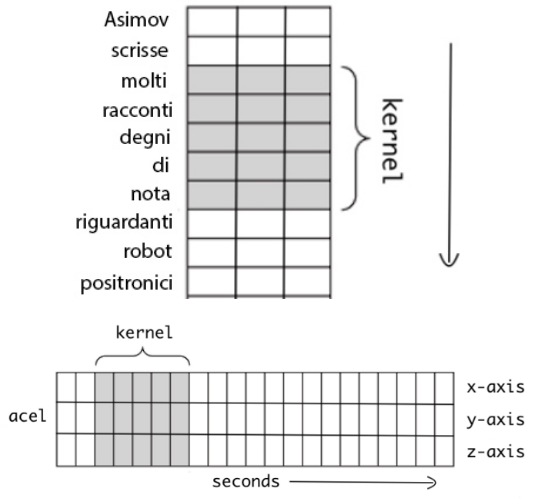
\includegraphics[width=\linewidth]{images/1D_convolution.png}
    \caption{Example of the 1D convolution.}
    \label{fig:1D_convolution}
    \vspace{-10pt}
\end{wrapfigure}
In fact, if we consider text, we can represent each word as a vector of fixed lenght (using word embeddings) and stack these vectors to form a 2D matrix, where each row corresponds to a word in the sequence. Then we can apply 1D convolutions along the temporal dimension (the rows) to capture the relationships between words in the sequence.

The discete 1D convolution is defined as:
\begin{equation}
    (x * w)(n) = \sum_{i=0}^{k-1} x(n-i) w(i)
\end{equation}
Where \textbf{x} is our input vector of lenght \textbf{n}, and \textbf{w} our kernel of lenght \textbf{k}.

\begin{infobox}[Note]
    In the convolution formula we have $x(n - i)$, which implies that the kernel accesses only past values of the input signal. This corresponds to a \textit{causal convolution}, meaning that the output at time $n$ depends only on the current and previous inputs. This property is crucial for sequence modeling tasks, where future information should not be used to predict the next element in the sequence.
\end{infobox}
    
\subsection{Dilated Convolution}
A major disadvantage of using CNNs for sequence modeling is that, in order to achieve a long effective history size (the \textbf{receptive field}), we need an extremely deep network or very large filters. This increases the number of parameters, leading to more complex training, and the network depth can also cause problems such as vanishing or exploding gradients.

\begin{wrapfigure}{r}{0.3\textwidth}
    \centering
    \vspace{-10pt}
    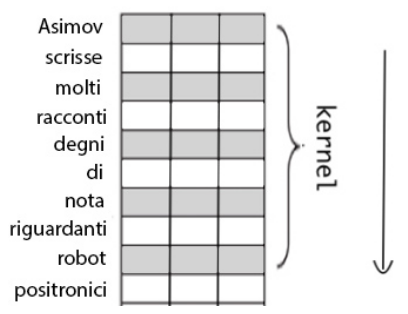
\includegraphics[width=\linewidth]{images/dilatation.png}
    \caption{Example of Dilated Convolution.}
    \label{fig:dilatation}
    \vspace{-10pt}
\end{wrapfigure}

To mitigate this problem we can increase the receptive field using \textbf{dilated convolution}, which introduces gaps between kernel elements to cover a wider input region without increasing the number of parameters.
\begin{equation}
    (x * w)(n) = \sum_{i=0}^{k-1} x(n-d*i) w(i)
\end{equation}
where $d$ is the \textbf{dilation factor}

\newpage
\subsection{Casual Convolution}
\begin{wrapfigure}{r}{0.3\textwidth}
    \centering
    \vspace{-10pt}
    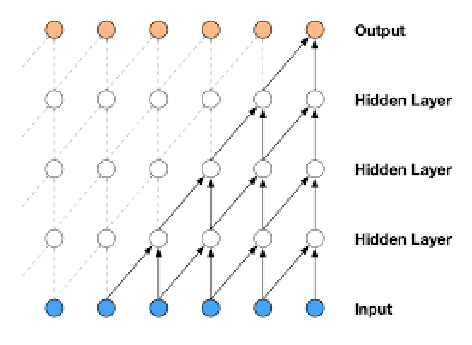
\includegraphics[width=\linewidth]{images/causal_convolution.png}
    \caption{Causal Convolution.}
    \label{fig:causal}
    \vspace{-10pt}
\end{wrapfigure}
A standard convolution can access future input when computing the current output, which may be undesirable for time-series or sequential prediction tasks.

To prevent the model from looking ahead, we can use a \textbf{causal convolution}, which ensures that the output at time step $t$ depends only on inputs from time steps $\leq$ t.

This simple constraint makes CNNs suitable for sequence modeling where causality matters, we will see them again later when discussing autoregressive model.

\subsection{Temporal Convolutional Network}
The \textbf{Temporal Convolutional Network (TCN)} is a model composed of a residual blocks of dilated casual convolution. In TCN each layer use a different \textbf{dilation factor} $d=1,2,4$ and \textbf{filter size} $k=3$
\begin{figure}[H]
    \centering
    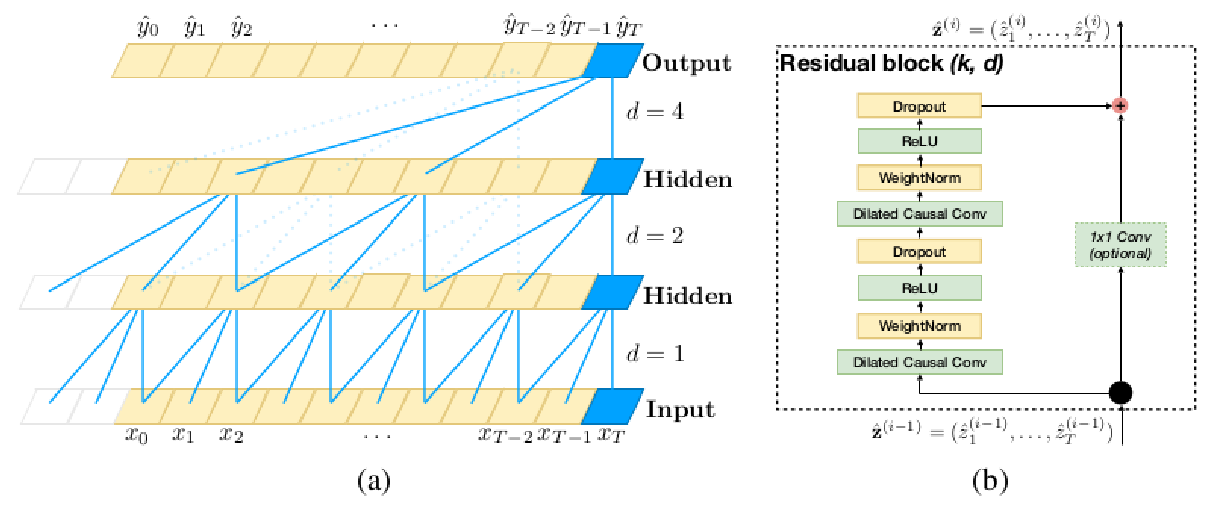
\includegraphics[width=0.9\textwidth]{images/TCN.png}
    \caption{Temporal Convolutional architecture.}
    \label{fig:TCN}
\end{figure}

\begin{infobox}[If the size of the input and output are different?]
    In residual blocks, we need to add the input and the output to form the final output block. To do this, the two elements must have the same size. Therefore, if the input changes its size during the forward pass, we need to apply a convolution to make the input match the size of the output.
\end{infobox}
\begin{infobox}[Effect of the dilated convolution]
    Each element of the output attends to multiple elements of the input, depending on the dilation factor. In this case each element of the outputs attends each element of the input.
\end{infobox}
    
\subsection{TCN vs RNN}
The principal characteristic of TCN compared to RNN are:
\begin{compactitemize}
    \item \textbf{TCN are easier and more stable} to train, they no suffer of vanishing/exploding gradient.
    \item \textbf{Higher effective memory:} longer temporal dependencies can be captured.
    \item \textbf{More parallelizable} and faster on long sequences.
    \item \textbf{Depth=Memory:} receptive field grows with network depth.
    \item Can be equipped by \textbf{explainability modules} 
\end{compactitemize}

\section{Transformer}
Temporal Convolutional Networks (TCNs) are designed to model temporal dependencies in sequential data using a fixed \textit{inductive bias}: local convolutions with an expanding receptive field. This inductive bias is powerful because it enforces causality (outputs depend only on past inputs) and provides stability during training. However, this assumption may not always be appropriate for every problem. In particular, when relevant information is non-local in time or depends on long-range interactions that do not follow a fixed temporal pattern, TCNs may struggle to capture these dependencies. 

For example, in code understanding tasks, the opening of a \texttt{for} loop may influence the value of variables dozens of lines later — a dependency that is difficult to capture using purely local convolutions. This limitation raises the question: can we design a more general architecture that learns how to relate distant elements in a sequence, i.e., how the receptive field should expand, directly from data? The answer is provided by attention-based models, such as Transformers, which can dynamically learn dependencies between distant elements without being constrained by a fixed local receptive field.

\begin{infobox}[What is an inductive bias?]
An \textit{inductive bias} is a set of assumptions that a learning algorithm uses to generalize from training data to unseen data. In the case of TCNs, the inductive bias is that temporal dependencies can be captured using local convolutions with an expanding receptive field. This bias guides the model toward solutions that respect causality and local temporal structure, but it may limit the ability to learn non-local or irregular temporal patterns.
\end{infobox}

\newpage
\subsection{Transformer Architecture}
Transformer network are composed of two main components:
\begin{compactitemize}
    \item \textbf{Encoder}- on the left in the figure.
    \item \textbf{Decoder}- on the right in the figure.
\end{compactitemize}
Each part is built as a stack of $N=6$ layers, forming a deep architecture capable of learning complex dependencies.
\begin{figure}[H]
    \centering
    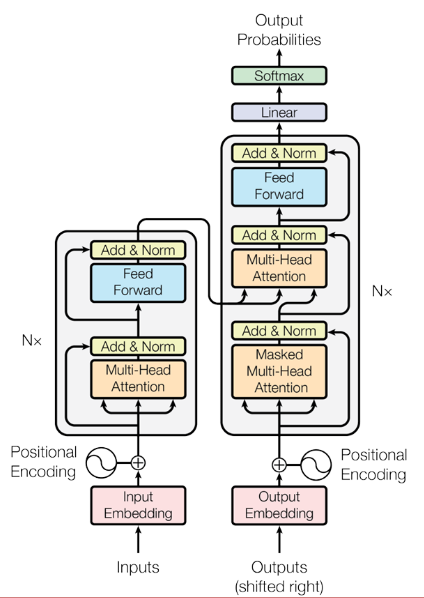
\includegraphics[width=0.5\textwidth]{images/transformer.png}
    \caption{Transformer Architecture.}
    \label{fig:TCN}
\end{figure}
In this course, we will focus on understanding the \textbf{Encoder} part of the Transformer Architecture.

\subsection{Transformer Encoder}
\begin{wrapfigure}{r}{0.2\textwidth}
    \centering
    \vspace{-10pt}
    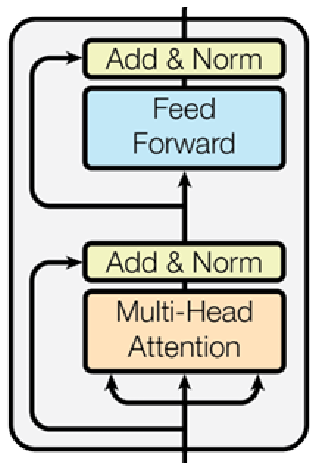
\includegraphics[width=\linewidth]{images/encoder.png}
    \label{fig:encoder}
    \vspace{-10pt}
\end{wrapfigure}
The encoder consists of multiple attention block. The encoder receives an input of embeddings or tokens, each of dimension $d_{model}$, and produces an output of the same shape - with no pooling or dimensionality reduction involved. Usually, we have one token per word or timestep.

Each attention block consist of the following components:
\begin{compactitemize}
    \item A \textbf{Multi-Head Attention (MHA)} layer.
    \item A \textbf{Feed Forward} neural network, composed of two linear layers with a ReLU activation in between.
    \item A \textbf{residual} (or skip) connection after each one of the previus modules, facilitating gradient flow.
    \item \textbf{Layer Normalization} following each residual connection to stabilize training.
\end{compactitemize}

\subsection{Layer Normalization}
Layer Normalization is used to stabilize and speed up training. It normalizes the activations across the features of each example, rather than across the batch as in Batch Normalization. The definition is:
\[
\text{LN}(x) = \frac{x - \mu}{\sigma + \epsilon} \odot \gamma + \beta
\]
where:
\begin{compactitemize}
    \item $\mu=\frac{1}{H}\sum_ix_i$ and $\sigma$ are computed over features.
    \item $\gamma,\beta$ are learnbale affine parameters
    \item normalization is applied \textbf{per token}
\end{compactitemize}
In transformer, LN improves stability in both \textbf{encoder} and \textbf{decoder} stacks.

\begin{infobox}[Difference between LayerNorm and BatchNorm]
    \textbf{Batch Normalization (BatchNorm)} normalizes the activations across the \textit{batch dimension}. For each feature, it computes the mean and variance over the entire mini-batch. This helps to reduce internal covariate shift and can accelerate training, but its behavior depends on the batch size and may be unstable for very small batches.
    
    \textbf{Layer Normalization (LayerNorm)} normalizes the activations across the \textit{feature dimension} for each individual sample. It does not depend on the batch size and is particularly effective in sequence models, such as RNNs and Transformers, where the batch size may vary or be small. LayerNorm ensures consistent normalization for each sample, preserving the temporal or sequential structure.
\end{infobox}

\subsection{The Feed Forward}
The Feed Forward module in Transformers is essentially a classic Multi-Layer Perceptron (MLP). What makes it special is that it is applied \textit{independently to each token} in the sequence. Specifically, for a sequence of token embeddings, the same feed-forward network is applied to each embedding vector without mixing information between different tokens. 

Typically, the feed-forward consists of two linear layers with a non-linear activation function in between (e.g., ReLU). The first layer expands the dimensionality of the token embedding, allowing the network to capture more complex representations, while the second layer projects it back to the original embedding size.

\subsection{The Core Idea of Attention}
In many sequence modeling tasks, not all input elements are equally relevant for producing a given output. Traditional models, such as RNNs or CNNs, process information uniformly, which limits their ability to focus on the most important parts of the input. Attention mechanisms address this limitation by allowing the model to dynamically assign weights to different input elements according to their relevance in the current context. Intuitively, at each step the model asks: ``Which tokens should I pay more attention to right now?''

Formally, for a sequence of input vectors \(X = [x_1, x_2, \dots, x_T]\), the attention mechanism produces a new sequence of contextualized representations \(Z = [z_1, z_2, \dots, z_T]\), where each output vector is a weighted combination of all input vectors:
\[
z_t = \sum_i \alpha_{t,i} \, \mathbf{x}_i, \qquad \alpha_{t,i} = \text{softmax}(s_{t,i})
\]
\begin{infobox}[Important]
The attention coefficients \(\alpha_{t,i}\) are not fixed; they are learned functions of the input, computed through dedicated parametric modules. This allows the model to learn dynamically where to focus depending on the specific input sequence.
\end{infobox}

\subsection{Attention as Content-Based Memory Access}

Instead of compressing all context into a single hidden state (RNNs), the model cna directly \textbf{query the entire sequence of inputs}  to retrieve the most relevant information on demand.

It behaves as a form of \textbf{content-based memory access}: retrieval depends on what is stored, not where it is stored.

The main concepts are:
\begin{compactitemize}
    \item The model mantains a set of \textbf{memory slots}, each represented by a \textbf{key-value} pair.
    \item It generates a \textbf{query} vector describing what it is looking for.
    \item Attention computes the \textbf{similarity} between the query and each key.
    \item Retrieved information is a \textbf{weighted combination of the values}.
\end{compactitemize}

\begin{algorithm}[H]
    \caption{Content-based Retrieval}
    \textbf{Require:}query $q$, keys $\{k_i\}$, values $\{v_i\}$
    \For{each memory slot $i$}{
        $s_i \leftarrow \text{similarity}(q, k_i)$\;
    }
    $\alpha \leftarrow \text{softmax}(s)$ \tcp*[r]{attention weights}
    $z \leftarrow \sum_i \alpha_i v_i$ \tcp*[r]{retrieved information}
    \textbf{return} $z$
\end{algorithm}

\begin{wrapfigure}{r}{0.35\textwidth}
    \centering
    \vspace{-10pt}
    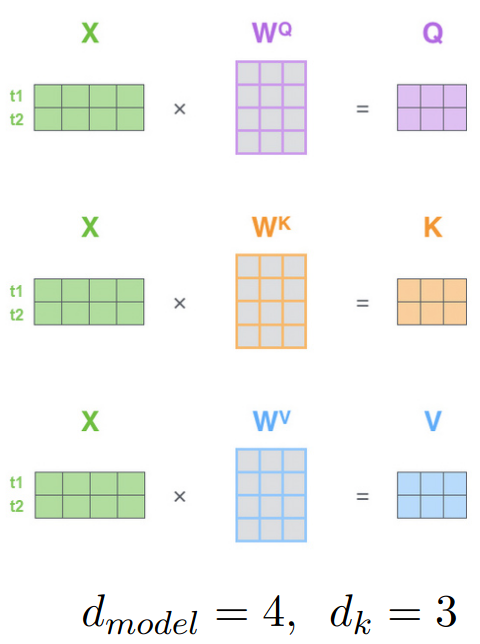
\includegraphics[width=\linewidth]{images/QKV.png}
    \label{fig:QKV}
    \vspace{-10pt}
\end{wrapfigure}

Query, keys, and values are derived from each encoder input vector through linear projections:
\[
Q = X W^Q, \quad K = X W^K, \quad V = X W^V
\]
where \(W^Q, W^K, W^V\) are learnable weight matrices.

These vectors share the dimension \(d_k\), while the input $X$ has dimension \(d_{model}\).

Since all three components originate from the same input ($X$), the attention mechanism is referred to as \textbf{self-attention}.
If the queries, keys, and values come from different sources, it is called \textbf{cross-attention}.

\subsubsection{Single Head Attention}
\begin{wrapfigure}{r}{0.2\textwidth}
    \centering
    \vspace{-10pt}
    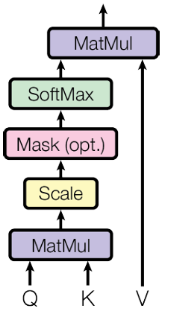
\includegraphics[width=\linewidth]{images/sdpa.png}
    \label{fig:Scaled Dot Product Attention}
    \vspace{-10pt}
\end{wrapfigure}
This mechanism acts as a form of \textbf{content-based memory access}: the model can look back at all inputs and retrieve information on demand.

Formally, the attention operation is defined as:
\[
\text{Attention}(Q, K, V) = \text{softmax}\!\left( \frac{QK^{\top}}{\sqrt{d_k}} \right)V
\]

Here, $Q$, $K$, and $V$ are matrices containing the \textbf{queries}, \textbf{keys}, and \textbf{values}, respectively.  
The dot product $QK^{\top}$ produces a \textbf{similarity matrix} where each entry $(t, i)$ measures how much token $t$ should attend to token $i$.

The dimensionality of $Q$, $K$, and $V$ is $d_k = 64$, which serves as a \textbf{scaling factor} to prevent the dot product from growing too large in magnitude—avoiding saturation of the softmax function that would lead to very small gradients.

\begin{infobox}[Note]
    The softmax is applied row-wise, so that each row of the similarity matrix sums to 1. This ensures that the attention weights for each query form a valid probability distribution over the keys.
\end{infobox}

\subsubsection{Multi-Head Attention}
\begin{wrapfigure}{r}{0.25\textwidth}
    \centering
    \vspace{-10pt}
    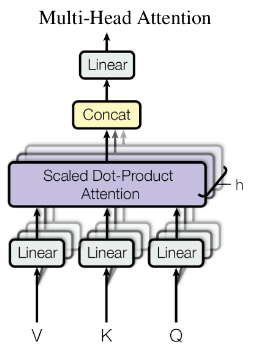
\includegraphics[width=\linewidth]{images/mha.png}
    \label{fig:MHA}
    \vspace{-10pt}
\end{wrapfigure}
The linear projections and the attentions are repeated in parallel multiple times (e.g, h=8), each using a distinct set of weights.

The resulting outputs, each of dimension $d_k$, are then concatenated and passed through a linear layer, which projects the final result to match the dimensionality of $d_{model}$.
Formally, Multi-Head Attention is defined as:
\[
\text{MHA}(Q, K, V) = \text{Concat}(\text{Z}_1, \dots, \text{Z}_h) W^O
\]
where each $Z$ is computed as:
\[
\text{Z}_i = \text{Attention}(X W_i^Q, X W_i^K, X W_i^V)
\]

\begin{figure}[H]
    \centering
    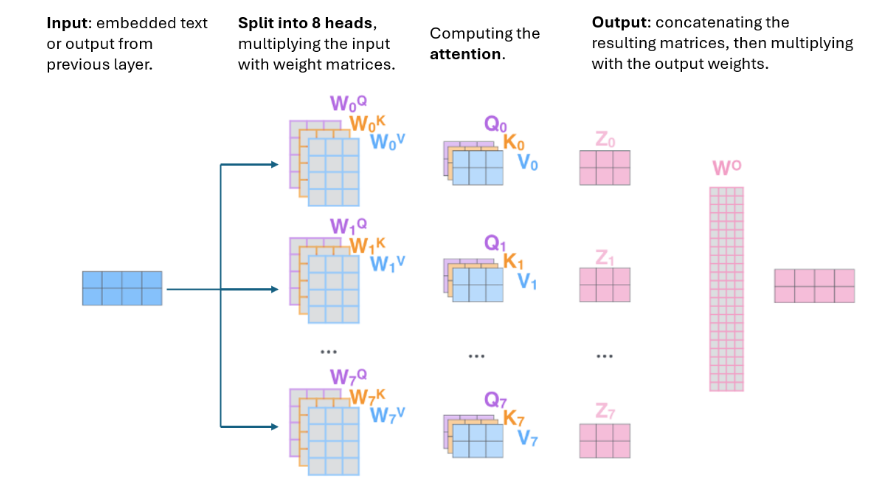
\includegraphics[width=0.9\textwidth]{images/mha2.png}
    \caption{Multi Head Attention.}
    \label{fig:MHA2}
\end{figure}

\begin{infobox}[The problem of concatenate]
    When we use a Multi-Head Attention with $h$ heads, each head produces an output of dimension $d_k$. When we concatenate these outputs, the resulting vector has a dimension of $h \times d_k$. To ensure that the final output of the Multi-Head Attention matches the original input dimension $d_{model}$, we apply a linear transformation using a weight matrix $W^O$ of size $(h \times d_k) \times d_{model}$. This projection step is crucial for maintaining consistency in dimensionality throughout the Transformer architecture.
\end{infobox}

\subsection{From Token Representation to classification}
The encoder outputs a sequence of contextualized token representations, each representing a contextualized version of the corresponding input token. To perform \textbf{classification}, this sequence must be reduced to a single representation. There are two common strategies:
\begin{compactitemize}
    \item \textbf{Average Pooling:} Take the mean of all token embeddings
    \[
    z_{\text{avg}} = \frac{1}{T} \sum_{t=1}^{T} \mathbf{z}_t
    \]
    and feed it to a MLP classifier.
    \item \textbf{[CLS] Token:} Introduce a special classification token prepended to the input sequence. Its final embedding $z_{[CLS]}$ is used as the global representation and passed therough an MLP for classification.
\end{compactitemize}

\subsection{Summary: From TCN to Transformers}

Both TCNs and Transformers are powerful architectures for modeling sequential data, but they rely on different inductive biases and mechanisms.

\begin{compactitemize}
    \item \textbf{Temporal Convolutional Networks (TCN):}
    \begin{compactitemize}
        \item Model temporal dependencies via \textbf{causal and dilated convolutions}.
        \item Capture \textbf{local-to-mid-range temporal structure} efficiently.
        \item \textbf{Stable and easy to train}.
    \end{compactitemize}
    
    \item \textbf{Transformers:}
    \begin{compactitemize}
        \item Model dependencies through \textbf{attention}.
        \item No fixed receptive field — can learn \textbf{arbitrary long-range relations}.
        \item Naturally handle \textbf{multimodal and non-sequential contexts}.
        \item Foundation of modern architectures (\textbf{BERT, GPT, ViT, etc.}).
    \end{compactitemize}
\end{compactitemize}

\textbf{Takeaway:} TCNs impose a \textbf{structured inductive bias}; Transformers learn to \textbf{discover structure directly from data}.

\section{Loss Functions for Regression}
When training models for regression tasks, the choice of loss function is crucial as it directly influences the model's learning process and performance. Here are some commonly used loss functions for regression:
\begin{compactitemize}
    \item The \textbf{Mean Squared Error (MSE)} loss is defined as:
    \[
    \   text{MSE} = \frac{1}{N} \sum_{i=1}^{N} (y_i - \hat{y}_i)^2
    \]
    This loss penalizes large errors more strongly due to the squaring of the differences, making it sensitive to outliers. It is also smooth and differentiable, which is beneficial for optimization.
    \item The \textbf{Mean Absolute Error (MAE)} loss is defined as:
    \[
    \text{MAE} = \frac{1}{N} \sum_{i=1}^{N} |y_i - \hat{y}_i|
    \]
    This loss treats all errors equally, making it more robust to outliers compared to MSE. However, it is less sensitive to small errors and can be less smooth, which may affect optimization.
\end{compactitemize}

\subsection{From Regression to Classification via Binning}
In most cases, predicting continuous values directly can be challenging. An alternative approach is instead of predicting continuos values directly (regression), we can discretize the target into intervals (called \textbf{bins}) and train a model to classify which interval the target belong to.

Let's see an example of age prediction from an image:
\begin{compactitemize}
    \item \textbf{Target variable:} age $\in [0, 100]$
    \item \textbf{Discretization:} Define $K$ bins, e.g.:
    \[
    [0-10], [10-20], [20-30], \dots, [90-100]
    \]
    \item \textbf{Training:} Train a classifier with $K$ output classes (one per age interval).
    \item \textbf{Prediction:} The final age prediction can be:
    \begin{compactitemize}
        \item The \textbf{center of the predicted bin}, e.g., $25$ for $[20-30]$, or
        \item A \textbf{weighted average of bin centers} using class probabilities.
    \end{compactitemize}
\end{compactitemize}

Let's see why converting a regression task into a classification problem can be useful:
\begin{compactitemize}
    \item By discretizing the target variable into bins, we can train a \textbf{classifier} using standard \textbf{cross-entropy loss}.
    \item This approach naturally allows us to \textbf{capture uncertainty} through the predicted probability distribution across bins, giving more informative predictions than a single point estimate.
\end{compactitemize}

\subsection{Limitations of MSE and MAE}
Both MAE and MSE assume \textbf{symmetric errors}: overestimating and underestimating the target by the same amount incur equal penalties. However, in many real-world applications, the cost of overestimation and underestimation may differ significantly. For example:
\begin{compactitemize}
    \item In financial forecasting, overestimating revenue may lead to overspending, while underestimating may result in missed opportunities.
    \item In medical diagnosis, overestimating the severity of a condition may lead to unnecessary treatments, while underestimating may delay critical care.
\end{compactitemize}
We may want to estimate not a single "average" value, but a range of possible outcomes, this motivates the use of \textbf{Quantile Loss}.

\subsection{Understanding Quantiles}
\begin{wrapfigure}{r}{0.35\textwidth}
    \centering
    \vspace{-10pt}
    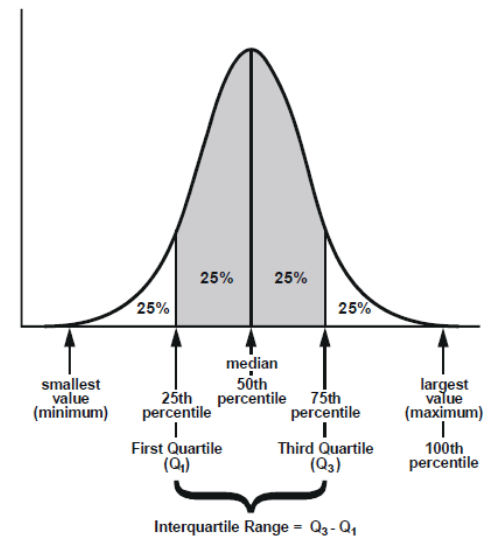
\includegraphics[width=\linewidth]{images/dis.png}
    \label{fig:MHA}
    \vspace{-10pt}
\end{wrapfigure}
The $\tau$-quantile of a distribution is the value $q_{\tau}$ such that $P(Y \le q_{\tau}) = \tau$.
Let's see some examples:
\begin{compactitemize}
    \item The $0.5$-quantile (median) is the value that splits the distribution in half: $50\%$ of values are below it, and $50\%$ are above it.
    \item The $0.25$-quantile (first quartile) is the value below which $25\%$ of the data fall.
    \item The $0.75$-quantile (third quartile) is the value below which $75\%$ of the data fall.
    \item The $0.1$-quantile is the value below which $10\%$ of the data fall.
\end{compactitemize}

\begin{infobox}[Note]
    In gaussian distribution, mena, median and mode are all the same value, but in general this is not true.
\end{infobox}

\subsection{Quantile Loss Function}
The goal of quantile regression is to estimate the $\tau$-quantile of the target variable given the input features. The quantile loss function, is defined as:
\[
L_{\tau}(y, \hat{y}) = \begin{cases}
\tau (y - \hat{y}) & \text{if } y > \hat{y} \\
(1 - \tau) (\hat{y} - y) & \text{if } y \leq \hat{y}
\end{cases}
\]
where: 
\begin{compactitemize}
    \item $y$ is the true target value and the $\hat{y}$ is the etimate
    \item $\tau \in (0, 1)$ is a \textbf{hyperparameter} that controls which quantile we want to estimate.
\end{compactitemize}

Let's see some questions:
\begin{compactitemize}
    \item What happens when $\tau = 0.5$?  
    The Quantile Loss collapses to the \textbf{Mean Absolute Error (MAE)}.
    
    \item How are errors weighted when $\tau = 0.9$?  
    Underestimations ($\hat{y} < y$) are penalized $9\times$ more than overestimations, so it’s more convenient for the model to slightly overpredict.
    
    \item When $\tau = 0.9$, is the model encouraged to underestimate or overestimate the target?  
    It tends to \textbf{overestimate}, aligning predictions with the 90th percentile.
\end{compactitemize}

In summary, the main properties of Quantile Loss are:
\begin{compactitemize}
    \item \textbf{Asymmetric}: underestimations and overestimations are penalized differently.
    \item Encourages the model to predict the \textbf{$\tau$-quantile} of the $Y$.
\end{compactitemize}
The intuition is that the model "pays" more for errors on one side of the prediction, depending on the chosen quantile $\tau$.
\chapter{Graph Neural Networks}

\section{Little back to Convolutional Neural Networks}
\begin{wrapfigure}{r}{0.4\textwidth}
    \centering
    \vspace{-10pt}
    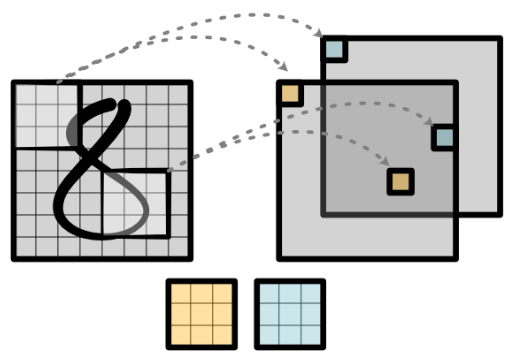
\includegraphics[width=\linewidth]{images/ex_conv.png}
    \label{fig:conv}
    \vspace{-10pt}
\end{wrapfigure}
The \textbf{2D spatial cross-correlation} between an input image $I$ and a square kernel $K \in R^{d \times d}$ is defined as:
\[
S(i, j) = \sum_{m=-k}^{k} \sum_{n=-k}^{k} I(i + m, j + n) \cdot K(m, n)
\]
where:
\begin{compactitemize}
    \item $d = 2k + 1$: kernel size (square)
    \item $I(i+m, j+n)$: pixel value at position $(i+m, j+n)$ in the input image
    \item $K(m, n)$: kernel weight
\end{compactitemize}

\subsection{1D Cross-Correlation on a 1D Euclidean Lattice} 
\begin{wrapfigure}{r}{0.5\textwidth}
    \centering
    \vspace{-10pt}
    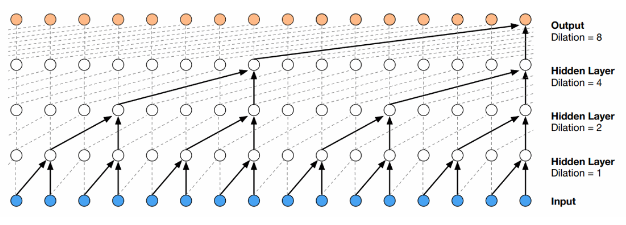
\includegraphics[width=\linewidth]{images/1D.png}
    \label{fig:conv1D}
    \vspace{-10pt}
\end{wrapfigure}
Just like in 2D, the 1D grid can be seen as a discretization of a continuous Euclidean line $\mathbb{R}$, sampled at regular intervals.  
In this case both input and kernel are defined on a 1D Euclidean space, and the kernel slides along this lattice, computing local interactions at each position.  
This setup is widely used in domains such as audio processing, NLP, and time series analysis.

\subsection{2D Cross-Correlation on a 2D Euclidean Lattice} 
The image can also be represented as a 2D grid graph, where each pixel is a node connected to its neighboring pixels. In particular:
\begin{compactitemize}
    \item Each pixel lies on a \textbf{discrete 2D lattice} $\mathbb{Z}^2$ embedded in Euclidean plane.
    \item Cross-correlation slides a small kernel across this grid, visiting each location systematically.
    \item At each location, the kernel interacts with a local patch, treating it as a \textbf{neighborhood in 2D space}.
\end{compactitemize}

\begin{figure}[H]
    \centering
    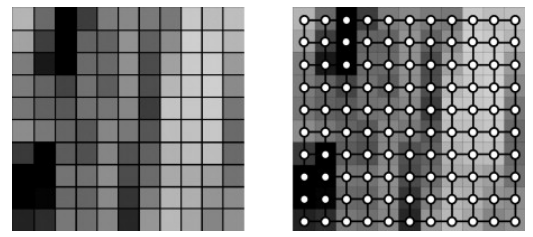
\includegraphics[width=0.5\textwidth]{images/image_graph.png}
    \caption{Image represented as a graph.}
    \label{fig:image_graph}
\end{figure}

\begin{infobox}[Note]
    Although the operation is discrete, the grid itself can be viewed as a sampling of a continuous 2D Euclidean space.
\end{infobox}

\subsection{A Graph Viewpoint}
Under this new viewpoint, the input image can be interpreted as a \textbf{signal lying on a (Euclidean) graph}.  
A graph $G = (V, E)$ consists of a set of nodes (vertices) $V$ and a set of edges $E \subseteq V \times V$.  
Graphs can be:
\begin{compactitemize}
    \item \textbf{Directed or undirected}
    \item \textbf{Weighted or unweighted}
\end{compactitemize}

A \textbf{lattice graph} is a particular case where nodes are arranged on a regular grid (e.g., 1D, 2D, or 3D).  
In the case of a 2D Euclidean lattice:
\begin{compactitemize}
    \item Each pixel corresponds to a node in the graph.
    \item Each node is associated with a feature vector (e.g., a triplet of raw RGB values).
    \item The edge set $E$ connects each node to its spatial neighbors using a fixed connectivity rule (e.g., 4-connected: top, bottom, left, right).
\end{compactitemize}

\subsection{Problem of Standard N-D Convolution}
A limitation of traditional convolutional architectures is that they assume data is defined over \textbf{regular Euclidean grids} (e.g., 1D signals, 2D images).  
These models rely on:
\begin{compactitemize}
    \item \textbf{Fixed neighborhood structures}, determined by the lattice topology.
    \item \textbf{Shift-invariance} properties, which hold only in regular domains.
\end{compactitemize}

However, many real-world data domains — such as social networks, molecular structures, and transportation systems — are inherently \textbf{non-Euclidean}.  
This motivates the need for generalizing convolutional operations to arbitrary graph structures, leading to the development of \textbf{Graph Neural Networks (GNNs)}.

\begin{figure}[H]
    \centering
    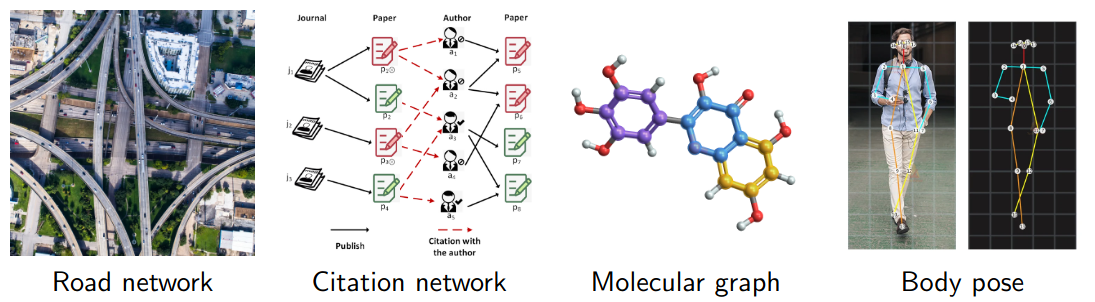
\includegraphics[width=0.9\textwidth]{images/non_euclidian_domains.png}
    \caption{Example of no Euclidian Domains.}
    \label{fig:image_graph}
\end{figure}

\section{Graph Neural Networks}
The objective of Graph Neural Networks (GNNs) is to define a NN that can handle \textbf{graph-structured data}. In particular a NN that can handle:
\begin{compactitemize}
    \item \textbf{Irregular structures}: node may have different number of neighbors (no fixed-size receptive field).
    \item \textbf{No spatial locality}: unlike images, there is no inherent notion of distance or order between nodes.
    \item \textbf{Permutation invariance}: the model's output should not depend on the order in which nodes are processed.  So if we have two identical graphs, but with different node ordering, the output should be the same.
    \WFclear
    \item \textbf{No global coordinate system}: we cannot rely on a fixed layout or orientation.
    \item \textbf{Dynamic topology}: edge connectivity may evolve or depend on node features.
\end{compactitemize}
\begin{figure}[H]
    \centering
    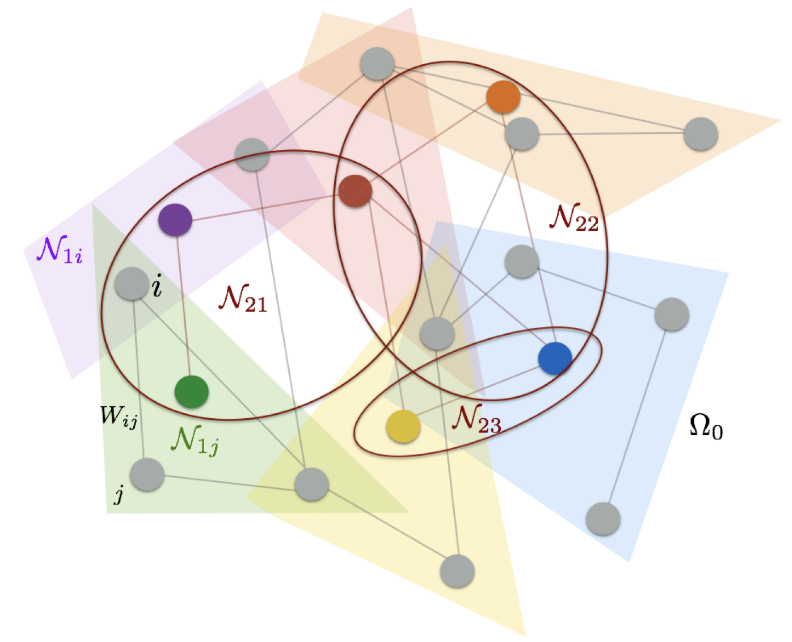
\includegraphics[width=0.3\textwidth]{images/graph_data.png}
    \caption{Graph data structured.}
    \label{fig:image_graph}
\end{figure}

\textbf{Graph Convolutional Networks} introduced by Kipf and Welling generalize convolution to graph-structured data convolution to graph-structured data. As with standard neural network like MLPs and CNNs:
\begin{compactitemize}
    \item A GNNs is structured in multiple succesive layers.
    \item We have input features, hidden activations (often call \textbf{node embeddings}), activation functins and output responses.
    \item Gradient descent and backpropagation are used to train the model.
\end{compactitemize}


A key idea of GCNs is to define a \textbf{message-passing}, where each node updates its feature representation by aggregating information from its neighbors. The processes follow these steps:
\begin{wrapfigure}{r}{0.5\textwidth}
    \centering
    \vspace{-10pt}
    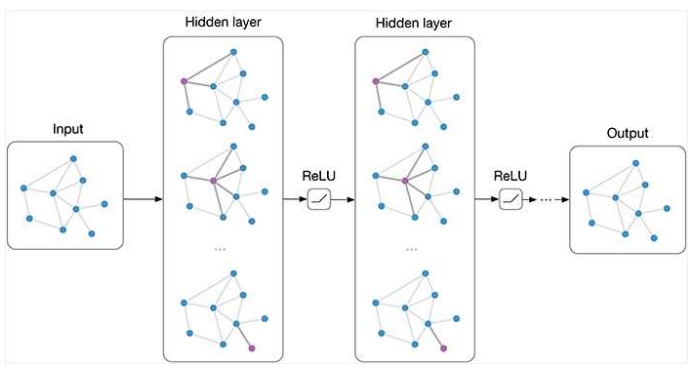
\includegraphics[width=\linewidth]{images/GNN.png}
    \label{fig:conv1D}
    \vspace{-10pt}
\end{wrapfigure}
\begin{compactitemize}
    \item \textbf{Step 1}: Leveraging the graph structure, each node collects information from its neighbors by combining their embeddings. The embeddings are combined through an aggregation (poolin) function (e.g., sum, mean, max).
    \item \textbf{Step 2}: The aggregated information is then passed through a neural network layer (e.g, a simple MLP) to generate a new representation (embedding) for the node. This results in an  \textbf{updated node representation} that captures both its own features and those of its local neighborhood.
\end{compactitemize}

\begin{infobox}[How Graph Convolutional Layer Works]
    \textbf{Input for each node $v$:}
\begin{compactitemize}
    \item Node's own feature vector: $\mathbf{h}_v^{(l)}$ (embedding at layer $l$)
    \item Neighbor feature vectors: $\{\mathbf{h}_u^{(l)} : u \in \mathcal{N}(v)\}$ where $\mathcal{N}(v)$ is the set of neighbors
\end{compactitemize}

\textbf{Computation steps:}
\begin{enumerate}
    \item \textbf{Aggregation}: Combine neighbor features
    $$\mathbf{m}_v^{(l)} = \text{AGGREGATE}\left(\{\mathbf{h}_u^{(l)} : u \in \mathcal{N}(v)\}\right)$$
    Common aggregation functions:
    \begin{compactitemize}
        \item Sum: $\mathbf{m}_v = \sum_{u \in \mathcal{N}(v)} \mathbf{h}_u^{(l)}$
        \item Mean: $\mathbf{m}_v = \frac{1}{|\mathcal{N}(v)|} \sum_{u \in \mathcal{N}(v)} \mathbf{h}_u^{(l)}$
        \item Max: $\mathbf{m}_v = \max_{u \in \mathcal{N}(v)} \mathbf{h}_u^{(l)}$
    \end{compactitemize}
    
    \item \textbf{Update}: Combine aggregated message with node's own features
    $$\mathbf{h}_v^{(l+1)} = \sigma\left(\mathbf{W}^{(l)} \cdot \text{CONCAT}(\mathbf{h}_v^{(l)}, \mathbf{m}_v^{(l)}) + \mathbf{b}^{(l)}\right)$$
    where $\mathbf{W}^{(l)}$ is a learnable weight matrix, $\mathbf{b}^{(l)}$ is a bias, and $\sigma$ is an activation function (e.g., ReLU).
\end{enumerate}

\textbf{Output}: Updated node embedding $\mathbf{h}_v^{(l+1)}$ that incorporates information from the local neighborhood.
\end{infobox}

\subsection{An example of Graph Convolutional Layer}
\begin{wrapfigure}{r}{0.3\textwidth}
    \centering
    \vspace{-10pt}
    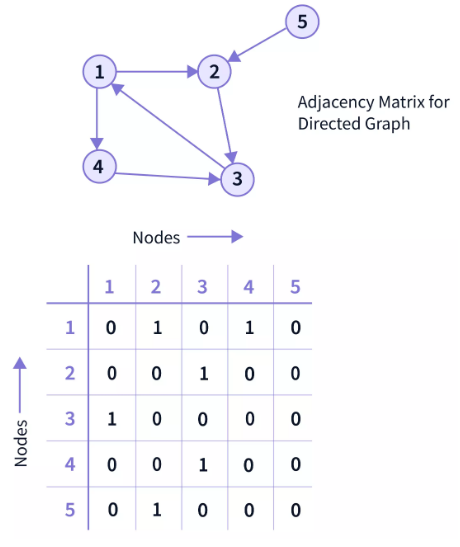
\includegraphics[width=\linewidth]{images/GCN_example.png}
    \label{fig:conv1D}
    \vspace{-10pt}
\end{wrapfigure}
GCN Layer (Kipf and Welling, 2017) represents one of the most prominent examples of graph-based neural netowrks. The net has two input:
\begin{compactitemize}
    \item \textbf{Node features matrix} $X \in R^{nxd}$: each row corresponds to the feature vector of a node.
    \item \textbf{Adjacency matrix} $A \in R^{nxn}$: encodes the graph structure, where $A_{ij} = 1$ if there is an edge from node $i$ to node $j$, and $0$ otherwise. This if the matrix is binary, but it can also be weighted.
\end{compactitemize}

\subsection{The Role of the Adjacency Matrix}
The \textbf{adjacency matrix} $\mathbf{A}$ is a fundamental component of Graph Neural Networks, serving multiple critical roles in the learning process. First, it acts as a \textbf{structural prior} that encodes the geometry and topology of the underlying domain. By explicitly representing which nodes are connected, the adjacency matrix provides the model with essential information about the spatial or relational structure of the data, allowing the GNN to respect and leverage these constraints during feature propagation. This is particularly important because, unlike grid-structured data (e.g., images), graphs lack inherent spatial regularity, and the adjacency matrix compensates for this by defining the neighborhood structure explicitly.

Beyond encoding structure, the adjacency matrix plays a crucial role in \textbf{regularization and generalization}. By limiting message passing to only those connections defined in $\mathbf{A}$, the model enforces locality, meaning that information flow is restricted to meaningful, structurally-relevant paths rather than allowing unconstrained communication between all nodes. This locality constraint acts as a powerful form of inductive bias that helps prevent overfitting: the model cannot learn arbitrary dependencies between distant or unrelated nodes, but must instead focus on learning patterns that respect the graph's topology. This injection of domain-specific structure into the model architecture enables better generalization to unseen graphs with similar structural properties, as the learned features are inherently tied to the relational structure rather than being purely data-driven.

The adjacency matrix can be obtained or constructed through various approaches, depending on the application:

\begin{compactitemize}
\item \textbf{Domain knowledge}: The graph structure is defined manually based on expert knowledge of the problem domain. Examples include human skeleton graphs where edges connect anatomically-linked joints, molecular graphs where edges represent chemical bonds between atoms, or citation networks where edges indicate references between papers.

\item \textbf{Heuristic construction}: When the graph structure is not explicitly given, it can be constructed using data-driven heuristics. Common approaches include:
\begin{compactitemize}
\item \textit{k-nearest neighbors (k-NN)}: Connect each node to its $k$ closest neighbors in feature space, typically using Euclidean distance or cosine similarity.
\item \textit{Distance thresholds}: Create edges between nodes whose feature vectors are within a specified distance threshold $\epsilon$.
\item \textit{Similarity-based}: Define edge weights based on feature similarity, creating a weighted adjacency matrix where $A_{ij} = \text{sim}(\mathbf{x}_i, \mathbf{x}_j)$.
\end{compactitemize}
\end{compactitemize}

\subsection{Message Passing}
The core operation of Graph Convolutional Networks (GCNs) is defined by a \textbf{layer-wise propagation rule} that updates node embeddings by aggregating information from their neighborhoods. The mathematical formulation of this process is given by:

$$\mathbf{H}^{(l)} = \sigma\left(\hat{\mathbf{D}}^{-\frac{1}{2}} \hat{\mathbf{A}} \hat{\mathbf{D}}^{-\frac{1}{2}} \mathbf{H}^{(l-1)} \mathbf{W}^{(l)}\right)$$

where the key components are:

\begin{compactitemize}
\item $\hat{\mathbf{A}} = \mathbf{A} + \mathbf{I}$: the adjacency matrix with added self-loops. The addition of the identity matrix $\mathbf{I}$ ensures that each node also considers its own features during aggregation, not just those of its neighbors.

\item $\hat{\mathbf{D}}$: the degree matrix of $\hat{\mathbf{A}}$, defined as a diagonal matrix where $\hat{D}_{i,i} = \sum_j \hat{A}_{i,j}$. This matrix captures how many connections (including the self-loop) each node has.

\item $\hat{\mathbf{D}}^{-\frac{1}{2}} \hat{\mathbf{A}} \hat{\mathbf{D}}^{-\frac{1}{2}}$: the symmetric normalization of the adjacency matrix. This normalization is crucial because it prevents nodes with many neighbors from having disproportionately large feature values, ensuring numerical stability and balanced information flow.

\item $\mathbf{H}^{(l-1)} \in \mathbb{R}^{|V| \times F_{l-1}}$: the matrix of node embeddings from the previous layer, where $|V|$ is the number of nodes and $F_{l-1}$ is the feature dimension at layer $l-1$.

\item $\mathbf{W}^{(l)} \in \mathbb{R}^{F_{l-1} \times F_l}$: a learnable projection matrix that transforms features from dimension $F_{l-1}$ to $F_l$. This is the trainable component of the layer.

\item $\sigma(\cdot)$: a non-linear activation function (e.g., ReLU) that introduces non-linearity into the model.
\end{compactitemize}

\textbf{Alternative per-node formulation:} For binary adjacency matrices, the GCN operation can be expressed at the individual node level, which provides clearer intuition about the message-passing mechanism:

\begin{enumerate}
\item \textbf{Aggregation}: Each node $v$ collects and normalizes features from its neighbors (including itself):
$$\mathbf{a}_v^{(l)} = \sum_{u \in \mathcal{N}(v) \cup \{v\}} \frac{1}{\sqrt{\hat{d}_v \hat{d}_u}} \mathbf{h}_u^{(l-1)}$$
where $\hat{d}_v$ and $\hat{d}_u$ are the degrees of nodes $v$ and $u$ in $\hat{\mathbf{A}}$. The normalization factor $\frac{1}{\sqrt{\hat{d}_v \hat{d}_u}}$ ensures that nodes with many neighbors don't dominate the aggregation.

\item \textbf{Projection}: The aggregated features are linearly transformed:
$$\mathbf{z}_v^{(l)} = \mathbf{a}_v^{(l)} \cdot \mathbf{W}^{(l)}$$

\item \textbf{Non-linearity}: An activation function is applied to produce the final updated embedding:
$$\mathbf{h}_v^{(l)} = \sigma(\mathbf{z}_v^{(l)})$$
\end{enumerate}

This formulation makes explicit that each node's embedding is updated using features from $\mathcal{N}(v)$ (the set of its immediate neighbors $u$, each with its degree $\hat{d}_u$) and from itself, with appropriate normalization based on the connectivity structure.

\subsubsection{Receptive Field and Theoretical Motivations}
A single GCN layer performs aggregation over the \textbf{first-order neighborhood}, meaning it only considers nodes that are directly connected (1-hop neighbors). However, by stacking multiple GCN layers, the model can capture information from increasingly distant parts of the graph. Specifically, an $L$-layer GCN has a receptive field of $L$ hops: after $L$ layers, each node's representation incorporates information from all nodes within $L$ steps in the graph. For example, a 2-layer GCN for node classification can be written as:

$$\mathbf{Z} = \text{softmax}\left(\hat{\mathbf{D}}^{-\frac{1}{2}} \hat{\mathbf{A}} \hat{\mathbf{D}}^{-\frac{1}{2}} \sigma\left(\hat{\mathbf{D}}^{-\frac{1}{2}} \hat{\mathbf{A}} \hat{\mathbf{D}}^{-\frac{1}{2}} \mathbf{X} \mathbf{W}^{(0)}\right) \mathbf{W}^{(1)}\right)$$

where $\mathbf{X}$ is the input feature matrix, and the final softmax produces class probabilities for node classification tasks.

The GCN architecture is not just an empirical design but has solid theoretical foundations rooted in spectral graph theory. Specifically, the GCN can be understood as a first-order approximation of spectral graph convolutions, which are based on the spectral formulation of convolution operations on graphs. This connection to spectral theory provides mathematical justification for why the normalized adjacency matrix and the specific aggregation scheme lead to effective learning on graph-structured data.

\section{Applications of Graph Neural Networks}

\subsection{Node Classification}
The task is predict a label for each node in the graph, in details:
\begin{compactitemize}
    \item Each node $v \in V$ has an input feature vector $\mathbf{x}_v$.
    \item Through multiple layers, the GNN encodes it into a node embedding $h_v \in R^d$.
    \item A classification layer maps the embedding to class scores:
    \[
        z_v = W h_v + b \in R^C
    \]
    \item The predicted label is then:
    \[
        \hat{y}_v = \text{argmax}_c z_{v}[c]
    \]
\end{compactitemize}
The output is $Z \in R^{NxC}$

The are two main settings:
\begin{compactitemize}
    \item \textbf{Transductive Setting}: The entire graph is available during training, but labels are known only for a subset of nodes. The goal is to predict label for the remaining nodes in the same graph. The model can be leverage connections to all nodes (labeled and enlabeled). Unlabeled nodes influence learning through shared structure, even if not supervised directly.
    \item \textbf{Inductive Setting}: The model must generalize to \textbf{unseen nodes or graphs.} These nodes are not part of the training graph. Predictions rely only on node features and local structure. The model learns representations that transfer across graphs.
\end{compactitemize}

\begin{figure}[H]
    \centering
    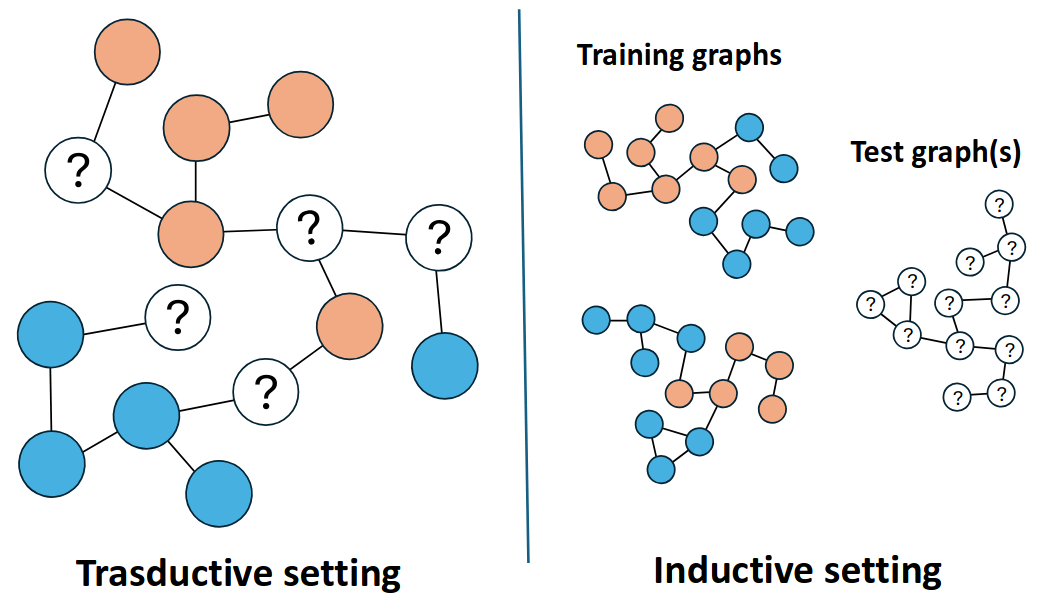
\includegraphics[width=0.6\textwidth]{images/node_classification.png}
    \caption{Node classification settings.}
    \label{fig:image_graph}
\end{figure}

\subsection{Link Prediction}
The task is to predict the existence of edges between pairs of nodes. In details:
\begin{compactitemize}
    \item Given two nodes $u$ and $v$, the goal is to predict if $(u, v) \in E$
    \item This is a binary classification task on node pairs (or multi-class for edge types).
    \item Common pipeline:
    \begin{compactitemize}
        \item Learn node embeddings $h_u$ and $h_v$ via GNN.
        \item Compute edge representation:
        \[
            s_{uv}=Decoder(h_u, h_v)
        \]
        \item Map to class scores:
        \[
            z_{uv} = W s_{uv} + b \in R^C
        \]
        \item Predict edge existence:
        \[
            \hat{y}_{uv} = \text{argmax}_c z_{uv}[c]
        \]
    \end{compactitemize}
\end{compactitemize}

Applications include:
\begin{compactitemize}
    \item Social network link prediction (friend recommendations)
    \item Biological networks: Predict protein-protein or drug-target interactions.
    \item Recommender systems (user-item interactions)
\end{compactitemize}

\subsection{Graph Classification}
The task is to predict a label for an entire graph. In details:
\begin{compactitemize}
    \item Each graph $G_i = (V,E)$ is treated as a single data point.
    \item Node features are processed by GNN layers to obtain node embeddings $h_v$.
    \item A textbf{global pooling} functions aggregates them into a single graph-level vector:
    \[
        h_{graph} = \text{POOLING}(\{h_v | v \in V\})
    \]
\end{compactitemize}
A finale MLP predicts the graph label:
\[
    \hat{y}_{G}=MLP(h_{graph})
\]
The pooling function can be:
\begin{compactitemize}
    \item \textbf{Global Average Pooling}: $h_{graph} = \frac{1}{|V|} \sum_{v \in V} h_v$
    \item \textbf{Attention-based Pooling}: $h_{graph} = \sum_{v \in V} \alpha_v h_v$  with $\alpha_v = softmax(a^T h_v)$
\end{compactitemize}
While these two approaches summurize the entire set of vertices in a single step, other methods allow for hierarchical pooling, similar to what is done in standard CNNS.

\begin{figure}[H]
    \centering
    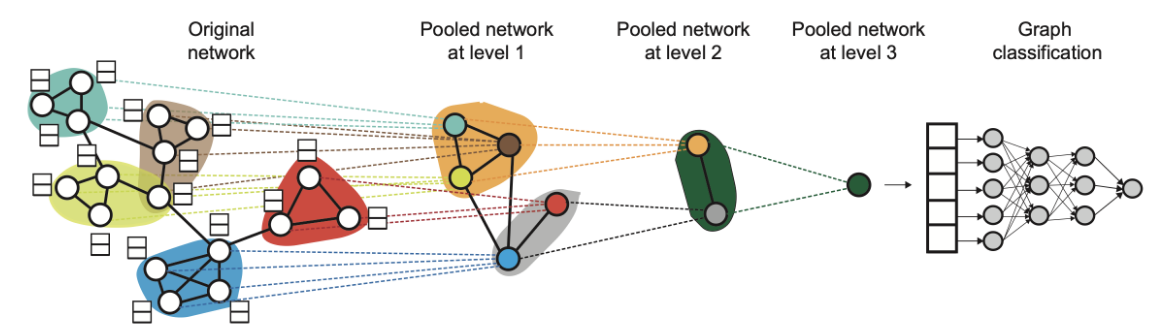
\includegraphics[width=0.9\textwidth]{images/hierarchical_pooling.png}
    \caption{Example of hierarchical pooling.}
    \label{fig:image_graph}
\end{figure}

\begin{wrapfigure}{r}{0.3\textwidth}
    \centering
    \vspace{-10pt}
    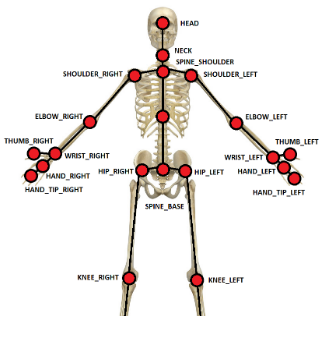
\includegraphics[width=\linewidth]{images/scheletro.png}
    \label{fig:conv1D}
    \vspace{-10pt}
\end{wrapfigure}
A classic application of graph classification is \textbf{Action Recognition}. Given a sequence of human poses represented as skeleton graphs, the goal is to classify the action being performed (e.g., walking, running, jumping). 
Graphs are constructed with:
\begin{compactitemize}
    \item \textbf{Spatial edges}: connections between joints.
    \item \textbf{Temporal edges}: same joint across frames.
\end{compactitemize}
The GNNs or Spatio-Temporal GCNs (ST-GCNs) are used to.


\begin{figure}[H]
    \centering
    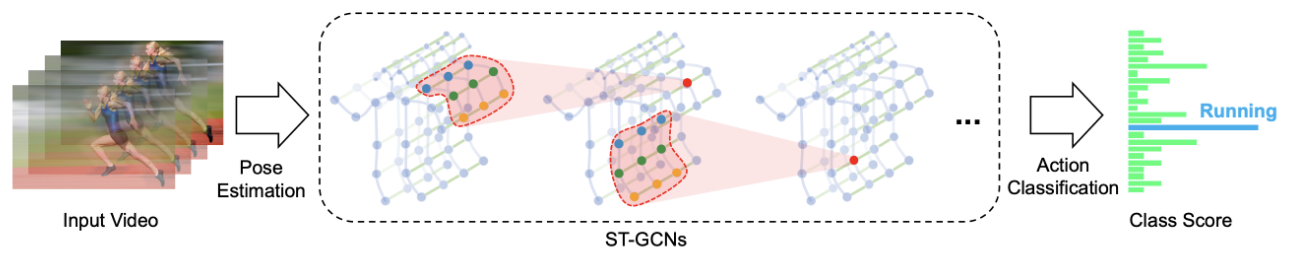
\includegraphics[width=0.9\textwidth]{images/Action.png}
    \caption{Example of action recognition.}
    \label{fig:image_graph}
\end{figure}


\section{Graph Attention Networks (GATs)}

\subsection{Limitations of GCNs}

While Graph Convolutional Networks provide a powerful framework for learning on graph-structured data, they suffer from several fundamental limitations that restrict their expressiveness and practical applicability. Recall the layer-wise propagation rule of GCN:

$$\mathbf{H}^{(l)} = \sigma\left(\hat{\mathbf{D}}^{-\frac{1}{2}} \hat{\mathbf{A}} \hat{\mathbf{D}}^{-\frac{1}{2}} \mathbf{H}^{(l-1)} \mathbf{W}^{(l)}\right)$$

The main problems with this formulation are:

\begin{compactitemize}
\item \textbf{Over-smoothing}: As the number of layers increases, node representations tend to become increasingly similar and eventually indistinguishable. This happens because repeated neighborhood averaging causes all nodes to converge toward similar feature distributions, losing the discriminative power needed for downstream tasks. This severely limits the depth of GCN architectures.

\item \textbf{Uniform aggregation}: All neighbors contribute equally (or only degree-normalized) to a node's representation, without any adaptive weighting or attention mechanism. The model cannot distinguish between important and less important neighbors—every connection in the graph is treated with the same significance, regardless of the actual relevance of the information being passed.

\item \textbf{Limited expressivity}: GCNs are heavily dependent on the structure encoded in the input adjacency matrix $\mathbf{A}$. The model cannot adapt or learn which connections are truly important for the task at hand; it is constrained by the pre-defined graph topology. If the adjacency matrix does not accurately reflect the relationships relevant to the learning task, the GCN's performance will be fundamentally limited.
\end{compactitemize}

These limitations motivate the development of more flexible architectures that can learn adaptive, task-specific edge weights rather than relying solely on the fixed graph structure.

\subsection{Graph Attention Networks: Core Idea}
Graph Attention Networks (GATs), introduced by Veličković et al., address the limitations of GCNs by incorporating an \textbf{attention mechanism} that allows the model to learn which neighbors are most relevant for each node. The key innovations of GATs are:
\begin{compactitemize}
\item \textbf{Learned edge weights}: The model learns adaptive attention coefficients that determine how much each neighbor contributes to a node's updated representation. This eliminates the need for pre-defined weighted adjacency matrices, as the importance of each connection is learned from data.
\item \textbf{Local adaptivity}: Different neighbors of the same node can receive different attention weights, allowing the model to focus on the most informative connections. This enables more flexible and expressive aggregation compared to the uniform (or degree-normalized) weighting in GCNs.
\item \textbf{Structural awareness}: Through the attention mechanism, each node selectively attends to its neighboring nodes as defined by the input adjacency matrix. However, unlike GCNs, the strength of these connections is not fixed but rather learned during training, making the model more robust to noise or irrelevant edges in the graph structure.
\end{compactitemize}
The attention mechanism allows GATs to automatically identify which neighbors carry the most relevant information for updating each node's features, leading to more discriminative representations and better performance on graph learning tasks.

\subsection{GAT Architecture: Detailed Mechanism}

The GAT layer computes updated node representations through a sequence of operations that combine linear transformations with learned attention weights. The process can be broken down into the following steps:

\begin{compactitemize}
\item \textbf{Step 1: Linear Projection.} First, a shared linear transformation is applied to all node features to project them into a new feature space:
$$\mathbf{h}_i^W = \mathbf{W}\mathbf{h}_i \quad \text{for each node } i$$
where $\mathbf{W} \in \mathbb{R}^{F' \times F}$ is a learnable weight matrix that projects features from dimension $F$ to dimension $F'$. This transformation is shared across all nodes, similar to the projection in GCNs, and allows the model to learn task-relevant feature representations.

\item \textbf{Step 2: Attention Score Computation.} Next, the model computes an unnormalized attention score (or affinity score) between node $i$ and each of its neighbors $j$:
$$e_{ij} = \text{LeakyReLU}\left(\mathbf{a}^\top [\mathbf{h}_i^W \| \mathbf{h}_j^W]\right)$$
where $[\cdot \| \cdot]$ denotes vector concatenation, $\mathbf{a} \in \mathbb{R}^{2F'}$ is a learnable weight vector that parameterizes the attention mechanism, and LeakyReLU is the activation function applied to introduce non-linearity. The concatenation $[\mathbf{h}_i^W \| \mathbf{h}_j^W]$ creates a $2F'$-dimensional vector that captures both the features of the central node $i$ and its neighbor $j$. The learned vector $\mathbf{a}$ then computes a scalar attention score that indicates how important neighbor $j$'s features are to node $i$. Importantly, this attention score is \textbf{asymmetric}: the importance of $j$ to $i$ (captured by $e_{ij}$) may differ from the importance of $i$ to $j$ (captured by $e_{ji}$), allowing the model to capture directed relationships even in undirected graphs.

\item \textbf{Masked Attention.} In its most general formulation, the attention mechanism could allow every node to attend to every other node in the graph, which would discard all structural information encoded in the adjacency matrix. To preserve the graph structure, GATs employ \textbf{masked attention}: the attention score $e_{ij}$ is computed only for nodes $j \in \mathcal{N}(i)$, where $\mathcal{N}(i)$ denotes the first-order neighbors of node $i$ (including $i$ itself, if self-loops are used). This way, the graph topology acts as a mask that restricts attention to structurally connected nodes, while still allowing the model to learn the relative importance of these connections. An important advantage of masked attention is that \textbf{the graph need not be undirected}: if an edge $j \to i$ is not present in the adjacency matrix, the computation of $\alpha_{ij}$ is simply omitted. This makes GATs naturally applicable to directed graphs without requiring symmetrization.

\item \textbf{Step 3: Attention Normalization.} The unnormalized attention scores are then normalized across all neighbors of node $i$ using a softmax function:
$$\alpha_{ij} = \frac{\exp(e_{ij})}{\sum_{k \in \mathcal{N}(i)} \exp(e_{ik})}$$
This normalization ensures that the attention coefficients $\alpha_{ij}$ sum to 1 across all neighbors, making them interpretable as the relative importance of each neighbor. The softmax operation also ensures numerical stability and makes the attention coefficients differentiable, allowing end-to-end training via backpropagation.

\item \textbf{Step 4: Weighted Aggregation.} Finally, the updated node representation is computed as a weighted sum of the transformed neighbor features, where the weights are the learned attention coefficients:
$$\mathbf{h}_i' = \sigma\left(\sum_{j \in \mathcal{N}(i)} \alpha_{ij} \mathbf{h}_j^W\right)$$
where $\sigma$ is a non-linear activation function (e.g., ReLU or ELU). This aggregation is fundamentally different from GCNs: instead of using fixed (or degree-normalized) weights, each neighbor's contribution is modulated by the learned attention coefficient $\alpha_{ij}$, allowing the model to emphasize important neighbors and downweight less relevant ones.

\item \textbf{Step 5: Multi-Head Attention (optional).} To stabilize the learning process and increase the model's expressive power, GATs employ \textbf{multi-head attention}, similar to the mechanism used in Transformers. The idea is to execute $K$ independent attention mechanisms in parallel, each with its own learnable parameters $\mathbf{W}^{(k)}$ and $\mathbf{a}^{(k)}$. The outputs from all $K$ attention heads are then combined. For intermediate layers, the outputs are typically concatenated:
$$\mathbf{h}_i' = \|_{k=1}^K \sigma\left(\sum_{j \in \mathcal{N}(i)} \alpha_{ij}^{(k)} \mathbf{W}^{(k)} \mathbf{h}_j\right)$$
where $\|$ denotes concatenation and $\alpha_{ij}^{(k)}$ are the attention coefficients computed by the $k$-th attention head. Note that with $K$ heads, each producing $F'$-dimensional features, the final output $\mathbf{h}_i'$ will have dimension $KF'$ rather than $F'$. For the final layer (e.g., in classification tasks), averaging is typically used instead of concatenation:
$$\mathbf{h}_i' = \sigma\left(\frac{1}{K} \sum_{k=1}^K \sum_{j \in \mathcal{N}(i)} \alpha_{ij}^{(k)} \mathbf{W}^{(k)} \mathbf{h}_j\right)$$
Multi-head attention provides several benefits: it allows the model to attend to different aspects of the neighborhood simultaneously, reduces the risk of overfitting to specific attention patterns, and empirically leads to more stable training and better generalization.
\end{compactitemize}

\textbf{Additional enhancements:} Like many modern deep learning architectures, GATs can be combined with \textbf{residual connections} to facilitate gradient flow and enable training of deeper networks, further improving their expressiveness and mitigating over-smoothing issues.

\begin{table}[h]
    \centering
    \caption{Comparison between GAT and Self-Attention (Transformers)}
    \begin{tabular}{|p{3.5cm}|p{5.5cm}|p{5.5cm}|}
    \hline
    \textbf{Aspect} & \textbf{GAT} & \textbf{Self-Attention (Transformers)} \\
    \hline
    Input structure & Graph (nodes + edges) & Sequence (e.g., tokens) \\
    \hline
    Neighborhood & Defined by adjacency matrix & Full attention (every token attends to all others) \\
    \hline
    Sparsity & Sparse: only local neighbors & Dense: full pairwise interactions \\
    \hline
    Attention mechanism & Single-layer MLP over concatenated node pairs & Dot-product between learned query and key vectors \\
    \hline
    Position encoding & Implicit via graph topology & Explicit (e.g., sinusoidal or learned) \\
    \hline
    Inductive bias & Local, relational inductive bias from graph edges & Temporal or spatial bias via positional encodings \\
    \hline
    \end{tabular}
    \label{tab:gat_vs_transformer}
\end{table}

\subsection{GATv2: Addressing Static Attention Limitations}

While GATs represent a significant advancement over standard GCNs by introducing attention mechanisms, subsequent analysis revealed fundamental limitations in their expressiveness. The authors of GATv2 identified that the standard GAT formulation does not truly compute \textbf{dynamic attention}. Instead, the attention mechanism in GAT is essentially \textbf{static}: for any given query node, the scoring of its neighbors is monotonic with respect to per-node scores computed independently of the query. This means that the relative ranking of neighbors remains the same regardless of which node is performing the attention computation, severely limiting the model's ability to capture context-dependent relationships. As a concrete consequence, GAT cannot even express simple alignment problems where the importance of a neighbor should vary based on the features of the central node.

\textbf{GATv2 solution.} To address this limitation, the authors proposed GATv2, which achieves truly dynamic attention by simply \textbf{modifying the order of operations} in the attention score computation. Specifically, instead of computing:
$$e_{ij} = \text{LeakyReLU}\left(\mathbf{a}^\top [\mathbf{h}_i^W \| \mathbf{h}_j^W]\right)$$

GATv2 applies the non-linearity before the final projection:
$$e_{ij} = \mathbf{a}^\top \text{LeakyReLU}\left(\mathbf{W}[\mathbf{h}_i \| \mathbf{h}_j]\right)$$

This seemingly minor change has profound theoretical implications: GATv2 becomes a \textbf{universal approximator} for attention functions, meaning it can theoretically express any attention pattern. As a result, GATv2 is strictly more expressive and powerful than the original GAT, while maintaining the same computational complexity and implementation simplicity.

\section{GraphCast: Weather Forecasting with GNNs}

GraphCast, developed by DeepMind in 2023, is a state-of-the-art model for medium-range weather prediction that applies Graph Neural Networks to atmospheric forecasting. The model represents the Earth's atmosphere as a graph where:

\begin{compactitemize}
\item \textbf{Nodes}: grid points on a spherical mesh (icosahedral grid)
\item \textbf{Edges}: connect spatially adjacent locations
\item \textbf{Node features}: meteorological variables (wind, temperature, pressure, etc.)
\end{compactitemize}

\textbf{Results.} For 10-day forecasts, GraphCast is competitive with traditional physics-based models like HRES—the top deterministic operational system in the world—while achieving much faster inference.

\textbf{Architecture.} GraphCast uses temporal sequence modeling to forecast future atmospheric states. The model employs message-passing GNN layers and is trained on decades of weather data. A key design feature is the use of multiple graph meshes at different resolutions: coarse meshes capture global context and large-scale patterns, while fine meshes capture local weather phenomena. Each resolution corresponds to a distinct icosahedral mesh that provides nearly uniform coverage of the Earth's surface.

\begin{figure}[H]
    \centering
    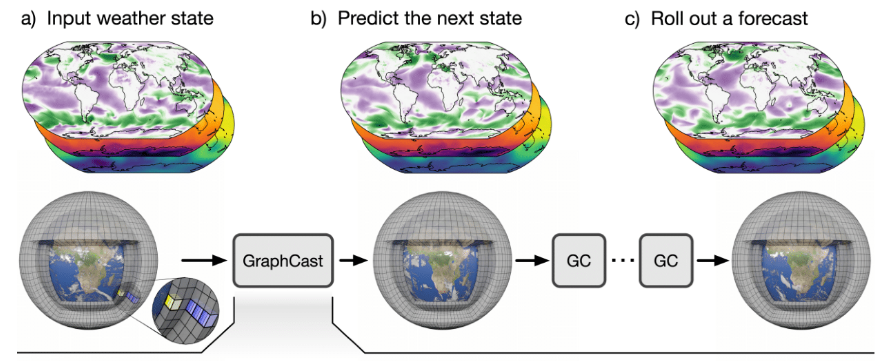
\includegraphics[width=0.9\textwidth]{images/GC1.png}
    \label{fig:image_graph}
\end{figure}
\begin{figure}[H]
    \centering
    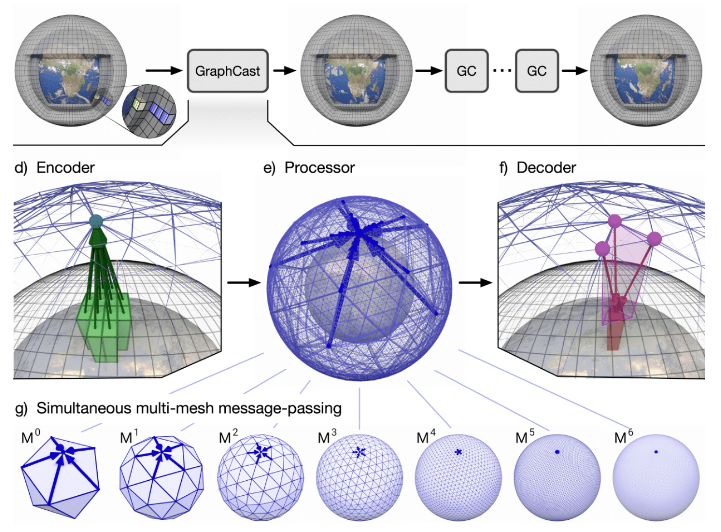
\includegraphics[width=0.9\textwidth]{images/GC2.png}
    \caption{Graph-Cast.}
    \label{fig:image_graph}
\end{figure}

\chapter{Autoencoders}

\section{Unservised Learning}
Mosto impressive results in deep learning have been obtained with \textbf{purely supervised learning} methods. In vision typically classification (e.g. object recognition).
Although progress has been slower, unsupervised learning is likely to remain important for future advances in deep learning. 

\begin{figure}[H]
    \centering
    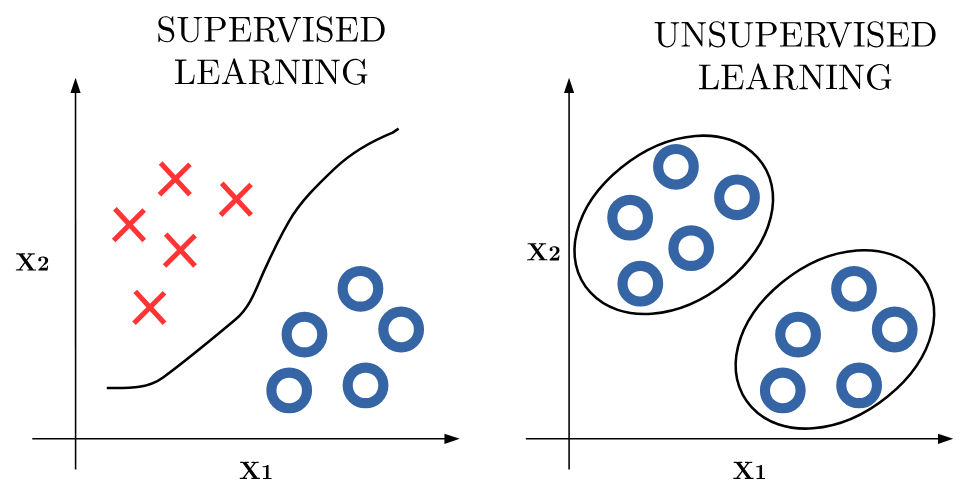
\includegraphics[width=0.5\textwidth]{images/supervised_unsupervised.png}
    \caption{Difference between supervised and unsupervised learning.}
    \label{fig:MHA2}
\end{figure}

\subsection{Why Unsupervised Learning?}
Deeper models lead to \textbf{more parameters}, which implies the requirement for \textbf{high number of training data} to avoid overfitting. The reason are:
\begin{enumerate}
    \item It is often easier to obtain unlabelled data then labeled data, which can require human annotation. We can also exploit unlabelled data, it is much more readibly and often free.
    \item Unsupervised learning involves observing several examples of a random vector $x$ and attempting to implicity or explicity learn the probability distribution $p(x)$, or some interesting properties of that distributions. We can capture enough information about the observed variables to ask new questions about them.
    \item Another two characteristic of unsupervised learning are:
        \begin{compactitemize}
            \item \textbf{Optimization}: unsupervised pre-training helps in initializing the parameters at a good position in the optimization landscape, significantly better than any position given by random inizialization.
            \item \textbf{Regularization}: unsupervised learning is a good regularizer for supervised learning, it helps in reducing overfitting. 
        \end{compactitemize}
\end{enumerate}
This advantage is evident in pratical applications, such as transfer learning and domain adaptation.
\begin{figure}[H]
    \centering
    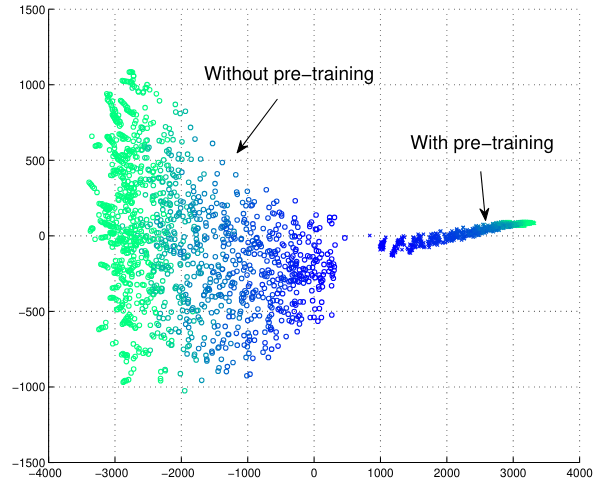
\includegraphics[width=0.35\textwidth]{images/SP.png}
    \caption{SOMAP embedding of functions represented by 50 networks w and w/o pre-training (Erhan et al., 2010).}
    \label{fig:MHA2}
\end{figure}

\section{Learning Rapresentations}
Take the \textbf{MNIST} dataset as an example, the image were centred in a $28x28$ image. Suppose each pixel is representable with a binary value: what is the cardinality of the whole set consisting of all the $28x28$ binary image?
\begin{equation}
    D^{i}_{2,784}=2^{28x28} = 2^{784}=1.01745...10^{236}
\end{equation}
The problem is that most of ${2}^{784}$, or more in general of $R^N$, consists of \textbf{invalid inputs}. 

Similary, if you generate a document by picking letters uniformly ar random, what is the probability that you will get a meaningful English-language text? \textbf{Almost zero}, because the distribution of natural leanguage sequences occupies a very little volume in total space of sequences of letters.
\newpage
\subsection{Manifold Assumption}
Many machine learning problems seem hopeless if we except the machine learning algorithm to learn functions with interesting variations across all of $R^N$.
\begin{wrapfigure}{r}{0.4\textwidth}
    \centering
    \vspace{-10pt}
    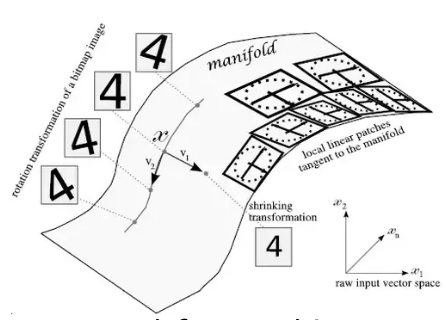
\includegraphics[width=\linewidth]{images/manifold.png}
    \label{fig:Scaled Dot Product Attention}
    \vspace{-10pt}
\end{wrapfigure}
\textbf{Manifold Assumption}: data lies approximately on a manifold of much lower dimension than the input space, where the actual degrees of freedom that can account for the variability in the data is \textbf{much lesser}.

When the data lies on a low-dimensional \textbf{manifold}, it can be most natural for machine learning algorithms to \textbf{REPRESENT} the data in terms of coordinates in the manifold than in terms of coordinates in $R^N$ .
\vspace{0.5cm}

To find a good representation of the data, it's better understand what we mean by \textbf{good representation}, so:
\begin{compactitemize}
    \item We are looking for a representation that \textbf{preserves as much information} about $x$ as possible while obeying some penalty or constraint.
    \item This additional constraint keep the learned representation \textbf{simple} or \textbf{more accessible} than $x$ itself.
    \item The new representation can be \textbf{task-specific} or \textbf{task-agnostic}.
\end{compactitemize}

\begin{infobox}[Difference between Task-specific and Task-agnostic]
    A \textbf{task-specific representation} is a representation of the data that is learned with the goal of performing well on a particular task, such as classification or segmentation. It keeps only the information that is directly useful for that task and may discard details that are irrelevant for it. Because of this, task-specific representations are usually very effective for the task they are designed for, but they do not generalize well to different tasks.

    A \textbf{task-agnostic representation}, instead, is learned without focusing on a particular task. Its goal is to capture general and meaningful structure in the data that can be reused for many different tasks. These representations are more flexible and transferable, but may be less optimal when applied to any single specific task compared to task-specific ones.
\end{infobox}

Beyond thus consideration, there are some \textbf{criteria} that a good representation should satisfy:
\begin{compactitemize}
    \item \textbf{Lower dimensional representation}: attempt to \textbf{compress} as much information as possible about $x$ in a smaller representation.
    \item \textbf{Sparse representation}: embed the dataset into a representation whose entries are \textbf{mostly zero} for most inputs.
    \item \textbf{Indipendent representation}: attempt to \textbf{disentangle} the factors of variatiom underlying the data distribution such that dimension of the representation are statistically independent.
\end{compactitemize}

\begin{infobox}[Sparse Representation Example]
    Consider an input image representing a handwritten digit. Instead of activating many features at once, a sparse representation will activate only a few neurons corresponding to specific local patterns (for example: one neuron for a vertical stroke, one for a curve, etc.). 
    
    \textbf{Example:}
    
    \[
    x = \text{image of "7"}
    \]
    Sparse code:
    \[
    z = [0, 0, 1.2, 0, 0, 0.8, 0, 0, 0, 0]
    \]
    
    Only the features for \textit{"vertical line"} and \textit{"diagonal stroke"} are active. All others remain zero (or close to zero).
\end{infobox}

\begin{infobox}[Independent (Disentangled) Representation Example]
    Here, each dimension of the representation corresponds to a different \textbf{independent factor of variation} in the data.
    
    \textbf{Example:} Consider faces. A disentangled representation might separate:
    \begin{compactitemize}
        \item Identity
        \item Expression (smiling vs. neutral)
        \item Lighting direction
    \end{compactitemize}
    
    So a representation could look like:
    
    \[
    z = [\text{identity}, \text{smile intensity}, \text{light angle}]
    \]
    
    Changing one value (e.g., smile intensity) does \textbf{not} affect the others. Each factor is represented independently.
\end{infobox}
    
\subsection{Dimensionality Reduction}
\textbf{Dimensionality Reduction techniques} often create low-dimensional representations in which elements have \textbf{fewer or weaker dependencies} than the original high-dimensional data. When a model is forced to compress input data, it implicitly identifies and removes \textbf{redundancies} while discarding the least amount of information possible. In this context, \textbf{Principal Component Analysis (PCA)} can be viewed as an unsupervised learning algorithm that learns a low-dimensional representation of data whose elements have \textbf{no linear correlation} with each other.

\begin{wrapfigure}{r}{0.4\textwidth}
    \centering
    \vspace{-10pt}
    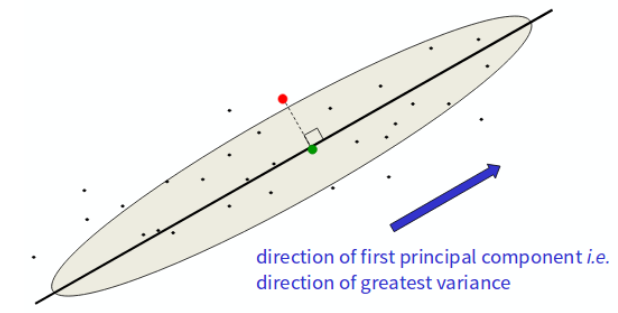
\includegraphics[width=\linewidth]{images/PCA.png}
    \label{fig:Scaled Dot Product Attention}
    \vspace{-10pt}
\end{wrapfigure}
PCA learns an \textbf{orthogonal, linear transformation} of the data that projects an input $\mathbf{x}$ to a \textbf{low-dimensional representation $\mathbf{z}$}, which lies in the subspace spanned by the \textbf{principal components}.
PCA works well \textbf{only} if the data is near a \textbf{linear manifold} in high-dimensional space.
We are interested in learning representations that \textbf{disentangle} more \textbf{complicated forms of feature dependencies}.
For this purpose, we need more than what can be done with a \textbf{simple linear transformation}.

\subsection{An inefficient way to fit PCA}
\begin{wrapfigure}{r}{0.4\textwidth}
    \centering
    \vspace{-10pt}
    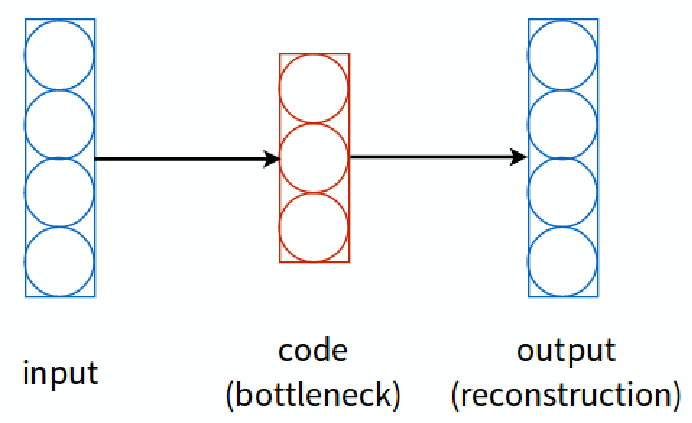
\includegraphics[width=\linewidth]{images/Bottleneck_layer.png}
    \label{fig:An inefficient way to fit PCA}
    \vspace{-10pt}
\end{wrapfigure}
The idea is to train a neural network with a \textbf{"bottleneck" hidden layer} having $M$ units and try to make the output ($\hat{\mathbf{x}}$) the same as the input ($\mathbf{x}$).
If the hidden and output layers are \textbf{linear}, and we minimize the squared reconstruction error:
\[
\min \left\| \hat{\mathbf{x}} - \mathbf{x} \right\|^2
\]
The $M$ hidden units will span the \textbf{same subspace} as the first $M$ principal components.
However:
\begin{compactitemize}
    \item Their \textbf{weight vectors} will \textbf{not be orthogonal}.
    \item They will have approximately \textbf{equal variance}.
\end{compactitemize}

\section{Autoencoders}
\begin{wrapfigure}{r}{0.4\textwidth}
    \centering
    \vspace{-10pt}
    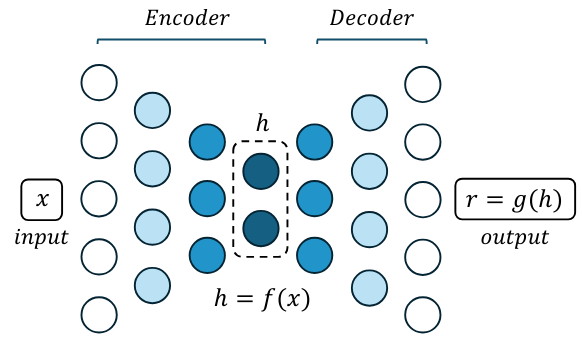
\includegraphics[width=\linewidth]{images/autoencoder+.png}
    \label{fig:Scaled Dot Product Attention}
    \vspace{-10pt}
\end{wrapfigure}
An \textbf{autoencoder} is a feed-forward neural network trained to attempt to copy its input to its output.
The network may be viewed as a consisting of two parts: an \textbf{encoder} function $h=f(x)$ and a \textbf{decoder} that produces a reconstruction $r=g(h)$.
The aim is to induce in $h$ useful properties and the most salient features of the training data.

\begin{figure}[H]
    \centering
    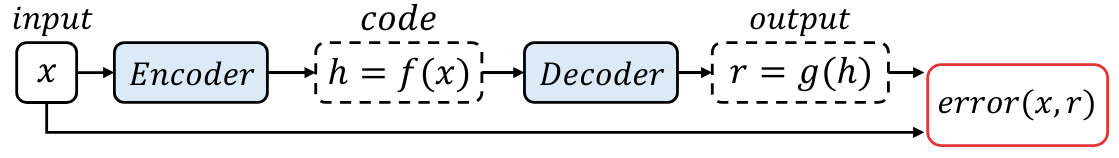
\includegraphics[width=0.6\textwidth]{images/autoendoer_pipeline.png}
    \caption{Autoencoders Pipeline}
    \label{fig:MHA2}
\end{figure}
\newpage
With \textbf{nonlinear layers} before and after the code , it should be possible to represent data on or near a \textbf{nonlinear manifold}. The \textbf{encoder} maps from the data space ($\mathbf{x}$) to the \textbf{coordinates on the manifold} ($\mathbf{z}$). The \textbf{decoder} performs the \textbf{inverse transformation} ($\hat{\mathbf{x}}$). Both the encoder and the decoder can be rich, \textbf{multi-layer functions}.

\subsection{Risk: Learning the Identity Function}
\begin{wrapfigure}{r}{0.25\textwidth}
    \centering
    \vspace{-10pt}
    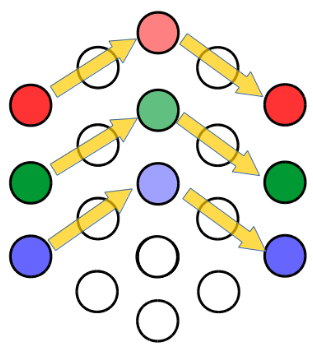
\includegraphics[width=\linewidth]{images/identity.png}
    \label{fig:Scaled Dot Product Attention}
    \vspace{-10pt}
\end{wrapfigure}
What we mean by \textbf{overfitting} in autoencoders is slightly different from classic Neural Networks (NNs). Here, the risk is not merely memorizing every single data point, but rather learning a trivial function that maps $g(f(\mathbf{x}))=\mathbf{x}$ everywhere.
Therefore, the model does not effectively \textbf{compress} the data; it simply \textbf{copies} the input to the output.
This eventually can occur if the encoder and decoder are given \textbf{too much capacity} (e.g., if the hidden layers are too large or deep), or if the hidden code has a dimension \textbf{greater than the input} (an overcomplete code), which facilitates the learning of the identity function.

\subsection{Undercomplete Autoencoders}
The first attempt at autoencoder regularization is to constrain $h$ to have a \textbf{smaller} dimension than $x$.
Learning an \textbf{undercomplete} representation forces the autoencoder to capture the most salient factors of data variation.
The learning process plans to minimize:
\begin{equation}
    L(x,g(f(x)))
\end{equation}
where $L$ is a loss function penalizing $g(f(x))$ for being dissimilar from $x$ (e.g. MSE).

\textbf{Problem}: if the encoder and decoder are allowed too much capacity, an undercomplete autoencoder can learn to perform the copying task without extracting useful information.
\begin{figure}[H]
    \centering
    \begin{minipage}{0.45\textwidth}
        \centering
        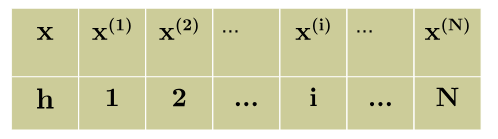
\includegraphics[width=\textwidth]{images/UA2.png}
        \label{fig:Trend_Seasonality}
    \end{minipage}
    \hfill
    \begin{minipage}{0.45\textwidth}
        \centering
        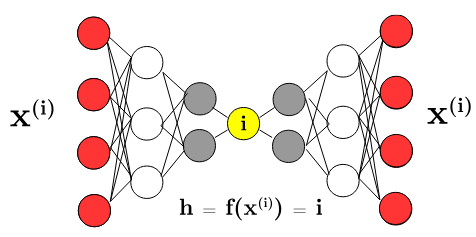
\includegraphics[width=\textwidth]{images/UA.png}
        \label{fig:Residuals}
    \end{minipage}
    \label{fig:TS_Residuals}
\end{figure}

\section{Regularized Autoencoders}
The fundamental tension in autoencoder design parallels general machine learning: insufficient capacity causes underfitting, while excessive capacity enables learning the identity function. Deep learning principles suggest using large models with sufficient capacity to fit complex functions, but constraining them through regularization to use this power wisely. 
Regularized autoencoders use a loss function that encourages the model to have other properties besides tha ability to copy its input to its output.
Beacause the model is \textbf{forces to prioritize} which aspects of the input should be copied, it often learns \textbf{useful properties} of the data.
It can capture the structure of the data-generating distribution due to \textbf{opposition} between reconstruction distribution and regularizer.


\subsection{Sparse Autoencoders} 
\begin{wrapfigure}{r}{0.25\textwidth}
    \centering
    \vspace{-10pt}
    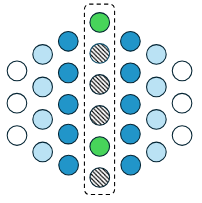
\includegraphics[width=\linewidth]{images/SA.png}
    \label{fig:Scaled Dot Product Attention}
    \vspace{-10pt}
\end{wrapfigure}
A \textbf{sparse autoencoder} is an autoencoder whose training criteretion involves an additional \textbf{sparsity penalty} on the code layer $h$. 
\begin{equation} L_{SAE} = D(x, g(f(x))) + \lambda \|h\|_{1} \end{equation} 
Thanks to the sparsity penalty, we can build an over-complete representation of the input data without the risk of learning the identity function. Sparse autoencoders are typically used to learn features for another rask, such as \textbf{classification}.


\begin{infobox}[Where the regularization is applied?]
    In a sparse autoencoder, the regularization is applied \textbf{directly on the activations of the code layer $h$}, not on the weights. This differs from typical weight regularization (like $L_1$ or $L_2$ penalties on $W$), which constrains the magnitude of the parameters. 
    
    By penalizing the activations instead, the model is forced to activate only a few neurons for each input, learning a \textbf{sparse representation} even if the network has many hidden units.
\end{infobox}
    
\begin{infobox}[The size of code layer]
    The code layer $h$ in a sparse autoencoder is often \textbf{larger than the input layer}, creating an \textbf{over-complete representation}. 
    
    Even though there are more neurons than input dimensions, the sparsity penalty ensures that for each input, only a small subset of neurons is active. This allows the autoencoder to learn richer, more disentangled features without simply copying the input.
\end{infobox}
\begin{wrapfigure}{r}{0.35\textwidth}
    \centering
    \vspace{-10pt}
    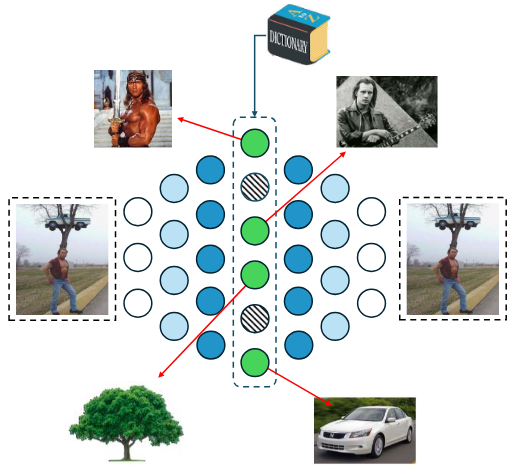
\includegraphics[width=\linewidth]{images/SA_idea.png}
    \label{fig:Scaled Dot Product Attention}
    \vspace{-10pt}
\end{wrapfigure}
Sparse autoencoders can discover representa-tions that account for most or all information on a signal with a combination of a small num-ber of elementary, recurrent, and only partially related concepts.
Given the input signal, the general idea is to find a short list of terms that best describes the input from a \textbf{learned dictionary}.
The new representation h has the dimensionality of the dictionary, much higher than the dimen- sionality of the input (overcompleteness)

\subsection{Denoising Autoencoders}
\begin{wrapfigure}{r}{0.4\textwidth}
    \centering
    \vspace{-10pt}
    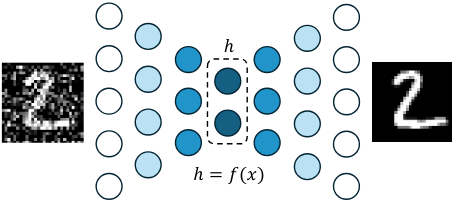
\includegraphics[width=\linewidth]{images/DA.png}
    \label{fig:Scaled Dot Product Attention}
    \vspace{-10pt}
\end{wrapfigure}
To force to discover more \textbf{robust features}, a \textbf{denoising autoencoder} reconstruct the input $x$ from a  \textbf{corrupted version} $\hat{x}$ of it.
\begin{equation}
    L_{DAE}=D(x,g(f(\hat{x}))) e.g., \hat{x} \sim N(x,\sigma^2 I)
\end{equation}
The corrupted input $\hat{x}$ can be obtained by applying on $x$ some form of noise, for example, additive white gaussian noise or dropout.

Denoising autoencoders must therefore \textbf{undo} this corruption rather than simply copying their input.

\begin{infobox}[The size of code layer]
    In Denoising Autoencoders, unlike Sparse Autoencoders, the number of neurons in the code layer is usually smaller than the input layer. 
    This is because each neuron in the code layer is activated by the input, and having a code larger than the input could lead the model to simply learn the identity function.
\end{infobox}

\begin{wrapfigure}{r}{0.5\textwidth}
    \centering
    \vspace{-10pt}
    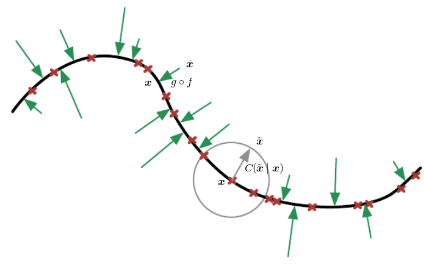
\includegraphics[width=\linewidth]{images/FV.png}
    \label{fig:Scaled Dot Product Attention}
    \vspace{-10pt}
\end{wrapfigure}
A \textbf{Denoising Autoencoder (DAE)} is able to bring $\hat{x}$ back to the ``curve'' point 
where the original $x$ resides. In other words, it \textbf{learns a vector field towards higher probability regions}. 

By knowing, for each point near the curve, where it should be projected, a DAE has \textbf{implicitly learned the structure of the underlying manifold} responsible for the data-generating process. 

The \textbf{denoising training} forces the encoder and decoder to \textbf{implicitly capture the structure of the probability distribution} $p_{\text{data}}(x)$.

\subsubsection{Denoising Autoencoders for Anomaly Detection}
\textbf{Denoising Autoencoders (DAE)} learn to reconstruct samples that lie on the \textbf{data manifold} by removing noise from the input.

\textbf{Key insight:} During training, the model learns the \textbf{typical structure of normal data}. 
When presented with an \textbf{anomalous sample}, its reconstruction error becomes significantly higher, because the anomaly does not lie on the learned manifold.

\textbf{DAEs for Anomaly Detection: how they work:}
\begin{compactitemize}
    \item Train the DAE with \textbf{noisy versions of normal data}.
    \item At inference, compute the \textbf{reconstruction error} $e(x) = \|x - \hat{x}\|_2$.
    \item Flag samples with \textbf{high $e(x)$} as potential anomalies.
\end{compactitemize}

\subsection{Contractive Autoencoders}
A \textbf{contractive autoencoder} is an autoencoder that reconstructs the input from the code and makes the \textbf{code insensitive} to the input.
\begin{equation}
    L_{CAE} = D(x, g(f(x))) + \lambda \left\| \frac{\partial f(x)}{\partial x} \right\|_2
\end{equation}
The regularization term encourages the gradient of the hidden layer with respect to inputs to be small. This forces the model to:
\begin{compactitemize}
    \item learn a function that \textbf{does not change much} when $x$ changes slightly or is affected by small perturbations.
    \item reduces the number of effective degrees of freedom of the representation.
    \item represent only the variations that are needed to reconstruct training examples.
\end{compactitemize}

\vspace{0.2cm}
\begin{wrapfigure}{r}{0.4\textwidth}
    \centering
    \vspace{-10pt}
    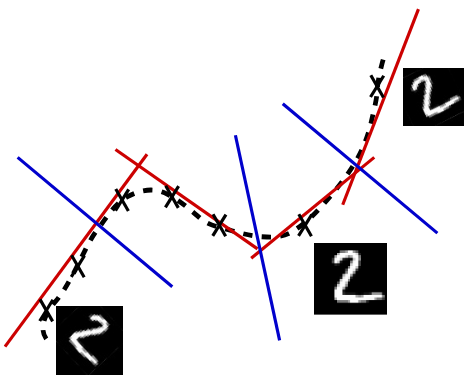
\includegraphics[width=\linewidth]{images/CA.png}
    \label{fig:Scaled Dot Product Attention}
    \vspace{-10pt}
\end{wrapfigure}
We wish to extract features that only reflect variations observed in the training set.

With the \textcolor{red}{red line}, we indicate directions of variations for which the encoder needs to be sensitive to reconstruct well input.

With the \textcolor{blue}{blue line} line, we indicate directions of variations for which the encoder doesn’t need to be sensitive because they are not observed in the training set.

The name \textbf{Contractive Autoencoder (CAE)} arises from the way that the CAE \textbf{warps space}. 
Because the CAE is trained to \textbf{resist perturbations of its input}, it is encouraged to map a neighborhood of input points to a \textbf{smaller neighborhood of output points}. 
Thanks to the \textbf{contractive term}, the model becomes \textbf{invariant to small perturbations} near the points.

As is the case for \textbf{Denoising Autoencoders}, a CAE knows the \textbf{tangent planes} at each location of the underlying manifold. 
In this way, it can \textbf{capture the manifold structure of the data}.

\chapter{Generative models}

\section{Variational Autoencoders}
Generative modeling is an area of machine learning that deals with models of distributions $p(x)$, defined over datapoints $x$ in some potentially high-dimensional space $\mathcal{X}$. 
Unlike the previous autoencoder model, here we do not aim to learn a compact representation of the input and then reconstruct it. Instead, we want to learn the probability distribution of the data, that is, the probability of each element in the dataset.

There are two main reasons for doing this:
\begin{compactitemize}
    \item \textbf{Sampling}: if we know the data distribution, we can sample from it to generate new data.
    \item \textbf{Anomaly Detection}: after training, we can evaluate the probability of a given datapoint under the learned distribution. If the probability is high, we can consider the datapoint as "normal"; if it is low, the datapoint is likely to be different in some way, and thus considered anomalous.
\end{compactitemize}

\subsection{The problem of the distribution and the Latent Variables}
\begin{wrapfigure}{r}{0.25\textwidth}
    \centering
    \vspace{-10pt}
    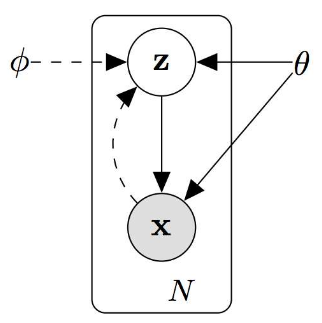
\includegraphics[width=\linewidth]{images/latent_variable_model.png}
    \label{fig:Scaled Dot Product Attention}
    \vspace{-10pt}
\end{wrapfigure}
Typically, we work with complex data (e.g., images), so using a very simple distribution (such as a normal distribution) to represent our data can be inefficient.
Taking a step back, denoising autoencoders and contractive autoencoders implicitly learn the structure of the probability distribution p(x), but sampling new examples from these models is very complex because the learned distribution is encoded implicitly in the network weights and there is no defined sampling mechanism.
Therefore, we would ideally like to have a distribution $p(x)$ that is simple enough to allow efficient sampling, yet expressive enough to represent our data in a realistic way. The key idea is to map our data into another space where a simple distribution is sufficient, and then map samples drawn from this simple distribution back to the original data space. 
This concept is known as \textbf{Latent Variable Models}. Essentially, we model the probability of the observable data based on some underlying variables (called latent variables) that are not directly observable. These latent variables capture hidden characteristics of the data and allow us to describe complex distributions using simpler ones.

\subsection{Latent Variables in Weather Modeling}
\begin{wrapfigure}{r}{0.3\textwidth}
    \centering
    \vspace{-10pt}
    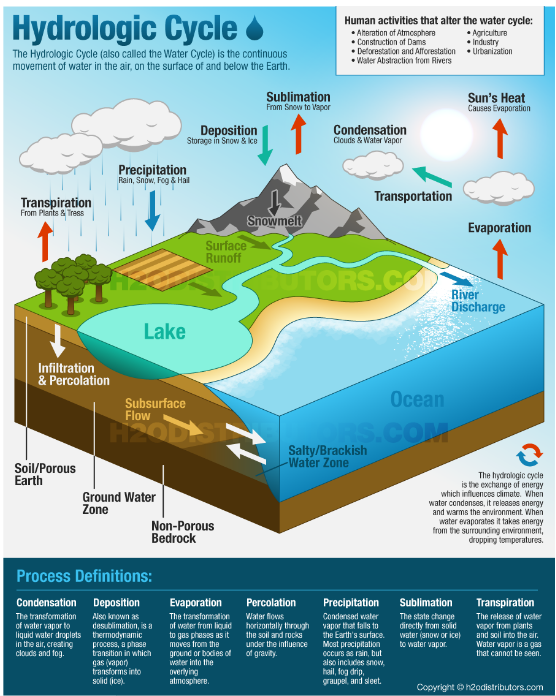
\includegraphics[width=\linewidth]{images/WM.png}
    \label{fig:Scaled Dot Product Attention}
    \vspace{-10pt}
\end{wrapfigure}
The idea in this examples is that latent variables can represent hidden physical quantities that exaplain observable data.
We can measure quantities like temperature, humidity, and wind speed. However, these depend on other \textbf{unobserved pysical factors} like:
\begin{compactitemize}
    \item pressure gradients in the atmosphere
    \item altitude temperature profiles
    \item vapor concentration and cloud density
\end{compactitemize}
These hidden quantities form the \textbf{latent variables} $z$.
They govern the observable weather data $x$, even if we cannot measure them directly.


\subsection{Latent Variable Models}
Latent Variable Models relate a set of \textbf{observable} variables $x$ to a set of \textbf{latent} (hidden) variables $z$.  
The latent variables represent underlying factors that are not directly observable, but that influence the formation of the data.

We assume that the data $x$ is generated from some latent variable $z$, therefore:
\[
p(x, z) = p(x \mid z)\, p(z),
\]
where:
\begin{itemize}
    \item $p(z)$ is the \textbf{prior distribution} of the latent variables (typically chosen to be simple, e.g., a Gaussian),
    \item $p(x \mid z)$ is the \textbf{generative model}, describing how data $x$ is generated from $z$.
\end{itemize}

Since $z$ is not observed, the probability distribution of the observable data $x$ is obtained by \textbf{marginalizing} over $z$:
\[
p(x) = \int p(x, z)\, dz = \int p(x \mid z)\, p(z)\, dz.
\]

This follows from:
\begin{itemize}
    \item \textbf{Law of Total Probability}: $\displaystyle p(x) = \int p(x, z)\, dz$,
    \item \textbf{Definition of Conditional Probability}: $\displaystyle p(x, z) = p(x \mid z)\, p(z)$.
\end{itemize}

The integral
\[
p(x) = \int p(x \mid z)\, p(z)\, dz
\]
is often \textbf{intractable} in closed form, especially when $z$ has high dimensionality or the model is complex.  
This is one of the central challenges in Bayesian statistics and probabilistic machine learning.

A practical way to approximate $p(x)$ is through Monte Carlo sampling:
\[
p(x) \approx \frac{1}{K} \sum_{k=1}^{K} p(x \mid z^{(k)}), \qquad z^{(k)} \sim p(z).
\]

The sampling procedure is:
\begin{enumerate}
    \item Sample a latent variable: $z \sim p(z)$,
    \item Generate an observation: $x \sim p(x \mid z)$.
    \item Apply Monte Carlo approximation $z \rightarrow x.$
\end{enumerate}

\subsection{Problem with Monte Carlo}
The monte carlo approximation heavly depends of which sample has been sampled by $p(z)$, and we need a large number of sample to get a good estimate of $p(x)$ and most of $z$'s sampled are irrelevant for the specific observation of $x$.

The idea to solve this problem is learn a model that, given an observation $x$, predicts the most \textbf{plausible latent variables} $z$, those that are \textbf{more likely related} to $x$ under the true posterior distribution $p(z|x)$.

\subsection{Variational Inference}

Variational Inference is a framework used to approximate intractable posterior distributions.  
The central idea is to replace the true posterior distribution $p(z \mid x)$, which is often complex and computationally expensive, with a simpler and tractable distribution $q(z \mid x)$, called the \textbf{Proposal distribution} or \textbf{approximate posterior}.

The goal is to choose a family of distributions $q(z \mid x)$ that is:
\begin{compactitemize}
    \item expressive enough to approximate $p(z \mid x)$ well,
    \item but simple enough to evaluate and to sample from efficiently.
\end{compactitemize}

This allows us to approximate integrals of the form:
\[
p(x) = \int p(x \mid z)\, p(z)\, dz,
\]
using a small number of meaningful samples drawn from $q(z \mid x)$ rather than from $p(z)$.

The objective of variational inference is therefore to find (or learn) the approximate posterior:
\[
q^\ast(z \mid x) \approx p(z \mid x).
\]

A common way to define this objective is to minimize the Kullback–Leibler divergence between the two distributions:
\[
q^\ast(z \mid x)
= \arg\min_{q} \, D_{\mathrm{KL}}\bigl(q(z \mid x)\, \Vert\, p(z \mid x)\bigr).
\]

However, directly minimizing this divergence requires evaluating $\log p(x)$, which is generally \textbf{intractable} for complex generative models.  
This motivates the introduction of the \textbf{Evidence Lower Bound (ELBO)}, which provides a computable objective that indirectly minimizes the KL divergence.

Start with tha calulus:
\begin{align}
    q^*(z \mid x) 
    &= \arg\min_q \, D_{\mathrm{KL}}\!\left[q(z \mid x) \;\Vert\; p(z \mid x)\right] \\
    &= \mathbb{E}_{z \sim q(z \mid x)} \left[ \log q(z \mid x) - \log p(z \mid x) \right] \\
    &= \mathbb{E}_{z \sim q(z \mid x)} \left[ \log q(z \mid x) - \log \frac{p(x \mid z)\, p(z)}{p(x)} \right] \\
    &= \mathbb{E}_{z \sim q(z \mid x)} \left[ \log q(z \mid x) - \log p(x \mid z) - \log p(z) + \log p(x)\right] \\
    &= \mathbb{E}_{z \sim q(z \mid x)} \left[ \log q(z \mid x) - \log p(x \mid z) - \log p(z)\right] + \log p(x) \\
    &= \mathbb{E}_{z \sim q(z \mid x)} \left[ \log q(z \mid x) - \log p(z)\right] - \mathbb{E}_{z \sim q(z \mid x)} \left[\log p(x \mid z)\right] + \log p(x) \\
    &= D_{\mathrm{KL}} \left[q(z \mid x) \mid \mid p(z)\right] - \mathbb{E}_{z \sim q(z \mid x)} \left[\log p(x \mid z)\right] + \log p(x)
\end{align}
The equation can be written like this:
\[
\log p(x) - \color{blue} D_{\mathrm{KL}} \big[q(z \mid x) \, \Vert \, p(z \mid x)\big]
\color{black}=
\color{red}{\mathbb{E}_{z \sim q(z \mid x)}[\log p(x \mid z)] - D_{\mathrm{KL}} \big[q(z \mid x) \, \Vert \, p(z)\big]}
\]
Where:
\begin{compactitemize}
    \item the part in red is the \textbf{ELBO}, that is something that can we optimize using the  stochastic gradient descent given the right choice of $q()$.
    \item the part in blue is allways positive and is the KL divergence between the proxy and the real posterior distributions.
\end{compactitemize}

\begin{infobox}[Note]
    The equation above is important beacuse provides a relationship between $p(x)$ and the posterior distribution $q(z|x)$
\end{infobox}

So now we can write the equation like this:
\[
\log p(x) = D_{\mathrm{KL}} \big[q(z \mid x) \, \Vert \, p(z \mid x)\big] + \mathrm{ELBO}
\]
Since the $D_{KL}$ term is always non-negative, this leads to the following inequality:
\[
\log p(x) \ge \mathrm{ELBO}, \quad \text{where} \quad 
\mathrm{ELBO} = \mathbb{E}_{z \sim q(z \mid x)}[\log p(x \mid z)] 
- D_{\mathrm{KL}} \big[q(z \mid x) \, \Vert \, p(z)\big]
\]
\begin{wrapfigure}{r}{0.45\textwidth}
    \centering
    \vspace{-10pt}
    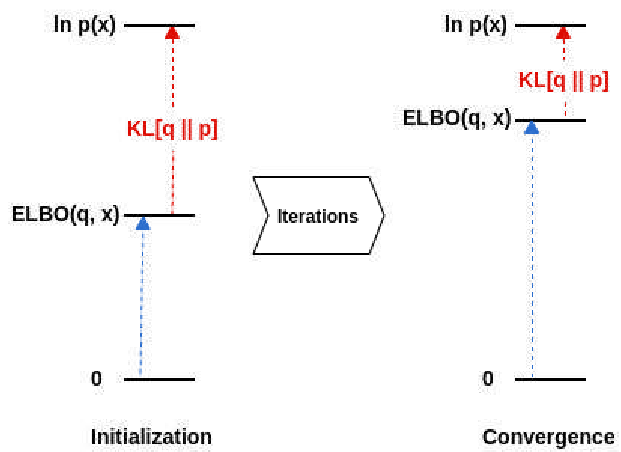
\includegraphics[width=\linewidth]{images/ELBO.png}
    \label{fig:Scaled Dot Product Attention}
    \vspace{-10pt}
\end{wrapfigure}
Results:
\begin{compactitemize}
    \item Maximizing the ELBO provides a lower bound on the true log-likelihood $\log p(x)$.
    \item Therefore, maximizing the ELBO is equivalent to making our model as close as possible to the true data distribution.
    \item If we maximize the ELBO, we simultaneously minimize the KL divergence between the true intractable posterior and the proposal/posterior (our initial goal).
\end{compactitemize}

\subsection{Variational Autoencoder: the Encoder and the Decoder}
A Variational Autoencoder (VAE) is an autoencoder trained to maximize the \textbf{Evidence Lower Bound (ELBO)}:

\[
\mathrm{ELBO} = \underbrace{\mathbb{E}_{z \sim q_\phi(z \mid x)}[\log p_\theta(x \mid z)]}_{\text{Reconstruction Term}}
- \underbrace{D_{\mathrm{KL}}\big[q_\phi(z \mid x) \, \Vert \, p(z)\big]}_{\text{Regularization Term}}
\]
\textbf{Components of the VAE:}
\begin{itemize}
    \item \textbf{Encoder network} $q_\phi(z \mid x)$: given an input $x$, it outputs a distribution (typically Gaussian) that approximates the true posterior $p(z \mid x)$.
    \begin{compactitemize}
        \item Unlike a standard autoencoder, the encoder does not output a deterministic vector, but the parameters (mean and variance) of a latent distribution.
        \item Formally: $x \to f_{\text{ENC}}(x; \phi) = [\mu(x), \sigma^2(x)]$, such that $z \sim \mathcal{N}(\mu(x), \sigma^2(x))$.
        \item In practice, the encoder outputs two vectors, $\mu(x)$ and $\sigma^2(x)$, representing the mean and variance of the approximate posterior.
    \end{compactitemize}
    \item \textbf{Decoder network} $p_\theta(x \mid z)$: reconstructs the input $x$ from a sampled latent variable $z$, modeling the likelihood of the data.
    \begin{compactitemize}
        \item The decoder takes a latent variable $z$ sampled from the encoder $q(z \mid x)$ and produces a reconstruction $x_{\text{recon}}$.
        \item Formally: $x_{\text{recon}} \to g_{\text{DEC}}(z; \theta)$, where $z \sim \mathcal{N}(\mu(x), \sigma^2(x))$.
        \item The decoder aims to maximize the conditional log-likelihood $\log p(x \mid z)$.
        \item In practice, for continuous data, this is often implemented by minimizing the Mean Squared Error (MSE) between the original input $x$ and the reconstruction $x_{\text{recon}}$.
    \end{compactitemize}    
\end{itemize}

Now take a look at the \textbf{regularization term}: we say that
\begin{compactitemize}
    \item $D_{\mathrm{KL}}[q(z \mid x) \, \Vert \, p(z)]$ is a measure of how $q(z \mid x)$ diverges from the distribution $p(z)$, called the \emph{prior distribution}.  
    \item $p(z)$ is the expected probability distribution over the latent variable; it is hand-crafted and typically follows a standard Gaussian distribution.  
    \item If both posterior and prior distributions have Gaussian form (as holds in this case), the $D_{\mathrm{KL}}$ has a closed-form equation.
\end{compactitemize}

\begin{figure}[H]
    \centering
    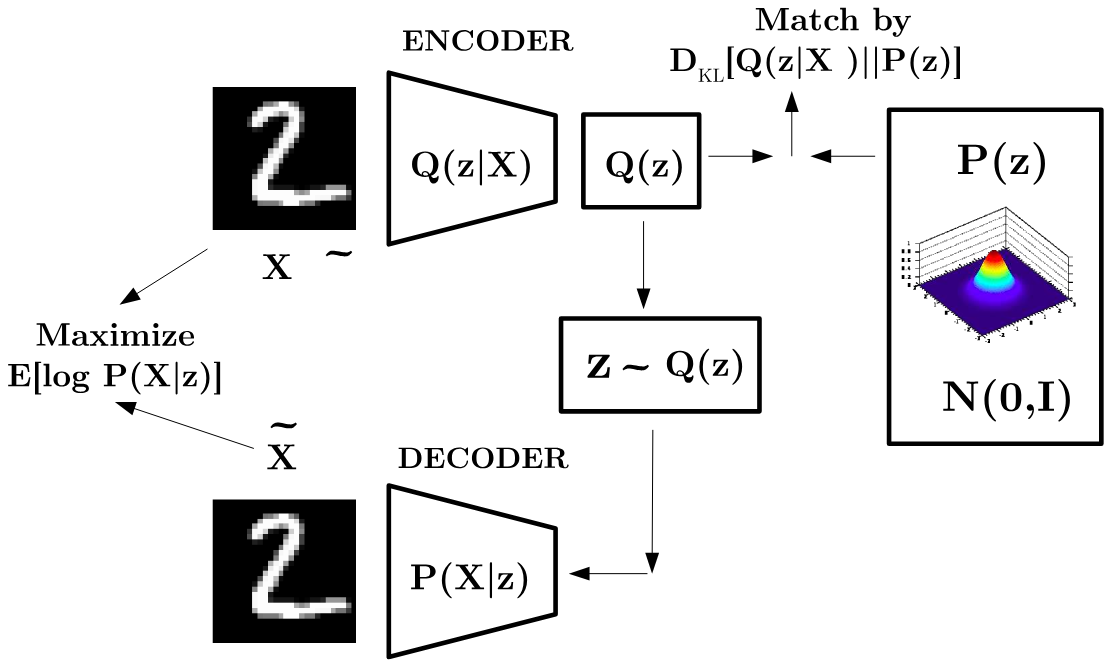
\includegraphics[width=0.5\textwidth]{images/VAE.png}
    \caption{Variational Autoencoders: overall architecture}
    \label{fig:MHA2}
\end{figure}

\subsection{The reparametrization trick}
\begin{wrapfigure}{r}{0.4\textwidth}
    \centering
    \vspace{-10pt}
    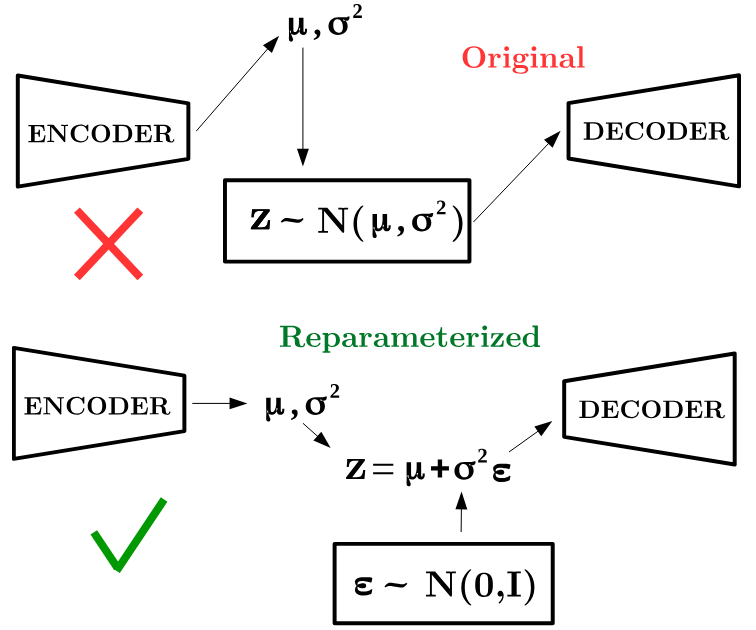
\includegraphics[width=\linewidth]{images/RP.png}
    \label{fig:Scaled Dot Product Attention}
    \vspace{-10pt}
\end{wrapfigure}
The sampling step $z \sim N(z \mid \mu(x), \sigma^2(x))$ is not differentiable, so we can not use the backpropagation to train the model.
The \textbf[reparametrize trick] lets us backpropagate through the sampling operation (a random operator). So instead of do $z \sim N(z \mid \mu(x), \sigma^2(x))$  we compute this:
\begin{compactitemize}
    \item Sample a random vector from the standard distribution $\epsilon \sim N(z \mid 0, I_n)$
    \item \textbf{Reparametrize}: $z= \mu(x) + \epsilon * \sigma(x)$
\end{compactitemize}
The advantage is that the sampled noise vector $\epsilon$ is just an extra input to the network. Its distribution is not a function of any of the variables whose derivatives we want to calculate, which allows gradients to flow through the network during backpropagation.

\section{Generative Adversarial Networks}
\chapter{Discrete Representations and Generative Modeling}

\section{Introdcution}
The \textbf{Discretization} is the process of dividing continuos phenomena into \textbf{distinct parts}, resonates deeply with how humans understand and interact with the world.

It is not just a computational tool but a reflection of a fundamental cognitive process. It has been explored in philosopy, science, and mathematics for centuries.

\subsection{Immanuel Kant}
Philosophers have long pondered how humans make sense of the
continuous and often chaotic flow of reality.
\begin{wrapfigure}{r}{0.2\textwidth}
    \centering
    \vspace{-10pt}
    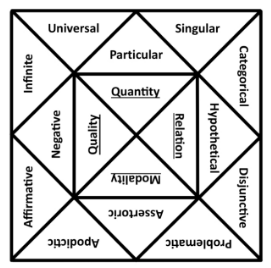
\includegraphics[width=\linewidth]{images/Kant.png}
    \label{fig:Scaled Dot Product Attention}
    \vspace{-10pt}
\end{wrapfigure}
\textbf{Immanuel Kant}, in his seminal Critique of Pure Reason (1781), argued
that the human mind does not passively receive sensory input but actively
structures it.

According to Kant, this structuring process involves applying innate \textbf{categories of understanding} to the manifold of experience – a form of \textbf{conceptual discretization}, to borrow a modern term, that transforms raw sensory data into coherent and intelligible knowledge.

\subsection{René Descartes}
Similarly, René Descartes revolutionized mathematics and philosophy by introducing the Cartesian coordinate system in his 1637 work La Géométrie.
\begin{wrapfigure}{r}{0.2\textwidth}
    \centering
    \vspace{-10pt}
    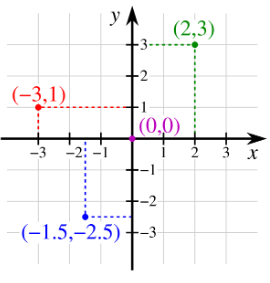
\includegraphics[width=\linewidth]{images/renè.png}
    \label{fig:Scaled Dot Product Attention}
    \vspace{-10pt}
\end{wrapfigure}
By discretizing continuous space into measurable dimensions of x and y, Descartes laid the groundwork for modern analytical geometry.

This act of partitioning space into discrete points not only enabled scientific progress but also reflected a deeper philosophical position: that understanding the infinite requires reducing itto finite, manageable parts.

\subsection{Why Discrete Representations?}
Many real-world domains are inherently \textbf{discrete}, and modeling them with continuous representation may miss important structural properties. For example like:
\begin{compactitemize}
    \item \textbf{Language} consist of sequence of discete symbols (word, subword).
    \item \textbf{Images} are stored as discrete grids of pixels with quantized color values.
    \item \textbf{Music and speech} are often represented symbolically (e.g, notes, phonemes).
\end{compactitemize}


In the context of artificial learning systems, dicrete models and representation/enable:
\begin{compactitemize}
    \item \textbf{Efficient Compression}
    Discrete latent variables are significantly \textbf{easier to encode compactly}. This facilitates better data compression and representation efficiency, as the information is stored using distinct, finite codes.
    
    \item \textbf{Symbolic Reasoning}
    Discrete representations enable the direct application of \textbf{formal logic} and \textbf{symbolic manipulation}. This is crucial for tasks requiring transparent, step-by-step reasoning, such as applying mathematical or logical rules.

    \item \textbf{Modular Design}
    Discrete mechanisms facilitate the creation of \textbf{modular and specialized architectures}. In systems like the \textbf{Mixture of Experts (MoE)}, a discrete gating function selects specific experts for computation, leading to:
\end{compactitemize}
\begin{figure}[H]
    \centering
    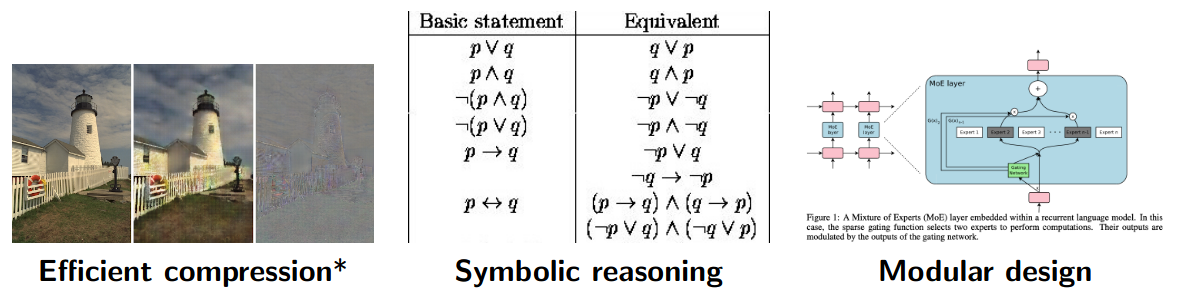
\includegraphics[width=0.9\textwidth]{images/D1.png}
    \label{fig:MHA2}
\end{figure}

\subsection{Problem with descritization}
So if we say since the beginning of the course, each NN is trained through gradient descent, this implies that each function that we use is differentiable.

But many times when we do discretization, we use functions like argmax or argmin that clearly are not differentiable functions. To give an example, if we try to run the code showed below, it won't run because we cannot compute the gradient of the argmax function.
\begin{figure}[H]
    \centering
    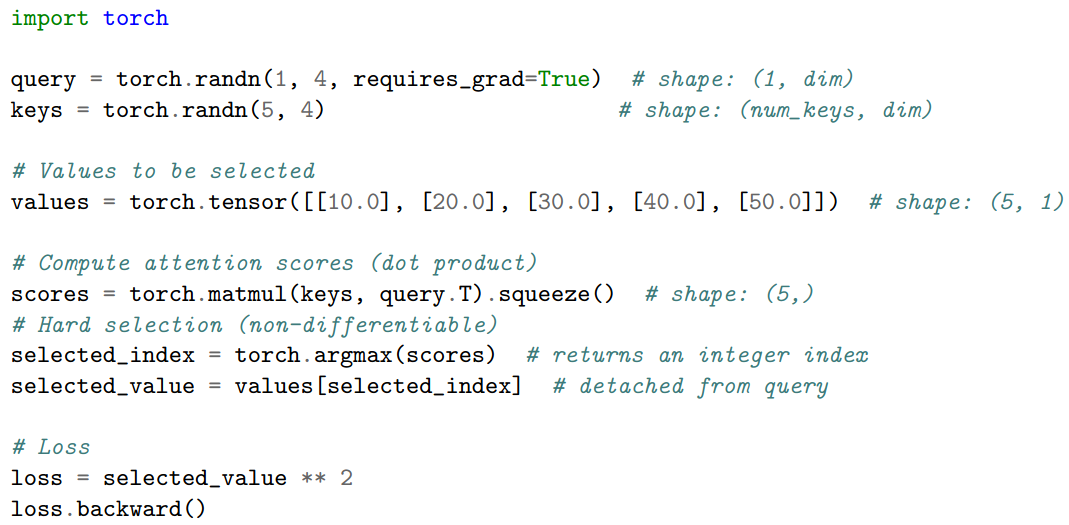
\includegraphics[width=0.9\textwidth]{images/code.png}
    \label{fig:MHA2}
\end{figure}

A possible solutions for this problem are:
\begin{compactitemize}
    \item \textbf{VQ-VAEs} involve straight-through estimators
    \item \textbf{Pixel-RNN} employ autoregressive training
    \item Surrogate gradients (e.g., Gumbel Softmax)
\end{compactitemize}

\section{Vector Quantized-Variational Autoencoders}
While Variational Autoencoders (VAEs) are effective at learning a compressed, lower-dimensional representation of the training data and providing an explicit density estimation for generating new samples, they suffer from two major problems.

The most noticeable issue is their tendency to generate \textbf{blurry}, unrealistic outputs. This is because VAEs typically use a pixel-wise reconstruction loss (like Mean Squared Error), which penalizes variance and tends to favor an average of possible outputs rather than sharp, high-frequency details. This averaging effect results in blurry images.
\begin{figure}[H]
    \centering
    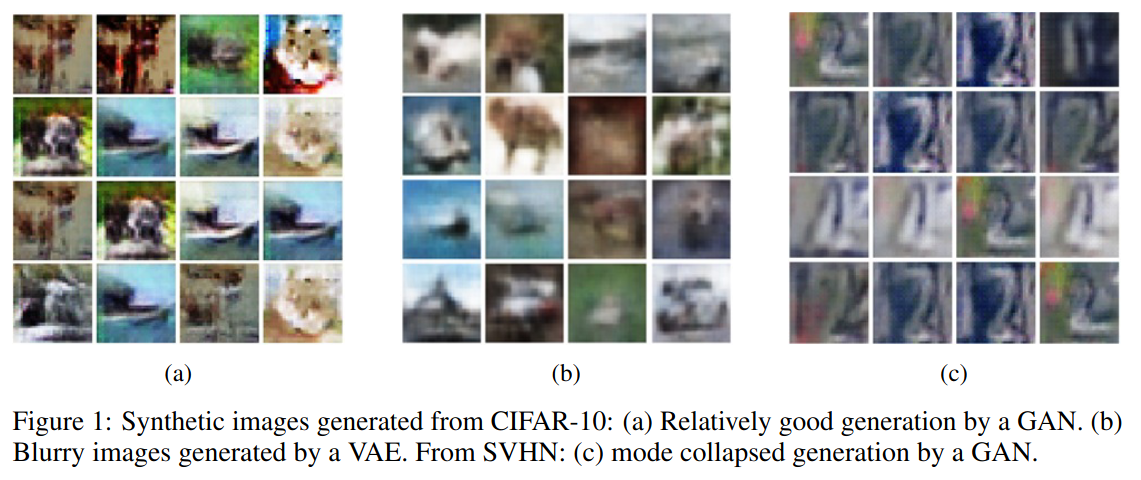
\includegraphics[width=0.8\textwidth]{images/D2.png}
    \label{fig:MHA2}
\end{figure}
The second core issue is \textbf{Posterior Collapse}. This occurs when the encoder's variational posterior distribution collapses quickly to the prior distribution (often a simple Gaussian) early in the training process. When this happens, the latent variables (z) essentially stop carrying any meaningful information about the input image (x), effectively making the generative process redundant. Consequently, the decoder learns to ignore the latent code and generates images based solely on the overall structure of the training dataset. This collapse is often difficult to reverse; once the encoder has settled on the uninformative prior, it rarely recovers without specific interventions or architectural changes.

The are two possbile solutions:
\begin{compactitemize}
    \item \textbf{$\beta-VAE$} it simply introduces a hyperparameters $\beta$ to weigh the importance of the KL divergence within the ELBO objective:
    \[
        \mathcal{L}_{\text{VAE}} = \mathbb{E}_{z \sim Q(z|X)}[\log P(X|z)] - \beta D_{KL}[Q(z|X)\|P(z)]
    \]
    \item \textbf{Vector Quantized-Variational Autoencode}
\end{compactitemize}

\subsection{Vector Quantized-Variational Autoencode (VQ-VAE)}
VQ-VAE is the first model to use \textbf{discrete latent variables} successfully, it uses the whole latent space and avoids the posterior collapse problem.

VQ-VAE is a \textbf{standard} autoencoder network, with an ancoder and a decoder network. Differently from VAEs, the latent embedding space does \textbf{not follow a Gaussian distribution}.

The model takes an input $x$, that is passed through an encoder network, the encoder produces a \textbf{continuos} output $z_e(x)$.
\begin{wrapfigure}{r}{0.5\textwidth}
    \centering
    \vspace{-10pt}
    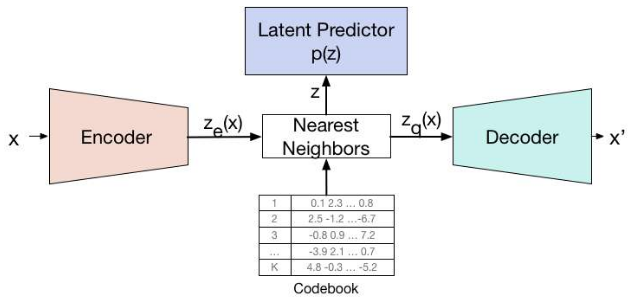
\includegraphics[width=\linewidth]{images/VQ1.png}
    \label{fig:Scaled Dot Product Attention}
    \vspace{-10pt}
\end{wrapfigure}
The latent space is defined through a \textbf{learnable} lookup table, also called \textbf{codebook}, $e \in R^{KxD}$.

$K$ is the size of the discrete latent space and $D$ is the dimensionality of each latent embedding vector. Hence, the codebook is $KxD$.

Each of the $K$ embedding vectors $e_i \in R^D, i=1,2, ... , K$ is learnable through gradient descent.

Given $z_e(x)$, the discrete latent variable $z$ is computed by a \textbf{nearest neighbour look-up} using the shared embedding space.
$$q(z = k|x) =
\begin{cases}
1 & \text{se } k = \underset{j}{\operatorname{argmin}} \|z_e(x) - e_j \|_2^2 \\
0 & \text{altrimenti}
\end{cases}$$
The proposal distribution $q(z=k|x)$ is \textbf{deterministic}.

The input to the decoder is the corresponding embedding vector $e_k$.
$$z_q(x) = e_k, \quad \text{where } k = \underset{j}{\operatorname{argmin}} \|z_e(x) - e_j \|_2^2$$

The complete set of parameters are union of parameters of the encoder, decoder, and the embedding space $e$.
\begin{figure}[H]
    \centering
    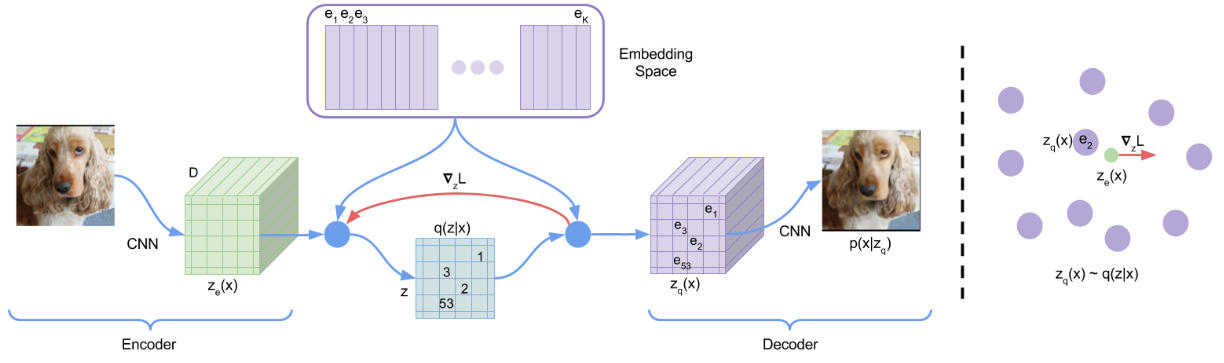
\includegraphics[width=1\textwidth]{images/VQ2.png}
    \caption{VQ-VAE: overall architecture}
    \label{fig:MHA2}
\end{figure}

\subsection{VQ-VAE: Learning}

One can interpret the forward computation pipeline of a VQ-VAE as a standard autoencoder equipped with a peculiar non-linearity that maps the continuous latent vectors into a \textbf{1-of-K} discrete embedding.  
However, this discretization step introduces a major difficulty:  
\textbf{the quantization operation (nearest neighbour lookup) is non-differentiable}.  

Discrete operators such as \texttt{argmax}, \texttt{round} and \texttt{quantize} break the gradient flow during backpropagation.  
To address this issue, VQ-VAE employs a simple but extremely effective technique: the \textbf{Straight-Through Gradient Estimator (STE)}.

\subsubsection{Straight-Through Gradient Estimation}

The key idea behind the STE is to use the discrete code in the forward pass while pretending that the quantization function is the identity during the backward pass.

\begin{itemize}
    \item \textbf{Forward pass:}  
    \[
        z_q = \text{quantize}(z_e)
    \]
    typically via nearest neighbour search in the codebook.
    
    \item \textbf{Backward pass (approximate):}  
    \[
        \frac{\partial L}{\partial z_e} \approx \frac{\partial L}{\partial z_q}
    \]
    The quantization is ignored during backpropagation and treated as the identity function.
\end{itemize}

This trick is widely used beyond VQ-VAEs, for example in:
\begin{compactitemize}
    \item \textbf{Binary neural gates}: forward as a step , backward as a  sigmoid;
    \item \textbf{Neural architecture search} and routing;
    \item \textbf{Pruning and gating mechanisms}.
\end{compactitemize}

\subsection{VQ-VAE: Training Objective}

A critical point is that, due to the straight-through estimator, the embedding vectors $e_i$ in the codebook receive \textbf{no gradient} from the reconstruction loss $\log p(x|z_q(x))$.  
Thus, an additional mechanism is needed to update the codebook.  

VQ-VAE adopts a classical strategy from dictionary learning: \textbf{Vector Quantization}, implemented via simple mean squared error (MSE) terms.

\[
    \mathcal{L} =
    \underbrace{\log p(x|z_q(x))}_{\text{Reconstruction error}}
    +
    \underbrace{\| \text{stopgrad}[z_e(x)] - z_q(x) \|_2^2}_{\text{VQ term}}
    +
    \beta \underbrace{\| z_e(x) - \text{stopgrad}[z_q(x)] \|_2^2}_{\text{Commitment term}}
\]

\paragraph{Interpretation of the three loss components}
\begin{compactitemize}
    \item \textbf{Reconstruction error}  
    Trains only the decoder, encouraging it to reconstruct the input from the selected codeword.

    \item \textbf{Vector Quantization term}  
    Updates the codebook embeddings.  
    It moves each embedding vector $e_k$ closer to the encoder outputs that selected it.

    \item \textbf{Commitment term}  
    Trains the encoder to produce latent vectors $z_e(x)$ that remain close to the chosen codeword.  
    This prevents the encoder from excessively roaming in latent space and promotes stability.
\end{compactitemize}

\paragraph{The stop-gradient operator}
The operator \texttt{stopgrad[$\cdot$]} treats its argument as a constant during backpropagation.  
This allows separating which parts of the loss update the encoder and which parts update the codebook.

\begin{compactitemize}
    \item The \textbf{decoder} optimizes only the reconstruction term.
    \item The \textbf{encoder} optimizes the reconstruction + commitment terms.
    \item The \textbf{embedding space} (codebook) is optimized by the VQ term only.
\end{compactitemize}

This separation is crucial to maintain stable training and prevent collapse of the discrete representations.

\begin{algorithm}[H]
    \caption{VQ-VAE Training Step}
    \textbf{Require:} input $x$, encoder $E(\cdot)$, decoder $D(\cdot)$, codebook $\{e_k\}_{k=1}^K$
    
    $z_e \leftarrow E(x)$ \tcp*[r]{encode input}
    $k \leftarrow \arg\min_j \| z_e - e_j \|_2^2$ \tcp*[r]{nearest codebook entry}
    $z_q \leftarrow e_k$ \tcp*[r]{quantized latent}
    $z_q^{st} \leftarrow z_e + \text{detach}(z_q - z_e)$ \tcp*[r]{Straight-Through Estimator}
    $\hat{x} \leftarrow D(z_q^{st})$ \tcp*[r]{reconstruction}
    
    $L_{\text{rec}} \leftarrow \|x - \hat{x}\|_2^2$ \tcp*[r]{reconstruction loss}
    $L_{\text{codebook}} \leftarrow \|\text{stopgrad}[z_e] - z_q\|_2^2$ \tcp*[r]{VQ term}
    $L_{\text{commit}} \leftarrow \|z_e - \text{stopgrad}[z_q]\|_2^2$ \tcp*[r]{commitment}
    
    $L \leftarrow L_{\text{rec}} + L_{\text{codebook}} + \beta L_{\text{commit}}$ \tcp*[r]{total loss}
    
    \textbf{Backpropagate} and update encoder, decoder, and codebook\;
\end{algorithm}

In the code the implementation if STE is the row:
\[
    z_q^{st}=z_e + detach(z_q - z_e)
\]
Interpretation:
\begin{compactitemize}
    \item Forward: $z_q^{st}=z_q$ (quantization is performed)
    \item Backward: Gradients flow only through $z_e$ (gradient are not affected by quantization)
    \item Effectively treats quantization as the identity function during backpropagation.
\end{compactitemize}

\subsection{VQ-VAE for Image Compression}
VQ-VAE can be used as a learned image compressor:
\begin{compactitemize}
    \item The encoder maps input images to discrete latent codes.
    \item The decoder reconstructs the image from those codes.
    \item The codebook indices can be compressed using entropy coding (e.g., Huffman, arithmetic).
\end{compactitemize}
\begin{figure}[H]
    \centering
    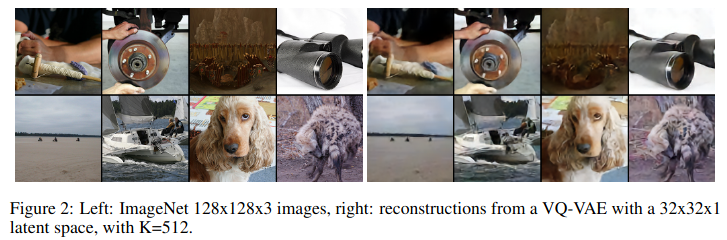
\includegraphics[width=1\textwidth]{images/D3.png}
    \label{fig:MHA2}
\end{figure}
The advantages are:
\begin{compactitemize}
    \item Learn domain-specific features, outperforming handcrafted codecs at low bitrates.
    \item Generates visually coherent reconstructions usin fewer bits.
\end{compactitemize}

\subsection{Learnable Prior in VQ-VAE}
A VQ-VAE learns three main components: an encoder, a decoder, and a codebook of discrete learnable embeddings.  
However, the model does not learn any distribution over the latent codes. This becomes a problem when we want to generate new images.

To synthesize new samples, we would ideally sample vectors from the codebook.  
But if we choose these codes randomly, the resulting images have no meaning: the decoder receives sequences of embeddings that do not correspond to any pattern that occurred in real data.

To fix this, the idea is to \textbf{learn the distribution of the discrete latent codes}.  
In practice:

\begin{compactitemize}
    \item we encode the training images using the VQ-VAE encoder to obtain sequences of codebook indices;
    \item we train a second generative model (e.g., PixelCNN or a Transformer) on these sequences;
    \item this model learns the true distribution over the discrete latent space;
    \item once trained, we can sample new sequences of latent codes from this learned prior;
    \item finally, we pass these sampled codes to the VQ-VAE decoder to generate meaningful new images.
\end{compactitemize}

In this way, the VQ-VAE becomes a complete generative model:  
it not only reconstructs existing inputs, but can also produce new coherent images because sampling occurs from a \textbf{learned prior} rather than from random codebook choices.
\begin{figure}[H]
    \centering
    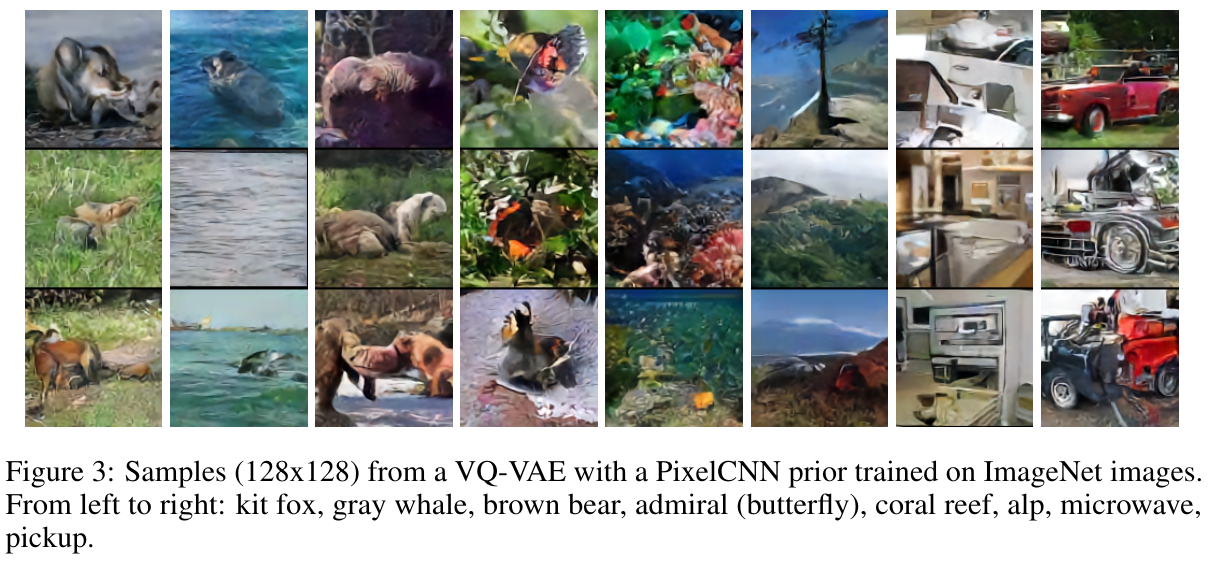
\includegraphics[width=1\textwidth]{images/D4.png}
    \label{fig:MHA2}
\end{figure}

\section{Autoregressive Models (PixelCNN)}
\begin{wrapfigure}{r}{0.3\textwidth}
    \centering
    \vspace{-10pt}
    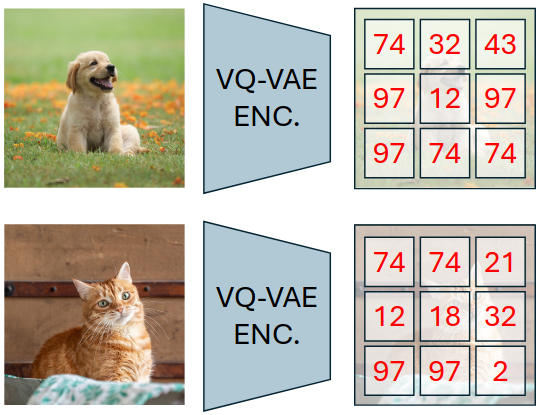
\includegraphics[width=\linewidth]{images/D5.png}
    \label{fig:Scaled Dot Product Attention}
    \vspace{-10pt}
\end{wrapfigure}
With the VQ-VAE model, we have a set of training examples expressed as sequences of \textbf{discrete symbols}:
\[
\{ \mathbf{z}^{(i)} = (z^{(i)}_{1}, z^{(i)}_{2}, \ldots, z^{(i)}_{T}) \}_{i=1}^{N}
\qquad \text{dove } z^{(i)}_{t} \in \{1, \ldots, K\}.
\]

The objective is to learn a generative model (learned prior) on top of these codes, which defines a parametric distribution over sequences of discrete latent variables:
\[
p_{\varepsilon_z}(z), \qquad z = (z_1, z_2, \ldots, z_T), \quad z_t \in \{1, \ldots, K\}.
\]

The main idea is to represent the joint density as a product of conditional distributions, using the chain rule of probability. In particular, the prior \(p_{\varepsilon_z}(z)\) can be learned through an autoregressive factorization of the joint density:
\[
p_{\varepsilon_z}(z) = \prod_{t=1}^{T} p_{\varepsilon_z}(z_t \mid z_{<t}),
\]
where each latent code \(z_t\) is predicted conditioned on all previous codes in the sequence.

To understand this factorization, we start from the definition of conditional probability:
\[
p(A \mid B) = \frac{p(A,B)}{p(B)} \qquad \Longleftrightarrow \qquad p(A,B) = p(A \mid B) \, p(B).
\]

By recursively applying this definition to a sequence of random variables \( z = (z_1, z_2, \ldots, z_T) \), the joint distribution can be decomposed as follows:
\begin{equation}
    \begin{split}
    p(z_1, z_2, \ldots, z_T) 
    &= p(z_T \mid z_1, \ldots, z_{T-1}) \, p(z_1, \ldots, z_{T-1}) \\
    &= p(z_T \mid z_{<T}) \, p(z_1, \ldots, z_{T-1}) \\
    &= p(z_T \mid z_{<T}) \, p(z_{T-1} \mid z_{<T-1}) \, p(z_1, \ldots, z_{T-2}) \\
    &= \cdots \\
    &= p(z_T \mid z_{<T}) \, p(z_{T-1} \mid z_{<T-1}) \, \cdots \, p(z_2 \mid z_1) \, p(z_1) \\
    &= \prod_{t=1}^{T} p(z_t \mid z_{<t}).
    \end{split}
\end{equation}

\begin{wrapfigure}{r}{0.4\textwidth}
    \centering
    \vspace{-10pt}
    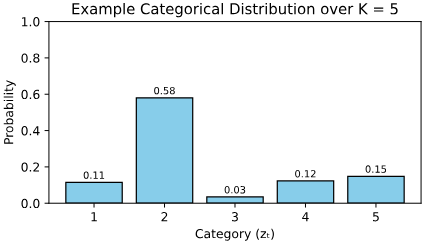
\includegraphics[width=\linewidth]{images/D6.png}
    \label{fig:Scaled Dot Product Attention}
    \vspace{-10pt}
\end{wrapfigure}
In this way, each latent variable is modeled conditioned on the previous ones, allowing the learning of an autoregressive sequential distribution over the discrete codes.

Each latent variable \(z_t\) is a discrete symbol taken from a codebook of size \(K\). In other words, the latent space is categorical, and each \(z_t\) can take one of \(K\) possible values:
\[
z_t \in \{1, \ldots, K\}.
\]

Accordingly, each conditional distribution in the autoregressive factorization can be modeled as a categorical distribution (also called a \emph{multinomial with one trial}):
\[
p_{\varepsilon_z}(z_t \mid z_{<t}) = \mathrm{Cat}(z_t; \pi_{\theta_z}(z_{<t})),
\]
where \(\pi_{\theta_z}(z_{<t})\) represents the vector of probabilities over the \(K\) codebook entries, conditioned on all previous latent variables \(z_{<t} = (z_1, \ldots, z_{t-1})\).  

In this way, the model learns a distribution over the discrete codes at each time step, taking into account the history of the sequence, which allows it to capture sequential dependencies in the latent space.


Each conditional distribution in the autoregressive factorization can be modeled as a categorical distribution:
\[
p_{\theta_z}(z_t \mid z_{<t}) = \mathrm{Cat}(z_t; \pi{\theta}(z_{<t})), \qquad z_t \in \{1, \ldots, K\},
\]
where \(\pi_{\theta}(z_{<t}) \in \mathbb{R}^{K \times 1}\) is the predicted probability vector over the \(K\) codebook entries. This vector can be parametrized by a neural network, which allows the model to flexibly learn how the probability of each code depends on the previous latent variables.  

Common choices for modeling \(p_{\theta_z}\) include:

\begin{compactitemize}
    \item \textbf{Pixel Recurrent Neural Networks (PixelRNN)}: uses recurrent connections over the sequence, less common for image latents.
    \item \textbf{PixelCNN}: a convolutional approach that is aware of the spatial grid structure, often used for image-based latents.
    \item \textbf{Transformer}: uses flexible attention-based mechanisms to model dependencies over the entire sequence, providing powerful context modeling.
\end{compactitemize}

In summary, by parameterizing each conditional as a neural network-predicted categorical distribution, the autoregressive model can capture complex sequential dependencies in the discrete latent space, allowing for rich generative modeling.

\subsection{PixelCNN: Inference}
The general idea is to model the prior over discrete latent variables 
\[
z \in \{1, \dots, K\}^{H \times W}
\] 
using a 2D autoregressive model. This is typically implemented via a (modified) Convolutional Neural Network (CNN), such as a PixelCNN.  

The joint distribution of the latents is factorized in raster scan order (row by row, left to right):
\[
p_{\theta_z}(z) = \prod_{i=1}^{H} \prod_{j=1}^{W} p_{\theta_Z}(z_{i,j} \mid z_{<i,j}),
\]
where \(z_{<i,j}\) denotes all previously generated pixels (or latent variables) in the raster scan order.  


Each conditional distribution 
\[
p_{\theta_z}(z_{i,j} \mid z_{<i,j})
\] 
is modeled as a categorical distribution whose probabilities are predicted by a convolutional neural network with \emph{masking} (\textbf{causal convolutions}), ensuring that no future pixel information is used when predicting the current pixel.

\[
p_{\theta_z}(z_{i,j} \mid z_{<i,j}) = \mathrm{Cat}(z_{i,j}; \pi_{\theta_z}(z_{<i,j})), 
\quad \pi_{\theta_z}(z_{<i,j}) = \mathrm{PixelCNN}(z_{<i,j}; \theta_z)
\]

\textbf{Inference (Sampling).}  
Sampling is performed sequentially following the raster scan order:

\begin{enumerate}
    \item Start with an empty image or latent grid.  
    \item For each pixel or latent variable \((i,j)\):
    \begin{enumerate}
        \item Perform a forward pass through the PixelCNN to obtain the conditional distribution \(\pi_{\theta_z}(z_{<i,j})\).  
        \item Sample \(z_{i,j}\) from the predicted categorical distribution:
        \[
        z_{i,j} \sim p_{\theta_z}(z_{i,j} \mid z_{<i,j}).
        \]  
        \item Fill in the grid sequentially, one pixel at a time.
    \end{enumerate}
\end{enumerate}

This approach allows the model to capture complex spatial dependencies among the latent variables, while maintaining a fully probabilistic generative model over the 2D latent grid.

\subsection{PixelCNN: Sampling}
At generation time, pixel are sampled one by one, in raster-scan order (left-to-right, top-to-bottom), using the predicted distribution conditioned on previous generated pixel.

This proccess is inherently \textbf{slow}, as each pixel depends on all previous one, but this ensueres valide sample frome the model.

This proccess lead at the fact that this infernce cannot be parallelized and the sampling time scales linearly with the number of pixel.

\subsection{Causal Convolutions}

In autoregressive models, such as PixelCNN, it is crucial to ensure that the prediction at position \((i,j)\) only depends on previously generated positions. This is necessary to avoid \textbf{information leakage}, i.e., the network accidentally using information from pixels it is supposed to predict.  

\begin{wrapfigure}{r}{0.14\textwidth}
    \centering
    \vspace{-10pt}
    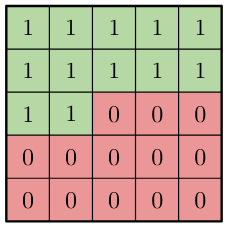
\includegraphics[width=\linewidth]{images/D7.png}
    \label{fig:Scaled Dot Product Attention}
    \vspace{-10pt}
\end{wrapfigure}
To enforce this constraint, PixelCNN uses \textbf{masked convolutions}. The basic idea is to prevent the convolutional kernel from “seeing” future pixels. This is typically implemented by \textbf{element-wise multiplying the convolutional kernel with a binary mask} before each forward pass. Such a mask is usually \textbf{hard-coded}, meaning that the positions that can be accessed are predefined and fixed, not learned by the network.  

\begin{infobox}[Hard-coded Binary Mask]
A \textbf{hard-coded binary mask} is a matrix of 0s and 1s that is multiplied element-wise with the convolutional kernel. 

- \textbf{1} indicates that the position is allowed to contribute to the output (can be “seen” by the convolution).  
- \textbf{0} indicates that the position is blocked (cannot be used).  

In a 2D autoregressive setting, this ensures that the convolution only attends to past pixels (above and to the left), enforcing the autoregressive constraint.
\end{infobox}

For 2D data such as images, PixelCNN typically uses two types of masks:

\begin{compactitemize}
    \item \textbf{Mask type A}: excludes the current pixel \((i,j)\). This is used in the \textbf{first layer} only, to enforce strict causality and prevent the network from seeing the pixel it is trying to predict.  
    \item \textbf{Mask type B}: includes the current pixel \((i,j)\). This is used in \textbf{all subsequent layers}, allowing the network to incorporate richer context from the feature maps of previous layers while still respecting the autoregressive property.  
\end{compactitemize}

\begin{infobox}[Why this distinction?]
- Type A is necessary in the \textbf{first layer} because at that stage the network has not yet seen any features derived from the current pixel, so strict causality must be enforced.  
- Type B is used in deeper layers because the original pixel at \((i,j)\) was never observed in the first layer, so allowing access to this position in the feature maps does not violate the autoregressive property. Instead, it provides \textbf{richer context} to the network, improving its ability to model complex dependencies.
\end{infobox}

\subsection{PixelCNN: Training}
During training, \textbf{PixelCNN suffers from slow sampling}, since its autoregressive structure requires the model to generate each pixel sequentially. For every pixel location, the model must perform a forward pass conditioned on all previously generated pixels. This strict dependency makes sampling extremely slow, especially for high-resolution images.

To address this issue, we use \textbf{Teacher Forcing}, which becomes feasible during training because \textbf{ground-truth pixel values (or latent codes) are available}. Instead of allowing the model to generate one pixel at a time and feeding its own predictions back as inputs, Teacher Forcing provides the true pixel values at each location as conditioning information. As a result, \textbf{the model does not rely on its own predictions during training}, eliminating the need for sequential generation.
\begin{wrapfigure}{r}{0.6\textwidth}
    \centering
    \vspace{-10pt}
    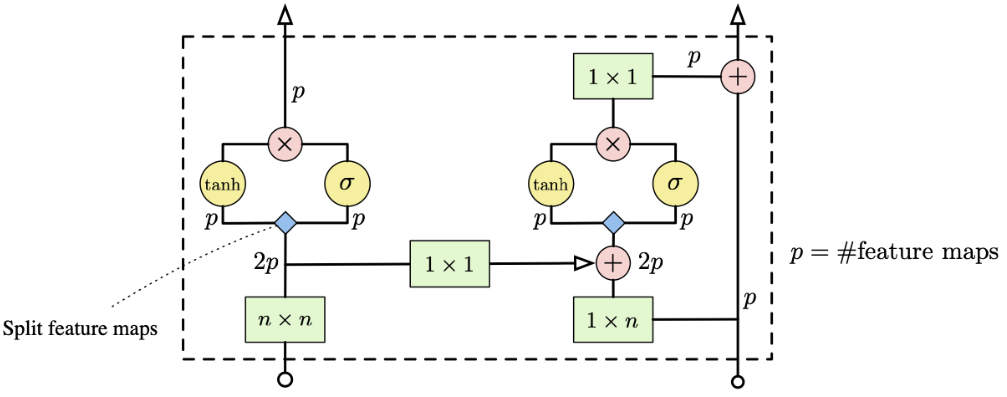
\includegraphics[width=\linewidth]{images/D9.png}
    \label{fig:Scaled Dot Product Attention}
    \vspace{-10pt}
\end{wrapfigure}
With Teacher Forcing, \textbf{PixelCNN can predict all pixels in parallel through a single forward pass}, since each prediction is conditioned on the ground-truth values rather than sampled outputs. This makes training highly efficient: \textbf{no autoregressive sampling loop is required}, and the entire image can be processed simultaneously. Consequently, even though PixelCNN still requires sequential sampling during inference, \textbf{training becomes fully parallelizable and drastically faster}, enabling practical optimization of autoregressive models despite slow sampling at inference time.
\begin{figure}[H]
    \centering
    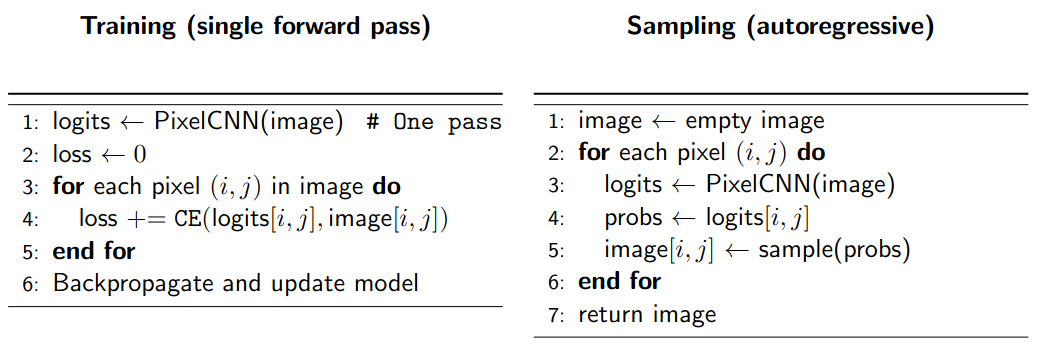
\includegraphics[width=1\textwidth]{images/D8.png}
    \label{fig:MHA2}
\end{figure}

\subsection{PixelCNN: Likelyhood and Anomaly Detection}
PixelCNN models the exact data likelihood using an autoregressive factorization of the image distribution:

\[
\log p(x) = \sum_{i,j} \log p(x_{i,j} \mid x_{<i,j})
\]

This likelihood can be computed efficiently in a single forward pass by using masked convolutions, which ensure that each pixel prediction depends only on the valid preceding pixels. As a result, PixelCNN allows us to assign a probability score (or log-likelihood) to any image directly.

This capability enables several important applications. One key use case is \textbf{anomaly detection}, where unusual or corrupted images typically exhibit very low likelihood under the model. Another closely related application is \textbf{novelty detection}, in which out-of-distribution (OOD) samples can be identified by thresholding their likelihood scores. High-likelihood images are considered consistent with the training distribution, while low-likelihood ones are flagged as novel or anomalous.

\subsection{Summary}
\textbf{VQ-VAE: Vector Quantized Variational Autoencoder:} 
Learns a \textbf{discrete latent space} through vector quantization. The encoder maps inputs to discrete latent codes using a learned codebook, while the decoder reconstructs the original input from these codes. This framework enables \textbf{efficient and compressible representations} by replacing continuous latent variables with discrete embeddings.

\textbf{PixelCNN:} 
PixelCNN models the \textbf{joint distribution over the discrete latent codes} produced by the VQ-VAE encoder. It is trained directly on these latents to learn a powerful generative prior. Once trained, PixelCNN can sample new latent code grids, which are then passed to the VQ-VAE decoder to generate images.

\textbf{Combined Pipeline:} 
The overall system works in two stages:  
\begin{compactitemize}
    \item \textbf{Train the VQ-VAE} to learn a discrete latent representation and a decoder capable of reconstructing images from latent codes.
    \item \textbf{Train PixelCNN on the discrete latent maps} to model their distribution and serve as a generative prior.    
\end{compactitemize}

At generation time, samples are drawn from the PixelCNN prior and subsequently decoded using the VQ-VAE decoder, producing fully generated images.

\section{Gumbel-Softmax}
\begin{wrapfigure}{r}{0.3\textwidth}
    \centering
    \vspace{-10pt}
    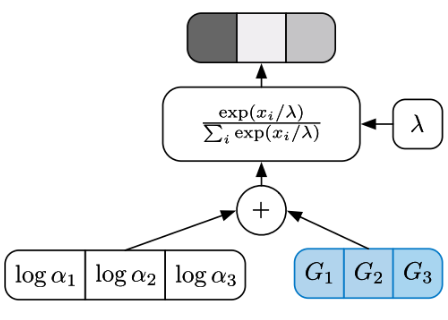
\includegraphics[width=\linewidth]{images/D10.png}
    \label{fig:Scaled Dot Product Attention}
    \vspace{-10pt}
\end{wrapfigure}
As we saw in the first example of this chapter, the \textbf{argmax} function is not differentiable and therefore breaks the training process. We also discussed a workaround known as the \textbf{Straight-Through Estimator (STE)}, which consists of performing the discrete sampling during the forward pass while treating the operation as the identity function during the backward pass in order to propagate gradients.

However, there exists another approach to avoid the non-differentiability of the argmax: the \textbf{Gumbel-Softmax} trick. This method allows us to sample from a categorical distribution during the forward pass of a neural network while still maintaining differentiability with respect to the logits.

In this setting, the encoder produces logits over the codebook entries. Instead of selecting a single discrete index, we sample a \emph{soft} categorical vector using the Gumbel-Softmax formulation:

\[
y_k = \frac{\exp\left( \frac{\log \pi_k + g_k}{\lambda} \right)}
{\sum_{j} \exp\left( \frac{\log \pi_j + g_j}{\lambda} \right)}
\]

where:
\begin{compactitemize}
    \item $\pi_k$ are the unnormalized probabilities (logits) of the categorical distribution,
    \item $g_k$ are i.i.d.\ Gumbel noise samples,
    \item $\lambda$ is the temperature parameter controlling the softness of the distribution.
\end{compactitemize}

As $\lambda \to 0$, the distribution becomes increasingly sharp and approximates a one-hot categorical sample. For higher values of $\lambda$, the output is smoother and fully differentiable. This mechanism shares strong similarities with the \textbf{Reparameterization Trick} used in continuous VAEs, as it enables gradient-based optimization through a stochastic sampling step. The Gumbel-Softmax therefore provides a principled and differentiable alternative to the STE for learning discrete latent representations.
\begin{figure}[H]
    \centering
    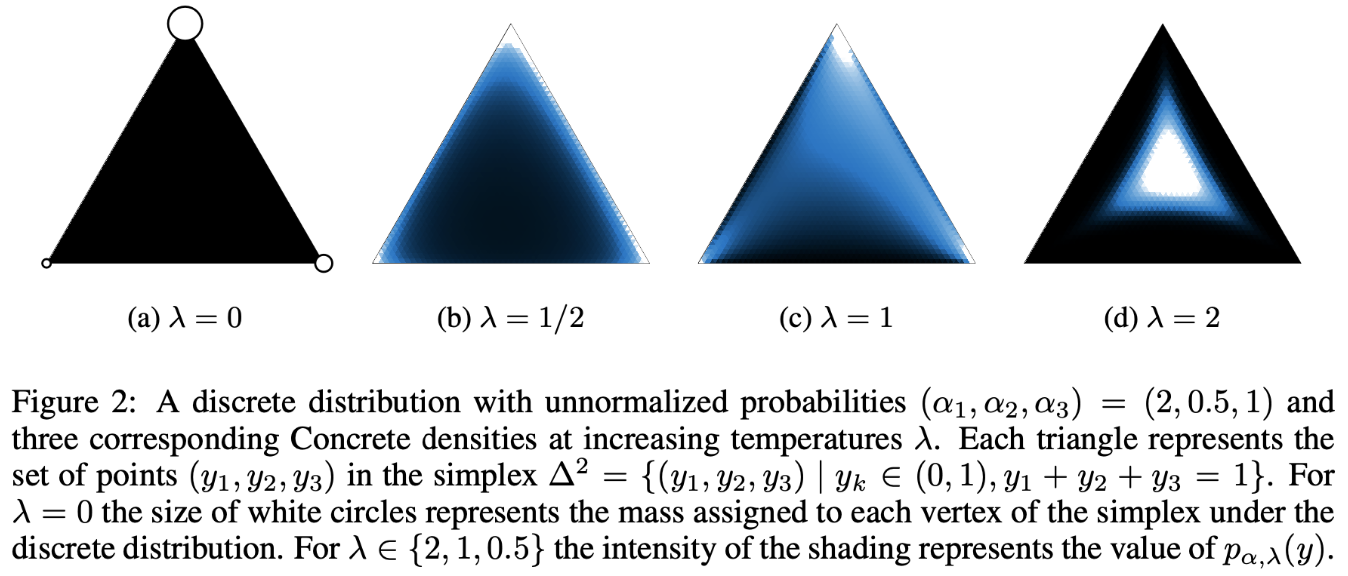
\includegraphics[width=1\textwidth]{images/D11.png}
    \label{fig:MHA2}
\end{figure}

\begin{figure}[H]
    \centering
    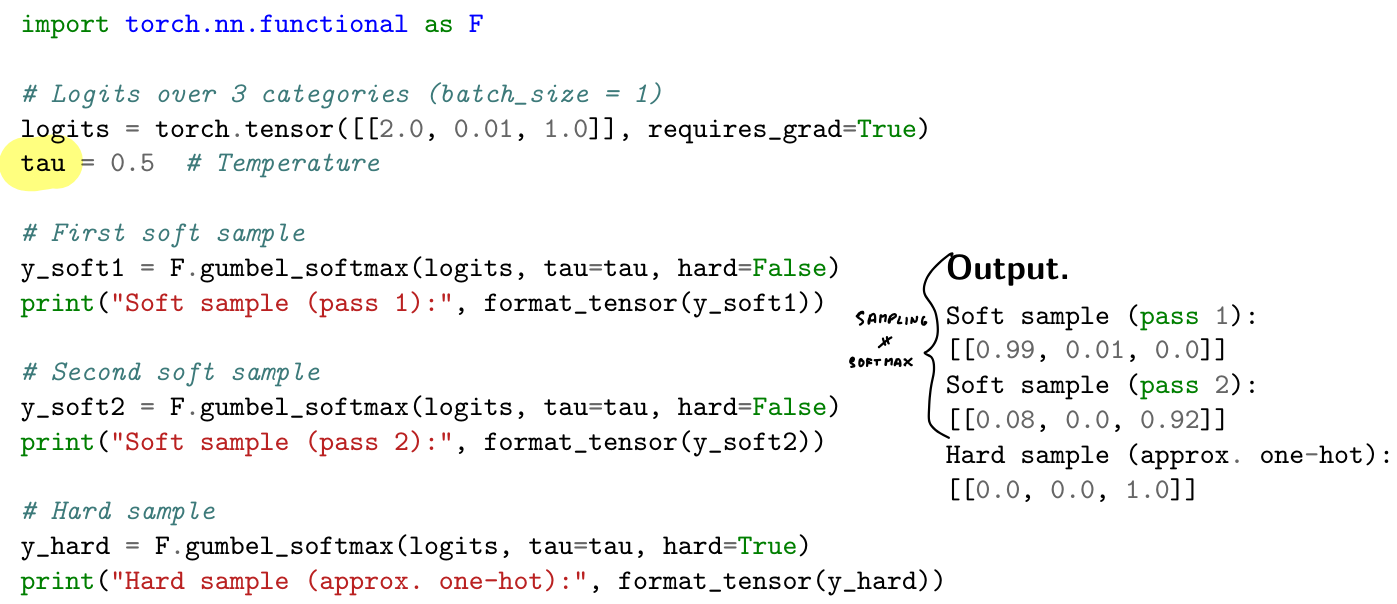
\includegraphics[width=1\textwidth]{images/D12.png}
    \label{fig:MHA2}
\end{figure}
\begin{infobox}[Sampling vs Softmax]
    When using the standard \textbf{softmax} function on the logits produced by the encoder, the output is \emph{deterministic}.  
    Given the same input $x$, the encoder always produces the same logits, and the softmax always produces the same probability vector.  
    This is useful for classification, but it does \emph{not} allow us to sample discrete latent variables.

    In contrast, the \textbf{Gumbel-Softmax} introduces \emph{stochasticity} by adding Gumbel noise to the logits before applying a temperature-controlled softmax.  
    This means that even if the encoder outputs the same logits at every forward pass, the addition of random Gumbel noise causes the resulting Gumbel-Softmax vector to be \textbf{different each time}.  
    Thus, the model can produce \emph{different samples} from the same categorical distribution.

    This is the key advantage:  
    \begin{compactitemize}
        \item We want to \textbf{sample} a discrete latent variable (like choosing a codebook entry).  
        \item But we also want the entire operation to remain \textbf{differentiable}, so gradients can pass through the sampling step.
    \end{compactitemize}

    The Gumbel-Softmax bridges this gap:
    \begin{compactitemize}
        \item It behaves like sampling because the Gumbel noise randomizes the output.  
        \item It remains differentiable because the output after applying the temperature softmax is still a continuous vector.
    \end{compactitemize}
\end{infobox}
\begin{figure}[H]
    \centering
    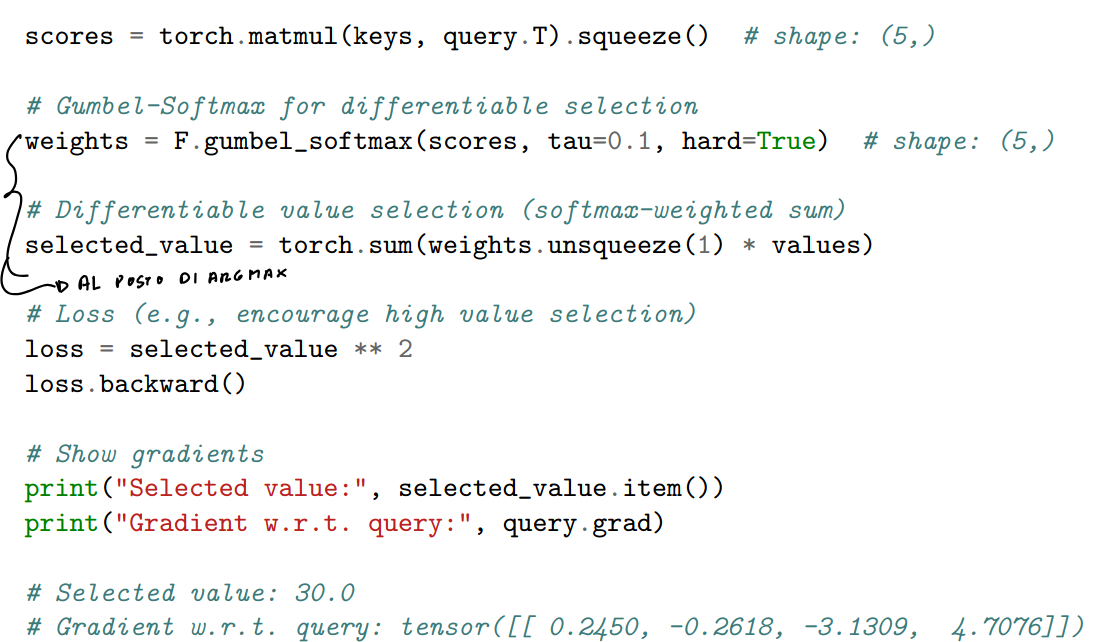
\includegraphics[width=1\textwidth]{images/D13.png}
    \caption{The initial example: Now}
    \label{fig:MHA2}
\end{figure}
\chapter{Uncertainty Estimation and Calibration in Deep Neural Networks}

Deep Neural Networks (DNNs) have shown remarkable success in a wide range of fields. 
Although they have become increasingly appealing for high-risk domains such as medical image analysis 
or autonomous vehicle control, their deployment in \textbf{safety-critical} real-world applications 
remains limited.

This is because, in such contexts, we not only require the model to be accurate, but we also need to 
understand when the model is likely to be incorrect. For example, suppose we have a model that outputs 
the probability that a patient is affected by a brain tumor. Along with the prediction, the network 
also provides a value representing the reliability of that prediction. If this confidence value falls 
below a specified threshold, the prediction is discarded and a human expert is consulted instead.

The NNs are affected by several issues that lead to \textbf{uncertainty}. These problems are:
\begin{compactitemize}

    \item \textbf{Lack of Transparency}.  
    DNNs typically behave as \emph{black-box} models, meaning that their internal decision-making process is not easily interpretable by humans. This lack of transparency makes it difficult to understand why a model produces a certain output and prevents users from meaningfully assessing how confident the model is in its predictions.

    \item \textbf{Overconfident Predictions}.  
    Although neural networks output a distribution \(p(y \mid x, \theta)\) intended to represent class probabilities, they are often excessively confident even when their predictions are wrong. Model confidence is commonly inferred from the maximum softmax probability, but the softmax function is not a reliable measure of uncertainty: it can produce arbitrarily high values even for inputs that lie far outside the training distribution. Essentially, this problem occurs when the network assigns a score close to 1 to the predicted class; with such artificially high confidence, it becomes difficult to correctly estimate the true uncertainty.

    \item \textbf{Out-of-Distribution (OOD) Sensitivity}.  
    Due to their tendency toward overconfidence, DNNs often fail to distinguish between in-domain and out-of-domain samples. As a result, users or downstream systems may trust predictions that are actually meaningless or invalid. In high-risk contexts such as medical diagnosis or autonomous driving, this inability to detect OOD inputs can lead to dangerous failures without any warning signal.
    Due to this, we want that our model must recognize input that not belong to the original distribution.
    \item \textbf{Adversarial Vulnerability}.  
    Deep neural networks are sensitive to adversarial attacks—small, carefully crafted perturbations that are imperceptible to humans but cause the model to produce incorrect or unexpected outputs with high confidence. This vulnerability highlights fundamental weaknesses in the model’s robustness and further complicates the reliable estimation of uncertainty.
\end{compactitemize}
\begin{figure}[H]
    \centering
    \begin{minipage}{0.4\textwidth}
        \centering
        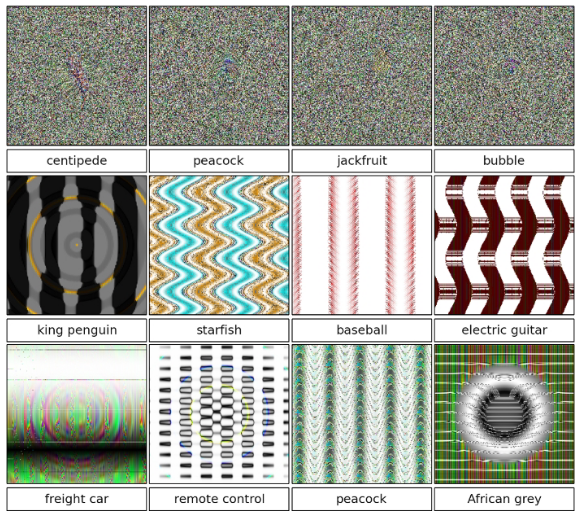
\includegraphics[width=\textwidth]{images/U2.png}
        \caption{OOD detection}
        \label{fig:Residuals}
    \end{minipage}
    \label{fig:TS_Residuals}
    \hfill
    \begin{minipage}{0.55\textwidth}
        \centering
        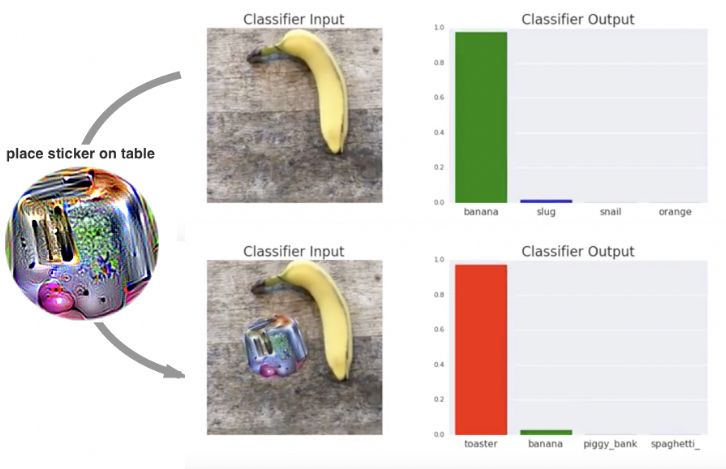
\includegraphics[width=\textwidth]{images/U3.png}
        \caption{Adversarial Attacks}
        \label{fig:Residuals}
    \end{minipage}
    \label{fig:TS_Residuals}
\end{figure}

To overcome these limitations and ensure safe decision-making in high-risk fields – including domains such as medical diagnosis, autonomous systems, and business intelligence – it is essential to provide \textbf{uncertainty estimates}, such that some predictions can be ignored or passed to human experts.

There are two different types of uncertainty. Let's see them:
\begin{compactitemize}

    \item \textbf{Aleatoric Uncertainty} (data uncertainty): arises from inherent noise, ambiguity, or class overlap in the data. It \textbf{persists regardless of how much data is collected}, as it is caused by randomness inherent in the data-generating process. This type of uncertainty \textbf{cannot be eliminated} even with more observations. It captures variability due to \textbf{measurement noise}, \textbf{ambiguous inputs}, or \textbf{naturally stochastic phenomena}. Aleatoric uncertainty occurs, for example, when the same input can correspond to multiple valid outputs, making the prediction task fundamentally ambiguous (e.g., label noise, sensor imprecision, or overlapping classes).  
    One example of this type of uncertainty is \textbf{stock price movement}: even if we were able to observe all relevant variables and theoretically make an accurate prediction, the data still contains inherent noise that makes the price evolution unpredictable.

    \item \textbf{Epistemic Uncertainty} (model uncertainty or systematic uncertainty): arises from a \textbf{lack of knowledge} about the underlying data distribution or model parameters. It is due to factors that one could, in principle, know but does not in practice. This uncertainty reflects the model’s \textbf{ignorance about the data}, often caused by limited, biased, or incomplete training sets. It captures uncertainty in the model’s parameters, structure, or ability to generalize to unseen data. Epistemic uncertainty also emerges when the model encounters unfamiliar situations that lie far from the training distribution. Unlike aleatoric uncertainty, \textbf{epistemic uncertainty can be reduced} by collecting more data or using better, more expressive models.

\end{compactitemize}

\section{Methods for Uncertainty Quantification}

\subsection{Deep Ensembles}
Deep Ensembles are one of the simplest and most effective approaches for uncertainty quantification in deep neural networks. The idea is to train multiple independent neural networks, each initialized with different random seeds and exposed to different shufflings of the training data. Because of this randomness, each model converges to a different local minimum, yet all solutions remain consistent with the data. The degree to which these models agree or disagree provides a natural estimate of \textbf{epistemic uncertainty}: if all models produce similar predictions, confidence is high; if they diverge, uncertainty increases.

\begin{wrapfigure}{r}{0.4\textwidth}
    \centering
    \vspace{-10pt}
    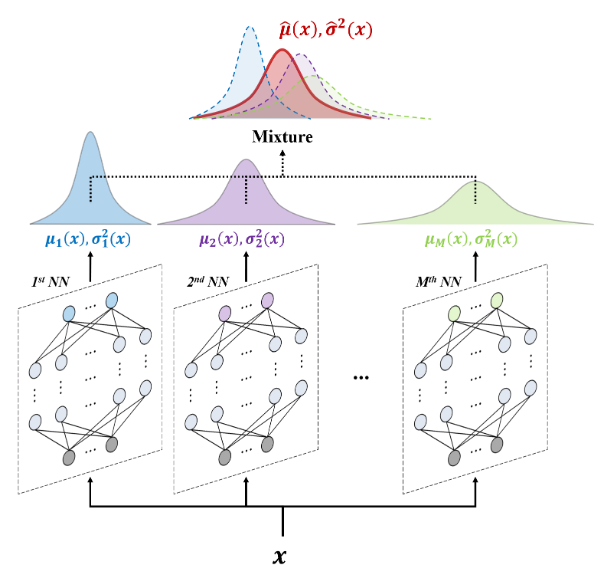
\includegraphics[width=\linewidth]{images/U4.png}
    \label{fig:Scaled Dot Product Attention}
    \vspace{-10pt}
\end{wrapfigure}
More precisely, when networks operate in regions of the input space that are well covered by training samples, they tend to produce similar outputs. However, in data-scarce regions, their predictions diverge, and this disagreement becomes a strong indicator of model uncertainty. Beyond simple ensembling, several tricks exist for improving uncertainty estimation, especially in regression tasks or robustness-oriented training paradigms.

\subsubsection{Predictive Uncertainty in Regression.}  
In standard regression settings, neural networks are typically trained to predict only the mean value $\mu(x)$ of the target variable, optimized through the Mean Squared Error (MSE) objective:
\[
\sum_{n=1}^{N} (y_n - \mu(x_n))^2.
\]
This formulation, however, does not capture any form of uncertainty, as it provides point estimates only. A more suitable approach is to predict both the mean $\mu(x)$ and the variance $\sigma^2(x) > 0$. Assuming a Gaussian likelihood
\[
y \sim \mathcal{N}(\mu(x), \sigma^2(x)),
\]
the model can be trained by minimizing the Negative Log-Likelihood (NLL):
\[
- \log p(y_n \mid x_n) = \log \sigma^2(x) + \frac{(y_n - \mu(x))^2}{\sigma^2(x)} + \text{const}.
\]
In practice, the variance is often constrained to be positive using a softplus activation or by adding a small constant (e.g., \(10^{-6}\)) for numerical stability.

\subsubsection{Merging Predictions in Ensembles (Classification).}  
Once the $M$ ensemble models have been trained, their predictions must be combined into a single predictive distribution. For classification, the ensemble is treated as a uniformly weighted mixture of models. The final predictive distribution is simply the average of the individual softmax probabilities:
\[
p_{E}(y \mid x) = \frac{1}{M} \sum_{m=1}^{M} p_{\theta_m}(y \mid x).
\]
To quantify model disagreement (epistemic uncertainty), one can compute the sum of Kullback–Leibler divergences between each model and the ensemble distribution:
\[
\sum_{m=1}^{M} \mathrm{KL}\big( p_{\theta_m}(y \mid x) \,\|\, p_{E}(y \mid x) \big).
\]

\subsubsection{Merging Predictions in Ensembles (Regression).}  
For regression tasks, each model in the ensemble outputs a predicted mean and variance, namely $\mu_m(x)$ and $\sigma_m^2(x)$ for $m = 1, \dots, M$. The ensemble prediction can be interpreted as a uniform mixture of $M$ Gaussian distributions. This mixture is often approximated by a single Gaussian with mean and variance given by:
\[
\mu_{\text{ens}}(x) = \frac{1}{M} \sum_{m=1}^{M} \mu_m(x),
\]
\[
\sigma_{\text{ens}}^{2}(x) 
= 
\frac{1}{M} \sum_{m=1}^{M} \left( \sigma_m^{2}(x) + \mu_m^{2}(x) \right) - \mu_{\text{ens}}^{2}(x)
=
\underbrace{
\frac{1}{M} \sum_{m=1}^{M} \sigma_m^{2}(x)
}_{\text{Aleatoric uncertainty}}
\;+\;
\underbrace{
\left[
\frac{1}{M} \sum_{m=1}^{M} \mu_m^{2}(x)
- \mu_{\text{ens}}^{2}(x)
\right]
}_{\text{Epistemic uncertainty}}.
\]
The resulting predictive variance includes both aleatoric and epistemic components, naturally decomposed through the ensemble formulation.

\subsubsection{Additional Technique: Adversarial Training.}  
Deep neural networks are known to be vulnerable to adversarial examples—small perturbations to the input that cause the model to produce incorrect but highly confident predictions. Adversarial training improves model robustness and often leads to smoother and more reliable predictive distributions.

The idea is to expose each ensemble model to adversarially perturbed inputs during training. A common approach is to generate adversarial samples using the Fast Gradient Sign Method (FGSM):
\[
x_{\text{adv}} = x + \epsilon \cdot \mathrm{sign}(\nabla_x L(x, y)),
\]
where $\epsilon$ controls the strength of the perturbation. The model is then trained on both clean and adversarial examples via the objective:
\[
\min_{\theta} \; \mathbb{E}_{(x, y)} \left[ L(f_{\theta}(x), y) \;+\; \lambda \cdot L(f_{\theta}(x_{\text{adv}}), y) \right],
\]
where $\lambda$ balances standard and adversarial training.  
When applied within an ensemble, adversarial training encourages each model to learn smoother decision boundaries, ultimately leading to more stable and calibrated uncertainty estimates.

\subsubsection{Limitations of Deep Ensembles}

Deep Ensembles are simple, empirically strong, and widely adopted for uncertainty quantification. 
However, despite their effectiveness, they also present several important limitations that motivate 
the search for more principled Bayesian approaches. The principal limitations are:
\begin{compactitemize}
    \item \textbf{High computational cost }: Deep Ensembles require training multiple independent neural networks from scratch, each with different random initializations and data shuffling. This leads to a computational overhead that grows linearly with the ensemble size. Memory usage also increases proportionally, making the method less suitable for large models or resource-constrained devices. Inference is slower as well, since it requires multiple forward passes—one for each ensemble member.

    \item \textbf{Limited diversity among ensemble members}: Although ensembles rely on model diversity to estimate epistemic uncertainty, in practice the members may converge to similar solutions, especially when trained on large datasets. As a consequence, the ensemble may underestimate epistemic uncertainty due to insufficient variability among the models.
\end{compactitemize}

Deep Ensembles show that averaging predictions of many diverse models improves uncertainty estimation. A natural question then arises: \emph{what if we could average not just a handful of models, but infinitely many?}  
One might consider generating an unbounded number of networks with random parameters and averaging their predictions. However, most randomly generated networks would produce meaningless outputs, yielding a poor approximation of meaningful uncertainty.

\subsubsection{Bayesian solution: weighted model averaging.}  
Instead of averaging arbitrary models, a Bayesian approach assigns higher probability to models whose parameters are more plausible given the dataset. Formally, the predictive distribution is defined as:
\[
p(y \mid x, D) = \int p(y \mid x, w) \, p(w \mid D) \, dw,
\]
where:
\begin{compactitemize}
    \item \(w\) are the model parameters,
    \item \(p(w \mid D)\) is the posterior distribution over parameters given the dataset \(D\),
    \item \(p(y \mid x, w)\) is the model likelihood,
    \item \(p(y \mid x, D)\) is the \emph{posterior predictive distribution} obtained by marginalizing over all plausible models.
\end{compactitemize}

Computing this integral exactly is intractable for modern neural networks. Therefore, Bayesian methods approximate it using \textbf{Monte Carlo} integration:
\[
p(y \mid x, D) \approx \frac{1}{J} \sum_{j=1}^{J} p(y \mid x, w_j), 
\qquad w_j \sim p(w \mid D).
\]

Two main families of methods are used to approximate samples from the posterior:
\begin{compactitemize}
    \item \textbf{Sampling-based methods}, such as Markov Chain Monte Carlo (MCMC).
    \item \textbf{Deterministic approximations}, such as Laplace approximations and Variational Inference.
\end{compactitemize}

\begin{infobox}[Connection to Deep Ensembles]
    Deep Ensembles can be interpreted as approximating the posterior \(p(w \mid D)\) with a set of 
    point masses located at different modes of the loss landscape. Although this is a crude approximation, 
    it is surprisingly effective in practice.
\end{infobox}

\subsubsection{Variational Inference (VI).}  
A popular deterministic Bayesian approach is Variational Inference. The idea is to approximate the true posterior \(p(w \mid D)\) with a simpler, tractable distribution \textbf{\(q_{\theta}(w)\)}, typically chosen within a parametric family (e.g., a Gaussian). The procedure is:
\begin{enumerate}
    \item Choose a family of approximate distributions \(q_{\theta}(w)\).
    \item Find the member \(q_{\theta}(w)\) that is closest to the true posterior by minimizing:
    \[
    \mathrm{KL}\big(q_{\theta}(w) \,\|\, p(w \mid D)\big).
    \]
    \item Once learned, samples \(w_j \sim q_{\theta}(w)\) can be drawn to approximate the predictive distribution:
    \[
    p(y \mid x, D) \approx \frac{1}{J} \sum_{j=1}^{J} p(y \mid x, w_j).
    \]
\end{enumerate}

Variational Inference can be seen as “turning integration into optimization,” making Bayesian model averaging computationally feasible while capturing epistemic uncertainty more rigorously than Deep Ensembles alone.

\subsection{Bayesian Neural Network (BNN)}
\begin{wrapfigure}{r}{0.6\textwidth}
    \centering
    \vspace{-10pt}
    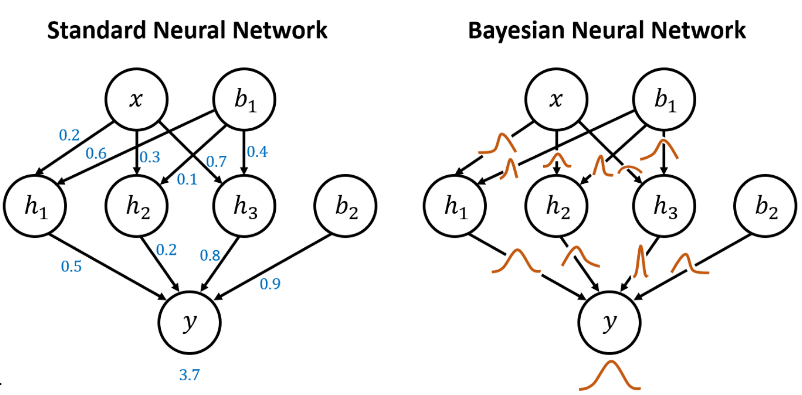
\includegraphics[width=\linewidth]{images/U5.png}
    \label{fig:Scaled Dot Product Attention}
    \vspace{-10pt}
\end{wrapfigure}

The approximate weight distribution $q_\theta(w) \approx p(w \mid D)$, introduced in the previous subsection, can be implemented through a \textbf{Bayesian Neural Network} (BNN). Unlike standard neural networks, which treat each parameter as a fixed value, BNNs represent every weight through a probability distribution. This leads to fundamental conceptual and practical differences between the two approaches.

\textbf{Standard Neural Networks}: In traditional neural networks, parameters are represented by single \emph{point estimates}. Training finds a specific set of weights $w^\ast$ that minimizes a given loss function. Because weights are fixed values, uncertainty is not explicitly modeled; the network produces deterministic outputs, and any regularization (e.g., weight decay, dropout) must be manually injected during training. As a consequence, these models cannot naturally quantify epistemic uncertainty and often rely on ensemble strategies to obtain more reliable predictions.

\textbf{Bayesian Neural Networks}: In BNNs, each weight is characterized by a probability distribution rather than a single value. Training starts by introducing a prior distribution $p(w)$ and updating it to a posterior $p(w \mid D)$ through Bayesian learning. This turns the model parameters into random variables and allows the BNN to explicitly capture \textbf{epistemic uncertainty}. Regularization arises naturally from the prior, reducing the need for manual techniques.  

Representing each weight through a distribution typically requires storing \emph{two} values—commonly a mean and a variance—doubling the memory footprint compared to standard networks. Despite this cost, BNNs offer an important advantage: because the model is \textbf{stochastic}, a single BNN can produce multiple plausible predictions by sampling different weight configurations from $q_\theta(w)$. This means that, unlike Deep Ensembles, we do not need to train many distinct deterministic networks; one stochastic model is sufficient to approximate Bayesian model averaging. Consequently, BNNs provide a theoretically grounded and memory-efficient alternative to ensembles for uncertainty estimation, particularly when combined with Variational Inference to approximate the intractable posterior distribution.

\begin{infobox}[Which are the most important weights?]
    The most important weights in the network are those with very small variance.
    This is intuitive: parameters with high variance do not significantly influence the output, since their value can fluctuate without affecting the prediction. 
    In contrast, parameters whose distribution is tightly concentrated around the mean are crucial for the model, as their value has a meaningful impact on the output.
\end{infobox}


\subsection{Bayes by BackPropagation}
\begin{wrapfigure}{r}{0.4\textwidth}
    \centering
    \vspace{-10pt}
    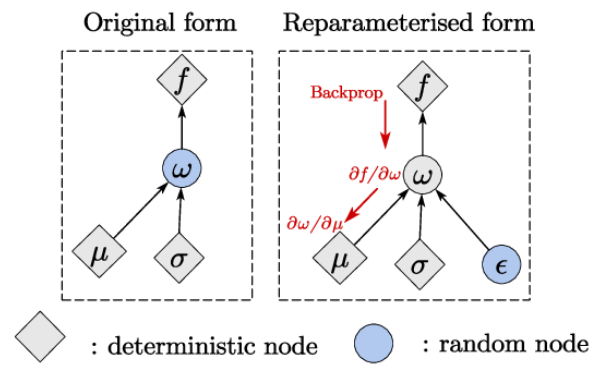
\includegraphics[width=\linewidth]{images/U6.png}
    \label{fig:Scaled Dot Product Attention}
    \vspace{-10pt}
\end{wrapfigure}
Bayes by Backprop  is one of the foundational methods for training Bayesian Neural Networks using variational inference combined with standard backpropagation. The key idea is to learn an approximate posterior distribution over the network weights instead of point estimates, enabling principled epistemic uncertainty estimation.

The method starts by introducing a prior distribution over the weights, typically chosen as an isotropic Gaussian:
\[
p(w) = \mathcal{N}(w \mid 0, \alpha^{-1} I),
\]
where $\alpha$ denotes the precision (i.e., the inverse variance).  
The variational posterior is modeled as another Gaussian distribution,
\[
q_\theta(w) = \mathcal{N}(w \mid \mu, \sigma^2),
\]
whose parameters $(\mu, \sigma)$ are learned during training. The training objective is to minimize the negative Evidence Lower Bound (ELBO):
\[
\mathcal{L}(\theta) = \mathrm{KL}(q_\theta(w) \,\|\, p(w)) - 
\mathbb{E}_{q_\theta(w)}[\log p(D \mid w)],
\]
which trades off model complexity (the KL term) and data fit (the likelihood term).

To make the optimization tractable, Bayes by Backprop uses the \textbf{reparameterization trick}. Instead of sampling $w$ directly from $q_\theta(w)$, the weight is expressed as:
\[
w = \mu + \sigma \odot \epsilon, \qquad \epsilon \sim \mathcal{N}(0, I).
\]
This allows gradients to propagate through $\mu$ and $\sigma$ (or through a transformed parameter $\rho$ such that $\sigma = \log(1 + e^\rho)$), enabling end-to-end training using standard backpropagation.

During training, weights are resampled at each forward pass, turning the model into a stochastic network. The likelihood term is estimated by sampling multiple weight realizations from $q_\theta(w)$ and computing, for each of them, the log-likelihood (e.g., cross-entropy for classification). For a minibatch $B$, the loss becomes:
\[
\mathcal{L}_B = 
\sum_{(x,y) \in B}
\mathbb{E}_{q_\theta(w)}[-\log p(y \mid x, w)]
\;+\;
\mathrm{KL}(q_\theta(w) \,\|\, p(w)).
\]

This formulation enables a single Bayesian neural network to approximate Bayesian model averaging, eliminating the need for training multiple deterministic networks as required by Deep Ensembles.


\subsubsection{Two Practical Tricks for BNN Training}

Training Bayesian neural networks via variational inference can be challenging in practice. Two widely used techniques help stabilize optimization and improve the quality of the posterior approximation.

\textbf{1. KL Re-weighting for minibatch training.}  
Instead of applying the KL divergence term uniformly during training, its contribution is scaled by a minibatch-dependent factor $\pi_i$. A common strategy is to let $\pi_i$ decay from $1$ to $0$ as training progresses:
\[
\mathcal{L}^{(i)} = \pi_i \, \mathrm{KL}(q_\theta(w) \,\|\, p(w)) 
\;-\; 
\mathbb{E}_{q_\theta(w)}[\log p(D \mid w)].
\]
Early in training, the posterior is strongly influenced by the prior, which prevents unstable updates when the model has seen very little data. As more minibatches are processed, the likelihood term becomes dominant, allowing the data to take over and refine the approximate posterior. This annealing strategy often leads to better convergence and more stable updates of the variance parameters.

\textbf{2. Mixture Priors.}  
Instead of using a single Gaussian prior, a more flexible choice is a mixture of two Gaussians:
\[
p(w_j) = 
\pi \, \mathcal{N}(w_j \mid 0, \sigma_1^2)
\;+\;
(1 - \pi) \, \mathcal{N}(w_j \mid 0, \sigma_2^2),
\]
where the first component has a large variance ($\sigma_1 \gg 1$), providing heavy tails, and the second component has a very small variance ($\sigma_2 \ll 1$), encouraging many weights to concentrate tightly around zero.  
This prior promotes sparsity and gives the posterior more flexibility, allowing the BNN to model both highly relevant weights (captured by the broad Gaussian) and irrelevant ones (captured by the narrow Gaussian). Mixture priors often lead to better posterior approximations and improved uncertainty estimates, especially in overparameterized networks.

\subsection{Dropout}
\begin{wrapfigure}{r}{0.35\textwidth}
    \centering
    \vspace{-10pt}
    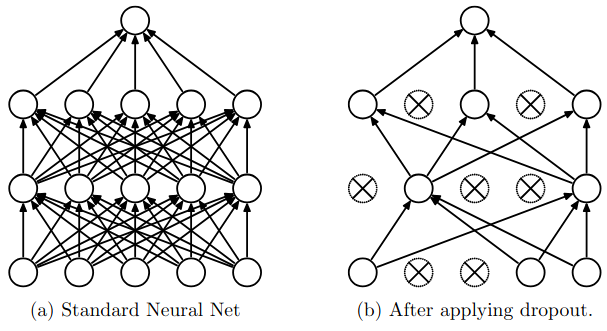
\includegraphics[width=\linewidth]{images/U7.png}
    \label{fig:Scaled Dot Product Attention}
    \vspace{-10pt}
\end{wrapfigure}
Dropout is a regularization technique originally introduced to reduce overfitting and prevent co-adaptation of neurons in standard neural networks. During training, each hidden unit is independently \textit{dropped} (i.e., set to zero) with probability $p$. For each mini-batch, a binary mask $m^{(l)}$ is sampled for every layer $l$:
\[
h_{\text{dropped}}^{(l)} = m^{(l)} \odot h^{(l)},
\qquad
m^{(l)}_i \sim \text{Bernoulli}(1 - p).
\]
This forces the network to learn redundant and robust feature representations, since the model cannot rely on the presence of any single neuron.

At inference time, the dropout noise is typically \emph{disabled}, meaning that the full network is used without masking any activations. To ensure consistency with the expected activations during training, outputs are rescaled by a factor of $(1 - p)$, which maintains the same magnitude as in the stochastic training regime.

Thus, dropout acts as an implicit ensemble of many subnetworks, improving robustness and reducing overfitting at essentially no additional computational cost during training.


\subsection{Monte Carlo Dropout (MC Dropout)}
\begin{wrapfigure}{r}{0.4\textwidth}
    \centering
    \vspace{-10pt}
    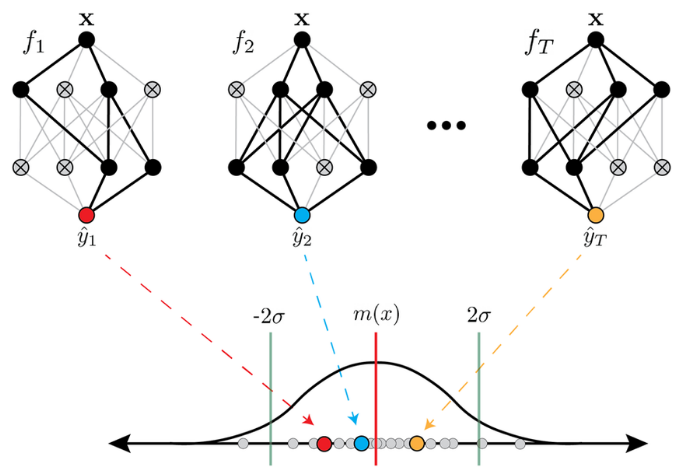
\includegraphics[width=\linewidth]{images/U8.png}
    \label{fig:Scaled Dot Product Attention}
    \vspace{-10pt}
\end{wrapfigure}

BNNs are very useful, but they have a drawback: they require changing the training paradigm and training an entirely different type of network. In many practical scenarios, however, we already have a standard deterministic neural network, and it would be convenient to have a method to make such a network stochastic without redesigning it. This can be achieved through MC Dropout.
Monte Carlo Dropout \ extends the classical dropout mechanism to provide an efficient approximation to Bayesian inference in neural networks. The key idea is to interpret dropout as a variational approximation to a Bayesian neural network, enabling uncertainty estimation without the heavy computational cost of full Bayesian methods.

\textbf{Idea.}  
Instead of disabling dropout at test time, MC Dropout keeps it active and performs multiple stochastic forward passes. Each pass corresponds to sampling a different dropout mask, effectively drawing a sample from an approximate posterior over the model weights.

\textbf{Procedure.}
\begin{enumerate}
    \item Train a standard neural network using dropout as usual.
    \item At test time, leave dropout \emph{enabled} instead of turning it off.
    \item Perform $T$ stochastic forward passes, each with newly sampled dropout masks:
    \[
    f^{(t)}(x) = f(x; \theta, m_1^{(t)}, \ldots, m_L^{(t)}),
    \qquad t = 1, \ldots, T.
    \]
    \item Estimate the predictive mean:
    \[
    \hat{\mu}(x) = \frac{1}{T} \sum_{t=1}^{T} f^{(t)}(x).
    \]
    \item Estimate the predictive covariance:
    \[
    \widehat{\mathrm{Cov}}[y \mid x, D] = 
    \frac{1}{T} \sum_{t=1}^{T} 
    f^{(t)}(x)f^{(t)}(x)^\top
    - 
    \hat{\mu}(x)\hat{\mu}(x)^\top 
    + \tau^{-1} I,
    \]
    where $\tau^{-1}$ is the assumed observation noise variance.
\end{enumerate}

The variability across the stochastic outputs $f^{(t)}(x)$ captures \textbf{epistemic uncertainty}, since it reflects sensitivity to different sampled subnetworks. Model uncertainty can be quantified through the entropy of the predictive distribution, variation ratios, or the predictive covariance above.

The \textbf{Benefits} of the Mont-Carlo Dropout are:
\begin{compactitemize}
    \item No modification to the training procedure is required.
    \item Computational overhead is modest: only multiple forward passes are needed.
    \item Provides a practical approximation to Bayesian uncertainty without training multiple deterministic models (as in Deep Ensembles).
\end{compactitemize}

\section{Reliable Uncertainty Measures}

\subsection{Confidence from the Predicted Probability}

A very common and simple approach to estimate how confident a neural network is about a prediction is to look at the highest output of the Softmax layer.
Given a classification problem with $K$ classes, the network produces a vector of predicted probabilities
\[
\mathbf{p}(x) = [p_1(x), p_2(x), \dots, p_K(x)],
\]
where $p_k(x)$ represents the predicted probability that the input $x$ belongs to class $k$.

For instance, consider the prediction
\[
[0.05,\, 0.10,\, 0.80,\, 0.05].
\]
The highest value is $0.80$, corresponding to class 3. In this case, we would say that the model is \emph{80\% confident} that the input belongs to class 3.

This notion of confidence is intuitive. If the maximum predicted probability is close to $1$, the model appears very certain about its decision. Conversely, if the maximum probability is low, for example around $0.4$ or $0.5$, the prediction is ambiguous and several classes compete with similar scores.

However, this interpretation relies on the implicit assumption that Softmax outputs represent meaningful probabilities. Unfortunately, this assumption is often violated.

\subsection{Miscalibration}
\begin{wrapfigure}{r}{0.5\textwidth}
    \centering
    \vspace{-10pt}
    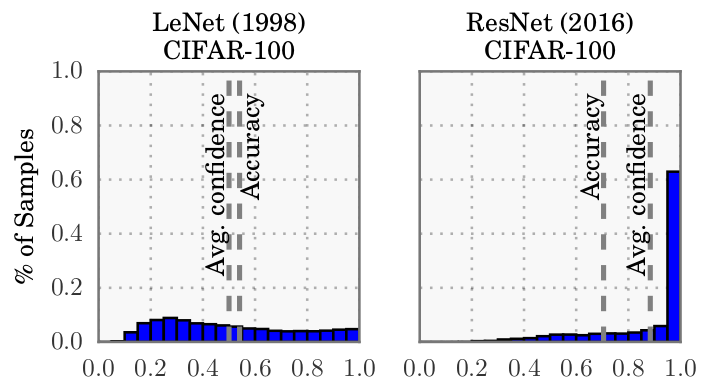
\includegraphics[width=\linewidth]{images/V1.png}
    \label{fig:Scaled Dot Product Attention}
    \vspace{-10pt}
\end{wrapfigure}
The main limitation of using the maximum Softmax probability as a confidence estimate is that this quantity does not necessarily reflect the true probability of making a correct prediction.

Given a dataset $\{x_i\}_{i=1}^N$, the confidence of a model on a single input $x_i$ is typically defined as
\[
\mathrm{conf}(x_i) = \max_{k \in \{1,\dots,K\}} p_\theta(y = k \mid x_i),
\]
that is, the maximum predicted probability among all classes.

At the dataset level, model confidence is often summarized by the \emph{average confidence}, defined as
\[
\frac{1}{N} \sum_{i=1}^{N} \max_{k \in \{1,\dots,K\}} p_\theta(y = k \mid x_i).
\]

If the model were perfectly calibrated, this average confidence would closely match the empirical accuracy. In practice, however, modern neural networks frequently violate this property. The model may assign very high confidence scores to its predictions even when a significant fraction of them are incorrect.

This discrepancy shows that Softmax outputs should not be interpreted as true posterior probabilities. Instead, they represent normalized scores whose scale is influenced by architectural choices and training procedures. As a result, relying solely on the maximum predicted probability can lead to misleading uncertainty estimates, especially in deep and overparameterized models.

This behavior is largely a consequence of how neural networks are trained.
In supervised classification, the ground-truth label is typically encoded as a one-hot vector, for example
\[
[0,\,0,\,1,\,0,\,0],
\]
where the correct class is assigned probability $1$ and all the others probability $0$.

During training, the network is optimized to match this target distribution, usually by minimizing the cross-entropy loss. As a result, the model is explicitly encouraged to concentrate as much probability mass as possible on a single class, pushing the maximum predicted probability toward $1$.

However, this one-hot target does not represent the true underlying uncertainty of the data-generating process. In many cases, the real posterior distribution over classes is much softer, but the network is never exposed to this information. Consequently, the model learns to approximate an artificially sharp distribution, which explains why high confidence values are often produced even when the prediction is incorrect.

This mismatch between the learned confidence scores and the true likelihood of correctness directly leads to miscalibration.

This effect is further amplified by model complexity.
Smaller and simpler networks tend to produce smoother and more conservative confidence estimates, which are often more reliable. Their confidence values are less extreme and closer to the empirical accuracy, making them, in practice, more \emph{honest} about their uncertainty.

In contrast, large and highly overparameterized architectures, such as very deep models, have sufficient capacity not only to fit the training data correctly but also to push the predicted probabilities toward extreme values. In this regime, the network learns to strongly commit to its predictions, assigning high confidence scores even in situations where uncertainty should be present.

This behavior can be interpreted as a form of overfitting at the level of confidence rather than accuracy. While the overall classification performance may improve, the predicted probability distribution becomes increasingly sharp and less representative of the true underlying uncertainty. As a consequence, the model appears highly confident even when it is wrong.

For this reason, older or smaller architectures often exhibit better calibration: not because they are more accurate, but because their limited capacity prevents them from producing overly confident predictions. Their confidence estimates are smoother, more moderate, and therefore more aligned with the true likelihood of correctness.

\subsubsection{A Calibration Question}

Consider the following question. Suppose we collect all the samples in a dataset for which the model’s confidence, defined as the maximum predicted probability, lies in the interval $[0.45, 0.55]$, that is, close to $0.5$.

If we take 100 such samples, how many of them should we expect to be classified correctly?

The answer is \emph{approximately 50}, but this holds if and only if the model is perfectly calibrated. In a well-calibrated model, predictions with confidence $c$ are correct approximately $c \times 100\%$ of the time. When this property does not hold, the confidence values cannot be trusted as measures of uncertainty.

\subsection{Reliability Diagrams}

Reliability diagrams are a standard tool used to visualize and evaluate the calibration of a model. The idea is to group predictions into confidence bins, for example $[0.0,0.1], [0.1,0.2], \dots, [0.9,1.0]$, according to their maximum predicted probability.

For each bin, two quantities are computed: the average confidence of the samples in the bin and the empirical accuracy, defined as the fraction of correctly predicted samples. These values are then plotted against each other.

If a model is perfectly calibrated, the points in the reliability diagram lie on the diagonal line $y=x$. Any deviation from this diagonal indicates miscalibration. When the accuracy is consistently below the confidence, the model is overconfident; when it is above, the model is underconfident.
\begin{figure}[H]
    \centering
    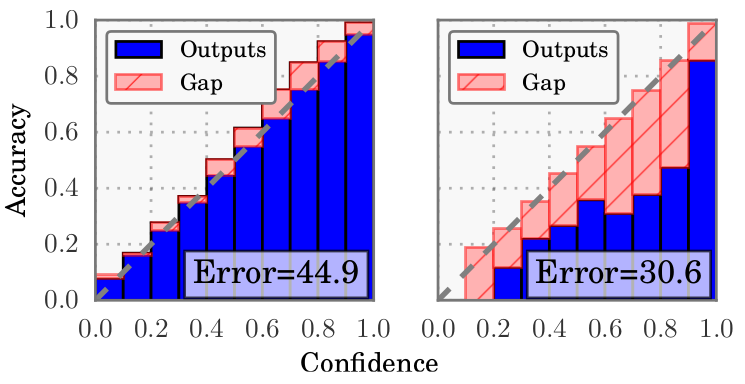
\includegraphics[width=0.5\textwidth]{images/V2.png}
    \label{fig:Scaled Dot Product Attention}
\end{figure}

Empirical results on datasets such as CIFAR-100 show that deep architectures like ResNet (right in the image above), despite achieving significantly higher accuracy than older models such as LeNet (left in the image above), are often much more miscalibrated. In contrast, simpler and older networks tend to produce confidence estimates that better reflect their true correctness likelihood, even if their overall accuracy is lower.

\subsection{Expected Calibration Error (ECE)}

While reliability diagrams provide an intuitive and visual way to assess calibration, it is often useful to summarize miscalibration with a single numerical metric. The most commonly used measure for this purpose is the \emph{Expected Calibration Error} (ECE).

The goal of ECE is to quantify how far the model’s predicted confidence is from its actual empirical accuracy. To compute ECE, predictions are first partitioned into $M$ confidence bins, typically obtained by dividing the interval $[0,1]$ into equally spaced ranges such as $[0.0,0.1], [0.1,0.2], \dots, [0.9,1.0]$. Each sample is assigned to a bin based on its predicted confidence, defined as the maximum Softmax probability.

For each bin $B_m$, two quantities are computed. The accuracy of the bin is defined as
\[
\mathrm{acc}(B_m) = \frac{1}{|B_m|} \sum_{x_i \in B_m} \mathbb{I}\{\hat{y}_i = y_i\},
\]
that is, the fraction of correctly classified samples in the bin. The average confidence of the bin is defined as
\[
\mathrm{conf}(B_m) = \frac{1}{|B_m|} \sum_{x_i \in B_m} \max_k p_\theta(y = k \mid x_i).
\]

The Expected Calibration Error is then defined as a weighted average of the absolute difference between accuracy and confidence across all bins:
\[
\mathrm{ECE} = \sum_{m=1}^{M} \frac{|B_m|}{n} \, \big| \mathrm{acc}(B_m) - \mathrm{conf}(B_m) \big|,
\]
where $n$ is the total number of samples.

An ECE value equal to zero corresponds to perfect calibration, meaning that for every confidence level the predicted confidence matches the empirical accuracy. Larger ECE values indicate increasing degrees of miscalibration. Intuitively, ECE measures the average vertical distance between the reliability diagram and the diagonal line representing ideal calibration.
\begin{figure}[H]
    \centering
    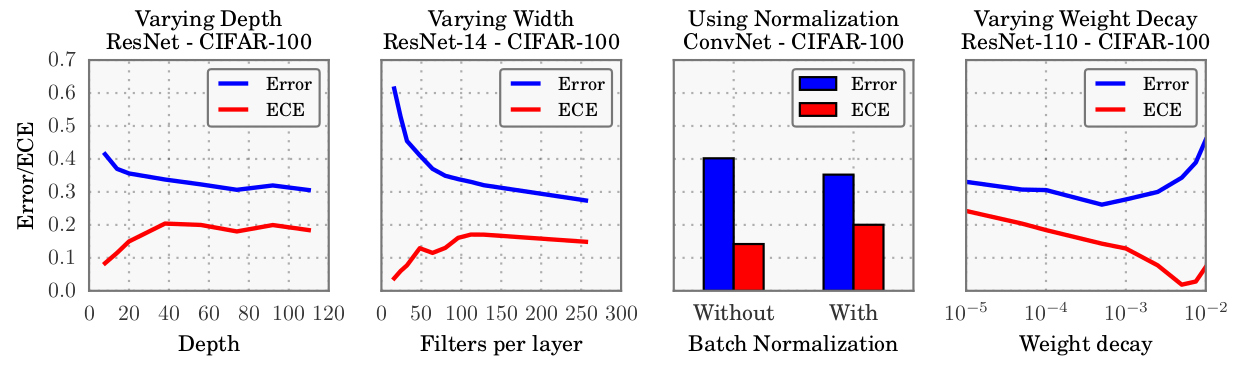
\includegraphics[width=1\textwidth]{images/U9.png}
    \label{fig:MHA2}
\end{figure}

\subsection{Temperature Scaling}

Temperature scaling is a simple yet effective post-processing technique used to improve the calibration of a trained classifier without affecting its predictive accuracy. The key idea is to modify the confidence of the predictions while leaving the predicted class unchanged.

Let $\mathbf{z} = (z_1, \dots, z_K)$ denote the logits produced by the network before the Softmax layer. Temperature scaling introduces a single scalar parameter $T > 0$, called the \emph{temperature}, and rescales the logits before applying Softmax:
\[
p_\theta(y = k \mid x) =
\frac{\exp(z_k / T)}{\sum_{j=1}^{K} \exp(z_j / T)}.
\]
\begin{wrapfigure}{r}{0.4\textwidth}
    \centering
    \vspace{-10pt}
    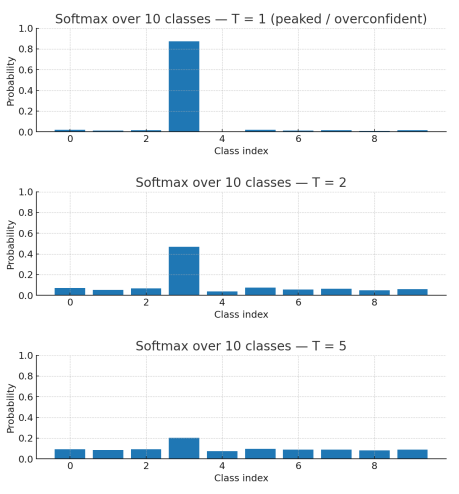
\includegraphics[width=\linewidth]{images/U10.png}
    \label{fig:Scaled Dot Product Attention}
    \vspace{-10pt}
\end{wrapfigure}
When $T = 1$, the standard Softmax is recovered. For $T > 1$, the logits are divided by a value greater than one, resulting in a softer probability distribution. In this case, the maximum predicted probability is reduced, leading to lower and more conservative confidence scores. Importantly, the ordering of the logits is preserved, so the predicted class does not change.

The temperature parameter is learned after training, using a held-out validation set. Specifically, $T$ is optimized by minimizing the negative log-likelihood of the validation data, while keeping all model parameters fixed. As a consequence, temperature scaling does not modify the classifier itself but only rescales the confidence values of its predictions.

An important advantage of temperature scaling is that it improves calibration without altering the model’s accuracy. Since the predicted labels remain identical, performance metrics such as accuracy are unchanged, while the predicted probabilities become more aligned with the empirical correctness likelihood.


\subsection{Brier Score}

The Brier Score is a commonly used metric to evaluate the quality of probabilistic predictions in both binary and multi-class classification settings. Unlike accuracy, which only evaluates whether the predicted class is correct, the Brier Score explicitly measures how close the predicted probability distribution is to the true target distribution.

Formally, for a dataset of $N$ examples and $K$ classes, the Brier Score is defined as
\[
\mathrm{BS} = \frac{1}{N} \sum_{i=1}^{N} \sum_{k=1}^{K}
\big( p_{i,k} - y_{i,k} \big)^2,
\]
where $p_{i,k}$ denotes the probability predicted by the model for class $k$ on example $i$, and $y_{i,k}$ is the corresponding one-hot encoded ground-truth label.

The Brier Score computes the mean squared difference between predicted probabilities and the true outcomes. Intuitively, it penalizes both incorrect predictions and poorly calibrated confidence estimates. Confident but wrong predictions result in a large penalty, while well-calibrated and accurate probability estimates yield low scores.

Lower Brier Score values indicate better probabilistic predictions. In the binary classification setting, the score ranges from $0$, corresponding to perfect predictions, to $1$, corresponding to maximally incorrect and overconfident predictions. In the multi-class case, the range depends on the number of classes but the interpretation remains the same.

An important property of the Brier Score is that it is a \emph{proper scoring rule}. This means that the score is minimized when the predicted probabilities match the true underlying data distribution, thereby encouraging honest and well-calibrated probability estimates. Moreover, the Brier Score is sensitive not only to calibration but also to refinement, capturing both how accurate and how sharp the predicted probability distributions are.

\subsection{Out-of-Distribution Detection}

Out-of-distribution (OOD) detection aims at identifying inputs that differ significantly from the data distribution used during training. The objective is to detect these inputs at test time so that the model can abstain from making a prediction or trigger a fallback mechanism.

This problem is particularly important because deep neural networks are known to produce highly confident predictions even for inputs that are completely unrelated to the training data, such as random noise or samples coming from a different domain. In safety-critical applications, including medical diagnosis and autonomous driving, such overconfident behavior on OOD inputs can lead to severe and potentially dangerous errors.

OOD detection therefore complements uncertainty estimation and calibration: even a well-calibrated model on in-distribution data may behave unpredictably when evaluated far outside its training support.

\subsubsection{ODIN}

ODIN is a post-hoc method for OOD detection that operates on a trained classifier, without requiring retraining or architectural changes. Its goal is to increase the separation between in-distribution (ID) and out-of-distribution samples by exploiting differences in how the model reacts to small input perturbations.

The method combines two key components. First, temperature scaling is applied to the logits, using a temperature value $T > 1$ to soften the Softmax output. This reduces overconfidence and amplifies relative differences in confidence between ID and OOD inputs.

Second, a small, carefully chosen perturbation is added to the input. Specifically, the input $x$ is modified as
\[
\tilde{x} = x + \epsilon \, \mathrm{sign} \left( \nabla_x \log p(y_{\max} \mid x; T) \right),
\]
where $y_{\max}$ is the class with maximum predicted probability under temperature-scaled Softmax, and $\epsilon$ controls the perturbation magnitude.

This step resembles an adversarial update, but with the opposite objective: instead of reducing confidence, the perturbation is designed to increase the model’s confidence in its current prediction.

The key intuition behind ODIN is that this perturbation has a different effect on ID and OOD samples. For in-distribution inputs, the perturbation tends to align with meaningful features learned during training, producing a noticeable increase in the maximum Softmax probability. In contrast, OOD inputs typically lie in regions of the input space that the model does not understand well. As a consequence, even after the perturbation, their logits do not align strongly with any learned pattern, and the Softmax confidence increases only marginally.

At test time, both temperature scaling and input perturbation are applied, and the maximum Softmax probability computed on $\tilde{x}$ is used as an OOD score. By comparing this score to a predefined threshold, the model can flag inputs that are likely to be out-of-distribution. The combined effect of temperature scaling and input perturbation widens the confidence gap between ID and OOD samples, making them easier to separate.

\chapter{Self-Supervised Learning}

\section{Introduction}
Self-Supervised Learning (SSL) is  a particular type of representation learning that enables learning good data representation from \textbf{unlabelled} dataset.

The \textbf{idea} of the SSL is to constructing supervised learning task out of unsupervised dataset.

This make sense for two reason:
\begin{compactitemize}
    \item Data labelling is expensive; thus, the high-quality labeled dataset is limited.
    \item Learning good representation makes transferring useful information to various downstream tasks.
\end{compactitemize}
\begin{figure}[H]
    \centering
    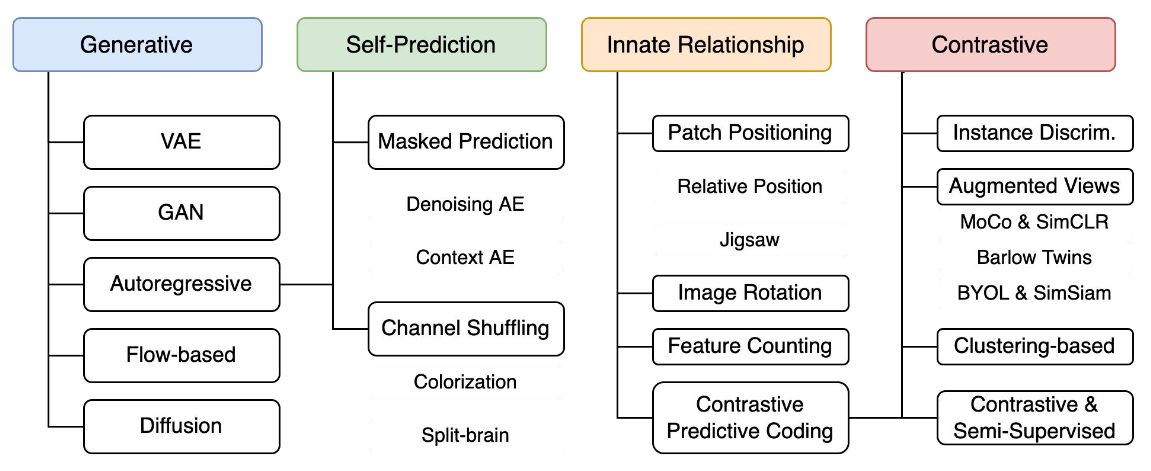
\includegraphics[width=1\textwidth]{images/SS1.png}
    \label{fig:MHA2}
\end{figure}

\subsection{Self-Supervised Learning vs Generative Learning}
Often, we are not really interested to generate pixel-level detail. Instead we are more interested to learn only high-level semantic features through \textbf{pretext task}.
\begin{figure}[H]
    \centering
    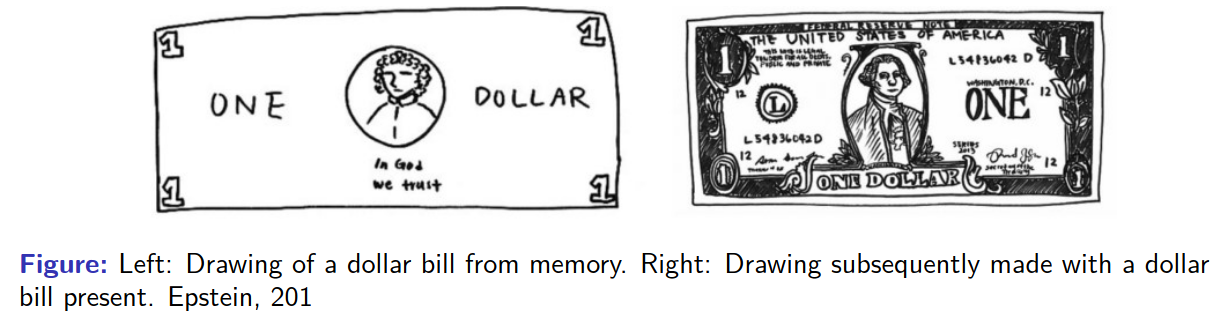
\includegraphics[width=0.85\textwidth]{images/SS2.png}
    \label{fig:MHA2}
\end{figure}

\subsection{Self-Supervised Learning through Pretext Tasks}

Self-supervised learning aims to learn high-level semantic representations from data without relying on manually annotated labels. This is achieved through the use of \textbf{pretext tasks}, which are automatically generated tasks designed to encourage the model to extract meaningful and general features from the data.

One of the main characteristics of a pretext task is that it allows labels to be generated automatically, without any human intervention (e.g., image rotation, colorization, or jigsaw puzzles).

As an example, consider the following \textbf{pretext task}: given an image of a bird, the image is rotated by a certain angle (e.g., $0^\circ$, $90^\circ$, $180^\circ$, $270^\circ$), and the model is trained to \textbf{predict} which rotation has been applied. This results in a simple 4-class classification problem.

In this scenario, the model is a standard \textbf{Convolutional Neural Network (CNN)}. After training the CNN on the pretext task, the network learns to extract useful visual features that capture the structure and semantics of the images. Once training is complete, the feature extractor (i.e., the convolutional layers) can be detached and reused as part of a new model for a downstream task.

Specifically, the pretrained feature extractor is connected to a new Multi-Layer Perceptron (MLP) designed for the target task. Since the CNN has already learned informative representations through the pretext task, only a relatively small amount of labeled data is required to train the new model. This approach partially addresses the problem of limited labeled data by leveraging large amounts of unlabeled data during pretraining.
\begin{figure}[H]
    \centering
    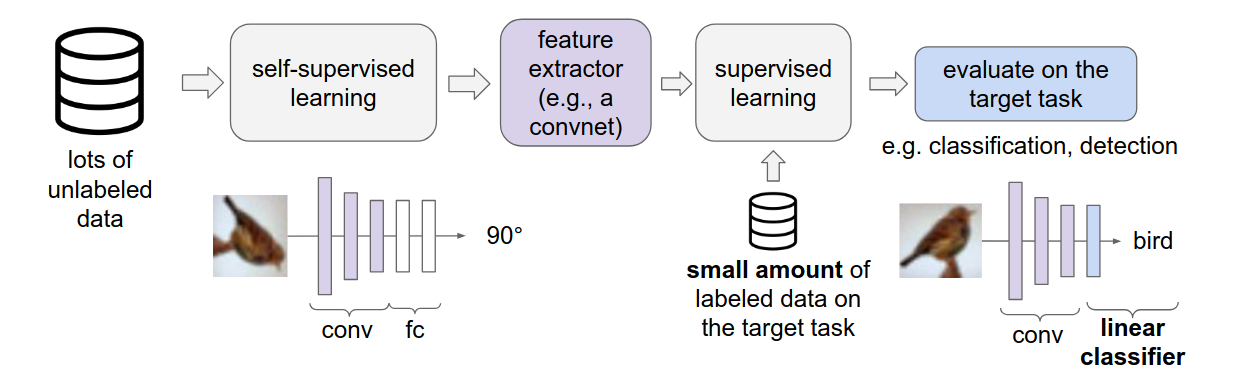
\includegraphics[width=0.9\textwidth]{images/SS3.png}
    \label{fig:MHA2}
\end{figure}
Predicting image rotations is an effective pretext task because it encourages the model to learn meaningful visual representations rather than focusing on low-level cues. In order to correctly infer the rotation applied to an image, the model must develop a form of visual commonsense, that is, an understanding of how objects typically appear in their canonical, unperturbed orientation.

Indeed, recognizing whether an object is upright, upside-down, or rotated by a specific angle requires the network to capture high-level semantic information such as object shape, part configuration, and spatial relationships between components. For example, correctly identifying that an animal is upside-down implies understanding where its head, limbs, and body are normally located. This prevents the model from relying solely on trivial pixel-level statistics and instead pushes it toward learning semantically rich and transferable features.

As a result, rotation prediction acts as a strong supervisory signal without requiring manual annotations. The features learned during this pretraining phase are general and robust, making them well-suited for downstream tasks such as image classification, object detection, or segmentation, even when only a limited amount of labeled data is available.
\begin{wrapfigure}{r}{0.5\textwidth}
    \centering
    \vspace{-10pt}
    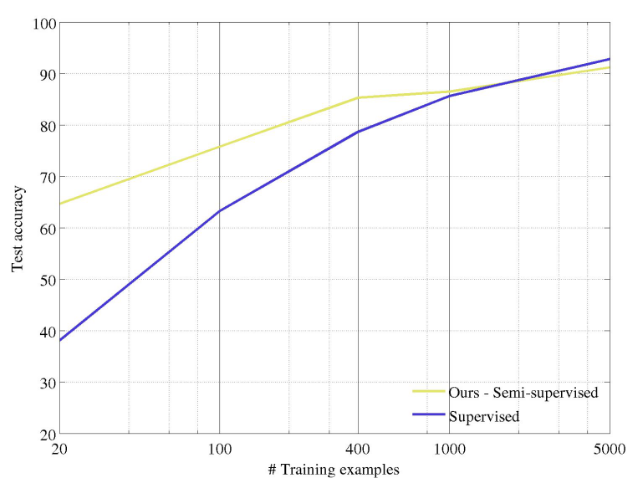
\includegraphics[width=\linewidth]{images/SS4.png}
    \label{fig:Scaled Dot Product Attention}
    \vspace{-10pt}
\end{wrapfigure}
The figure shows that \textbf{self-supervised pretraining} based on rotation prediction enables the model to learn \textbf{robust and transferable visual features}. During the downstream supervised phase, the early layers (\textbf{conv1 and conv2}) are \textbf{frozen}, while only the higher-level layers (\textbf{conv3 and the linear classifier}) are trained using a \textbf{small subset of labeled data}. This setup demonstrates that the representations learned through the pretext task are sufficiently informative to achieve strong performance even with limited supervision.

\section{SLL through intra-example relationships}

\subsection{Pretext Task: Solving ``Jigsaw Puzzles''}

Learning the spatial relationships among image patches is an effective strategy for self-supervised representation learning. In this context, the pretext task consists of dividing an image into a set of patches and training a model to predict their correct relative positions or permutations. Early approaches include predicting the relative position between pairs of patches  and solving jigsaw puzzles constructed from shuffled image patches.
\begin{figure}[H]
    \centering
    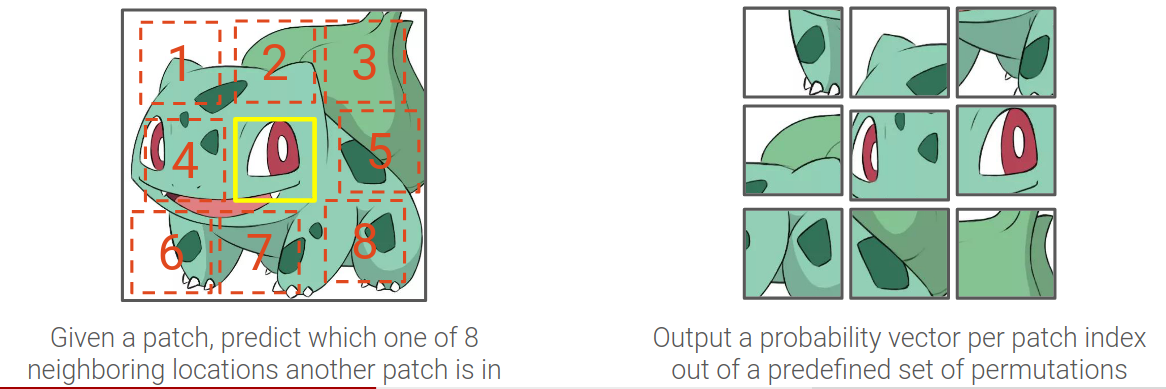
\includegraphics[width=0.9\textwidth]{images/SS5.png}
    \label{fig:MHA2}
\end{figure}
The intuition behind the jigsaw puzzle task is that, to correctly reassemble the image, the model must understand that objects are composed of meaningful parts and learn how these parts are spatially arranged. This encourages the network to capture semantic information about object structure rather than relying on low-level visual cues.

A key challenge of this approach is the inherent ambiguity when considering each patch independently, as multiple configurations may appear locally plausible. To address this issue, the model observes all patches jointly, framing the problem as a global permutation prediction task. Since the placement of each patch is mutually exclusive, jointly reasoning over all tiles significantly reduces ambiguity and leads to the learning of more coherent and informative visual representations .
\begin{figure}[H]
    \centering
    \begin{minipage}{0.35\textwidth}
        \centering
        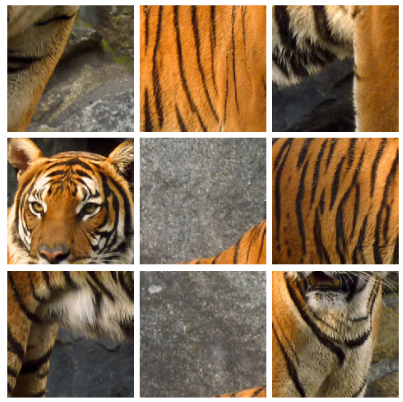
\includegraphics[width=\textwidth]{images/SS6.png}
        \label{fig:Residuals}
    \end{minipage}
    \label{fig:TS_Residuals}
    \hfill
    \begin{minipage}{0.35\textwidth}
        \centering
        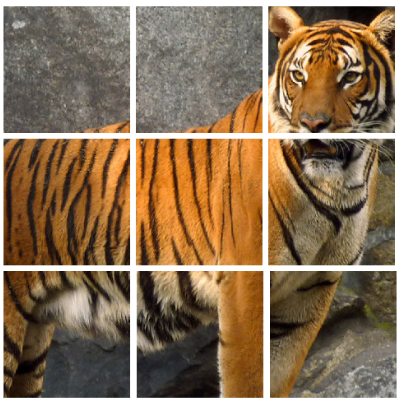
\includegraphics[width=\textwidth]{images/SS7.png}
        \label{fig:Residuals}
    \end{minipage}
    \label{fig:TS_Residuals}
\end{figure}

\subsection{Pretext Task: Predicting Relative Patch Locations}

Predicting the relative spatial arrangement of image patches is an early and influential pretext task for self-supervised representation learning. Given a large collection of unlabeled images, random pairs of patches are extracted from each image and used as input to the model. One patch is treated as a reference, while the second patch is sampled from a neighboring region at a relative position drawn from a predefined set.

The pretext task consists of training a model to predict the relative position of the second patch with respect to the first (e.g., top, bottom, left, right, or diagonal), framing the problem as a classification task. This setup does not require any manual annotations, as the relative spatial relationship between patches is automatically determined during data generation.

The underlying hypothesis is that performing well on this task requires the model to move beyond low-level texture cues and instead learn semantically meaningful representations. In particular, the model is encouraged to recognize objects, their constituent parts, and their typical spatial configurations, since understanding how parts of an object are arranged is crucial for correctly reasoning about relative patch locations.
\begin{figure}[H]
    \centering
    \begin{minipage}{0.5\textwidth}
        \centering
        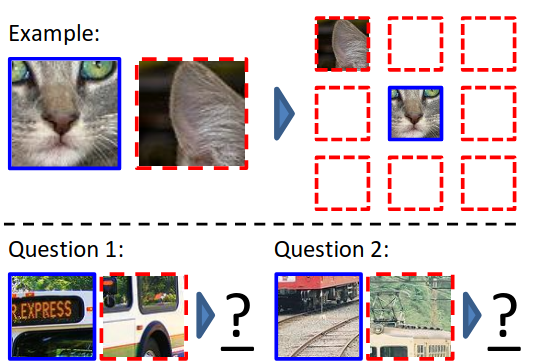
\includegraphics[width=\textwidth]{images/SS8.png}
        \label{fig:Residuals}
    \end{minipage}
    \label{fig:TS_Residuals}
    \hfill
    \begin{minipage}{0.4\textwidth}
        \centering
        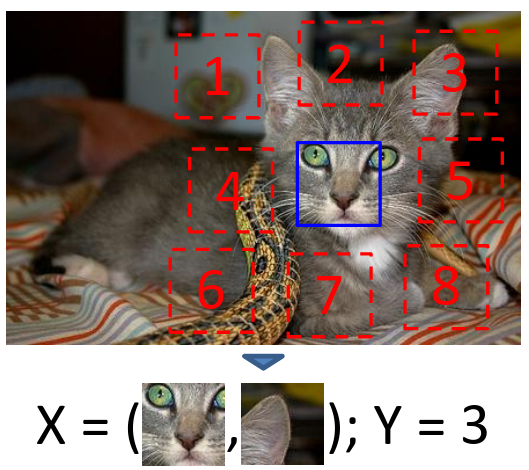
\includegraphics[width=\textwidth]{images/SS9.png}
        \label{fig:Residuals}
    \end{minipage}
    \label{fig:TS_Residuals}
\end{figure}

\subsection{Pretext Tasks: Colorization}
\begin{wrapfigure}{r}{0.2\textwidth}
    \centering
    \vspace{-10pt}
    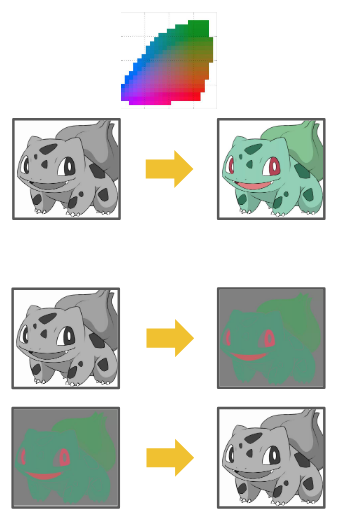
\includegraphics[width=\linewidth]{images/SS10.png}
    \label{fig:Scaled Dot Product Attention}
    \vspace{-10pt}
\end{wrapfigure}
Image colorization is a powerful self-supervised pretext task that consists of predicting color information from grayscale images. In this setting, supervision is obtained directly from the data, since color images can be automatically converted to grayscale. One representative approach is proposed by Zhang et al., where the model is trained to predict the discretized color values in the CIE Lab color space given only the luminance channel. The task is formulated as a classification problem over color bins, which helps the model capture multimodal color distributions.

Colorization encourages the network to learn high-level semantic features, as assigning plausible colors often requires understanding object identity, material properties, and scene context. In particular, correctly colorizing an image implicitly forces the model to distinguish between different object parts (e.g., eyes, skin, hair), to reason about shapes and boundaries, and to separate foreground objects from the background. This process leads the network to capture meaningful structural and spatial information rather than relying solely on low-level texture cues.

A generalization of this idea is the \emph{split-brain autoencoder} introduced by Zhang et al. In this framework, the input channels are divided into two complementary subsets, and the model is trained to predict one subset from the other. For example, the network may predict chrominance from luminance, or more generally, infer color, depth, or other modalities from available visual information. By forcing different subnetworks to learn from partial observations, this approach further promotes the learning of robust and semantically rich representations.

Beyond representation learning, colorization models also have practical applications. Since they are trained using artificially generated grayscale images, they can be directly applied to real legacy black-and-white photographs, producing visually plausible colorized results, as demonstrated in \emph{Colorful Image Colorization} by Zhang et al.
\begin{figure}[H]
    \centering
    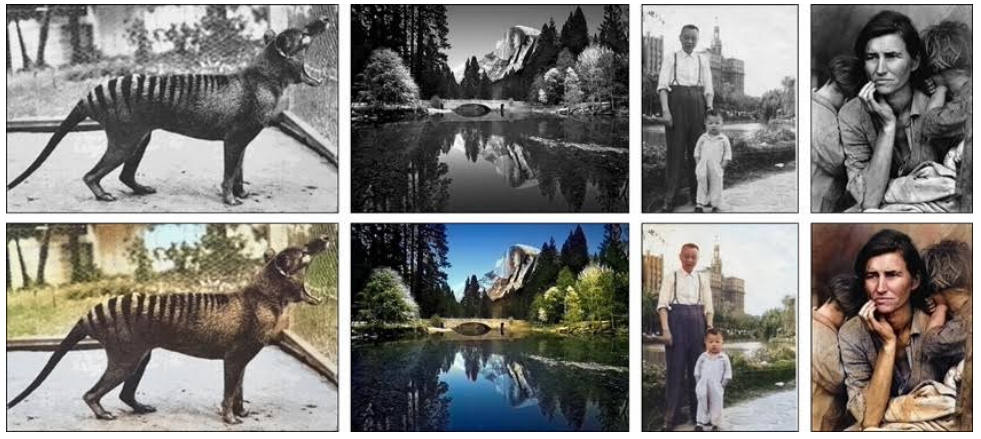
\includegraphics[width=0.7\textwidth]{images/SS11.png}
    \label{fig:MHA2}
\end{figure}

\section{Self-Prediction}
\begin{wrapfigure}{r}{0.25\textwidth}
    \centering
    \vspace{-10pt}
    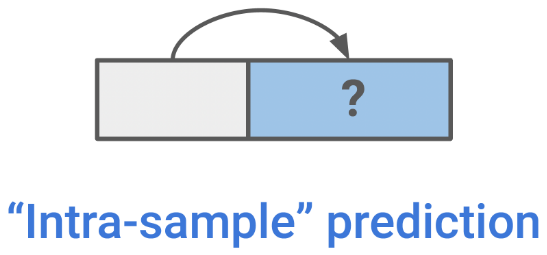
\includegraphics[width=\linewidth]{images/SS12.png}
    \label{fig:Scaled Dot Product Attention}
    \vspace{-10pt}
\end{wrapfigure}
Self-prediction is a branch of \textbf{self-supervised learning} in which, given an individual data sample, the learning task consists of predicting one part of the sample from the remaining parts. The key idea is to artificially define a prediction problem \emph{within} each data sample, without relying on externally provided labels.

\begin{figure}[H]
    \centering
    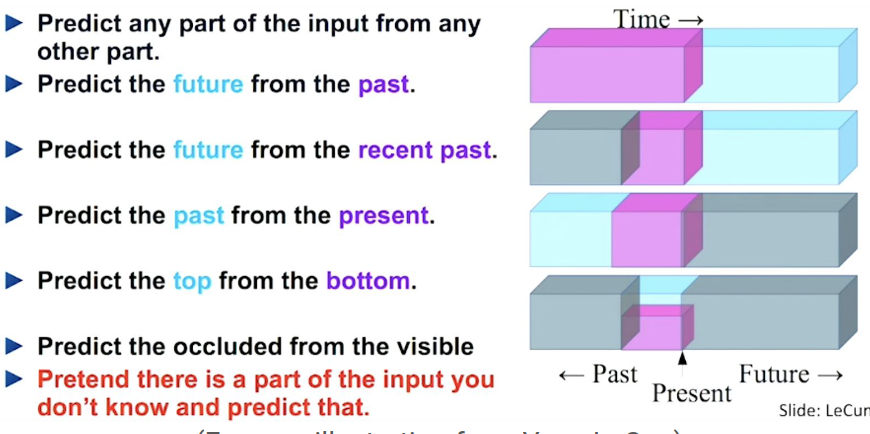
\includegraphics[width=0.6\textwidth]{images/SS13.png}
    \label{fig:MHA2}
\end{figure}
More specifically, a portion of the data is treated as if it were \textbf{missing}, even though it is actually available. The neural network is then trained to predict this missing part using the observed portion of the sample. By doing so, the model is forced to learn meaningful internal representations that capture the structure and dependencies of the data.

In general, self-prediction methods construct prediction tasks directly from the data by pretending that certain parts are unknown and using the remaining parts as input. This principle applies across different data modalities (e.g., images, audio, text) and forms the foundation of several successful self-supervised approaches.

Self-prediction methods can be broadly categorized into three main classes:
\begin{compactitemize}
    \item \textbf{Masked generation}
    \item \textbf{Autoregressive generation}
    \item \textbf{Hybrid self-prediction}
\end{compactitemize}

\subsection{Masked Generation}

Masked generation is a self-prediction strategy in which a random portion of the input data is masked out and treated as missing, independently of any natural ordering in the data. The model is trained to predict the masked portion using the remaining unmasked information, thereby learning dependencies and structure within the data.

This paradigm can be applied across different modalities. In natural language processing, a prominent example is \textbf{masked language modeling}, as used in BERT, where randomly selected tokens are masked and the model is trained to predict them from the surrounding context. In computer vision, masked generation includes tasks such as image inpainting and masked patch prediction, including recent approaches like \textbf{Masked AutoEncoders (MAEs)}.
\begin{figure}[H]
    \centering
    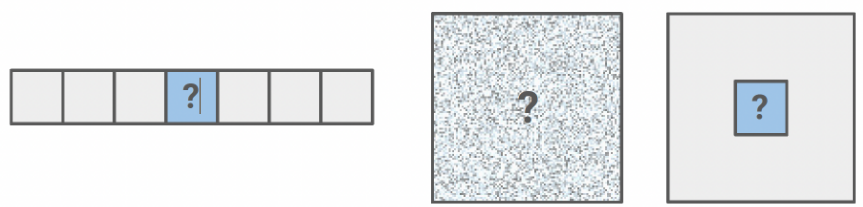
\includegraphics[width=0.6\textwidth]{images/SS14.png}
    \label{fig:MHA2}
\end{figure}
\subsubsection{Self-prediction by Inpainting}

Self-prediction by inpainting consists of predicting the content of an arbitrary missing region in an image based on its surrounding context. In this setting, a portion of the image is removed, and the model is trained to reconstruct the missing pixels using the visible parts of the image \cite{Pathak2016}.

To succeed at this task, the model must capture both local appearance cues and global semantic information. In particular, it needs to understand the overall image content in order to produce a plausible hypothesis for the missing region. As a result, inpainting encourages the learning of representations that encode not only textures and low-level visual features, but also object structure, spatial relationships, and semantic coherence.
\begin{figure}[H]
    \centering
    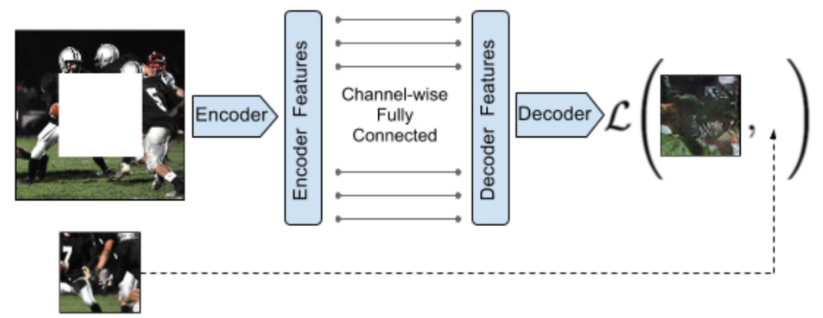
\includegraphics[width=0.7\textwidth]{images/SS15.png}
    \label{fig:MHA2}
\end{figure}
\subsubsection{Self-prediction through Masked AutoEncoders}

Masked AutoEncoders (MAEs) are a self-prediction approach in which random patches of an input image are masked, and the model is trained to reconstruct the missing patches in pixel space. Unlike traditional autoencoders, MAEs adopt an \textbf{asymmetric encoder-decoder architecture}.

The encoder processes only the visible patches and produces a latent representation without using mask tokens, making it computationally efficient. The decoder then takes this latent representation together with mask tokens and reconstructs the full image, including the missing patches. By reconstructing heavily masked inputs, MAEs force the model to learn strong and semantically meaningful visual representations that are well suited for downstream tasks.
\begin{figure}[H]
    \centering
    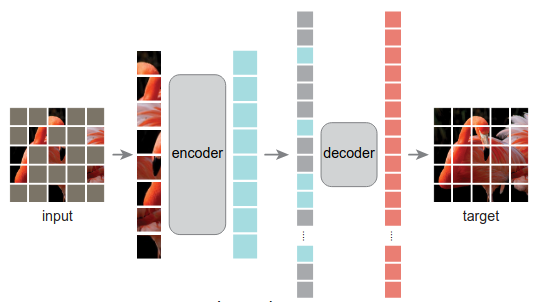
\includegraphics[width=0.6\textwidth]{images/SS16.png}
    \label{fig:MHA2}
\end{figure}
\subsection{Autoregressive Generation}

Autoregressive generation is a self-prediction strategy in which the model predicts future elements of a data sample based on previously observed elements. This approach explicitly exploits the inherent sequential structure of the data and models the joint distribution as a product of conditional probabilities.

Autoregressive models are widely used in domains where data has a natural ordering. Examples include audio generation (e.g., WaveNet, WaveRNN), autoregressive language modeling (e.g., GPT, XLNet), and image modeling by imposing an artificial raster-scan order on pixels or patches (e.g., PixelCNN, PixelRNN, and iGPT).
\begin{figure}[H]
    \centering
    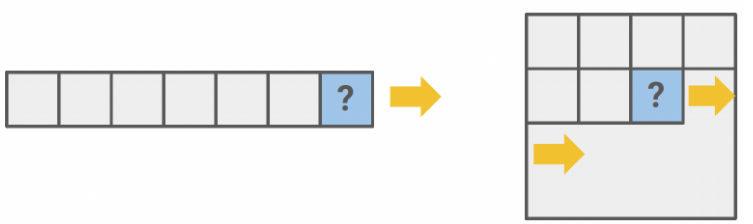
\includegraphics[width=0.6\textwidth]{images/SS17.png}
    \label{fig:MHA2}
\end{figure}

\section{Contrastive Learning}
\section{Contrastive Learning}

Pretext tasks play a central role in self-supervised learning, as they encourage models to acquire meaningful visual representations without relying on human-annotated labels. In particular, they push neural networks to develop a form of \textbf{visual common sense}, enabling the extraction of high-level semantic information that can be effectively reused for downstream tasks. To successfully solve a pretext task, the model is forced to learn informative features of natural images, such as object structure and semantic categories, rather than relying on superficial visual cues. Importantly, the final goal is not to maximize performance on the pretext task itself, but to learn representations that are \textbf{useful and transferable} to downstream applications such as classification, detection, or segmentation.

Despite their effectiveness, pretext-task-based approaches present several limitations. Designing suitable pretext tasks often requires \textbf{significant manual effort} and domain knowledge. Moreover, the learned representations may fail to be sufficiently general, as they can become \textbf{tightly coupled to the specific pretext task} used during training, reducing their applicability across different downstream problems.

These limitations naturally raise the question of whether it is possible to define a more general and task-agnostic self-supervised learning paradigm. \textbf{Contrastive learning} provides a positive answer to this question. Instead of relying on a handcrafted prediction task, contrastive learning learns representations by comparing different views of the data, explicitly encouraging representations of similar samples to be close while pushing apart representations of dissimilar samples. This formulation yields a more flexible and general objective, capable of producing robust and widely transferable visual features.

\begin{figure}[H]
    \centering
    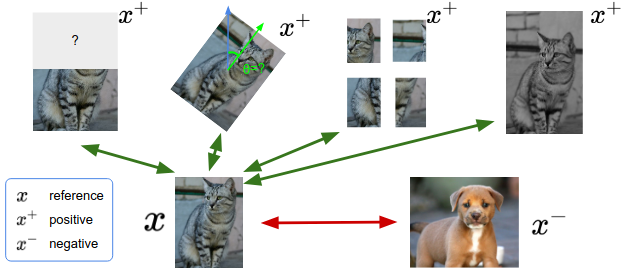
\includegraphics[width=0.8\textwidth]{images/SS18.png}
    \label{fig:MHA2}
\end{figure}

\subsection{Contrastive Representation Learning}

The goal of \textbf{contrastive representation learning} is to learn an embedding space in which semantically similar samples are mapped close to each other, while dissimilar samples are pushed far apart. This objective is achieved by explicitly comparing pairs of samples and enforcing relative similarity constraints in the learned representation space.
\begin{figure}[H]
    \centering
    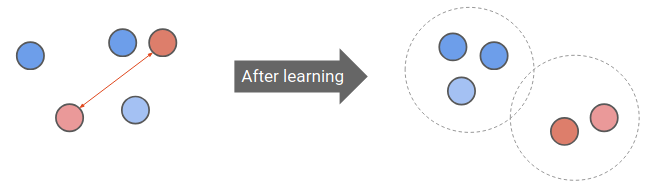
\includegraphics[width=0.6\textwidth]{images/SS20.png}
    \label{fig:MHA2}
\end{figure}
Formally, given an encoder function $f(\cdot;\theta_f)$, a reference sample $x$ (also called an \textbf{anchor}), a \textbf{positive sample} $x^+$ that is semantically related to $x$, and a \textbf{negative sample} $x^-$ that is unrelated, the model is trained such that
\[
\text{score}(f(x), f(x^+)) \gg \text{score}(f(x), f(x^-)).
\]
The score function typically measures similarity in the embedding space, such as cosine similarity or dot product.

Positive samples are usually obtained through \textbf{positive mining strategies}, for example by applying different data augmentations to the same input or by using different views of the same underlying scene or object. Negative samples are drawn from other, unrelated data points within the dataset or the same training batch.

By enforcing these constraints, contrastive learning encourages the encoder to capture high-level semantic features that are invariant to irrelevant transformations, resulting in representations that are robust and highly transferable to downstream tasks.

\subsection{Contrastive Loss}

The contrastive loss was introduced by Chopra et al. as a metric learning objective designed to bring similar samples close in the embedding space while pushing dissimilar samples apart. Unlike self-supervised contrastive learning, this formulation typically assumes the availability of \textbf{labeled data}, where samples from the same class are considered similar and samples from different classes are considered dissimilar.

Given an encoder function $f(\cdot;\theta_f)$ and a pair of labeled samples $(x_i, x_j)$, the contrastive loss is defined as:
\[
\mathcal{L}(x_i, x_j; \theta_f) =
\begin{cases}
\| f(x_i) - f(x_j) \|, & \text{if } i = j ,(minimize) \\
\max\left(0, \alpha - \| f(x_i) - f(x_j) \| \right), & \text{if } i \neq j ,(maximize)
\end{cases}
\]
where $\alpha$ is a positive margin that controls the minimum desired distance between embeddings of samples belonging to different classes.

For positive pairs (i.e., samples from the same class), the loss encourages minimizing the distance between their embeddings. For negative pairs, the loss penalizes embeddings that are closer than the margin $\alpha$. If the distance between two negative samples exceeds the margin, their contribution to the loss is zero.

The introduction of the margin is crucial to prevent \textbf{representation collapse}, a degenerate solution in which all samples are mapped to the same point in the embedding space. By enforcing a minimum separation between negative pairs, contrastive loss promotes a structured and discriminative embedding space.

\subsection{Triplet Loss}

The triplet loss is a metric learning objective that extends the contrastive loss by jointly considering three samples at a time: an \textbf{anchor} sample $x$, a \textbf{positive} sample $x^+$ belonging to the same class as the anchor, and a \textbf{negative} sample $x^-$ belonging to a different class. The objective is to learn an embedding space in which the anchor is closer to the positive sample than to the negative one.

More formally, the desired constraint is that the distance between the anchor and the positive sample is smaller than the distance between the anchor and the negative sample by at least a margin $\alpha$:
\[
\| f(x) - f(x^+) \|_2^2 + \alpha < \| f(x) - f(x^-) \|_2^2.
\]

This constraint is enforced by minimizing the following loss function:
\[
\mathcal{L}(x, x^+, x^-; \theta_f) =
\max\left(0,
\| f(x) - f(x^+) \|_2^2
-
\| f(x) - f(x^-) \|_2^2
+ \alpha
\right).
\]

If the constraint is satisfied, the loss is zero; otherwise, the model is penalized proportionally to how much the margin is violated. By jointly optimizing distances between anchor--positive and anchor--negative pairs, the triplet loss encourages a well-structured and discriminative embedding space.

\begin{figure}[H]
    \centering
    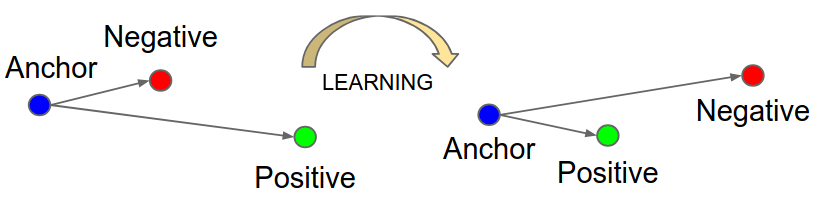
\includegraphics[width=0.6\textwidth]{images/SS21.png}
    \label{fig:MHA2}
\end{figure}

\subsection{InfoNCE}

The InfoNCE loss is a widely used objective in contrastive representation learning that formulates the learning problem as a \textbf{classification task}. Given an anchor sample $x$ and its corresponding positive sample $x^+$, the model is trained to identify the positive sample among a set of other unrelated samples, which act as \textbf{negative examples}.

More concretely, for each anchor $x$, one positive pair $(x, x^+)$ and $N-1$ negative samples $\{x^-_j\}_{j=1}^{N-1}$ are considered. Using an encoder function $f(\cdot; \theta_f)$ and a similarity function $\text{sim}(\cdot, \cdot)$, the InfoNCE loss is defined as:
\[
\mathcal{L}_{\text{InfoNCE}}(x; \theta_f) =
- \log
\frac{
\overbrace{\exp\left(\text{sim}(f(x), f(x^+))\right)}^{\text{score for the positive pair}}
}{
\underbrace{
\exp\left(\text{sim}(f(x), f(x^+))\right)
}_{\text{score for the positive pair}}
+
\underbrace{
\sum_{j=1}^{N-1}
\exp\left(\text{sim}(f(x), f(x^-_j))\right)
}_{\text{score for the $N-1$ negative pairs}}
}
\]

Intuitively, the model is encouraged to assign a higher similarity score to the positive pair than to all negative pairs. This formulation is equivalent to the standard \textbf{categorical cross-entropy loss} applied to an $N$-way softmax classifier, where the goal is to correctly identify the positive sample among a finite set of candidate samples.

Thanks to this formulation, InfoNCE scales naturally with the number of negative samples and has become the de facto standard loss in modern self-supervised contrastive learning methods.

\subsection{SimCLR: a simple framework}
\begin{figure}[H]
    \centering
    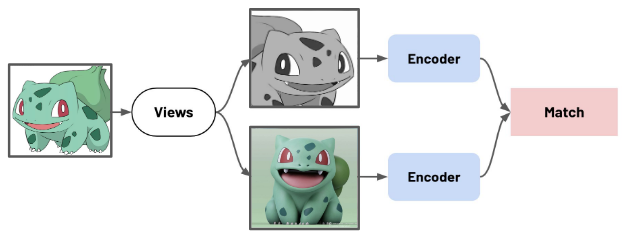
\includegraphics[width=0.6\textwidth]{images/SS22.png}
    \caption{SimCLR}
    \label{fig:MHA2}
\end{figure}

\begin{wrapfigure}{r}{0.35\textwidth}
    \centering
    \vspace{-10pt}
    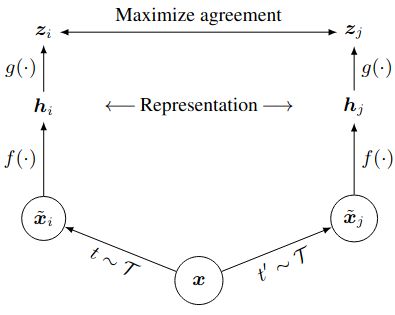
\includegraphics[width=\linewidth]{images/SS23.png}
    \label{fig:Scaled Dot Product Attention}
    \vspace{-10pt}
\end{wrapfigure}
SimCLR (Simple Framework for Contrastive Learning of Visual Representations) is a self-supervised contrastive learning framework that learns visual representations by maximizing agreement between different augmented views of the same data sample.

Given an input image $x$, two stochastic data augmentation operators $t \sim \mathcal{T}$ and $t' \sim \mathcal{T}$ are independently sampled from a family of transformations and applied to obtain two correlated views:
\[
\tilde{x}_i = t(x), \quad \tilde{x}_j = t'(x).
\]
These two views form a \textbf{positive pair}, while views obtained from different images naturally act as \textbf{negative samples}.

Each augmented image is processed by a shared \textbf{encoder network} $f(\cdot)$, producing intermediate representations:
\[
h_i = f(\tilde{x}_i), \quad h_j = f(\tilde{x}_j).
\]
The representations are then mapped by a \textbf{projection head} $g(\cdot)$, typically implemented as a multilayer perceptron, yielding the embeddings used for contrastive learning:
\[
z_i = g(h_i), \quad z_j = g(h_j).
\]

A key aspect of SimCLR is that it does \textbf{not explicitly sample negative examples}. Given a mini-batch of $N$ images, two augmented views are generated for each image, resulting in a total of $2N$ samples. For a given anchor representation, the corresponding positive sample is the other augmented view of the same image, while the remaining $2(N-1)$ augmented views in the batch act as negative samples. This explains the appearance of $2N$ terms in the contrastive loss formulation.

The similarity between two embeddings is measured using the \textbf{cosine similarity}, defined as:
\[
\text{sim}(u, v) = \frac{u^\top v}{\|u\| \, \|v\|},
\]
which focuses on the angular distance between normalized embeddings and has been shown to stabilize and improve contrastive training. 

The contrastive objective is formulated using the \textbf{InfoNCE loss} with a temperature parameter $\tau$. Given a positive pair $(i,j)$ within a batch of $2N$ augmented samples, the loss for sample $i$ is:
\[
\ell_{i,j} =
- \log
\frac{
\exp\left(\text{sim}(z_i, z_j) / \tau\right)
}{
\sum_{k=1}^{2N} \mathbb{1}_{[k \neq i]}
\exp\left(\text{sim}(z_i, z_k) / \tau\right)
},
\]
where $\mathbb{1}_{[k \neq i]}$ excludes the anchor itself from the denominator.

The final SimCLR objective is obtained by symmetrizing the loss over all positive pairs in the batch:
\[
\mathcal{L}_{\text{SimCLR}} =
\frac{1}{2N}
\sum_{i=1}^{N}
\left(
\ell_{i,j(i)} + \ell_{j(i),i}
\right).
\]

An important design choice in SimCLR is the use of the projection head $g(\cdot)$. By applying the contrastive loss in the projection space rather than directly on the encoder output $h$, the encoder $f(\cdot)$ is encouraged to preserve more general and transferable information. After pretraining, the projection head is discarded, and only the encoder $f(\cdot)$ is retained for downstream tasks.

\subsubsection{Linear Evaluation on SimCLR Features}
\begin{wrapfigure}{r}{0.45\textwidth}
    \centering
    \vspace{-10pt}
    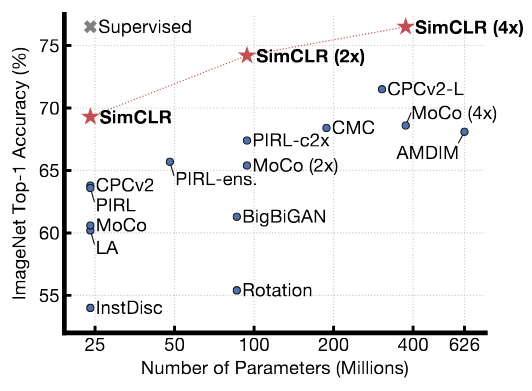
\includegraphics[width=\linewidth]{images/SS24.png}
    \label{fig:Scaled Dot Product Attention}
    \vspace{-10pt}
\end{wrapfigure}
This figure reports the performance of SimCLR representations evaluated through the \textbf{linear evaluation protocol}. The feature encoder is first pretrained on the entire ImageNet dataset using SimCLR, after which it is \textbf{frozen} and a linear classifier is trained on top using labeled data. The results show that SimCLR achieves performance comparable to, and in some cases surpassing, supervised pretraining, highlighting the quality and transferability of the learned representations.

\subsubsection{Linear Evaluation on SimCLR Features}
\begin{wrapfigure}{r}{0.45\textwidth}
    \centering
    \vspace{-10pt}
    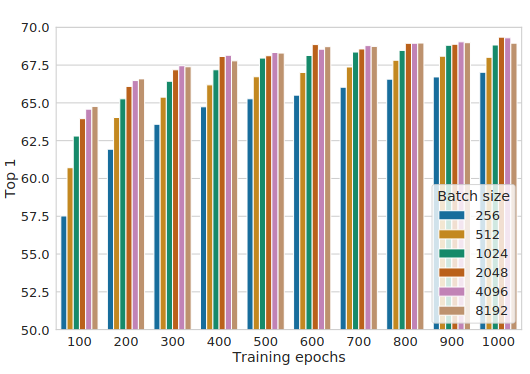
\includegraphics[width=\linewidth]{images/SS25.png}
    \label{fig:Scaled Dot Product Attention}
    \vspace{-10pt}
\end{wrapfigure}
This figure reports the performance of SimCLR representations evaluated through the \textbf{linear evaluation protocol}. The feature encoder is first pretrained on the entire ImageNet dataset using SimCLR, after which it is \textbf{frozen} and a linear classifier is trained on top using labeled data. The results show that SimCLR achieves performance comparable to, and in some cases surpassing, supervised pretraining, highlighting the quality and transferability of the learned representations.

\chapter{Transfer Learning}

\section{Introduction}
During the course we saw some problem that can affect the NNs like the \textbf{Overfitting}, that is when the performance on the training test are very high and on the test set very low, and the \textbf{Epistemic of Uncertainty} that essentially is the uncertainty on the learned model parameter caused by the lack of knowledge of the data.

The first idea that can be arise to solve this problems is use something like some \textbf{regularization techniques} or "simply" \textbf{collect more data}.

Another idea can be to inject \textbf{prior knowledge} into our model, in order to guide the
learning process toward more plausible solutions.  
The idea is to \textbf{reduce epistemic uncertainty by injecting prior knowledge into our model}.
This approach is known as \textbf{inductive bias}.

\subsection{Inductive Bias}
The \textbf{inductive bias} refers to the set of assumptions, constraints, or prior knowledge
encoded in a learning algorithm, which guide it to favor certain hypotheses over others.
When multiple explanations fit the training data equally well, the inductive bias determines
which hypothesis is preferred by the model.

Formally, the inductive bias $B$ of a learning algorithm $A$ can be defined as the set of
assumptions used to select a single hypothesis $h^*$ from all hypotheses consistent with the
training data. Let $H$ be the hypothesis space, $D$ the dataset, and $L$ a loss function:
\[
h^* = \arg\min_{h \in H} L(h, D) \quad \text{s.t. } h \in B
\]
where $B$ can be interpreted in two equivalent ways:
\begin{compactitemize}
    \item $B \subset H$: restriction of the hypothesis space (\textbf{restriction bias});
    \item $B : H \rightarrow \mathbb{R}$: preference ordering over hypotheses (\textbf{preference bias}).
\end{compactitemize}

Equivalently, an inductive bias can be seen as either a restriction on the set of admissible
hypotheses or as a preference among them.

Typical examples of inductive bias in modern neural architectures include:
\begin{compactitemize}
    \item \textbf{Convolutional Neural Networks (CNNs)}: assume that images exhibit locality
    and translation-invariant patterns, drastically reducing the hypothesis space;
    \item \textbf{Sparse Autoencoders}: enforce sparse representations, encouraging the model
    to capture meaningful and disentangled semantic features;
    \item \textbf{Graph Neural Networks (GNNs)}: exploit the adjacency matrix to encode structural
    priors about relationships and interactions in the domain.
\end{compactitemize}

\begin{infobox}[Note]
    Note that \textbf{Transformers} retain relatively weak inductive biases compared to CNNs or GNNs, delegating most structural assumptions to the data itself.
\end{infobox}

\subsection{Transfer Learning}
\textbf{Transfer Learning} is a learning paradigm in which knowledge acquired from a
\emph{source task/domain}, typically data-rich, is reused to improve performance on a related
\emph{target task/domain}, usually characterized by limited data availability.
This knowledge is encoded in the representations and parameters learned by the model during
pretraining.

More formally, transfer learning leverages representations learned on a source domain to bias
the learning process on the target domain.
For this reason, transfer learning can be interpreted as a particular and powerful form of
\textbf{inductive bias}.

The key assumption underlying transfer learning is that the optimal hypothesis for the target
task is likely to be similar to a good hypothesis for the source task.
Equivalently, pretraining on a source domain provides model parameters $\theta_S$ that are close
to an optimal solution $\theta_T^*$ for the target task.
As a consequence, the pretrained model acts as a strong prior, significantly reducing
\textbf{epistemic uncertainty} in data-scarce scenarios.

\subsection{Fine-Tuning}
\textbf{Fine-tuning} is the most common strategy used in transfer learning.
The idea is to first train a model on a large-scale source task and then reuse the learned
weights as initialization for training on the target task.

The typical fine-tuning procedure consists of the following steps:
\begin{compactitemize}
    \item pretrain a model (e.g. a CNN or a Transformer) on a source task;
    \item obtain the learned parameters from the source model;
    \item initialize the target model with these parameters;
    \item further train the model on the target task using the available data.
\end{compactitemize}

\begin{wrapfigure}{r}{0.3\textwidth}
    \centering
    \vspace{-10pt}
    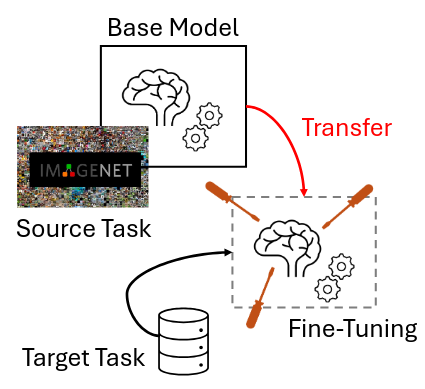
\includegraphics[width=\linewidth]{images/LT1.png}
    \label{fig:Scaled Dot Product Attention}
    \vspace{-10pt}
\end{wrapfigure}

In computer vision, a common example is pretraining a CNN on ImageNet and then fine-tuning it
for a specific task such as medical image classification.
In natural language processing, language models are often pretrained on large text corpora
(e.g. Wikipedia) and fine-tuned for downstream tasks such as sentiment analysis.

By starting from pretrained weights instead of random initialization, fine-tuning encourages
the model to exploit features that capture general and transferable patterns
(e.g. edges, textures, shapes, or semantic structures), improving generalization and reducing
the amount of data required for effective learning.

\section{Fine-Tuning}
We have seen that today the typical way to train a NN is using a fine-tuning approach, this beacuse lead to many advantage. This advantage including:
\begin{compactitemize}
    \item \textbf{Performance}: fine tuning often \textbf{outperforms} training from scratch, especially in data-scarce scenarios.
    \item \textbf{Computational constraints}: few companies can afford to train very large models from scratch.
    \item \textbf{Data availability}: large-scale dataset required for training from scratch are not always accessible.
\end{compactitemize}

\subsection{The effectiveness of Fine-Tuning}
\begin{figure}[H]
    \centering
    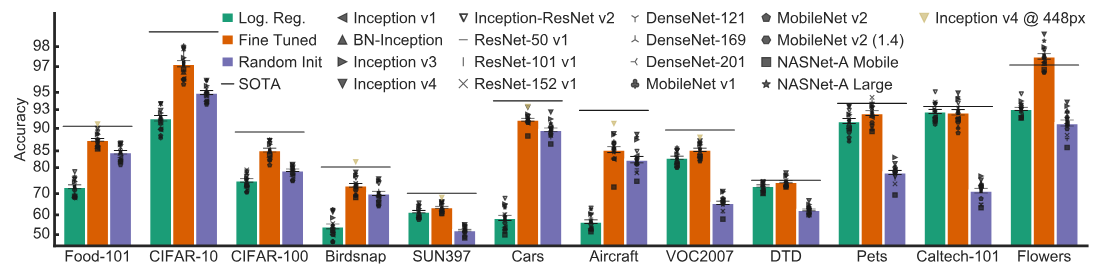
\includegraphics[width=0.9\textwidth]{images/LT2.png}
    \caption{Image from "Do better ImageNet model transfer better"}
    \label{fig:MHA2}
\end{figure}
The figure illustrates the effectiveness of \textbf{fine-tuning} compared to other strategies
for reusing or training vision models.

The horizontal axis reports several image classification datasets (Food-101, CIFAR-10,
CIFAR-100, Birdsnap, SUN397, Cars, Aircraft, VOC2007, DTD, Pets, Caltech-101, Flowers), while the
vertical axis shows the classification \textbf{accuracy}.

For each dataset, three bars are displayed:
\begin{compactitemize}
    \item \textbf{green}: logistic regression, where only the final classifier is trained on
    the target dataset and the pretrained network is used as a fixed feature extractor;
    \item \textbf{orange}: fine-tuning, where the entire pretrained network is further trained
    on the target dataset;
    \item \textbf{purple}: training from random initialization, with no transfer of knowledge.
\end{compactitemize}

The bars represent the mean accuracy across multiple architectures (e.g. Inception, ResNet,
DenseNet, MobileNet, NASNet), indicated by the black markers above each bar, while the vertical
error bars denote the standard error. The horizontal black lines correspond to the previous
state-of-the-art (SOTA) results on each dataset.

Overall, the figure shows that, for most datasets, fine-tuning pretrained models achieves
higher accuracy than both logistic regression and training from scratch, often matching or
surpassing the existing SOTA, highlighting the effectiveness of knowledge transfer from
ImageNet.

\subsection{Fine-Tuning in the Low-Data Regime}
\begin{figure}[H]
    \centering
    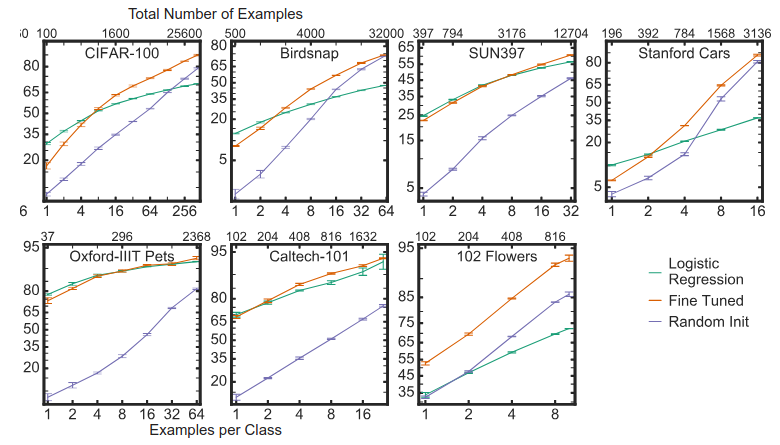
\includegraphics[width=0.8\textwidth]{images/LT3.png}
    \caption{Image from "Do better ImageNet model transfer better"}
    \label{fig:MHA2}
\end{figure}
This image analyzes the behavior of fine-tuning in scenarios where only a small number of
training examples per class are available.
The curves compare logistic regression, fine-tuning, and training from random initialization
as the number of samples increases.

The results show that pretraining on ImageNet provides a significant advantage when data is
scarce, especially for fine-grained recognition tasks.
In the low-data regime, fine-tuning consistently outperforms both logistic regression and
random initialization, highlighting the strong prior induced by pretrained representations.
As the dataset size grows, the performance gap gradually narrows, since models trained from
scratch can eventually learn suitable representations.

\subsection{Fine-Tuning and Faster Convergence}
\begin{figure}[H]
    \centering
    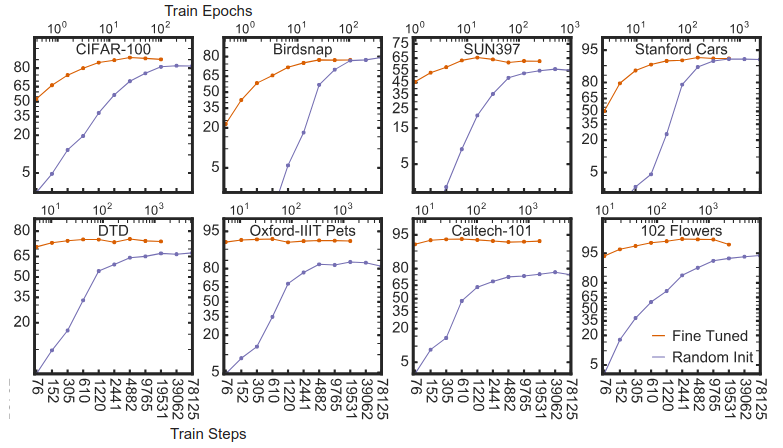
\includegraphics[width=0.8\textwidth]{images/LT4.png}
    \caption{Image from "Do better ImageNet model transfer better"}
    \label{fig:MHA2}
\end{figure}
This image illustrates the effect of fine-tuning on training dynamics by comparing convergence
speed.
Models pretrained on ImageNet are contrasted with models trained from random initialization
as a function of training steps.

The plots show that pretrained networks converge much faster, reaching high accuracy in far
fewer training iterations.
Even when the final accuracy achieved by both approaches is similar, fine-tuning offers a
clear optimization advantage by starting from parameters that are already close to a good
solution.
This faster convergence reduces training time and computational cost, further motivating the
use of transfer learning in practice.

\subsection{Why Has Fine-Tuning Become So Dominant?}
\begin{wrapfigure}{r}{0.2\textwidth}
    \centering
    \vspace{-10pt}
    
\includegraphics[width=\linewidth]{images/LT5.png}
    \label{fig:Scaled Dot Product Attention}
    \vspace{-10pt}
\end{wrapfigure}
Fine-tuning has become the dominant paradigm in modern deep learning due to a combination of
practical and computational advantages.

First, it enables extensive \textbf{reuse}. Modern frameworks and libraries provide access to
large collections of pretrained models whose weights can be easily adapted to new tasks with
minimal additional training. This avoids the massive computational cost required for training
large models from scratch and significantly reduces the time-to-market when deploying machine
learning solutions.

Second, fine-tuning leads to a reduced \textbf{design effort}. Pretrained models are typically
associated with well-tested architectures, including carefully chosen layers, activation
functions, and hyperparameters. These design choices have been validated by extensive research
and benchmarking, allowing practitioners to focus on the specifics of the target problem rather
than on architectural exploration or low-level model tuning.

\subsection{Technical Aspects of Fine-Tuning}
One of the key technical decisions in fine-tuning concerns whether to \textbf{freeze some layers}
of the pretrained network. Earlier layers typically capture generic, low-level features such as
edges, textures, and simple patterns, which are often transferable across different tasks.
For this reason, these layers can be reused and kept fixed during fine-tuning, while higher
layers are adapted to the target task.

Freezing layers provides several advantages:
\begin{compactitemize}
    \item \textbf{Reduced computation}: frozen layers can be set to \texttt{no\_grad}, lowering
    memory usage and eliminating gradient-related FLOPs;
    \item \textbf{Faster convergence}: the optimizer focuses only on adapting task-specific
    layers, requiring fewer parameter updates, which speeds up training;
    \item \textbf{Stability}: freezing early layers helps prevent the degradation of useful
    generic representations learned on the source task;
    \item \textbf{Preserved generalization}: early layers encode low-level, task-agnostic features
    such as edges, textures, and simple visual patterns that generalize well across domains.
    Keeping these layers fixed preserves the inductive bias learned on the source task and acts
    as a form of regularization, reducing the risk of overfitting when the target dataset is
    small and leading to more consistent and reliable performance.
\end{compactitemize}

\begin{figure}[H]
    \centering
    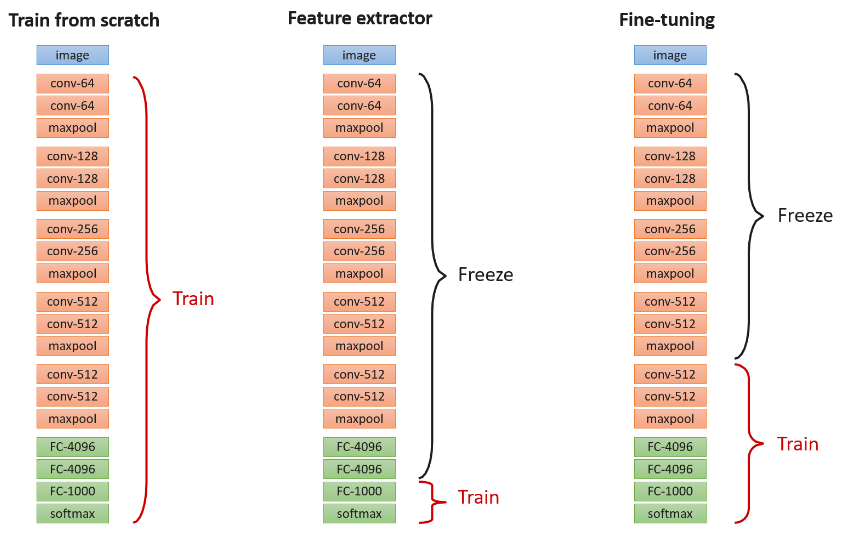
\includegraphics[width=0.8\textwidth]{images/LT6.png}
    \label{fig:MHA2}
\end{figure}


Different fine-tuning strategies can be adopted depending on how many layers are trained:
\begin{compactitemize}
    \item \textbf{Last layer only}: only the classifier is trained. This approach enables very
    fast adaptation with a low risk of overfitting, but offers limited flexibility. It is also
    known as \textbf{linear probing};
    \item \textbf{Last $N$ layers}: strikes a balance between adaptation capacity and overfitting
    risk by allowing partial modification of the pretrained representation;
    \item \textbf{All layers}: the entire network is fine-tuned, providing maximum flexibility at
    the cost of higher computational requirements and an increased risk of overfitting.
\end{compactitemize}

\begin{figure}[H]
    \centering
    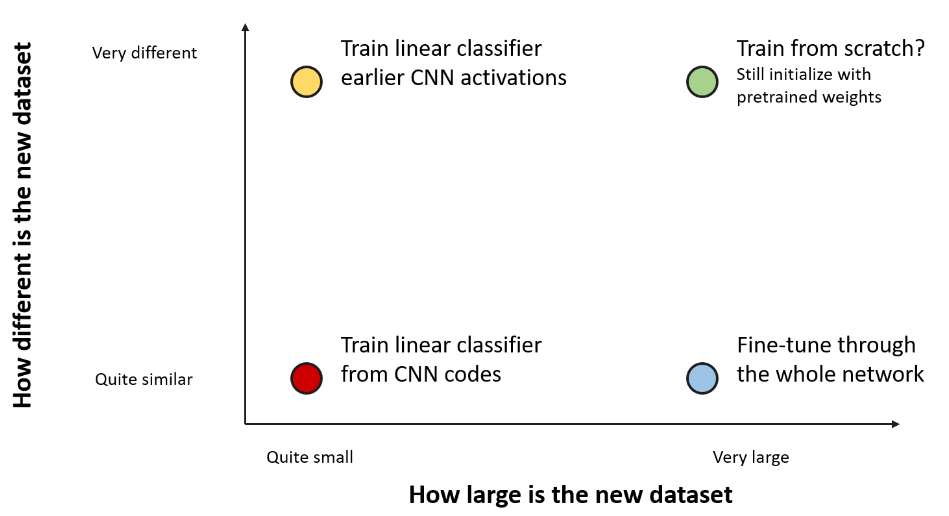
\includegraphics[width=0.7
    \textwidth]{images/LT7.png}
    \label{fig:MHA2}
\end{figure}

\begin{infobox}[Note]
    Note that linear probing is often used in the literature as a quick diagnostic tool to evaluate
the quality and transferability of features produced by a frozen backbone on downstream tasks.
\end{infobox}

\subsection{Learning Rate Strategies during Fine-Tuning}
The choice of the learning rate and its scheduling plays a crucial role in effective fine-tuning,
as pretrained networks are sensitive to large parameter updates that may destroy useful
representations learned on the source task.

A simple approach is to use a \textbf{uniform learning rate}, where the same learning rate is
applied to all trainable layers. This strategy is easy to implement and works reasonably well
in practice, but it can be suboptimal: early layers may be over-updated, damaging generic
features, or under-updated, limiting adaptation.

A more effective strategy is to adopt \textbf{layer-specific learning rates}, assigning larger
learning rates to the last, task-specific layers and smaller ones to earlier layers. This
encourages rapid adaptation of high-level features while preserving low-level, transferable
representations. This technique is also known as the \textbf{Slow Learner} approach.

Finally, \textbf{learning rate warmup schedules} are often used during fine-tuning, especially
when updating all layers. The idea is to gradually increase the learning rate during the initial
training iterations, preventing sudden large updates that could destabilize pretrained weights
and lead to poor convergence. Essentially we wait until the NN is comfortable with the new data.

\subsection{An Alternative: LP-FT}
\begin{wrapfigure}{r}{0.6\textwidth}
    \centering
    \vspace{-10pt}
    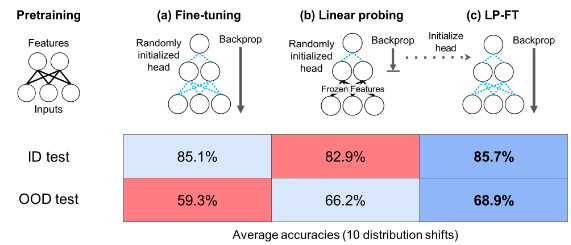
\includegraphics[width=\linewidth]{images/LT8.png}
    \label{fig:Scaled Dot Product Attention}
    \vspace{-10pt}
\end{wrapfigure}
Standard fine-tuning, while effective on in-distribution (ID) data, can sometimes distort
pretrained features, leading to degraded performance when the model is evaluated on
out-of-distribution (OOD) data. This issue becomes particularly relevant under large
distribution shifts, where aggressive parameter updates may harm previously learned
transferable representations.

To address this problem, has been propose proposes the \textbf{LP-FT} strategy
(\textit{Linear Probing + Fine-Tuning}), which combines the strengths of linear probing and
fine-tuning in a two-stage procedure:
\begin{enumerate}
    \item \textbf{Linear probing}: the pretrained backbone is frozen and only a linear
    classification head is trained on the target task. This step adapts the classifier to the
    pretrained feature space without modifying the feature extractor.
    \item \textbf{Fine-tuning}: starting from the adapted classifier, the entire network is
    fine-tuned end-to-end on the target data.
\end{enumerate}

The intuition behind LP-FT is that linear probing provides a well-aligned initialization for the
task-specific head, reducing harmful gradients flowing into the backbone during subsequent
fine-tuning. As a result, the pretrained features are better preserved, leading to improved
generalization.

Another explanation for the effectiveness of this method is that, once linear probing is
completed and the classification head is properly trained, the head guides the subsequent
updates of the backbone during fine-tuning.
As a result, the gradients reaching the backbone are smaller, more stable, and more
task-targeted.

This mechanism helps prevent excessive distortion of pretrained features, allowing the model
to adapt to the target task while preserving the useful representations learned on the source
domain.
Empirical results show that LP-FT achieves higher accuracy than standard fine-tuning both on
ID data and under various OOD shifts, confirming that initializing fine-tuning with a probed
head can mitigate feature distortion and enhance robustness.

\subsection{Batch Normalization in Fine-Tuning}
During fine-tuning, Batch Normalization (BN) layers require special attention.
In some settings, even when the network weights are kept frozen, the \textbf{BatchNorm
statistics} are updated to better match the target domain.
In particular:
\begin{compactitemize}
    \item only the \textbf{running mean} and \textbf{running variance} of the BatchNorm layers are
    updated;
    \item the learnable parameters $\gamma$ (scale) and $\beta$ (shift) can either be kept fixed
    or allowed to update, depending on the fine-tuning strategy.
\end{compactitemize}

Updating only the BN statistics is equivalent to running one training epoch with SGD and
learning rate set to zero: model weights do not change, but normalization statistics gradually
adapt to the target data distribution.

The intuition behind this approach is that it allows the model to \textbf{align feature
normalization to the target domain} without altering the learned representations themselves.
This can significantly reduce distribution mismatch between source and target domains.

For this reason, BN statistics adaptation is widely used in \textbf{domain adaptation} settings,
where the goal is to improve generalization across different data distributions while
minimizing changes to the pretrained model.

\subsection{Limitations of Fine-Tuning}
Some limitations of fini tuning are:
\begin{compactitemize}
    \item \textbf{Architectural rigidity}: Inherits the architecture of the pretrained model, which may not be optimal for the new task (e.g. too many layers -> computational overhead)
    \item \textbf{Dependence on external data/models}: Requires access to pretrained models and their associated datasets, including potential licensing or usage restrictions.
    \item \textbf{Inherited biases}: Any biases present in the source dataset can be transferred and potentially amplified in the target task.
\end{compactitemize}

\begin{figure}[H]
    \centering
    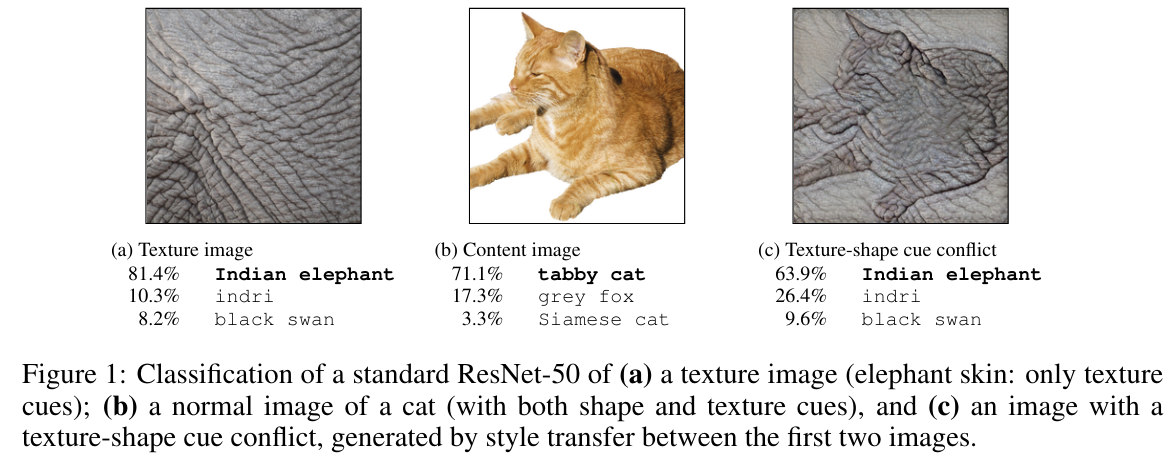
\includegraphics[width=0.9
    \textwidth]{images/LT9.png}
    \label{fig:MHA2}
\end{figure}
\begin{figure}[H]
    \centering
    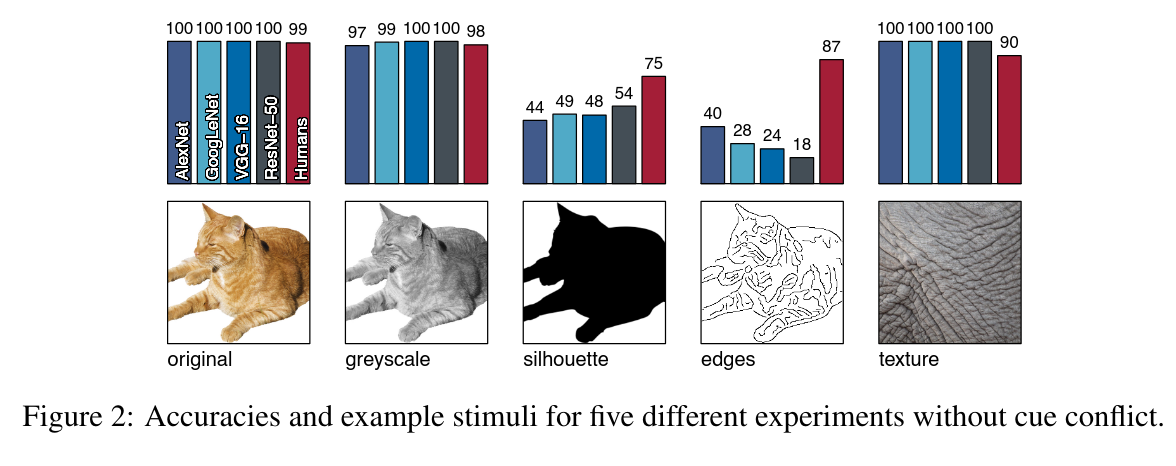
\includegraphics[width=0.9
    \textwidth]{images/LT10.png}
    \label{fig:MHA2}
\end{figure}

The figure shows that a standard ResNet relies predominantly on \textbf{texture cues} rather than
on object shape when performing image classification. In the presence of a texture–shape
conflict, the network tends to predict the class suggested by the texture, revealing a strong
texture bias.

This experiment further confirms that ImageNet-trained ResNet models inherit a
\textbf{bias toward texture-based features}. Even when shape information is preserved or
isolated, classification accuracy remains high only when texture information is available,
highlighting the limited role of global shape in the learned representations.

\subsubsection{Model Storage}
A major limitation of standard fine-tuning is its \textbf{large storage requirement}.
Fine-tuning updates the entire set of model parameters, which implies that a separate copy of
the full model must be stored for each downstream task.

For large models, such as large language models with billions of parameters, this results in a
significant memory and disk footprint per task.
Maintaining multiple fine-tuned versions of the same base model becomes costly and inefficient,
especially when deploying systems at scale.

Additionally, this approach is inflexible in resource-constrained settings, where switching
between tasks may require loading different large model checkpoints, incurring high latency
and memory overhead.

To address these limitations, more recent approaches focus on
\textbf{Parameter-Efficient Fine-Tuning (PEFT)}, such as LoRA, adapters, and prefix-tuning, which
enable task adaptation while drastically reducing storage and memory costs.

\section{Teacher-Student approaches}

\subsection{Deep Ensembles and Impact of Depth}
\begin{wrapfigure}{r}{0.5\textwidth}
    \centering
    \vspace{-10pt}
    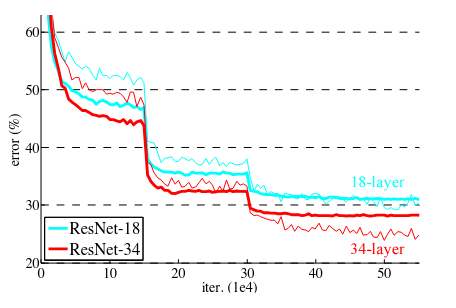
\includegraphics[width=\linewidth]{images/LT11.png}
    \label{fig:Scaled Dot Product Attention}
    \vspace{-10pt}
\end{wrapfigure}
It is well known that increasing the depth of a neural network enables the model to learn more
complex patterns and richer hierarchical representations, often leading to improved
performance compared to smaller models.

Similarly, \textbf{deep ensembles}, where multiple models are trained independently and converge
to different local minima, typically achieve stronger performance and improved robustness with
respect to single models.

These two approaches share important similarities:
\begin{compactitemize}
    \item both rely on \textbf{redundancy of representations} to improve accuracy and robustness;
    \item both generally achieve \textbf{very strong results} across a wide range of tasks.
\end{compactitemize}

Despite their effectiveness, both deeper models and ensemble methods present a major drawback:
they are often \textbf{hard to deploy in production} due to high computational and memory
requirements.
In practical scenarios, especially at test time, it is crucial to minimize computational cost
and memory footprint, as these constraints are typically much more severe during inference than
during training.

\subsection{The Insects Parallelism}

The insects parallelism provides an intuitive analogy for understanding modern large-scale
machine learning systems and their lifecycle.

Many insects have two very different stages. In the \textbf{larval stage}, the organism is
optimized for extracting energy and nutrients from the environment. This stage is slow,
resource-intensive, but extremely effective at growth.  
Similarly, during the \textbf{training stage} in machine learning, large and complex models
— often deep, redundant, and heavily regularized — are used to extract structure and knowledge
from massive datasets. At this stage, efficiency is not the primary concern.

In contrast, the \textbf{adult stage} (the butterfly) is optimized for mobility and survival,
operating efficiently with limited resources.  
This mirrors the \textbf{deployment stage} of machine learning models, where systems must
perform inference in real time, at scale, and under strict computational and memory constraints.

\begin{figure}[H]
    \centering
    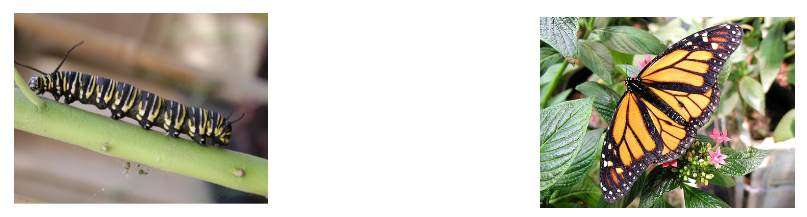
\includegraphics[width=0.9\textwidth]
    {images/LT12.png}
    \label{fig:MHA2}
\end{figure}

The key insight of this perspective is that \textbf{learning and deployment have different
requirements}. A large and complex model is ideal for learning, but not for deployment.
Therefore, the goal is to first train a powerful \emph{larval} model to simplify learning, and
then transfer the acquired knowledge into a smaller and more efficient \emph{butterfly} model
that is suitable for real-world use.

In this view, ensembles or large models are treated as a function mapping inputs to outputs.
Once this function is learned, the internal structure and parameterization of the model become
secondary.  
The central question then becomes: \emph{can we transfer the knowledge stored in this function
into a single, smaller model?}
This question naturally leads to techniques such as \textbf{knowledge distillation}, which aim
to bridge the gap between powerful learners and efficient deployable models.

\subsection{Knowledge Distillation}
\begin{wrapfigure}{r}{0.4\textwidth}
    \centering
    \vspace{-10pt}
    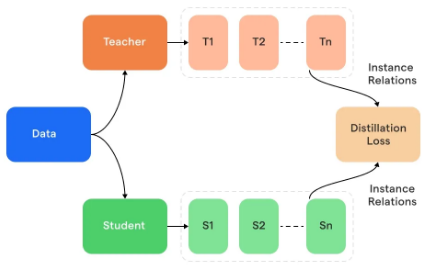
\includegraphics[width=\linewidth]{images/LT13.png}
    \label{fig:Scaled Dot Product Attention}
    \vspace{-10pt}
\end{wrapfigure}
\textbf{Knowledge Distillation (KD)} is a technique designed to transfer knowledge from a large,
complex model (the \textbf{teacher}) to a smaller and more efficient model (the \textbf{student}).
The main idea is to train the student not only using ground-truth labels, but also to mimic the
output distribution produced by the teacher.

\newpage
The teacher model can be:
\begin{compactitemize}
    \item a single, large and cumbersome model (e.g. deeper or wider architecture);
    \item an ensemble of multiple models, whose predictions are averaged to obtain more reliable
    outputs.
\end{compactitemize}

\subsubsection{Softened Probabilities}
\begin{wrapfigure}{r}{0.5\textwidth}
    \centering
    \vspace{-10pt}
    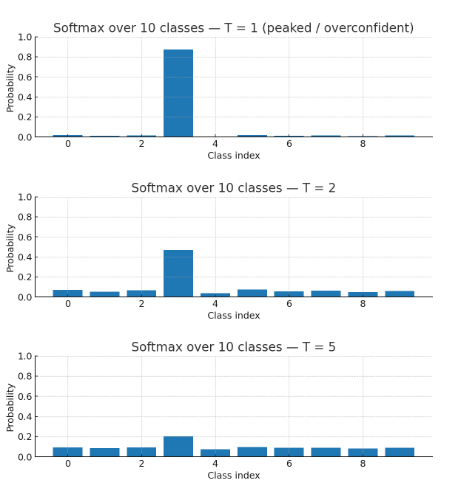
\includegraphics[width=\linewidth]{images/LT14.png}
    \label{fig:Scaled Dot Product Attention}
    \vspace{-10pt}
\end{wrapfigure}
During distillation, the teacher produces logits $z_i$ for each class $i$.
Instead of applying the standard softmax, a \textbf{temperature-scaled softmax} is used:
\[
p_i^{(T)} = \frac{\exp(z_i / T)}{\sum_j \exp(z_j / T)}, \qquad T > 1
\]
A higher temperature $T$ produces a \textbf{softer probability distribution}, characterized by:
\begin{compactitemize}
    \item lower confidence in the top predicted class;
    \item higher probability mass assigned to classes considered similar by the teacher.
\end{compactitemize}
At inference time, the temperature is set back to $T = 1$.

These softened probabilities encode what is often called \textbf{dark knowledge}, i.e. information
about inter-class similarities that is not present in one-hot labels.

\subsubsection{Training Procedure}
The distillation process follows a two-model training loop:
\begin{enumerate}
    \item perform a forward pass with the teacher to compute teacher logits $z_t$;
    \item perform a forward pass with the student to compute student logits $z_s$;
    \item update the student parameters by minimizing a mixed loss function:
\end{enumerate}

\[
\mathcal{L}_{\text{student}} =
\alpha \, \mathcal{L}_{\text{CE}}(y, \sigma(z_s))
+ (1 - \alpha) \, T^2 \, \mathcal{L}_{\text{CE}}\big(\sigma(z_t/T), \sigma(z_s/T)\big)
\]

where:
\begin{compactitemize}
    \item $y$ is the ground-truth one-hot label;
    \item $\sigma(\cdot)$ denotes the softmax function;
    \item $T$ is the distillation temperature;
    \item $\alpha$ balances hard targets and soft targets.
\end{compactitemize}

\subsubsection{Effectiveness of Knowledge Distillation}
Empirically, incorporating soft targets during training typically improves performance compared
to using hard labels alone, often yielding:
\[
\text{KD} \; > \; \text{Student trained from scratch}
\]

Experimental results on CIFAR-100 confirm that distillation consistently improves student
accuracy, even when teacher and student architectures differ. This demonstrates that the
knowledge transferred through softened outputs is not tightly coupled to a specific
architecture, but captures more general and transferable patterns learned by the teacher.

\subsection{Dark Knowledge}
\textbf{Dark knowledge} refers to the information contained in the relative probabilities
assigned by a model to the \textbf{non-argmax classes}, also known as secondary information.
Unlike one-hot labels, which provide supervision only for the correct class, dark knowledge
encodes the similarity structure between classes learned by the teacher model.

For example, given an image of a cat, a teacher model may produce an output distribution such as:
\[
[\text{Cat}: 0.65,\; \text{Dog}: 0.25,\; \text{Fox}: 0.07]
\]
This distribution reveals that the teacher considers dogs more similar to cats than foxes, an
insight that is completely lost when using hard one-hot targets.

These secondary probabilities guide the student to learn \textbf{richer and smoother decision
boundaries} than those induced by standard supervision alone. In particular, each training
example provides constraints on multiple class relationships, rather than enforcing a single,
hard decision.

As a result, soft targets act as a \textbf{powerful regularizer}, discouraging overconfident
predictions and improving generalization. This regularization effect is a key reason why
knowledge distillation often leads to better performance and more robust models.

\subsection{Distillation via Pre-Softmax Activations}
An alternative approach to standard knowledge distillation goes beyond probability matching.
Instead of aligning the softened output probabilities of teacher and student, it directly
matches their \textbf{pre-softmax activations} (logits).

Let $z_t$ and $z_s$ denote the logits produced by the teacher and the student, respectively.
Logit-based distillation minimizes the Mean Squared Error (MSE) between them:
\[
\mathcal{L}_{\text{logit}} = \frac{1}{K} \sum_{i=1}^{K} (z_{t,i} - z_{s,i})^2
\]
where $K$ is the number of classes.

This loss can be combined with the standard cross-entropy loss computed using the true labels,
allowing the student to learn both from ground-truth supervision and from the teacher’s
internal representations.

One key advantage of logit-based distillation is that it avoids potential information loss
introduced by the softmax transformation, which can compress or obscure differences between
classes. By operating directly on logits, the method emphasizes the transfer of secondary
information related to class similarities and relative confidence levels learned by the
teacher, leading to more faithful knowledge transfer.

\subsection{Applications of Knowledge Distillation}
Knowledge distillation is a versatile technique with wide applicability across different stages
of model development and deployment.

A primary application is \textbf{model compression}. By distilling knowledge from a large
teacher into a smaller student, it is possible to significantly reduce memory footprint and
computational cost, enabling deployment on edge devices and mobile platforms.

Closely related is \textbf{latency reduction}. Distilled models are typically faster at
inference time, making them suitable for real-time applications such as speech recognition,
video analytics, and online recommendation systems.

Another common use case is \textbf{ensemble-to-single transfer}. Instead of deploying a large
and expensive ensemble of models, knowledge distillation allows transferring most of the
ensemble’s accuracy into a single compact model, greatly simplifying deployment.

Knowledge distillation is also effective for \textbf{cross-architecture transfer}. For example,
knowledge can be distilled from a CNN to a Transformer, or vice versa, allowing the student to
benefit from the strengths of a different architectural family.

In \textbf{domain adaptation} settings, a teacher trained on one domain can guide a student
operating on a related but different domain, helping reduce distribution mismatch and improve
generalization.

Finally, distillation can act as a form of \textbf{regularization during training}. In
self-distillation, a model is trained to match its own earlier predictions, which encourages
consistency and often leads to improved generalization even without an external teacher.

\subsection{Similarity-Preserving Knowledge Distillation}
\begin{wrapfigure}{r}{0.5\textwidth}
    \centering
    \vspace{-10pt}
    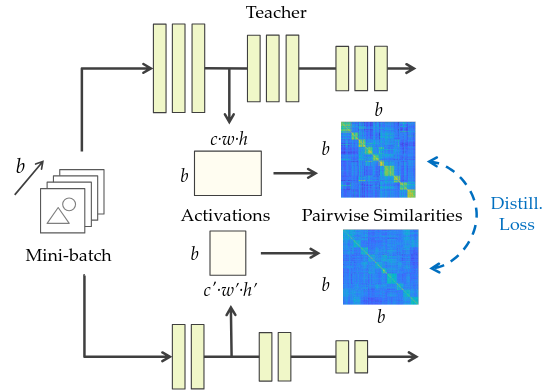
\includegraphics[width=\linewidth]{images/LT15.png}
    \label{fig:Scaled Dot Product Attention}
    \vspace{-10pt}
\end{wrapfigure}
Similarity-Preserving Knowledge Distillation is an extension of standard knowledge distillation
that aims to transfer not only the output predictions of a teacher model, but also the
\textbf{relational structure} of the data learned in its feature space.

The key motivation is that the relationships between samples in the embedding space contain rich
semantic information that goes beyond individual class predictions. Semantically similar inputs
tend to produce similar activation patterns in a well-trained network, and preserving these
relationships can significantly improve knowledge transfer.

In this approach, feature representations are extracted from both the teacher and the student,
and pairwise similarity matrices are computed:
\begin{compactitemize}
    \item $S_T$: similarity matrix between samples in the teacher feature space;
    \item $S_S$: similarity matrix between samples in the student feature space.
\end{compactitemize}

In addition to the standard cross-entropy or distillation loss, the student is trained by
minimizing a similarity-preserving loss of the form:
\[
\mathcal{L}_{\text{SP}} = \lVert S_T - S_S \rVert_F^2
\]
where $\lVert \cdot \rVert_F$ denotes the Frobenius norm.

By aligning the similarity structure of the student with that of the teacher, this method
encourages the student to capture the same geometric organization of the data in the embedding
space. As a result, the student inherits a deeper form of knowledge that reflects how the
teacher organizes and disentangles data, leading to improved generalization and more robust
representations.

\subsection{Paying More Attention to Attention}

Attention Transfer (AT) is a knowledge distillation technique that focuses on transferring the
\textbf{spatial attention maps} from a teacher to a student model. Instead of matching full
feature maps—which may differ in dimensionality or structure—AT encourages the student to
replicate the teacher’s attention, i.e., the regions of the input that the teacher considers most
informative.
\begin{wrapfigure}{r}{0.3\textwidth}
    \centering
    \vspace{-10pt}
    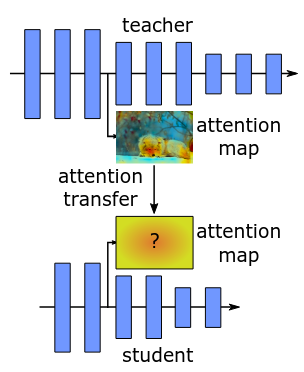
\includegraphics[width=\linewidth]{images/LT16.png}
    \label{fig:Scaled Dot Product Attention}
    \vspace{-10pt}
\end{wrapfigure}
The intuition is straightforward: attention maps highlight \textbf{where} the model focuses
during prediction. By imitating the teacher’s attention patterns, the student learns not only
\emph{what} to predict, but also \emph{where to look}. This improves knowledge transfer, even
when teacher and student differ significantly in architecture or depth.

To compute attention maps, consider feature maps $F \in \mathbb{R}^{C \times H \times W}$, where
$C$ is the number of channels. The spatial attention map is obtained by aggregating across
channels:
\[
A = \frac{1}{C} \sum_{c=1}^{C} |F_c|^p,
\qquad p \in \{1, 2\}
\]

Each attention map is then normalized to unit norm:
\[
\hat{A} = \frac{A}{\lVert A \rVert_2}
\]

Attention transfer is performed by minimizing the squared distance between the normalized
attention maps of teacher and student:
\[
\mathcal{L}_{AT} = \lVert \hat{A}_T - \hat{A}_S \rVert_2^2
\]

This loss is typically combined with standard cross-entropy or knowledge-distillation losses.
By guiding the student to mimic the teacher’s attention behavior, AT helps the student learn
more effective and interpretable feature representations, improving generalization and
transferability.

\begin{figure}[H]
    \centering
    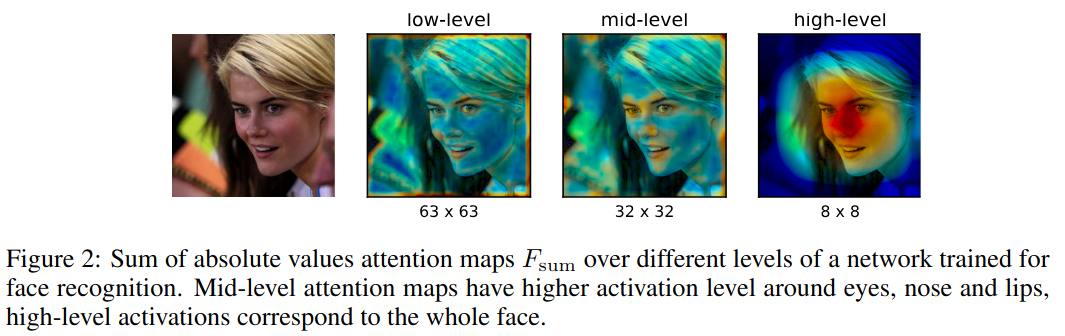
\includegraphics[width=0.9
    \textwidth]{images/LT17.png}
    \label{fig:MHA2}
\end{figure}

\subsection{FitNets: Hints for Thin Deep Networks}
FitNets extend standard knowledge distillation by transferring \textbf{intermediate feature
representations} from the teacher to the student, rather than relying only on the final output
logits. This is particularly useful when the student network is very deep but thin, a setting
in which training from scratch can be difficult and unstable.
\begin{wrapfigure}{r}{0.6\textwidth}
    \centering
    \vspace{-10pt}
    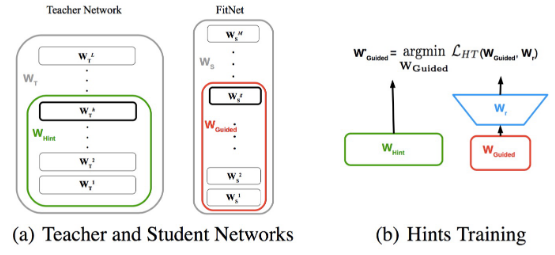
\includegraphics[width=\linewidth]{images/LT18.png}
    \label{fig:Scaled Dot Product Attention}
    \vspace{-10pt}
\end{wrapfigure}
The key motivation behind FitNets is that providing intermediate \emph{hints} from the teacher
helps guide the optimization of the student, easing the learning of meaningful representations
layer by layer instead of only through end-task supervision.

The method works as follows:
\begin{compactitemize}
    \item a \textbf{hint layer} is selected in the teacher network, typically a deep intermediate
    layer containing rich semantic information;
    \item a corresponding \textbf{guided layer} is selected in the student network, usually at a
    similar depth;
    \item if the feature dimensions do not match, a small \textbf{regressor} (e.g., a $1\times1$
    convolution or an MLP) is applied to map the student features into the teacher’s feature
    space.
\end{compactitemize}

In addition to the standard knowledge distillation or cross-entropy loss on the outputs,
FitNets minimize a hint-based loss defined as:
\[
\mathcal{L}_{\text{hint}} = \lVert r(f_S) - f_T \rVert_2^2
\]
where $f_S$ and $f_T$ denote the student and teacher feature representations at the guided and
hint layers, and $r(\cdot)$ is the regressor.

There are no strict rules for choosing hint and guided layers; the selection depends on the
architecture. In practice, choosing layers at comparable depths is a common and effective
strategy.

A key advantage of FitNets is their flexibility. They are not limited to teacher–student pairs
with similar depth or width and can be applied when:
\begin{compactitemize}
    \item the student is deeper but thinner than the teacher;
    \item the student is shallower or has a different architecture;
    \item the teacher and student have different hidden layer sizes.
\end{compactitemize}

This flexibility makes FitNets a powerful distillation technique for training compact yet deep
models while preserving much of the representational power of larger networks.

\subsection{Self-Knowledge Distillation}
\textbf{Self-Knowledge Distillation (Self-KD)} applies the distillation paradigm to two networks
that share the \textbf{same architecture}. In this case, the difference between teacher and
student does not lie in model capacity, but in the \textbf{information content of the inputs}
they receive.

In a typical setup:
\begin{compactitemize}
    \item the \textbf{teacher} is trained using richer or more informative inputs (e.g., multiple
    modalities, full-resolution data, or clean signals);
    \item the \textbf{student} is trained using degraded, partial, or noisier versions of the
    same inputs.
\end{compactitemize}

During training, a distillation loss encourages the student to match the teacher’s intermediate
feature representations or final output predictions, despite having access to less information.

The main benefit of Self-KD is that it shifts the learning challenge from \textbf{model capacity}
to \textbf{input efficiency}. Rather than relying on a larger or more complex architecture, the
student learns to extract more informative and discriminative patterns from limited data.

Interestingly, in some scenarios the student can even \textbf{surpass the teacher}, as the
distillation process acts as a strong regularizer and promotes more robust representations.

Self-KD is particularly useful in real-world settings involving \textbf{missing modalities},
partial observations, or low-quality inputs, where models must operate effectively under
information constraints.

\subsection{Applications to Video Recognition}
Self-Knowledge Distillation can be effectively applied to \textbf{video recognition} tasks such
as object tracking and video-based person re-identification, where temporal information plays a
crucial role.

In this setting, both the teacher and the student share the same network architecture (e.g.,
ResNet-50), but differ in the number of input frames they process. The \textbf{teacher} is trained
using a larger and more informative set of video frames, while the \textbf{student} is trained
using fewer frames, thus receiving limited temporal context.

The distillation loss encourages the student to match the teacher’s feature representations or
final predictions, forcing it to exploit richer temporal and spatial cues from reduced visual
evidence. Through this process, the student learns to compactly encode motion and appearance
information that would otherwise require longer sequences.

\begin{wrapfigure}{r}{0.7\textwidth}
    \centering
    \vspace{-10pt}
    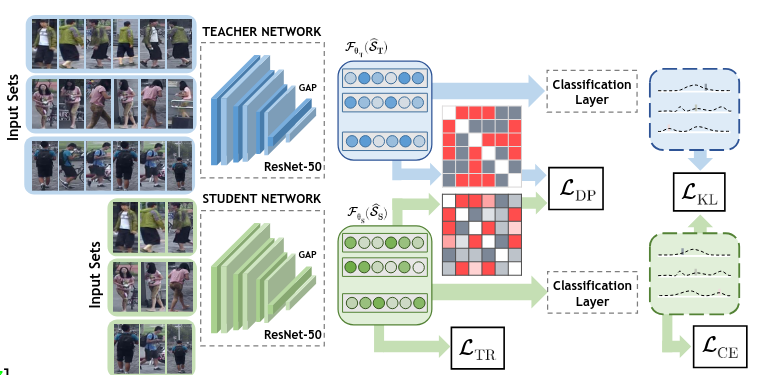
\includegraphics[width=\linewidth]{images/LT19.png}
    \label{fig:Scaled Dot Product Attention}
    \vspace{-10pt}
\end{wrapfigure}

This approach allows the deployment of video recognition models with lower computational cost
and latency, while retaining competitive performance. As a result, Self-KD is particularly
well-suited for real-time video applications where memory, bandwidth, or frame availability are
limited.

\chapter{Parameter Efficient Fine-Tuning}
\chapter{Continual Learning}

\section{Introduction}

\subsection{Humans and Memory}
Human intelligence is characterized by its remarkable ability to learn from sequences of events and tasks without erasing prior compe-
tencies. A person may first learn to distinguish cats from dogs, and later learn to distinguish cars from boats, while still retaining the
ability to correctly identify a dog. \textbf{This sequence learning capability} is central to human cognition: new knowledge is integrated without
completely overwriting what came before

\begin{figure}[H]
    \centering
    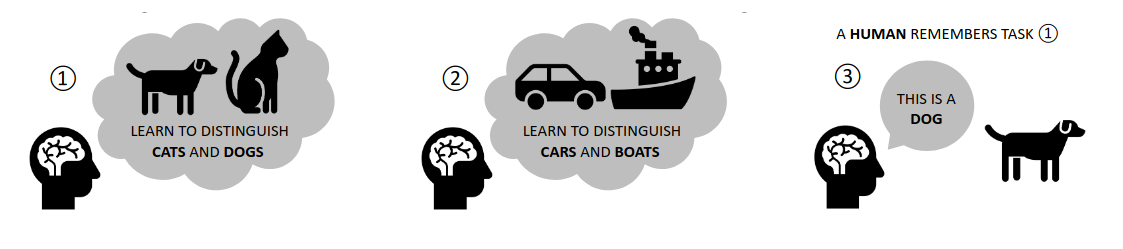
\includegraphics[width=0.75
    \textwidth]{images/CL1.png}
    \label{fig:MHA2}
\end{figure}

\subsection{Neural Networks and Catastrophic Forgetting}
Artificial Neural Networks behave differently. When trained on tasks sequentially, they tend to forget earlier ones: a phenomenon
known as \textbf{catastrophic forgetting}. After learning Task 1 (cats vs. dogs) and then Task 2 (cars vs. boats), a neural network may incorrectly
classify a dog as a car. Performance on the most recent task is preserved, while accuracy on previous tasks sharply deteriorates. This
happens because networks show an \textbf{intrinsic bias toward recently learned tasks}, making them less versatile in long-term, incremental
learning scenarios.

This issue is closely connected to our earlier discussions about \textbf{PEFT (Parameter-Efficient Fine-Tuning)}. When performing \textbf{full fine-tuning
(FFT)}, we adjust all model parameters, which can drastically alter the internal representations. Such drastic parameter changes can
cause the model to forget crucial features learned earlier, resulting in a loss of generalization (another form of catastrophic forgetting).
PEFT techniques, by contrast, aim to limit parameter updates to avoid this destructive overwrite.

\begin{figure}[H]
    \centering
    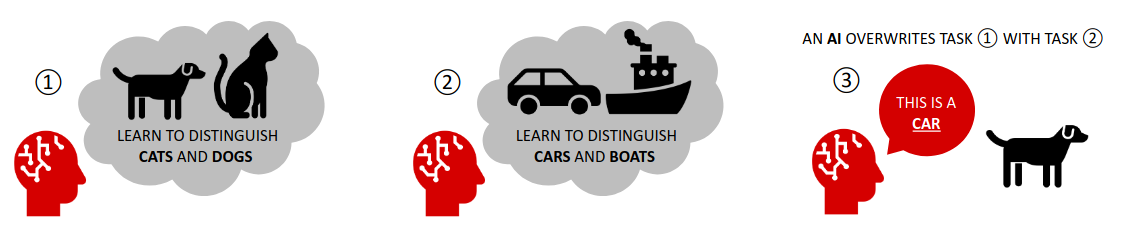
\includegraphics[width=0.75
    \textwidth]{images/CL2.png}
    \label{fig:MHA2}
\end{figure}

\subsection{Humans VS Neural Network}
\begin{wrapfigure}{r}{0.4\textwidth}
    \centering
    \vspace{-10pt}
    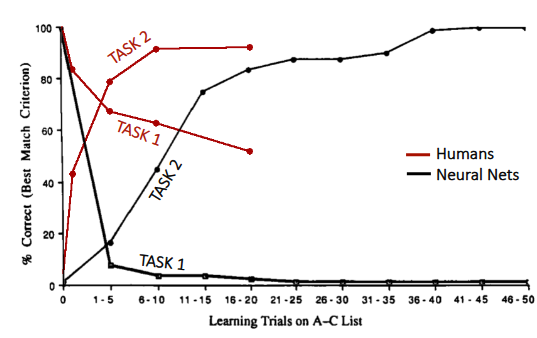
\includegraphics[width=\linewidth]{images/CL3.png}
    \label{fig:Scaled Dot Product Attention}
    \vspace{-10pt}
\end{wrapfigure}
The distinction between human forgetting and neural-network forgetting was highlighted
early in psychology. In 1959, \textbf{Barnes and Underwood} examined how humans learn two
sequential tasks. Participants learned word pairs such as home-star and field-sky (Task 1),
then learned modified pairs like home-field and field-car (Task 2). Results showed that hu-
mans do forget some of the initial associations: performance declines on Task 1 while im-
proving on Task 2. However, this degradation is \textbf{gradual}, not destructive.

In 1989, \textbf{McCloskey and Cohen} repeated the same two-task experiment using artificial
neural networks. Their findings were striking: networks did not simply become slightly worse on Task 1, they lost the ability to perform
it almost entirely after just a few learning steps on Task 2. The drop in performance was rapid, severe, and complete. This is why re-
searchers call it \textbf{catastrophic} forgetting: the forgetting is not merely present but overwhelmingly destructive, reducing earlier learning
to effectively zero.

\subsection{Why Do Neural Networks Forget?}
Catastrophic forgetting arises primarily from optimization using \textbf{gradient descent}. A neural
network is defined by its parameters $W$. Training on Task~A moves the parameters from a
random initialization $W_0$ to a solution $W_A$ that yields low error for that task. When the
network is later trained on Task~B, gradient descent modifies these same parameters, pushing
them toward another optimum $W_B$, often far from the region where Task~A performed well.
Task~A’s performance therefore collapses.  

Although neural networks are often \textbf{over-parameterized}, meaning that joint solutions $W_{A+B}$
capable of solving both tasks likely exist, standard optimization has no built-in mechanism to
preserve old knowledge. SGD simply follows the gradient of the new task, even when this drives
the model away from earlier solutions.

\begin{figure}[H]
    \centering
    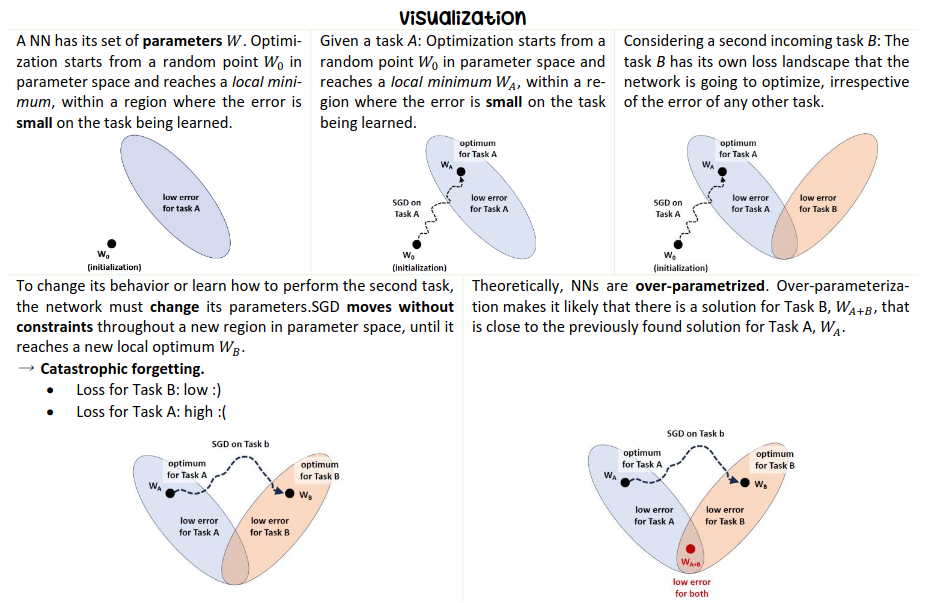
\includegraphics[width=1
    \textwidth]{images/CL4.png}
    \label{fig:MHA2}
\end{figure}

\textbf{Continual Learning (CL)} aims to overcome catastrophic forgetting by training models on streams of evolving data while preserving prior
knowledge. The goal is to constrain learning so that updates for Task B do not destroy the low-error region for Task A, even though the
model no longer has access to Task-A training examples. Achieving this without retraining from scratch is one of the central challenges
in continual learning.

CL has become a rapidly growing research area, with interest from both academia and indus-
try. Startups and large companies are exploring CL to build AI systems that adapt over time,
remain versatile, and avoid the catastrophic knowledge loss observed in standard neural net-
works. Trends in publications and search interest demonstrate increasing attention to this
field.

\subsection{A Common Continual Learning Scenario}
In a typical continual learning (CL) setting, a classification problem is divided into
$T$ sequential tasks. During each task $t \in \{1, \dots, T\}$, the model receives input
samples $x$ and labels $y$ drawn i.i.d.\ from a distribution $D_t$. A classic example is the
Split MNIST protocol, where the MNIST dataset is partitioned into 5 tasks, each containing two
digits (e.g., Task~1: 0/1, Task~2: 2/3, \dots, Task~5: 8/9). The model learns each task in
sequence, and past data are assumed to become unavailable as soon as training proceeds to the
next task.

\begin{figure}[H]
    \centering
    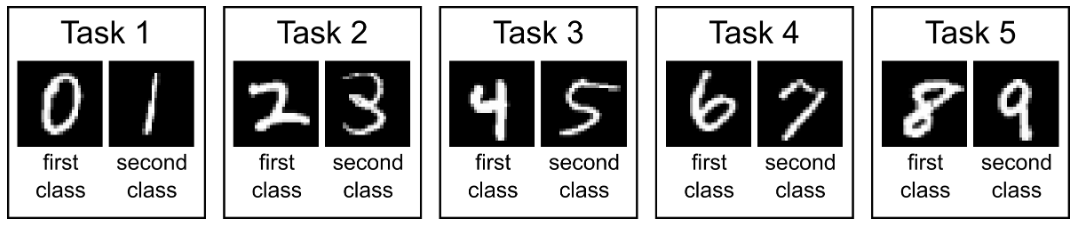
\includegraphics[width=0.8
    \textwidth]{images/CL5.png}
    \label{fig:MHA2}
\end{figure}
In scenarios such as \textbf{Task-IL} (Task-Incremental Learning), at the model is told which task an input
belongs to, for example, whether the image contains the first or the second class of the
current pair. A single function $f_\theta$ must be optimized sequentially, task after task,
over time.

This setting is important both in research and in industry. Real-world systems often face
streams of continuously arriving data, and retraining from scratch (joint training on all
past and present data) is extremely expensive or outright infeasible. Continual learning
methods aim to avoid this inefficiency.

\subsection{The Common Objective in CL}
The goal of continual learning is clear: at any point in training, the model should correctly
classify inputs from all tasks observed so far. Formally, at time $t_c$, we aim to minimize
the cumulative loss:
\[
\arg \min_{\theta} \sum_{t=1}^{t_c} \mathcal{L}_t
\quad \text{where} \quad
\mathcal{L}_t \equiv \mathbb{E}_{(x,y)\sim D_t}\bigl[\ell\bigl(y, f_\theta(x)\bigr)\bigr].
\]

The key challenge is that the data from previous tasks $D_1, \dots, D_{t_c-1}$ are assumed to
be \textbf{unavailable}. The model must find the best parameters for all tasks using only the current
dataset $D_{t_c}$. This makes the problem extremely challenging: we want the model to behave
well on tasks A and B while only seeing data from B.

Gradient descent makes this even more difficult because it is a \textbf{greedy} optimizer. At each
step, it changes parameters to reduce the loss on the current data subset. There is no
guarantee that these updates remain compatible with earlier tasks. In fact, as seen earlier,
vanilla fine-tuning almost always overwrites previously acquired knowledge.

\subsection{A NAÏVE Baseline: Joint Training}
One obvious solution would be to avoid forgetting entirely: simply retrain the model jointly on all available data from Tasks A and B.
This guarantees the best performance but is extremely inefficient and unrealistic, especially when data continue to arrive over time.
Continual learning explicitly avoids this “retrain-everything” approach by assuming that past data cannot be stored indefinitely.

\subsection{Elastic Weight Consolidation (EWC)}
One of the first influential methods developed to mitigate catastrophic forgetting is
\textbf{Elastic Weight Consolidation (EWC)}, introduced by Kirkpatrick et al.\ in 2017. EWC is
inspired by biological mechanisms, specifically the concept of \textbf{synaptic consolidation}
in the brain.

Humans do experience forgetting when learning tasks sequentially, but this forgetting is mild
and gradual, not destructive. This difference is partly due to biological mechanisms such as
\textbf{synaptic consolidation}: when humans learn something important, the corresponding neural
connections become more stable and resistant to change. As a result, when a new task is
learned, the brain does not overwrite earlier knowledge but adjusts only the connections that
are still flexible. In other words, humans have a natural form of \textbf{selective plasticity} that
preserves crucial information while continuing to learn.

Neural networks lack this mechanism by default. During gradient descent, all parameters remain
highly plastic and can be modified drastically. So when the model learns the second task, it
unintentionally overwrites parameter configurations that were essential for the first one.
This is why forgetting in humans is limited, while in machines it becomes catastrophic: in
just a few learning steps, the model can lose almost all ability to perform the earlier task.

So, in the brain:
\begin{compactitemize}
    \item biological \textbf{plasticity} allows the nervous system to adapt while preserving important
    synaptic strengths;
    \item \textbf{synapses} crucial to previously learned tasks become less plastic, protecting old
    memories from being overwritten.
\end{compactitemize}

EWC transfers this intuition to neural networks: parameters that were important for past tasks
should not change too much when learning a new one. It does so by adding a \textbf{quadratic penalty}
to the loss function that acts like an elastic "spring", pulling parameters back toward
their old values.

So, it can be imagined as a spring \textbf{anchoring} the parameters to the previous solution, hence
the name \textbf{elastic}. Importantly, the stiffness of this spring should not be the same for
all parameters; rather, \textbf{it should be greater} for those parameters that \textbf{matter most} to the
performance during Task~A.

\subsection{The EWC Loss Function}
When learning Task~B, the total loss optimized by EWC is:
\[
\mathcal{L}(\theta)
=
\mathcal{L}_B(\theta)
+
\sum_i \frac{\lambda}{2}
F_i \bigl(\theta_i - \theta^{*}_{A,i}\bigr)^2.
\]
\newpage
\begin{wrapfigure}{r}{0.4\textwidth}
    \centering
    \vspace{-10pt}
    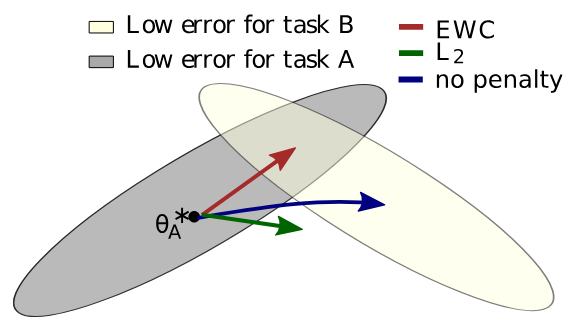
\includegraphics[width=\linewidth]{images/CL6.png}
    \label{fig:Scaled Dot Product Attention}
    \vspace{-10pt}
\end{wrapfigure}
Here:
\begin{compactitemize}
    \item $\mathcal{L}_B(\theta)$ is the standard loss for Task~B (typically cross-entropy, for
    classification);
    \item $\theta^{*}_A$ are the optimal parameters for Task~A;
    \item $F_i$ is the estimated importance of parameter $i$ for Task~A;
    \item $\lambda$ is a scaling hyperparameter balancing plasticity vs.\ stability.
\end{compactitemize}

Intuitively, this loss enforces two objectives:
\begin{enumerate}
    \item \textbf{learn Task~B well} by minimizing $\mathcal{L}_B$;
    \item \textbf{stay close to the Task~A solution} by minimizing the weighted squared distance between
    $\theta$ and $\theta^{*}_A$.
\end{enumerate}

If we momentarily ignore the importance weights and the scaling factors, the second term
essentially becomes $\bigl(\theta_i - \theta^{*}_{A,i}\bigr)^2$, which is simply the \text{squared
Euclidean distance} from the old optimum. In practice, this term encourages the updated
parameters to stay close to the values that previously worked well for Task~A, keeping the
new solution within its neighborhood.

\subsection{The Role of $F_i$}
The parameter-specific factor $F_i$:
\begin{compactitemize}
    \item is \textbf{not learnable};
    \item depends on the importance of each parameter for Task~A;
    \item controls how strongly that parameter should resist change.
\end{compactitemize}

If $F_i \approx 0$, the parameter is free to adapt to Task~B. If $F_i$ is large, the ``spring''
becomes stiff, preventing the parameter from moving far from its Task~A optimum.

\subsection{The Role of $\lambda$}
$\lambda$ adjusts the overall weight of the penalty. It controls the global trade-off between
retaining old knowledge (Task~A) and acquiring new knowledge (Task~B).

\subsection{Estimating Parameter Importance: The Fisher Information Matrix}
To compute the importance weights $F_i$, EWC uses the \textbf{diagonal of the empirical Fisher
Information Matrix (FIM)} computed at the Task~A optimal parameters:
\[
\mathcal{I}_{\theta_A^*}
=
\frac{1}{N}
\sum_{i=1}^{N}
\bigl[
\nabla_\theta \log p(x_A^{(i)} \mid \theta_A^*)
\bigr]
\bigl[
\nabla_\theta \log p(x_A^{(i)} \mid \theta_A^*)
\bigr]^{\top}.
\]

Because EWC uses only the diagonal, $F_i$ becomes:
\[
F_i
=
\frac{1}{N}
\sum_{k=1}^{N}
\left(
\frac{\partial \mathcal{L}(x_k)}{\partial \theta_i}
\right)^2.
\]

This quantity can be computed from squared gradients: simple, cheap, and efficient.

\subsection{Why Does Make Sense?}
The gradient magnitude $\left|\frac{\partial \mathcal{L}(x_i)}{\partial \theta_i}\right|$ measures how
sensitive the loss is to changes in parameter $\theta_i$:
\begin{compactitemize}
    \item if the gradient is \textbf{small}, perturbing $\theta_i$ barely affects performance
    $\rightarrow$ the parameter is not crucial $\rightarrow$ small penalty;
    \item if the gradient is \textbf{large}, even small changes harm performance
    $\rightarrow$ the parameter is important $\rightarrow$ large penalty.
\end{compactitemize}

Since EWC squares the gradient:
\begin{enumerate}
    \item the sign does not matter (only magnitude);
    \item bigger sensitivities are penalized more strongly.
\end{enumerate}

\subsection{Second-Derivative Interpretation}
\begin{wrapfigure}{r}{0.3\textwidth}
    \centering
    \vspace{-10pt}
    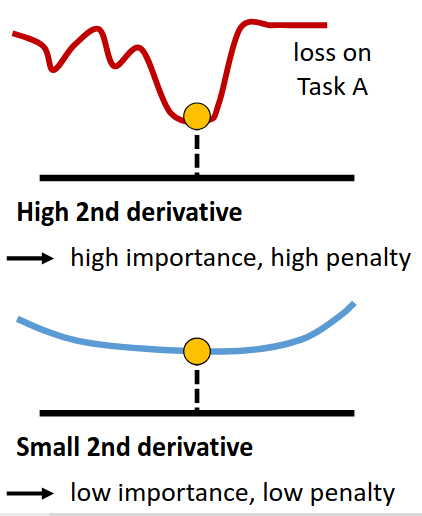
\includegraphics[width=\linewidth]{images/CL7.png}
    \label{fig:Scaled Dot Product Attention}
    \vspace{-10pt}
\end{wrapfigure}
There is also a geometric interpretation. Near a minimum, the second derivative of the loss
describes the curvature of the local region:
\begin{compactitemize}
    \item \textbf{high curvature} (sharp minimum) $\rightarrow$ loss increases rapidly
    $\rightarrow$ the corresponding weight must not move
    $\rightarrow$ high Fisher information $\rightarrow$ strong penalty.
    Few degrees of freedom;
    \item \textbf{low curvature} (flat minimum) $\rightarrow$ weight can change with little harm
    $\rightarrow$ low Fisher information $\rightarrow$ weak penalty.
    Many degrees of freedom.
\end{compactitemize}

Thus, the FIM acts as a proxy for the local geometry of the loss landscape around
$\theta_A^{*}$. This captures how many "degrees of freedom" the model has when adapting
to Task~B without corrupting Task~A.

\section{Continual Learning}

\subsection{Continual Learning Benchmarks}
Continual Learning (CL) methods are traditionally evaluated on simplified and highly controlled
image-classification benchmarks. These settings are designed to isolate specific challenges of
learning over time while avoiding confounding factors such as dataset noise or large-scale
training costs.

\begin{compactitemize}
    \item A common family of benchmarks is based on sequential tasks. For example, in \textbf{Sequential
    MNIST}, the classification problem is split into multiple subtasks: Task~1 consists of
    distinguishing digits 0 vs.\ 1, Task~2 focuses on digits 2 vs.\ 3, and so on. Similarly,
    \textbf{Sequential CIFAR} defines a sequence of binary classification problems, such as
    airplane vs.\ car in Task~1 and bird vs.\ cat in Task~2.
    
    \item Other benchmarks introduce structured changes to the input distribution. In \textbf{Rotated
    MNIST}, each task presents digit images rotated by a different angle, requiring the model
    to cope with domain shifts.
    
    \item In \textbf{Permuted MNIST}, every task applies a different fixed pixel permutation, generating
    distinct yet related classification problems.
\end{compactitemize}

Although more realistic benchmarks involving long and complex sequences of tasks exist, they
are often \textbf{computationally demanding}. For this reason, the community still relies heavily on
these abstract yet manageable setups.

\subsection{Evaluation Protocol}
Evaluation in Continual Learning typically relies on predefined train/test splits for each
task.

\begin{compactitemize}
    \item During \textbf{training}, tasks are presented sequentially: the model learns one task at a time,
    without revisiting data from previous tasks. Multiple training epochs per task are usually
    allowed to ensure that the model can fit each new task adequately.

    \item In the \textbf{testing} phase, the model is evaluated jointly on all test sets from every task
    encountered so far, regardless of order. This provides a measure of how well the model retains
    past knowledge while learning new information. Multiple epochs are usually allowed on each
    task, so that the model can fit the current task well.

\end{compactitemize}

A significant limitation of current CL research is the lack of unified hyperparameter tuning
protocols. Cross-validation and hyperparameter search strategies vary widely across studies,
making reproducibility and fair comparison challenging. Unfortunately, no established and
common practices already exist.

\subsection{Metrics}
The most commonly used metric in Continual Learning is \textbf{Average Accuracy (ACC)}. Let
$R_{i,j}$ denote the accuracy on task $t_j$ after the model has finished learning task $t_i$.
Once all $T$ tasks have been learned, ACC is defined as:
\[
\text{ACC}
=
\frac{1}{T}
\sum_{i=1}^{T}
R_{T,i}.
\]

This provides an overall assessment of the model’s performance on all tasks after the final
task has been trained. It can also be computed at intermediate points to track performance
progression.

Beyond ACC, other metrics are sometimes adopted, such as \textbf{Backward Transfer (BWT)},
which measures how much learning new tasks influences performance on old ones, and
\textbf{Forward Transfer (FWT)}, which measures whether learning earlier tasks helps
generalize to future ones. These were introduced by Lopez-Paz et al.\ in
\emph{Gradient Episodic Memory for Continual Learning}.

\subsection{Evaluation and Metrics}
\begin{figure}[H]
    \centering
    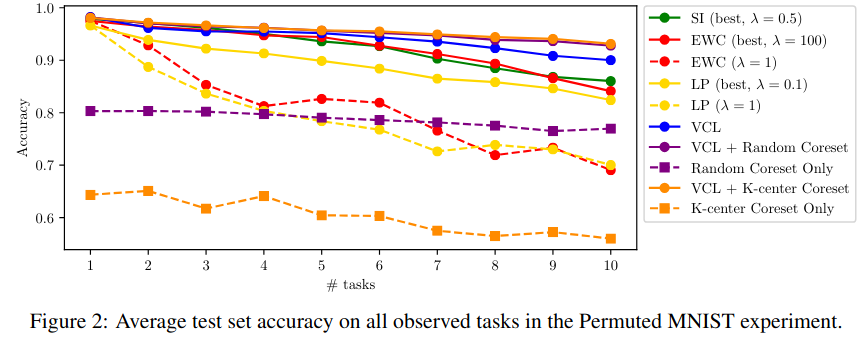
\includegraphics[width=0.9
    \textwidth]{images/CL8.png}
    \label{fig:MHA2}
\end{figure}

We can use plots like this to visualize the accuracy achieved on different tasks (shown on the x-axis) by various models. A common
pattern emerges: accuracy tends to decrease as the number of learned tasks grows. This is intuitive: each additional task increases the
range of concepts the model must recognize, and managing a larger set of tasks typically leads to progressively worse performance

\subsection{Evaluation Scenarios}
Continual Learning scenarios can differ significantly depending on what information is
available at test time and how tasks are defined. Three scenarios are most commonly
considered:

\begin{enumerate}
    \item \textbf{Task-Incremental Learning (Task-IL):}  
    In Task-IL, the model learns each task separately. During testing, the
    \textbf{identity of the task} associated with each input example \textbf{is provided}. This
    allows the system to select the appropriate output head or sub-module for that task.
    Task-IL is therefore the simplest scenario, as the model does not need to infer which
    task the test example belongs to.

    \begin{center}
        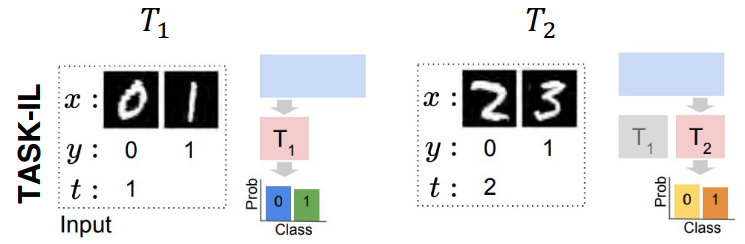
\includegraphics[width=0.6\textwidth]{images/CL9}
    \end{center}

    \item \textbf{Class-Incremental Learning (Class-IL):}  
    As in Task-IL, training occurs on one task at a time. However, at test time,
    \textbf{task identity is not given}. The model must predict the correct class among
    all classes observed so far. This setting is significantly more challenging, as it
    requires the model to integrate all knowledge accumulated across tasks into a unified
    classifier.

    \begin{center}
        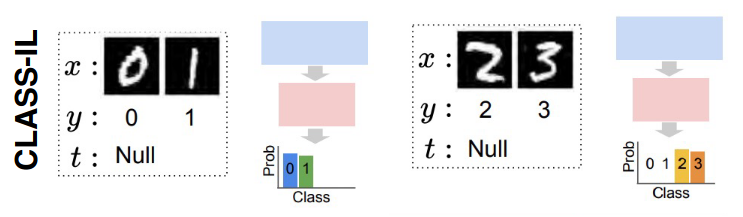
\includegraphics[width=0.6\textwidth]{images/CL10}
    \end{center}

    \item \textbf{Domain-Incremental Learning (Domain-IL):}  
    In Domain-IL, \textbf{the set of classes remains constant across tasks, but the input
    distribution changes}. Each task introduces a domain shift, such as image rotations or
    pixel permutations. The model must adapt to the new domain while preserving performance
    on the previous ones.

    \begin{center}
        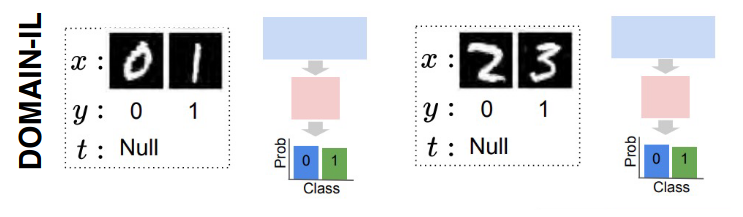
\includegraphics[width=0.6\textwidth]{images/CL11}
    \end{center}
\end{enumerate}

\subsection{Other Scenario in the Literature}

Additional scenarios broaden the conceptual space of Continual Learning.

$\rightarrow$ \textbf{General Continual Learning (GCL)} removes the notion of discrete tasks
entirely. Instead, the data distribution evolves smoothly over time, and the learner must
adapt continuously.
\begin{wrapfigure}{r}{0.3\textwidth}
    \centering
    \vspace{-10pt}
    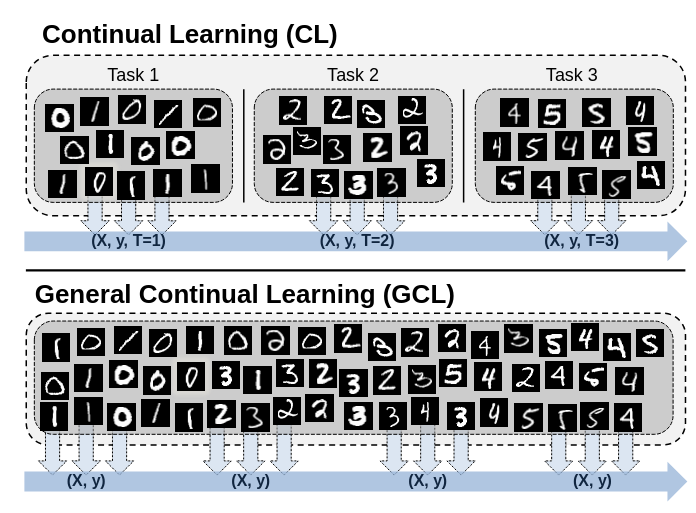
\includegraphics[width=\linewidth]{images/CL12.png}
    \label{fig:Scaled Dot Product Attention}
    \vspace{-10pt}
\end{wrapfigure}
$\rightarrow$ \textbf{Online Class-IL} and \textbf{Online Task-IL} impose stricter constraints
by allowing only a single pass (one epoch) over each task’s data, making the setting closer to
realistic streaming data scenarios.

$\rightarrow$ \textbf{Continual semi-supervised} or \textbf{self-supervised learning} extends
the problem to cases where labels are partially available or completely absent.

$\rightarrow$ \textbf{Data-Incremental Learning (Data-IL)} assumes that the set of classes is
fixed, and tasks correspond to different, possibly sequential partitions of the dataset.

In this course, the focus is on \textbf{Class-Incremental Learning}, as it is the most widely
studied and arguably the most difficult setting.

\subsection{A Taxonomy of Continual Learning Approaches}
\begin{wrapfigure}{r}{0.4\textwidth}
    \centering
    \vspace{-10pt}
    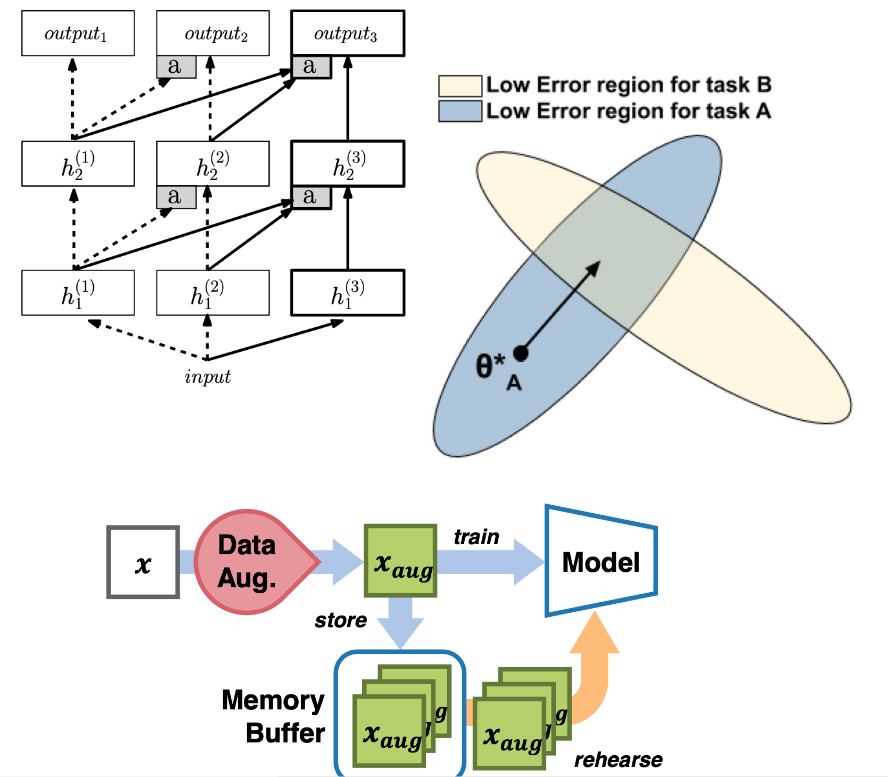
\includegraphics[width=\linewidth]{images/CL13.png}
    \label{fig:Scaled Dot Product Attention}
    \vspace{-10pt}
\end{wrapfigure}

CL methods are commonly grouped into three categories:

(A) \textbf{Architectural Methods}: These approaches allocate dedicated sub-networks or
components for different tasks. They often achieve excellent performance but typically
require increasing memory or model size as tasks accumulate.

(B) \textbf{Regularization Methods}: These introduce additional loss terms to prevent the
model from altering parameters critical for previously learned tasks. Examples include
weight-importance methods (e.g., Elastic Weight Consolidation) and knowledge
distillation--based approaches. They maintain bounded memory requirements and scale well
to long task sequences.

(C) \textbf{Replay Methods}: Replay approaches store selected examples from previous tasks in
a memory buffer. These samples are replayed during training on new tasks to prevent
forgetting. Replay is effective and conceptually straightforward, but performance generally
increases with the size of the memory buffer, making memory constraints a practical issue.

\section{(A) Architectural Methods}

\subsection{Weight Sharing}
A major source of \textbf{catastrophic forgetting} in neural networks is the \textbf{shared set of parameters} across multiple tasks. When a model learns
a new task, updates applied during training can overwrite the optimal parameter configuration that was previously learned for past
tasks. This \textbf{inter-task interference} arises because all incremental tasks are forced to share a single parameter space, making it difficult
to retain earlier knowledge.

The central question in Continual Learning is: how can we mitigate this interference and preserve past knowledge while still learning
new tasks effectively?

\subsection{Architectural Approaches}

One strategy to address inter-task interference is through \textbf{architectural methods}, which allocate distinct sub-models or task-specific
parameters for each task. The main idea is to \textbf{add new parameters for new tasks}, effectively isolating them from those used in previous
tasks. By doing so, the parameters for earlier tasks can be fixed, ensuring \textbf{maximal stability}.

\subsection{Progressive Neural Networks (PNN)}
\begin{wrapfigure}{r}{0.25\textwidth}
    \centering
    \vspace{-10pt}
    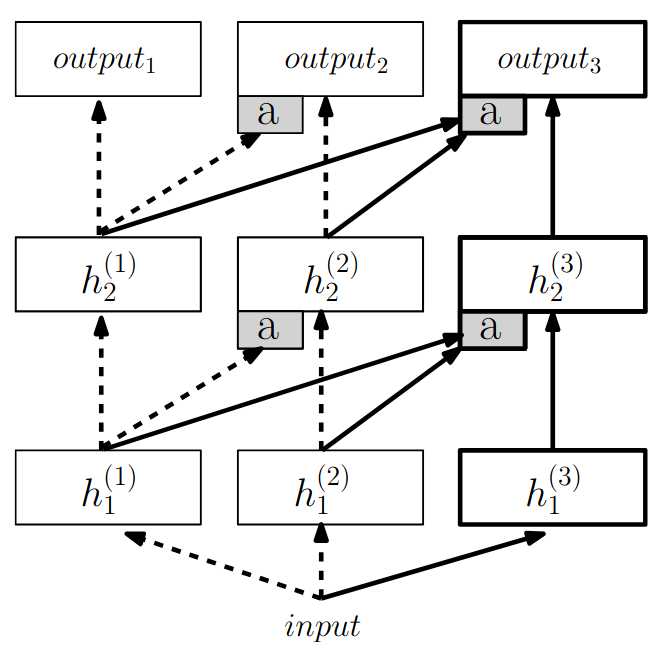
\includegraphics[width=\linewidth]{images/CL14.png}
    \label{fig:Scaled Dot Product Attention}
    \vspace{-10pt}
\end{wrapfigure}
An influential example of architectural approaches is \textbf{Progressive Neural Networks
(PNN)}, proposed by Rusu et al.\ (2016). In PNN:

$\rightarrow$ A new neural network column is instantiated for each incoming task.

$\rightarrow$ Catastrophic forgetting is \textbf{prevented} because each task has its own
dedicated parameters.

$\rightarrow$ Knowledge transfer is enabled via \textbf{lateral connections} from previously
learned columns, allowing the network to reuse prior computations.

\vspace{0.3cm}

\begin{center}
    \hrule
    \vspace{0.3cm}
    
    \begin{minipage}[t]{0.47\textwidth}
    \centering
    \textbf{Advantages of PNN}
    
    \vspace{0.2cm}
    \hrule
    \vspace{0.2cm}
    
    $\rightarrow$ \textbf{Immunity to catastrophic forgetting} by design.
    
    \vspace{0.15cm}
    
    $\rightarrow$ \textbf{Knowledge reuse}:through lateral connections, allowing new tasks to leverage
    previously learned features.
    
    \end{minipage}
    \hfill
    \begin{minipage}[t]{0.47\textwidth}
    \centering
    \textbf{Disadvantages of PNN}
    
    \vspace{0.2cm}
    \hrule
    \vspace{0.2cm}
    
    $\rightarrow$ \textbf{Scalability issues}: the number of parameters grows with each new task, leading
    to high memory requirements.
    
    \vspace{0.15cm}
    
    $\rightarrow$ \textbf{Task-IL only}: inference requires knowledge of the task label to select the
    appropriate column.
    
    \end{minipage}
    
    \vspace{0.3cm}
\hrule
\end{center}
\vspace{0.3cm}
To mitigate the scalability problem, later methods explored reducing the amount of new
capacity added for each task, for instance by pruning unused neurons or compressing
networks online. Examples of such methods include \textbf{PackNet}, \textbf{PathNet},
\textbf{Piggyback}, and \textbf{HAT} (Hard Attention to the Task).

\subsection{PackNet}

\textbf{PackNet} (Mallya et al.) exploits the redundancy present in large deep networks to
sequentially pack multiple tasks into a single network with minimal performance loss. The
method works as follows:

(1) Train the network for the first task and identify the most important weights.

(2) Prune a fraction of less important weights (e.g., 60\%) and retrain to recover performance
on the first task.

(3) Fixed weights are preserved, while the freed parameters are used to learn subsequent tasks.

This iterative pruning and retraining procedure allows multiple tasks to share the same
network without catastrophic forgetting, while significantly reducing memory overhead
compared to naive architectural expansion.


\begin{figure}[H]
    \centering
    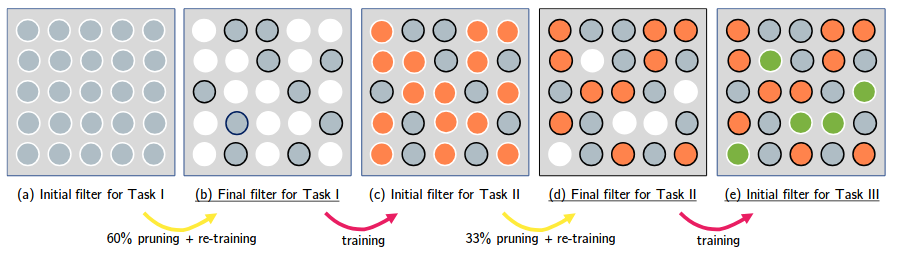
\includegraphics[width=0.9
    \textwidth]{images/CL15.png}
    \label{fig:MHA2}
\end{figure}

\subsection{Example: PackNet with Three Tasks}

Suppose we have a neural network with a large number of parameters, and we want to train it
sequentially on \textbf{three tasks}: Task~A, Task~B, and Task~C.

\vspace{0.3cm}
\hrule
\vspace{0.15cm}

\textbf{Step 1 --- Train on Task A and Prune the Network}

$\rightarrow$ We train the full network on Task~A until it achieves good performance.

$\rightarrow$ After training, we identify the most important weights for Task~A (e.g., using
magnitude-based criteria or other importance measures).

$\rightarrow$ We prune a fraction of the network’s weights that are \textbf{less important}
for Task~A (for example, pruning 60\% of the weights).

$\rightarrow$ The remaining weights, which are crucial for Task~A, are \textbf{frozen} and
cannot be updated anymore.

\vspace{0.3cm}
\hrule

\vspace{0.3cm}

\textbf{Step 2 --- Train on Task B}

$\rightarrow$ The network is retrained to recover any performance lost due to pruning.

$\rightarrow$ The \textbf{freed weights} resulting from the pruning process are used to train
the network on Task~B.

$\rightarrow$ Frozen weights from Task~A ensure that performance on Task~A is preserved.

$\rightarrow$ After training Task~B, the same procedure can be repeated: less important weights
are pruned and important ones are frozen.

\vspace{0.3cm}
\hrule
\vspace{0.3cm}

\textbf{Step 3 --- Train on Task C}

$\rightarrow$ The remaining available parameters are now used to learn Task~C.

$\rightarrow$ Weights frozen after Tasks~A and~B prevent forgetting of the previously learned
tasks.

\vspace{0.3cm}
\hrule
\vspace{0.3cm}

\textbf{Result}

$\rightarrow$ Each task is learned sequentially within the \textbf{same network}, without
catastrophic forgetting.

$\rightarrow$ Parameters are efficiently reused: only unimportant weights are reallocated for
new tasks.

$\rightarrow$ Memory overhead is minimal compared to methods that allocate a new network for
each task (e.g., Progressive Neural Networks).

\vspace{0.3cm}
\hrule
\vspace{0.3cm}

\textbf{Intuition}: Think of the network as a \emph{packing container}: Task~A fills some space, then pruning frees
unused slots. Task~B occupies the freed slots, and so on. Each task gets its own dedicated
``section'' in the same network, while the old sections remain intact.

\textbf{Inference Step in PackNet}:

(1) \textbf{Identify the task of the example}: In PackNet, \textbf{task identity is required at
test time}. The model must know which task the input belongs to (Task~A, Task~B, or Task~C).

(2) \textbf{Select the correct subset of weights}: Only the parameters assigned to the
corresponding task are activated. Weights frozen for other tasks remain unchanged.

(3) \textbf{Forward pass}: The input is processed through the network using only the relevant
parameters for the selected task.

(4) \textbf{Output}: The network produces the prediction for that task. Since weights from
previous tasks are frozen, the model does not forget how to solve earlier tasks.

\chapter{Federated Learning}

\section{Introduction to Federated Learning}

\subsection{Recap: Centralized Machine Learning}
Until now we have seen only a centralized machine learning that has some characteristics, that include:
\begin{compactitemize}
    \item \textbf{All data in one place}: Training data from alla sources is aggregated and stored on a central server or in a data center. The model has access to the entire dataset during training.
    \item \textbf{Single model, combined dataset}: A single global model is trained oh this unified dataset. This traditional approach relied on processing all data centrally before model training.
    \item \textbf{Iterative optimization (SGD)}:The model's parameters are iteratively updated using SGD, epoch after epoch until the model converges.
\end{compactitemize}

\subsection{Problems Motivating Decentralized and Federated Learning}

In many real-world scenarios, the traditional paradigm of \textbf{centralized machine
learning}—where all data are collected and stored on a single server—is either impractical
or undesirable. Several fundamental challenges motivate the need for decentralized and
federated learning approaches.

\begin{compactitemize}
    \item \textbf{Data privacy and confidentiality.}  
    Many application domains involve \textbf{sensitive data}, such as personal information,
    medical records, or financial transactions. Transferring these data to a central server
    raises serious privacy risks and increases exposure to data breaches. In such settings,
    data should ideally \textbf{remain on-device or on-premise}, and only model-related
    information should be shared.

    \item \textbf{Bandwidth limitations and data scale.}  
    Modern datasets are often extremely large, making data centralization costly or
    infeasible. Uploading raw data from millions of edge devices would require enormous
    communication bandwidth and incur high latency. In contrast, sharing compact model
    updates is significantly more efficient.

    \item \textbf{Exploiting distributed computational resources.}  
    Edge devices such as smartphones, IoT devices, and local servers possess substantial
    computational power. Decentralized learning frameworks allow these clients to perform
    most of the computation locally, reducing the load on central servers and enabling
    better scalability.

    \item \textbf{Regulatory and legal constraints.}  
    Data protection regulations such as \textbf{GDPR}, \textbf{HIPAA}, and similar legal
    frameworks impose strict constraints on how data can be stored, processed, and shared.
    Keeping data localized while exchanging only model updates helps ensure compliance with
    these regulations.
\end{compactitemize}

Together, these challenges highlight the limitations of centralized learning and motivate
learning paradigms in which \textbf{data remain decentralized}, while models are trained
collaboratively across multiple clients. This setting naturally leads to approaches such as
\textbf{Federated Learning}, which aim to balance privacy, efficiency, and scalability.

\subsection{Solution: Federated Learning}

\textbf{Federated Learning (FL)} is a distributed machine learning paradigm designed to
address the limitations of centralized training in privacy-sensitive and large-scale
settings. In Federated Learning, a \textbf{central server} coordinates a population of
\textbf{clients} (e.g., mobile devices, hospitals, companies) to collaboratively train a
shared model \textbf{without collecting or centralizing raw data}.

Each client keeps its local dataset private and performs training locally. Only
\textbf{model updates}—such as weights or gradients—are communicated to the server, which
aggregates them to form a global model. This approach enables learning from decentralized
data while improving privacy, reducing communication costs, and exploiting distributed
compute resources.

\textbf{Key idea:} \emph{keep data local, share only model updates.}
\begin{figure}[H]
    \centering
    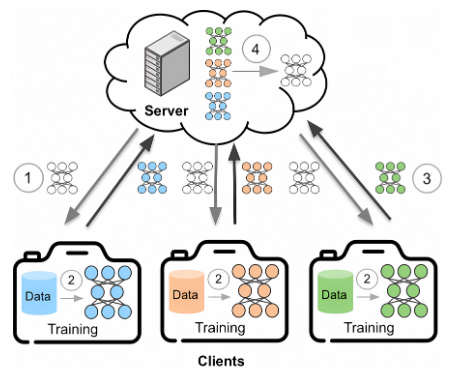
\includegraphics[width=0.5
    \textwidth]{images/FL1.png}
    \label{fig:MHA2}
\end{figure}

\vspace{0.3cm}

\begin{center}
    \hrule
    \vspace{0.3cm}
    
    \begin{minipage}[t]{0.47\textwidth}
    \centering
    \textbf{Client-side Objective}
    
    \vspace{0.2cm}
    \hrule
    \vspace{0.2cm}
    
    Each client $i$ holds a private dataset $D_i$.  
    The client optimizes its local model parameters $\theta_i$ by minimizing the loss
    using only its own data:
    
    \[
    \min_{\theta_i}
    \;
    \mathbb{E}_{(x,y)\sim D_i}
    \bigl[
    \mathcal{L}\bigl(f_{\theta_i}(x), y\bigr)
    \bigr].
    \]
    
    \vspace{0.15cm}
    
    Local training is performed independently and no raw data are shared with the server
    or other clients.
    
    \end{minipage}
    \hfill
    \begin{minipage}[t]{0.47\textwidth}
    \centering
    \textbf{Server-side Objective}
    
    \vspace{0.2cm}
    \hrule
    \vspace{0.2cm}
    
    The server has \textbf{no access to data}. Its goal is to obtain a global model
    $\theta$ that minimizes the average loss across all $N$ clients:
    
    \[
    \min_{\theta}
    \;
    \frac{1}{N}
    \sum_{i=1}^{N}
    \mathbb{E}_{(x,y)\sim D_i}
    \bigl[
    \mathcal{L}\bigl(f_{\theta}(x), y\bigr)
    \bigr].
    \]
    
    \vspace{0.15cm}
    
    This objective is achieved by aggregating local updates received from the clients.
    
    \end{minipage}
    
    \vspace{0.3cm}
\hrule
\end{center}

\vspace{0.3cm}

This formulation highlights the fundamental asymmetry of Federated Learning: \textbf{clients
optimize locally using private data}, while the \textbf{server coordinates and aggregates}
without ever observing raw samples. As a result, FL provides a principled solution to
privacy, scalability, and regulatory challenges in modern distributed learning systems.

\subsection{Application Scenarios}

Federated Learning can be applied in different real-world settings depending on the number
of participating clients and the characteristics of their local datasets. Two main
application scenarios are commonly distinguished.

\begin{compactitemize}
    \item \textbf{Cross-device Federated Learning.}  
    This scenario involves a \textbf{massive number of edge devices}, such as smartphones,
    wearables, or IoT sensors. Each device typically holds only a \textbf{small amount of
    data}, and participation is often intermittent due to connectivity or energy
    constraints.  
    A canonical example is training a \textbf{mobile keyboard or language model} directly
    on users’ phones, where sensitive information such as keystrokes remains on-device and
    is never uploaded to a central server.

    \item \textbf{Cross-silo Federated Learning.}  
    In this setting, the number of clients is relatively \textbf{small}, but each client
    (or silo) owns a \textbf{large and rich local dataset}. Typical clients include
    organizations such as hospitals, banks, or research institutions.  
    A representative example is multiple \textbf{hospitals collaboratively training a
    medical diagnostic model} without sharing patient records, thereby preserving privacy
    and complying with data protection regulations.
\end{compactitemize}

These two scenarios differ significantly in scale, communication patterns, and system
constraints, but both share the core principle of Federated Learning: \textbf{collaborative
training without data centralization}.

\subsection{Weight Averaging and Model Merging}

A fundamental mechanism underlying Federated Learning is \textbf{weight averaging}, also
referred to as \textbf{model merging}. This procedure enables a central server to improve a
global model by aggregating locally trained models, even though it has \textbf{no access to
any training data}.

The federated training process proceeds iteratively as follows:

\begin{enumerate}
    \item \textbf{Initialization.}  
    The server initializes a global model $\theta^{(0)}$. The server holds \textbf{no data},
    as all training samples are distributed across the clients.

    \item \textbf{Broadcast.}  
    At each communication round, the server selects a subset of clients and \textbf{sends
    the current global model} to them.

    \item \textbf{Local training.}  
    Each selected client performs local optimization on its private dataset for one or more
    epochs, obtaining an updated set of parameters based solely on local data.

    \item \textbf{Upload of updates.}  
    After local training, clients \textbf{send their model updates}—such as gradients or
    updated weights—back to the server.

    \item \textbf{Aggregation.}  
    The server \textbf{aggregates the received updates}, typically by computing a weighted
    or unweighted average, to obtain an improved global model.

\end{enumerate}

These steps are repeated until convergence. Through repeated rounds of local training and
global aggregation, the server progressively refines the global model without ever
observing raw client data.


\subsection{Key Challenges in Federated Learning}

Despite its advantages, Federated Learning introduces a number of fundamental challenges
that distinguish it from standard centralized training.

\begin{compactitemize}
    \item \textbf{Data heterogeneity (non-IID data).}  
    Clients typically possess data drawn from \textbf{different and potentially skewed
    distributions}. This non-IID setting can lead to \textbf{client drift}, where local
    updates move model parameters in conflicting directions, often resulting in slower
    convergence and reduced global accuracy.

    \item \textbf{Partial participation.}  
    In each communication round, only a \textbf{subset of clients} is available or willing
    to participate. The active client set may change across rounds due to stragglers,
    drop-outs, or connectivity constraints, introducing instability in the training
    process.

    \item \textbf{Communication overhead.}  
    Communication is often the main bottleneck in FL. Limited network capacity and high
    latency make it crucial to \textbf{minimize the size and frequency of model updates}
    exchanged between clients and the server in order to achieve efficient training.

    \item \textbf{Privacy and security.}  
    Although raw data remain local, \textbf{model updates can still leak sensitive
    information}. Adversarial attacks such as gradient inversion or membership inference
    highlight the need for additional privacy-preserving and security mechanisms.
\end{compactitemize}

Addressing these challenges is essential for making Federated Learning robust, scalable,
and deployable in real-world environments.

\section{Federated Averaging (FedAvg)}

\textbf{Federated Averaging (FedAvg)} is the foundational algorithm for Federated Learning,
introduced by McMahan et al.\ It provides a simple yet effective strategy for training a
global model from decentralized client updates.

At each communication round, the server selects a subset of clients and sends them the
current global model. Each selected client trains the model locally using its private data
for a fixed number of epochs and then returns the updated model parameters to the server.
The server combines these updates to obtain a new global model. This iterative procedure
is repeated over multiple rounds until convergence.

The key question addressed by FedAvg is:

\begin{center}
\emph{How should client updates be combined to form an improved global model?}
\end{center}

FedAvg answers this question using a \textbf{weighted averaging scheme}, where each
client’s contribution is proportional to the size of its local dataset. In this way,
clients with more data have a stronger influence on the global model, better approximating
the objective of minimizing the average loss across all clients.

\subsection{FedAvg Algorithm}

\vspace{0.3cm}

\noindent\rule{\textwidth}{0.8pt}

\noindent\textbf{Initialize:}  
Server initializes global model parameters $w_0$.

\noindent\textbf{for} communication rounds $t = 1, 2, \dots, T$ \textbf{do}

\noindent\hspace{0.6cm}\textbf{Client selection:}  
\noindent\hspace{0.6cm}Server selects a subset $C_t$ of available clients.

\noindent\hspace{0.6cm}\textbf{Broadcast:}  
\noindent\hspace{0.6cm}Server sends the current global model $w_{t-1}$ to all clients in $C_t$.

\noindent\hspace{0.6cm}\textbf{Local training:}  
\noindent\hspace{0.6cm}Each client $i \in C_t$ initializes its local model with $w_{t-1}$ and
performs local optimization (e.g., $E$ epochs of SGD) on its private dataset to obtain
updated parameters $w_t^{\,i}$.

\noindent\hspace{0.6cm}\textbf{Upload:}  
\noindent\hspace{0.6cm}Each client sends its updated model parameters $w_t^{\,i}$ (or the
model difference) back to the server.

\noindent\hspace{0.6cm}\textbf{Aggregation:}  
\noindent\hspace{0.6cm}Server aggregates the client models to form the new global model:
\[
w_t
\leftarrow
\sum_{i \in C_t}
\frac{n_i}{\sum_{j \in C_t} n_j}
\,
w_t^{\,i},
\]
where $n_i$ denotes the number of training samples at client $i$.

\noindent\textbf{end for}

\noindent\rule{\textwidth}{0.8pt}

\vspace{0.3cm}

Through repeated rounds of local training and weighted aggregation, FedAvg approximates
centralized empirical risk minimization while preserving data locality and privacy.

\subsection{FedAvg: Take-Home Message}

Federated Averaging works well when client data are approximately \textbf{i.i.d.} and has
become the \textbf{de facto baseline} for federated learning experiments.

\textbf{Strengths}:
\begin{compactitemize}
    \item \textbf{Simplicity}: FedAvg is easy to implement and requires minimal coordination
    between clients and server.
    \item \textbf{Communication efficiency}: multiple local SGD steps are performed before
    synchronization, significantly reducing communication frequency compared to fully
    synchronized distributed SGD.
\end{compactitemize}

\textbf{Limitations}:
\begin{compactitemize}
    \item \textbf{Sensitivity to non-IID data}: when client data distributions differ
    substantially, local models may drift toward different regions of the parameter space.
    \item \textbf{Client drift}: if local gradients point toward \emph{different directions},
    their average may no longer represent a meaningful descent direction for the global
    objective, harming convergence and final accuracy.
\end{compactitemize}

Intuitively, when gradients trend toward incompatible directions in the parameter space,
\textbf{simple averaging becomes ineffective}. As a consequence, the aggregated model may
fail to improve—or may even degrade—global performance.

These limitations have motivated a large body of work proposing \textbf{enhancements to
FedAvg}. Common strategies include modifying the local objective with additional
regularization terms (e.g., proximal constraints) or improving the aggregation procedure.
Next, we discuss the main families of approaches developed to address these challenges.

\subsection{Possible Improvements over FedAvg}

The limitations of FedAvg in heterogeneous settings have led to a variety of improved
federated learning methods. These approaches can be broadly categorized into three main
families.

\begin{compactitemize}
    \item \textbf{Server-side approaches.}  
    The server employs more sophisticated aggregation strategies instead of simple averaging.
    These methods aim to better align client updates or correct for bias introduced by
    heterogeneous data distributions.

    \item \textbf{Client-side approaches.}  
    Each client augments its local objective with additional terms—such as regularization or
    proximal constraints—that enforce \textbf{consistency with the global model}. This helps
    limit client drift during local training.

    \item \textbf{Prototype-based approaches.}  
    Constraints are enforced in \textbf{feature space} rather than directly in parameter
    space. By aligning class or representation prototypes across clients, these methods
    achieve a better trade-off between global consistency and local specialization.
\end{compactitemize}

These families of methods represent different ways of stabilizing federated optimization
under data heterogeneity, and form the foundation of many state-of-the-art federated
learning algorithms.

\section{Server-side Approach}

\subsection{Motivation for Fisher-Weighted Averaging}

Standard parameter averaging methods, such as \textbf{FedAvg}, treat every model parameter
as \textbf{equally informative}. Each weight dimension contributes uniformly to the
aggregation process, regardless of how important or reliable that parameter is for a
given client.

This assumption is reasonable when client updates are derived from \textbf{i.i.d. data}.
However, in federated settings with \textbf{data heterogeneity}, different clients may be
confident about different subsets of parameters. Uniform averaging can therefore be
sub-optimal, as it may dilute reliable parameters with noisy or conflicting updates.

\textbf{Key idea.}  
Instead of treating all parameters equally, the contribution of each model parameter should
be weighted by the \textbf{confidence} of the client in that parameter. This confidence can
be quantified using the \textbf{Fisher Information Matrix (FIM)}, which measures how
sensitive the model’s loss is to changes in each parameter.

By assigning higher weight to parameters with high Fisher information and lower weight to
less reliable ones, Fisher-weighted averaging aims to produce a global model that better
respects client-specific knowledge while remaining robust under heterogeneous data
distributions.


\subsection{Recall: Fisher Information Matrix}
\begin{wrapfigure}{r}{0.3\textwidth}
    \centering
    \vspace{-10pt}
    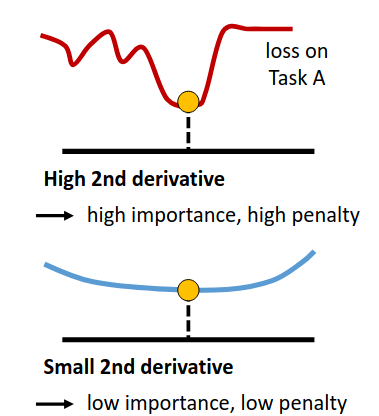
\includegraphics[width=\linewidth]{images/FL2.png}
    \label{fig:Scaled Dot Product Attention}
    \vspace{-10pt}
\end{wrapfigure}
One method previously discussed for estimating the importance of neural network parameters
is based on the \textbf{Fisher Information Matrix (FIM)}. The empirical Fisher Information
Matrix is defined as:
\[
F_\theta
=
\frac{1}{N}
\sum_{i=1}^{N}
\Bigl[
\nabla_\theta \log p\bigl(x^{(i)} \mid \theta\bigr)
\Bigr]
\Bigl[
\nabla_\theta \log p\bigl(x^{(i)} \mid \theta\bigr)
\Bigr]^{\top},
\]
where the gradients correspond to the derivatives of the loss function with respect to the
model parameters.

There exists a theoretical relationship between the empirical FIM and the \textbf{second
derivative of the loss function}. In particular, near a minimum, the Fisher Information
Matrix can be used as an approximation of the \textbf{Hessian matrix}.

Since the FIM captures the \textbf{local curvature} of the loss landscape:
\begin{compactitemize}
    \item a \textbf{high Fisher information} for a parameter indicates that the parameter is
    pivotal, and modifying it is likely to increase the loss;
    \item a \textbf{low Fisher information} indicates a flat region, meaning that small
    changes to the parameter have little effect on the loss.
\end{compactitemize}

\subsection{Fisher-Weighted Averaging: Core Formula}

Given $M$ client models $\{\theta_i\}_{i=1}^{M}$ with identical initialization, each client’s
posterior distribution is approximated as a Gaussian:
\[
p(\theta \mid \theta_i, F_i),
\]
where $F_i$ denotes the Fisher Information Matrix associated with client $i$.

The objective is to find the global model parameters $\theta^*$ that maximize the joint
posterior of all client models:
\[
\theta^*
=
\arg\max_{\theta}
\prod_{i=1}^{M}
\lambda_i \,
p(\theta \mid \theta_i, F_i),
\]
where $\lambda_i$ are scalar weights such that $\sum_i \lambda_i = 1$.

To simplify the optimization, all terms can be moved inside the logarithm:
\[
\theta^*
=
\arg\max_{\theta}
\sum_{i=1}^{M}
\lambda_i
\log p(\theta \mid \theta_i, F_i).
\]

This optimization problem admits a \textbf{closed-form solution}, given by:
\[
\theta^*
=
\left(
\sum_{i}
\lambda_i F_i
\right)^{-1}
\left(
\sum_{i}
\lambda_i F_i \theta_i
\right).
\]

\textbf{Practical considerations.}  
Estimating and storing the full Fisher Information Matrix is often infeasible for modern
neural networks due to their large number of parameters and over-parameterization.

A common solution is to use an \textbf{approximation of the FIM}, such as its diagonal. This
approximation can be represented as a vector and leads to a simplified aggregation rule:
\[
\theta^*
=
\frac{
\sum_{i=1}^{M}
\lambda_i F_i \theta_i
}{
\sum_{i=1}^{M}
\lambda_i F_i
}.
\]

This diagonal approximation makes Fisher-weighted averaging tractable in large-scale
federated learning settings.

\subsection{Practical Considerations in Federated Learning}

Fisher-weighted averaging introduces additional practical aspects that must be considered
when deploying the method in real federated learning systems.

\textbf{Computation of the Fisher Information.}  
The Fisher Information Matrix is typically computed \textbf{after each client finishes
local training}. In practice, only the \textbf{diagonal Fisher} is estimated, using the
squared gradients of the log-likelihood evaluated on a local mini-batch. This provides an
efficient approximation of parameter importance.

\textbf{Communication overhead.}  
Each client sends both the updated model parameters $\theta^{(k)}$ and the diagonal Fisher
$\mathrm{diag}(F^{(k)})$ to the server. Since both quantities are model-sized vectors, the
total communication payload is roughly doubled. However, this overhead is still practical
for typical federated learning models.

\textbf{Privacy considerations.}  
The Fisher Information Matrix does not reveal raw data, but only the \textbf{sensitivity of
the loss with respect to model parameters}. Nevertheless, it may still leak information.
For this reason, Fisher-weighted aggregation is often combined with \textbf{secure
aggregation} or \textbf{differential privacy} mechanisms.

\vspace{0.3cm}

The \textbf{strengths} of this approach are:
\begin{compactitemize}
    \item Improves accuracy over FedAvg on \textbf{heterogeneous data} by exploiting
    parameter importance.
    \item Tends to work particularly well when applied to \textbf{pretrained models} that
    share a common feature representation.
    \item Naturally supports \textbf{one-shot federated learning} or sporadic client
    participation, since models can be merged without requiring multiple communication
    rounds.
    \item Compatible with other \textbf{server-side techniques}, such as momentum or model
    quantization.
\end{compactitemize}

The \textbf{weaknesses} of this approach are:
\begin{compactitemize}
    \item Increased \textbf{client-side computation}, as multiple forward and backward
    passes are required to estimate the Fisher Information.
    \item Potential \textbf{numerical issues}, since the Fisher values may become very large
    or very small.
    \item Limited benefit when client models are \textbf{too far apart in parameter space},
    as the Fisher computed on local data may be meaningless when applied far from the local
    optimum.
\end{compactitemize}

\subsection{Derivation of Fisher-Weighted Averaging}
\begin{wrapfigure}{r}{0.4\textwidth}
    \centering
    \vspace{-10pt}
    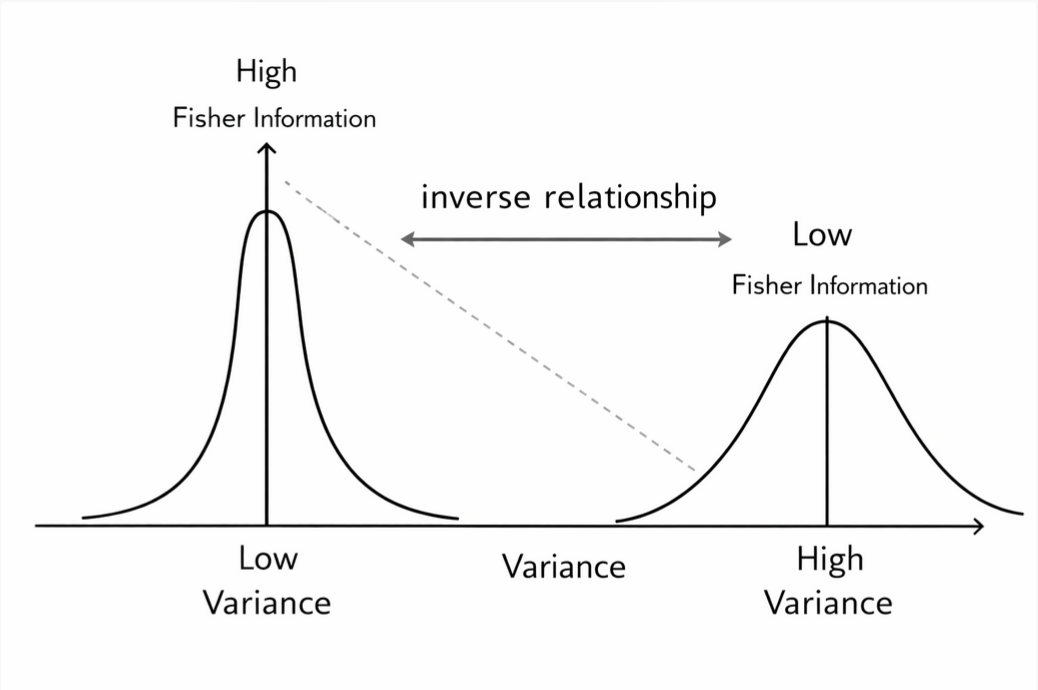
\includegraphics[width=\linewidth]{images/FL3.png}
    \label{fig:Scaled Dot Product Attention}
    \vspace{-10pt}
\end{wrapfigure}
\textbf{Setup.}  
After local training, each client $i = 1, \dots, M$ provides a parameter vector
$\theta_i \in \mathbb{R}^{n_p}$, where $n_p$ is the number of parameters of the network.
Each client also provides an estimate of parameter importance through the Fisher
Information Matrix $F_i \in \mathbb{R}^{n_p \times n_p}$, which is symmetric and positive
semi-definite.

We start by approximating the posterior distribution of each client as a Gaussian:
\[
p(\theta \mid \theta_i)
\;\approx\;
\mathcal{N}(\theta_i,\ \Sigma_i),
\]
where $\Sigma_i$ is the covariance matrix of the posterior around $\theta_i$.

Near a minimum, the inverse covariance can be approximated by the Fisher Information
Matrix:
\[
\Sigma_i^{-1} \;\approx\; F_i.
\]
As a result, the posterior can be rewritten as:
\[
p(\theta \mid \theta_i, F_i)
\;\approx\;
\mathcal{N}\bigl(\theta_i,\ F_i^{-1}\bigr),
\]
where $F_i$ acts as a \textbf{precision matrix}.  
Intuitively, a \textbf{low-variance posterior} corresponds to a \textbf{high Fisher
information} (high confidence), while a \textbf{high-variance posterior} corresponds to a
\textbf{low Fisher information} (low confidence).

The goal is to find the parameter vector $\theta^*$ that maximizes the joint posterior of
the $M$ independent client models:
\[
\theta^*
=
\arg\max_{\theta}
\prod_{i=1}^{M}
\lambda_i \, p(\theta \mid \theta_i, F_i),
\]
where $\lambda_i$ are scalar weights such that $\sum_i \lambda_i = 1$.

Taking the logarithm, this is equivalent to:
\[
\theta^*
=
\arg\max_{\theta}
\sum_{i=1}^{M}
\lambda_i \log p(\theta \mid \theta_i, F_i).
\]

\textbf{Gaussian form.}  
Since each posterior is Gaussian, the objective becomes:
\[
\theta^*
=
\arg\max_{\theta}
\sum_{i=1}^{M}
\lambda_i
\log
\left(
\exp\left\{
-\frac{1}{2}
(\theta - \theta_i)^\top
F_i
(\theta - \theta_i)
\right\}
\right).
\]

\textbf{Step 1 — Remove log and exponential.}  
Since $\log(\cdot)$ is monotone:
\[
\theta^*
=
\arg\max_{\theta}
-
\frac{1}{2}
\sum_{i=1}^{M}
\lambda_i
(\theta - \theta_i)^\top
F_i
(\theta - \theta_i).
\]

\textbf{Step 2 — Convert to minimization.}  
Multiplying by $-2$ yields the equivalent problem:
\[
\theta^*
=
\arg\min_{\theta}
\sum_{i=1}^{M}
\lambda_i
(\theta - \theta_i)^\top
F_i
(\theta - \theta_i).
\]

\textbf{Step 3 — Expand the quadratic forms.}
\[
\theta^*
=
\arg\min_{\theta}
\sum_{i=1}^{M}
\lambda_i
\Bigl(
\theta^\top F_i \theta
-
2 \theta^\top F_i \theta_i
+
\theta_i^\top F_i \theta_i
\Bigr).
\]
The last term does not depend on $\theta$ and can be removed from the optimization
problem.

\textbf{Step 4 — Collect terms.}
\[
\theta^*
=
\arg\min_{\theta}
\;
\theta^\top
\left(
\sum_{i=1}^{M} \lambda_i F_i
\right)
\theta
-
2
\theta^\top
\left(
\sum_{i=1}^{M} \lambda_i F_i \theta_i
\right).
\]

\textbf{Step 5 — Take the gradient and set it to zero.}  
Using symmetry of $F_i$:
\[
2
\left(
\sum_{i=1}^{M} \lambda_i F_i
\right)
\theta
-
2
\left(
\sum_{i=1}^{M} \lambda_i F_i \theta_i
\right)
= 0.
\]

\textbf{Step 6 — Solve for $\theta^*$.}
\[
\theta^*
=
\left(
\sum_{i=1}^{M} \lambda_i F_i
\right)^{-1}
\left(
\sum_{i=1}^{M} \lambda_i F_i \theta_i
\right).
\]

\textbf{Diagonal Fisher approximation.}  
If each $F_i$ is approximated by the diagonal of the Fisher Information Matrix, it can be
treated as a vector and the solution becomes element-wise:
\[
\theta^{*(j)}
=
\frac{
\sum_{i=1}^{M}
\lambda_i F_i^{(j)} \theta_i^{(j)}
}{
\sum_{i=1}^{M}
\lambda_i F_i^{(j)}
}.
\]

When all $F_i$ are identity matrices (i.e., all parameters are equally confident) and
$\lambda_i$ are proportional to the number of samples at each client, the solution reduces
to \textbf{standard weight averaging}, namely \textbf{FedAvg}.

\section{Client-Side Approach}
\subsection{The Client Drift Problem}
ith \textbf{non-i.i.d. data}, the local updates produced by different
clients may point toward \textbf{inconsistent directions}. This phenomenon is known as
\textbf{client drift} and represents one of the main limitations of FedAvg.

The core reason is that each client optimizes its model with respect to its \textbf{local
data distribution}. As a result, each client is driven toward its own local optimum, which
may differ significantly from the optimum of the global objective defined over all data.
Simply averaging these locally optimized models does not, in general, correspond to a
model obtained via joint training on the union of all datasets.
\begin{wrapfigure}{r}{0.4\textwidth}
    \centering
    \vspace{-10pt}
    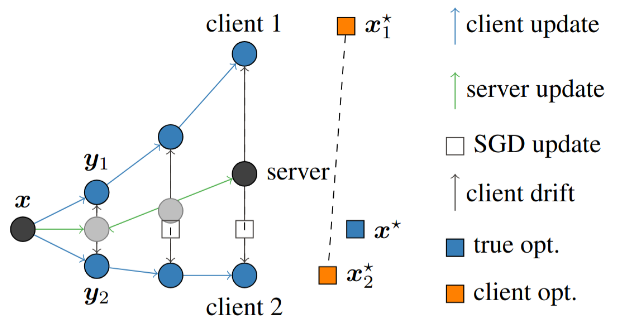
\includegraphics[width=\linewidth]{images/FL4.png}
    \label{fig:Scaled Dot Product Attention}
    \vspace{-10pt}
\end{wrapfigure}
In federated learning w
Client drift becomes increasingly severe as the data distributions across clients become
more \textbf{heterogeneous}. The problem is further exacerbated when only a \textbf{fraction
of clients participates} in each communication round, since the server observes a biased
and incomplete view of the global data distribution.

The consequence is often \textbf{slower convergence} or convergence to a
\textbf{suboptimal global model}. To address this issue, federated learning algorithms must
introduce mechanisms that better \textbf{align local updates with the global objective}.

\begin{infobox}[What do we mean by data heterogeneity in Federated Learning?]
    In Federated Learning, \textbf{data heterogeneity} refers to the fact that different clients
    observe data drawn from \textbf{different probability distributions}. Formally, each client
    $i$ has its own local data distribution $D_i$, and in general:
    \[
    D_1 \neq D_2 \neq \dots \neq D_M.
    \]
    
    This implies that:
    \begin{compactitemize}
        \item each client optimizes a \textbf{different local objective function};
        \item the \textbf{local optima} across clients may not coincide;
        \item the \textbf{gradients computed on different clients} may point in different
        directions.
    \end{compactitemize}
    
    As a result, when client data are heterogeneous (non-i.i.d.), averaging local updates does
    not approximate the update that would be obtained by training on all data jointly, leading
    to the \textbf{client drift problem}.
\end{infobox}
    
\subsection{Motivation: Simulating the Ideal Update}
\begin{wrapfigure}{r}{0.25\textwidth}
    \centering
    \vspace{-10pt}
    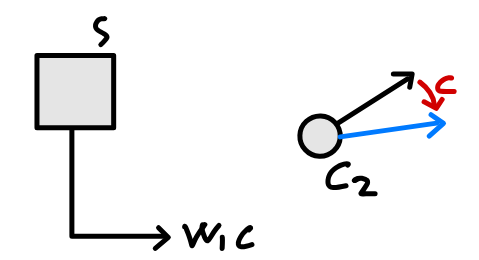
\includegraphics[width=\linewidth]{images/FL5.png}
    \label{fig:Scaled Dot Product Attention}
    \vspace{-10pt}
\end{wrapfigure}
The goal of many federated learning methods is to make each client follow, as closely as
possible, the \textbf{ideal update direction}. This ideal direction corresponds to the
update that would be obtained if \textbf{all data were available in a single place} and the
model were trained using standard centralized optimization.

Such an ideal update is easy to compute in settings where:
\begin{compactitemize}
    \item all training data are stored on a single client; or
    \item clients send both their \textbf{model parameters and gradients} to a central
    server.
\end{compactitemize}

In these cases, the server could aggregate all gradients, compute the global update
direction, and send it back to the clients. Each client would then use this information to
\textbf{correct its local update}, thereby avoiding the drift caused by non-IID data.

The main challenge is that \textbf{directly exchanging gradients is communication
expensive}, especially in large-scale federated systems. This motivates the need for
methods that \textbf{efficiently approximate the global correction} while maintaining low
communication overhead.

\subsection{SCAFFOLD}

\begin{wrapfigure}{r}{0.4\textwidth}
    \centering
    \vspace{-10pt}
    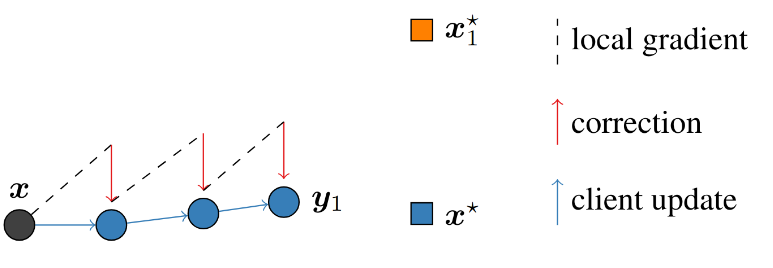
\includegraphics[width=\linewidth]{images/FL6.png}
    \label{fig:Scaled Dot Product Attention}
    \vspace{-10pt}
\end{wrapfigure}
\textbf{SCAFFOLD}  introduces a principled way to mitigate the
\textbf{client drift problem} by correcting the local update direction on each client.
The key idea is to adjust the local gradients so that they better align with the
\textbf{ideal global update direction}.

When client $i$ trains on the current global model $w$, instead of using the raw local
gradient $\nabla L_i(w)$, SCAFFOLD uses an \textbf{adjusted local gradient}:
\[
g_i(w) = \nabla L_i(w) - c_i + c,
\]
which pulls the client’s update direction closer to the global direction, thereby reducing
drift caused by non-i.i.d.\ data.

The variables $c$ and $c_i$ are known as \textbf{control variates} and play a central role
in the algorithm.

\subsubsection{Meaning of the Control Variates}

The control variates in SCAFFOLD serve as variance-reduction terms that correct systematic
biases in local updates.

\begin{compactitemize}
    \item \textbf{Server control variate $c$:}  
    An estimate of the \textbf{global update direction}, i.e., the direction the model would
    follow if all data were centralized and joint training were possible.

    \item \textbf{Client control variate $c_i$:}  
    A client-specific correction term that captures how client $i$’s local updates
    \textbf{systematically deviate from the global direction}. It represents the typical
    drift induced by the client’s local data distribution.
\end{compactitemize}

By subtracting $c_i$ and adding $c$, each client removes its own bias and injects a global
signal, making its update closer to the ideal centralized update.

\subsubsection{Adjusted Local Gradient}

With control variates in place, client $i$ performs local training using:
\[
g_i(w) = \nabla L_i(w) - c_i + c.
\]

This adjustment has a clear interpretation:
\begin{compactitemize}
    \item $-c_i$ removes the client’s own drift;
    \item $+c$ injects an approximation of the global update direction.
\end{compactitemize}

As a result, local updates become more consistent across clients, even under strong data
heterogeneity.

\subsubsection{How SCAFFOLD Works Across Rounds}

\textbf{First round.}  
No correction is applied. Each client trains normally on the initial global model $w$.

\textbf{End of the first round.}  
Each client computes its initial control variate $c_i$, typically as the average gradient
observed during local training on the server-provided model, and sends it to the server.

\textbf{Server update.}  
The server aggregates the received client control variates to form a global estimate:
\[
c = \frac{1}{N} \sum_{i=1}^{N} c_i,
\]
which approximates the global update direction.

\textbf{Subsequent rounds.}  
From the second round onward, each client uses the adjusted gradient
\[
g_i(w) = \nabla L_i(w) - c_i + c,
\]
thereby correcting its local updates using the global signal $c - c_i$.


\begin{figure}[H]
    \centering
    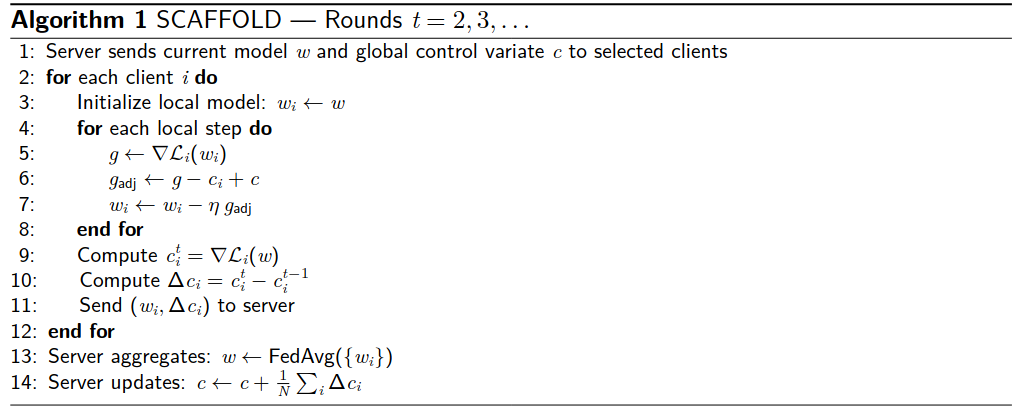
\includegraphics[width=1
    \textwidth]{images/FL7.png}
    \caption{Local Training in Rounds $t \ge 2$}
    \label{fig:MHA2}
\end{figure}

\subsubsection{Take-Home Message}

\textbf{Benefit}:  
SCAFFOLD significantly mitigates client drift by reducing the variance of local updates.
It provably converges faster than FedAvg under partial participation by better aligning
local optimization steps with the global objective.

\textbf{Strengths}:  
Client-side correction substantially improves upon FedAvg’s naive averaging, especially
in challenging non-i.i.d.\ scenarios, leading to faster and more stable convergence.

\textbf{Limitations}:  
Since SCAFFOLD acts only on the client side, it may not be sufficient in highly complex
settings or under extreme heterogeneity. In such cases, additional \textbf{server-side
strategies} may be required to further improve performance.

\section{Prototype-based Approach}

\subsection{Motivation for Prototype Sharing}

Model or gradient averaging methods (e.g., FedAvg-style aggregation) may become suboptimal
when client data distributions are highly heterogeneous. This is particularly evident in
settings where each client observes \textbf{different subsets of classes} or highly
imbalanced class distributions.

In such scenarios, directly averaging model parameters or gradients can lead to
inconsistent updates, since local models may specialize on different classes and develop
very different internal representations. As a result, aggregation at the parameter level
may fail to capture a coherent global structure.

An alternative idea is to share a more \textbf{interpretable intermediate
representation}. Instead of exchanging full models or gradients, clients can communicate
\textbf{class prototypes}, i.e., class-wise feature representations that summarize the
essential characteristics of each class observed locally.

\begin{infobox}[What are class prototypes?]
    A \textbf{class prototype} is a representative feature vector associated with a specific
    class. It is typically computed as the average of the feature embeddings of all samples
    belonging to that class:
    \[
    \mathbf{p}_c
    =
    \frac{1}{|\mathcal{D}_c|}
    \sum_{(x,y)\in\mathcal{D}_c,\; y=c}
    \phi(x),
    \]
    where $\phi(x)$ denotes the feature representation produced by the model and
    $\mathcal{D}_c$ is the set of samples of class $c$.
    
    Class prototypes:
    \begin{compactitemize}
        \item capture the \textbf{semantic essence} of a class in feature space;
        \item are \textbf{compact and interpretable} compared to full model parameters;
        \item can be shared across clients to \textbf{align feature representations} without
        exchanging raw data.
    \end{compactitemize}
\end{infobox}

The underlying hypothesis is that, by sharing and aligning these prototypes, clients can
build a \textbf{consistent global understanding of each class}. This promotes better
generalization across clients and mitigates the negative effects of data heterogeneity,
especially in class-incremental or label-skewed settings.

\subsection{FedProto}

\subsubsection{FedProto Algorithm}

\textbf{FedProto}  is a prototype-based federated learning algorithm designed
to address strong data heterogeneity, especially in scenarios where clients observe
different or non-overlapping sets of classes.

At each communication round, each client $i$ computes a set of \textbf{class prototypes}
$p_{i,c}$, one for each class $c$ present in its local dataset. Given a feature extractor
$f_i$, a classifier $g_i$, and a local dataset $D_i$, the prototype for class $c$ is computed
as:
\[
p_{i,c}
=
\mathbb{E}_{(x,y)\sim D_i}
\bigl[ f_i(x) \;:\; y = c \bigr].
\]

Instead of sending full model parameters or gradients, clients send only their local class
prototypes to the server. The server then aggregates the received prototypes by averaging
them class-wise to obtain a set of \textbf{global prototypes} $\bar{p}_c$ for each class $c$.

\subsubsection{Prototype-Based Regularization}

After aggregation, the server sends the global prototypes back to the clients. Each client
then augments its local training objective with a prototype regularization term:
\[
\mathcal{L}^{\text{FedProto}}_i
=
\mathcal{L}^{\text{local}}_i
+
\lambda
\sum_c
\left\|
p_{i,c} - \bar{p}_c
\right\|_2^2,
\]
which penalizes the discrepancy between the local prototype $p_{i,c}$ and the
corresponding global prototype $\bar{p}_c$.

This regularization encourages the feature representations learned by different clients to
remain \textbf{aligned in feature space}, effectively mitigating the impact of heterogeneous
label distributions.

\subsubsection{Inference}

At inference time, classification can be performed using a \textbf{nearest-mean
classifier}. Given an input sample $x$, the predicted label is:
\[
\hat{y}
=
\arg\min_c
\left\|
f(x) - \bar{p}_c
\right\|_2.
\]

This inference strategy naturally leverages the global prototypes as class representatives
and is particularly effective when class distributions differ across clients.

\subsubsection{Benefits and Empirical Results}

\textbf{Efficiency.}  
Prototype vectors are signiicantly smaller than full model updates, resulting in reduced
communication costs since only prototypes are exchanged instead of entire model
parameters.

\textbf{Effectiveness.}  
By regularizing local representations toward global prototypes, FedProto consistently
outperforms FedAvg and similar aggregation-based methods on heterogeneous benchmarks,
achieving higher accuracy and more stable convergence.

Empirical results show improved handling of scenarios with non-overlapping class
distributions across clients, demonstrating that FedProto enables effective knowledge
sharing beyond raw parameter averaging.

\subsubsection{FedProto Use-Cases}

FedProto is flexible and can be applied in multiple federated learning settings:

\begin{compactitemize}
    \item \textbf{Standard FL:}  
    FedProto can be combined with parameter aggregation methods (e.g., FedAvg) to learn
    a single global model while benefiting from prototype-based alignment.

    \item \textbf{Personalized FL:}  
    Clients can fine-tune their models on local data while sharing knowledge through class
    prototypes, enabling personalization without sacrificing global consistency.

    \item \textbf{Model-Heterogeneous FL:}  
    Since FedProto operates in feature space rather than parameter space, it naturally
    supports scenarios where clients have different model architectures, which makes
    standard parameter-wise aggregation infeasible.
\end{compactitemize}

\end{document}